%---------------------------------------------------
% University of Sussex thesis template
% Last Edit by Fabrizio Miano, Oct 2017
%---------------------------------------------------
%!TeX root = ../main.tex
\documentclass[a4paper,11pt,oneside,spanish]{memoir}
\usepackage[spanish, es-tabla, es-notilde, es-lcroman, es-nodecimaldot]{babel}


\input{metadata_spanish}
\RequirePackage{latex/atlaslatexpath}
\usepackage{latex/packages}
\usepackage{latex/atlasxref_spanish}
\usepackage{definitions}


\graphicspath{{./figures/}} % directory with all the pictures


%---------------------------------------------------
% BEGIN DOCUMENT
%---------------------------------------------------
\begin{document}
% --- to fix figure numbers
\makeatletter
\renewcommand{\counterwithin}{\@ifstar{\@csinstar}{\@csin}}
\makeatother



%---------------------------------------------------
% PREAMBLE: roman page numbering i, ii, iii, ...
%---------------------------------------------------
\pagestyle{custom}% Set page style to custom
\chapterstyle{hansen} % Set chapter style

{
    \frontmatter
    \pagenumbering{roman}
    \clearpage%%%%%%%%%%%%%%%%%%%%%%%%%%%%
%% TITLE PAGE: The title page should give the following information:
%%	(i) the full title of the thesis and the sub-title if any;
%%	(ii) the full name of the author;
%%	(iii) the qualification aimed for;
%%	(iv) the name of the University of Sussex;
%%	(v) the month and year of submission.
\pagestyle{empty}
% \begin{titlepage}
	\begin{center}

		\includegraphics[width=4cm]{UNLP_Logo.png}\\[1.5cm]% \bigskip

		{\LARGE \textsc{\myUni}}\\[0.3cm]
		{\Large \textsc{\myFaculty}}\\[0.3cm]
		{\Large \textsc{\myDepartment}}\\[2cm]

		%\vspace*{.05\textheight}
		\hrule
		{\Large Trabajo de Tesis Doctoral}\\[1cm]
		
		{\Huge \textbf{\myTitle}}\\[1cm] % Thesis title
		{\Huge \textit{\mySubtitle}}\\[0.6cm]
		\hrule

		\vspace{1cm}

		{
			\Large
			Autor:\\
			% \href{https://www.linkedin.com/in/daniela-koeck-b27041993/}{\myName}
			\myName
		}\\[1.5cm]

		{
			\Large
			Directores:\\
			\mySupervisor
		}

		\vfill
		\large \today

	\end{center}
% \end{titlepage}

    \clearpage\newpage \vspace*{8cm}
\pdfbookmark[0]{Dedicación}{Dedicación} % Bookmark name visible in a PDF viewer
\thispagestyle{empty}

\begin{flushright}
   % \emph{En memoria de Ayla, que todos los dias me ilumina.}\\
   % \emph{A mis papás y hermano, por su infinito amor.}
\end{flushright}
 % Dedication page
    \clearpage\pagestyle{empty}% Set page style to empty
\pdfbookmark[0]{Agradecimientos}{Agradecimientos} % Bookmark name visible in a PDF viewer
\begin{center}
	\Huge \textsc{\textbf{Agradecimientos}}
	\hrulefill
\end{center}


% Antes que nada pido disculpas a quién no mencioné. Son muchas personas que se me cruzaron estos últimos años. De antemano les agradezco infinitamente a cada uno y todos ustedes.

En primer lugar quiero agradecer a Tere y Fran por la oportunidad que me brindaron de trabajar con ellos, en esta Universidad, y poder cumplir también mi sueño de trabajar en el CERN. Por todo el acompañamiento permanente, por la confianza que tuvieron en mí, por exigirme también cosas que yo no sabía que podía hacer. Sin ese acompañamiento y ayuda esta tesis no hubiera sido posible. 
Gracias Tere también por leer y corregir incontable cantidad de veces esta tesis, no hay Director/a que se dedique tanto a sus estudiantes de Doctorado como vos.

Al grupo de HEP La Plata. Por los almuerzos, las cervezas mensuales, las picadas. Especialmente quiero agradecer a mis compañeros de oficina y amigos Jean y Tomás. Compartir el día a día de este camino con ustedes hizo que todo sea aún más divertido. Por las jodas, risas, cafés, charlas y el estrés que también compartimos. También quiero agradecer Tomás y Fede del grupo de Buenos Aires con quienes compartí oficina, hikes y fiestas.

To all the conveners I had during these 5 years. To the people at EGamma, for their invaluable help and insight on physics. To Jan-Lukas, Nadezda, Ludovica, Ruggero, thanks for all the help I got these years. To the Exotics group, thank you very much Dan, Tamara, Marco, Bing. I can't thank you enough for following my work all these years and helping me every time I asked you. For the long discussions, the round-tables, the presentations, the questions, and your patience with me while I was learning. Thank you very much.

It is impossible to forget thanking all the amazing people I met at CERN. You all made my stays there the most beautiful experiences. To all the people from the UK I met. To Adam, for the countless jokes, the beers at CERN, or everywhere else. To Dani, Marco, Ondrej, for the enormous amount of beers, for the barbecues, dinners, and the friendship that remains every time I go there. To the Tower of the Bear (beer), composed alongside Dani and Fer, for the difficult hike to the Jira, and the not so slippery and snowy hike to Schilthorn. For all the laughs and good times. To Marcelo, not the Marcelo Vieira (football player), but the one who still gets confused for him anyway, haha. Thank you for your friendship all these years since the first afternoon we met at the Saint-Genis Hostel. For all the nightclub nights with the GIA, the dodgy parties you know existed but didn't in the end. The talks, the beers.

Gracias también a Jona y Aimé, que me recibieron con brazos abiertos para cenas, cervezas, juegos y charlas allá en Geneva.

A todos los deadlines, los reales y los que me ponía yo sólo. A las infinitas slides que preparé. A los scripts que me hacen la vida más fácil. A StackOverflow, y más al final a ChatGPT. A las Twikis, que aunque son muy difíciles de encontrar, tienen la información que necesitaba.

A la música, que siempre me acompaña. A los paisajes que vi en Suiza. A los lugares que conocí en Europa.

A mis amigos acá en Argentina. Por las cervezas, los memes, las charlas, por las noches de viceo al conter y al fifa, por las risas.

En mis últimos 15 años también tuve la suerte de compartir la vida con Ayla y Gina, mis dos perritas. También le agradezco a ellas, especialmente a Ayla, que aunque ya no esté siempre me acompaña, en silencio atrás mío, siguiendo cada paso, entendiendo todo. Esta tesis es dedicada a ella, porque me acompaño cuando más yo lo necesitaba, desde mis 12 años hasta mis 27, iluminando siempre mi vida con sus ojos color avellana. A Gina, que con su mirada sincera y fiel está siempre al lado mio.

Pa, Ma, Manu: este trabajo es también dedicado a ustedes, porque ante cualquier cosa de la vida sé que siempre puedo contar con su amor infinito. Gracias por enseñarme a hacerme preguntas, analizar todo y a tener pensamiento crítico. Gracias por las charlas en la mesa en donde siempre aprendo, aunque me hago el que no y que me las sé todas. Gracias por los hermosos días de invierno en la pandemia, haciendo “nesting”. Gracias por ser mis “housemates” durante un poco más de un año… y fueron los mejores! Gracias Pa por ser el mejor compañero de oficina que tuve aunque hablás a los gritos y no sabés conectar los auriculares todavía, jaja. Gracias Ma por estar siempre pendiente de lo que yo necesito, por las infinitas pizzas que comimos y tus datos random en las cenas. Gracias Manu por tu mirada y perspectiva distinta en las cosas de la vida. Aunque no lo creas, aprendo mucho de vos -- igual yo sigo siendo el favorito de Mamá. Gracias a los tres por esas tardes imaginando viajes mirando mapas, hablando un poco sin saber de algunos lugares, pero imaginándonos a los 4 juntos paseando por ahí. Gracias por su paciencia conmigo, por su ayuda, por su amor. Esta tesis es de ustedes como es mía.

Justo antes de venir a La Plata tuve la suerte de conocer a la persona más especial y más buena que conozco. Gracias Abril por estar al lado mío y acompañarme en estos últimos años. Como siempre te lo digo, sos lo mejor que me pasó. Gracias por escucharme, aconsejarme y ayudarme, todo en el camino a ser una mejor persona. Gracias por escuchar cada detalle del análisis y de tratar de entender lo que hago, aunque a veces ni yo puedo. Gracias por venir a visitarme a La Plata, gracias por nuestros viajecitos juntos. Gracias por todo tu amor.

Y a todos de los que me olvido, gracias!



\medskip

{
	\begin{flushright}
		Francisco Sili
	\end{flushright}
} % Acknowledgements page
    % \clearpage\input{FrontBackMatter_spanish/Declaration} % Declaration
    \clearpage% % Abstract

\thispagestyle{empty}
\pdfbookmark[0]{Resumen}{Resumen} % Bookmark name visible in a PDF viewer

% \begin{center}
%     %	\bigskip
%     {\normalsize \myUni \\} % University name in capitals
%     {\normalsize \myFaculty \\} % Faculty name
%     {\normalsize \myDepartment \\} % Department name
%     \bigskip\vspace*{.02\textheight}
%     {\Large \textsc{Tesis de Doctorado}}\par
%     \bigskip

%     {\rule{\linewidth}{1pt}\\%[0.4cm]
%     \Large \myTitle \par \mySubtitle} % Thesis title
%     \rule{\linewidth}{1pt}\\[0.4cm]

%     \bigskip
% 	{\normalsize por \myName \par} % Author name
%     \bigskip\vspace*{.06\textheight}
% \end{center}


{\centering\Huge\textsc{\textbf{Resumen}} \par}
\bigskip



Esta tesis presenta una búsqueda de nueva física en eventos que contienen un fotón y un jet de alto momento transverso, realizada con datos recolectados por el experimento \acs{ATLAS} a partir de colisiones protón-protón del \ac{LHC}, a energía de centro de masa de \(\sqs=13~\tev\).
La búsqueda consiste en la identificación de resonancias en la masa invariante del fotón y el jet - provenientes de partículas o de estados de alta masa no incluídos en el \ac{SM} - que se manifiestan como un exceso localizado de eventos sobre el fondo del \ac{SM}.
% Dado que no se observó un exceso estadísticamente significativo, se establecieron límites a \(95\%\) \acs{CL} en la sección eficaz de producción de resonancias Gaussianas genéricas.
Los resultados obtenidos permitieron establecer los límites más estrictos en la sección eficaz de producción de resonancias gaussianas genéricas y de aquellas predichas en dos modelos de física más allá del \ac{SM}.
Por un lado, un modelo de Quarks Excitados con diferentes acoplamientos (\(f\)) y diferentes sabores, \qstar (\(u^*/d^*\)), \cstar y \bstar, en el que para el caso de \(f=1\) se excluyeron masas de hasta \(6174\), \(3414\) y \(2493~\gev\), respectivamente.
Los límites en el modelo de \cstar corresponden a los primeros resultados obtenidos en experimentos del \acs{LHC}.
Por otro lado, se estudiaron modelos de Micro-Agujeros Negros, como los propuestos por Randall-Sundrum (Arkani-Hamed-Dimopoulos-Dvali) que consideran la existencia de una (seis) dimension(es) extra(s). En este caso, los resultados obtenidos permitieron excluir masas de hasta \(5347~\gev\) (\(7590~\gev\)).
A su vez, se realizó un estudio sobre las correcciones a las variables que describen el pasaje de los fotones por los calorímetros electromagnético y hadrónico, las cuales son imprescindibles para la correcta identificación de fotones en el detector \acs{ATLAS} y que resultó en una mejora sustancial al método tradicional. Se presentó, asimismo, un nuevo enfoque en el que las correcciones se realizan en el nivel más bajo de la reconstrucción de señales en el detector, siendo este de gran interés para la colaboración en vistas al futuro High-Luminosity \ac{LHC} y la utilización de algoritmos de Machine Learning.


\noindent 
 % Abstract page
}



%---------------------------------------------------
% TABLE OF CONTENTS, LISTS OF TABLES & FIGURES
%---------------------------------------------------
{
    \newpage
    \input{FrontBackMatter_spanish/Contents.tex}
}




%---------------------------------------------------
% MAIN THESIS TEXT: arabic page numbering 1, 2, 3, ...
% THESIS CONTENT - CHAPTERS
%---------------------------------------------------
\mainmatter
\pagenumbering{arabic}






% Possible quotes for chapters



% “Not only is the Universe stranger than we think, it is stranger than we can think.” Werner Heisenberg

% "Any sufficiently advanced technology is indistinguishable from magic." Arthur C. Clarke
% “Experiment is the sole judge of scientific truth.” Richard Feynman

% “There is a single light of science, and to brighten it anywhere is to brighten it everywhere.” Isaac Asimov
% “Nothing in life is to be feared, it is only to be understood. Now is the time to understand more, so that we may fear less.” Marie curie

% “There is a crack in everything. That's how the light gets in.” Leonard Cohen
% “If you wish to make an apple pie from scratch, you must first invent the universe.” Carl Sagan
% “I don't want to believe. I want to know.” Carl Sagan
% “If I have seen further it is by standing on the shoulders of Giants.” Isaac Newton
% "Only those who will risk going too far can possibly find out how far one can go." T. S. Elliot
% “Somewhere, something incredible is waiting to be known.” Carl Sagan



\acresetall
\chapter*{Introducción}
\addcontentsline{toc}{chapter}{Introducción}
\markboth{}{Introducción}

Nuestra mejor comprensión actual de la física de partículas viene dada por la \ac{SM}, una teoría que explica con éxito una amplia gama de resultados experimentales y predijo con precisión muchos fenómenos físicos diferentes. También, predijo la existencia de nuevas partículas, como el bosón de Higgs descubierto en 2012 por las colaboraciones \acs{ATLAS} y \acs{CMS}, que llevó a la concesión del Premio Nobel a François Englert y Peter Higgs al año siguiente. A pesar de su notable éxito, se sabe que el \ac{SM} es incompleto ya que no puede explicar una serie de observaciones experimentales, como la abrumadora evidencia astrofísica y cosmológica de la materia oscura, el problema de jerarquías, por qué solo hay tres familias de fermiones, entre otros. En las últimas décadas, surgieron muchas teorías para la nueva física \ac{BSM}, como \ac{SUSY}, que proporcionaron marcos teóricos bien motivados y prometedores para ampliar nuestra comprensión fundamental de la física de partículas y mejorar las deficiencias del \ac{SM}. Sin embargo, ninguna de las numerosas búsquedas de nueva física que se han llevado a cabo en los colisionadores de partículas en los últimos años ha podido aportar pruebas directas de la existencia de nuevas partículas o fuerzas, tal y como predecían estas teorías.

Una gran variedad de estos nuevos modelos teóricos predicen la existencia de partículas a altas energías. Para explorar estas regiones, especialmente la escala \tev, en el laboratorio \acused{CERN}\ac{CERN} se construyó el \ac{LHC}~\cite{LHC-Machine}. Instalado en un túnel circular de 27 kilómetros, es el mayor y más potente colisionador de partículas del mundo. Esta máquina es capaz de colisionar haces energéticos de protones a velocidades superiores a millones por segundo. La precisión y la elevada energía de los haces del \ac{LHC} permiten explorar energías en la escala del \tev, un rango energético nunca antes alcanzado en un colisionador de partículas. El \ac{LHC} colisiona protones en cuatro puntos de interacción, donde se encuentran los 4 experimentos principales del \ac{LHC}: \acused{ATLAS}\ac{ATLAS}, \acused{CMS}\ac{CMS}, \acused{LHCb}\ac{LHCb} y \acused{ALICE}\ac{ALICE}.
Entre los años 2015 y 2018 tuvo lugar un periodo de toma de datos denominado Run-2, en el que se colisionaron protones a \(\sqs=13~\tev\), y recogiendo un total de luminosidad integrada de \(140.01~\ifb\). En 2022 comenzó el \ac{LHC} Run-3, en el que se aumentó la energía del centro de la masa a \(\sqs=13.6~\tev\), y a finales de 2024 \ac{ATLAS} llego a recolectar \(183~\ifb\) de datos.

Uno de los experimentos más importantes del \ac{LHC} es el \ac{ATLAS} (\acl{ATLAS}), un detector multipropósito diseñado para realizar tanto medidas de precisión dentro del \ac{SM} como búsquedas de nuevos fenómenos asociados a la física \ac{BSM}. El detector \ac{ATLAS} está compuesto por distintos subdetectores que desempeñan diferentes papeles en la reconstrucción de las partículas en colisión. El \acl{ID} se encarga de medir las trazas de partículas cargadas, los calorímetros miden las deposiciones energéticas de fotones, electrones y diferentes hadrones, y finalmente el \acl{MS} permite medir las trayectorias de los muones. Entre ellos se encuentra un potente sistema magnético, que curva la trayectoria de las partículas cargadas. Por último, el detector \ac{ATLAS} dispone de un preciso sistema trigger que filtra los eventos de poco interés, reduciendo así la frecuencia del flujo de datos.
En cualquier experimento de física de altas energías, es habitual trabajar con simulaciones, tanto para los procesos conocidos del \ac{SM}, como para comprender las formas de las nuevas señales predichas por los escenarios \ac{BSM}. Esto añade otro grado de complejidad al experimento, ya que se requiere que las simulaciones describan de forma excelente los procesos físicos reales que se obtendrían de los datos reales.

La producción de fotones prompt a partir de colisiones \pp en el \ac{LHC} constituye una parte clave del programa de física \ac{ATLAS}, ya sea para medidas precisas de observables \ac{QCD}, o porque varios escenarios \ac{BSM} implican tener fotones prompt aislados en el estado final. Sin embargo, el principal proceso que tiene lugar en las colisiones \pp es la producción de jets, y a veces uno de estos jets tiene caracter'isticas muy similares a las que tendría un fotón, por lo que este jet se identifica erróneamente como un fotón. El proceso de identificación en \ac{ATLAS} constituye uno de los ingredientes principales en cualquier análisis de física. En el caso de los fotones, esta identificación se lleva a cabo estudiando la lluvia \ac{EM} iniciada por las partículas en el calorímetro utilizando diversas variables que describen la forma de éstas, y como se anticipó, se lleva a cabo utilizando los datos y las simulaciones. Sin embargo, se observó que la simulación no predecía correctamente los datos, lo que conducía a resultados incongruentes.
Una de las principales tareas de esta tesis es la corrección de las variables utilizadas para la identificación de fotones. El método actual para corregir las variables se denomina \ac{FF}, que se mejoró drásticamente en este trabajo. Además, se estudió otro enfoque, en el que se pueden realizar modificaciones en variables de nivel inferior para as'i corregir simultáneamente todas las variables utilizadas para identificar fotones.

En el párrafo anterior se mencionó que los fotones prompt son de gran importancia para las búsquedas \ac{BSM}. En particular, en el estado final fotón+jet, la masa invariante sigue una forma descendente muy suave, proporcionando un escenario excelente para las búsquedas de bump, donde se pueden buscar diferentes partículas que decaen a un par fotón+jet. Dos de los modelos teóricos que pretenden dar respuesta a las diferentes carencias del \ac{SM} predicen la existencia de este tipo de partículas. El primero da una explicación de por qué existen tres familias de fermiones, y propone que los quarks no son partículas fundamentales sino estados ligados de otras más fundamentales que experimentan una fuerza desconocida. Entonces, deberían observarse estados de \ac{EQ} (\qstar) en colisiones \pp en el \ac{LHC} dependiendo de si el valor de la escala de composición \(\Lambda\) es menor que la energía del centro de masa. Estos \ac{EQ} decaerían en un par de fotón y jet, dejando una \textit{bump} en la distribución de \myj alrededor de la masa del \ac{EQ}. El segundo modelo, con la introducción de dimensiones extra, intenta proponer una solución para el problema de jerarquías. Ciertos tipos de modelos de dimensiones extra predicen que la escala fundamental de Planck \(m_P\) en las \(4 + n\) dimensiones (siendo \(n\) el número de dimensiones espaciales extra) está en la escala \tev, y por tanto accesible en colisiones \pp en la \(\sqs=13~\tev\).
En tal escala \TeV, a partir de una masa umbral \(m_{\text{th}}\), se podr'ian producir \ac{QBH} en colisiones \pp del \ac{LHC} y luego decaer en un pequeño número de partículas de estado final incluyendo pares fotón-quark/gluón antes de que sean capaces de termalizarse. En este caso podría observarse una amplia estructura resonante justo por encima de \(m_{\text{th}}\) sobre la distribución de \myj del \ac{SM}. Bajo esta teoría se estudian dos modelos particulares, que proponen diferentes números de dimensiones extra: el modelo RS1 de Randall-Sundrum propone un total de 5 dimensiones espacio-temporales, y el modelo ADD de Arkani-Hamed, Dimopoulos y Dvali, que cuenta con un total de 10 dimensiones espacio-temporales.
Por último, dada la suavidad de la distribución \myj, es posible realizar una búsqueda agnóstica del modelo sobre este fondo, en la que se considera que la señal sigue una resonancia de forma gaussiana. Este tipo de búsqueda proporciona una interpretación más general del estudio, ya que permite comparar con cualquier modelo de teoría que proponga una resonancia de forma Gaussiana.


Estudios previos similares de b\'usquedas de resonancias en el estado final de \gammajet considerando los mismos modelos teóricos han sido llevados a cabo. estableciendo as'i límites superiores a las teorías. El último resultado de \ac{ATLAS} utilizó \(36.7~\ifb\) y excluyó los modelos de \qstar con masas de hasta \(5.3~\tev\), los \ac{QBH} del tipo RS1 hasta \(4.4~\tev\) y los \ac{QBH} del tipo ADD hasta \(7.1~\tev\). Por otro lado, \ac{CMS} también realizó estudios similares utilizando \(138~\ifb\), donde estudiaron modelos de \ac{EQ} que separaron en resonancias livianas (\qstar) y pesadas (\bstar), estableciendo límites m\'as estrictos de \(6.0~\tev\) y \(2.2~\tev\), respectivamente. \ac{CMS} también estudió los modelos de \ac{QBH} ADD y RS1, en los que los límites superiores de las masas se extienden hasta \(7.5~\tev\) y \(5.2~\tev\), respectivamente.

El trabajo principal de esta tesis es la búsqueda de resonancias de alta masa en el estado final fotón+jet. La búsqueda se realiza utilizando el conjunto completo de datos Run-2 recolectados a una energía de centro de masa de \(\sqs=13~\tev\), utilizando un total de \(140.01~\ifb\). Se estudian los modelos \ac{EQ} y \ac{QBH}, así como la búsqueda de señales genéricas de forma gaussiana.
En particular, para los modelos de \acp{EQ}, se separan las señales en \qstar (\(u^*/d^*\)), \cstar y \bstar, siendo este trabajo el primero en el \ac{LHC} considerando el sabor charm, gracias a un novedoso algoritmo de tagging de sabores, que proporciona un excelente rendimiento.




La tesis se divide en cuatro partes.
La \Part{\ref{part:theory}} describe el marco teórico y las motivaciones del trabajo, donde se describe brevemente el \ac{SM} y se discuten los dos modelos teóricos que motivan la b\'usqueda de f'isica \ac{BSM} de este trabajo.

La \Part{\ref{part:exp_setup}} contiene dos capítulos en los que el primero (\Ch{\ref{ch:atlas}}) describe detalladamente el \ac{LHC} y el detector \ac{ATLAS}, haciendo hincapié en las distintas partes del detector. En el \Ch{\ref{ch:objects}}, se analizan los métodos utilizados para la reconstrucción e identificación de los distintos objetos f'isicos.

En la \Part{\ref{part:pid}} se explican los diferentes algoritmos utilizados para la identificación de fotones. Primero, en el \Ch{\ref{ch:pid_ss}}, se discuten las variables utilizadas para la identificación de fotones, cómo se optimiza y cómo se realizan las medidas de eficiencia de la identificación. Luego, en el \Ch{\ref{ch:ss_corrections}}, se presentan los métodos diferentes, obtenidos en esta tesis, para corregor las variables simuladas que se usan para realizar la identificación de fotones.

Finalmente, la \Part{\ref{part:search}} presenta la búsqueda de resonancias de \gammajet en el rango de altas masas. El \Ch{\ref{ch:strategy}} comienza discutiendo la estrategia general de análisis y establece los métodos estadísticos que se utilizarán. A continuación, en el \Ch{\ref{ch:samples}}, se describen las muestras que se utilizan tanto para los modelos teóricos como para los fondos del \ac{SM}. La selección de eventos y las definiciones de las regiones de señal que se utilizan en la búsqueda se presentan en el \Ch{\ref{ch:evt_selection}}. El modelado de la señal y las incertezas sistemáticas teóricas y experimentales se describen en el \Ch{\ref{ch:signals}}, que constituyen uno de los puntos más importantes y desafiantes de cualquier búsqueda. Adem\'as, es crucial tener un excelente conocimiento de los fondos del \ac{SM}. Para ello, en el \Ch{\ref{ch:bkg}}, se estudian los dos fondos principales, donde se utiliza un modelo funcional para modelar el fondo total del \ac{SM}. Por último, en el \Ch{\ref{ch:results}} se presentan y discuten los resultados obtenidos en esta búsqueda.
\acresetall


\part{Motivación Teórica}
\label{part:theory}
\chapter{Motivación teórica}
\label{ch:theory}
% \epigraph{\emph{\enquote{Nothing in life is to be feared. It is only to be understood. Now is the time to understand more, so that we may fear less}}}{Marie Curie}


Esta tesis se centra en la búsqueda de nuevas partículas predichas por diferentes escenarios más allá del \ac{SM}. En este capítulo se presenta un resumen de los principales conceptos del \ac{SM} utilizados a lo largo de esta tesis. Además, se describen las interacciones hadrónicas en una colisión \pp y en el proceso de producción de fotones \textit{prompt}.
A continuación, en \Sect{\ref{sec:theory:bsm}} se ofrece una vista general de las limitaciones actuales del \ac{SM} y cómo, con modelos de física \ac{BSM}, se pretenden resolver estos problemas.
Por último, en la \Sect{\ref{sec:theory:mc_simulation}}, el capítulo termina con cómo se simulan estos procesos del \ac{SM} utilizando \ac{MC}, mostrando los diferentes pasos y herramientas para hacerlo.




\section{El Modelo Estándar}
\label{sec:theory:sm}

El \acf{SM} de física de partículas es la teoría matemática que describe todas las partículas elementales conocidas y sus interacciones.
La teoría se ha ido desarrollando a lo largo de varias decadas y tras numerosos experimentos que respaldaron sus predicciones, se ha convertido en la teoría más completa de la física de partículas.

El \ac{SM} logra describir tres de las cuatro fuerzas fundamentales de la naturaleza: las interacciones \ac{EM}, débil y fuerte, las cuales actúan en distintos rangos.
La gravedad, la cuarta fuerza de la naturaleza, aunque no está incluida en el \ac{SM}, es la más débil de las interacciones y tiene un alcance infinito.
Las tres fuerzas fundamentales del \ac{SM} resultan del intercambio de partículas que pertenecer al grupo de \textit{bosones}. Las partículas de materia, los \textit{fermiones}, interactúan entre ellas transfiriendo cantidades discretas de energía a través del intercambio de estos bosones.



\subsection{Partículas elementales y sus interacciones}
\label{subsec:theory:sm:particles_interaction}

Según el \ac{SM}, toda la materia está formada por fermiones, que son partículas que siguen la estadística de Fermi-Dirac y tienen spin semi-entero. Estos fermiones interactúan entre sí mediante el intercambio de bosones, que son partículas de spin entero, siguiendo la estadística de Bose-Einstein. Hasta la fecha no ha habido ningún experimento capaz de encontrar pruebas de que estas partículas tengan estructura interna.

\begin{figure}[ht!]
    \centering
    \includegraphics[width=\linewidth]{2_theory/sm}
    \caption{Partículas del \ac{SM} y sus propiedades. Todos los fermiones participan en la interacción débil, pero sólo los quarks interaccionan con los gluones, mientras que tanto los quarks como los leptones cargados interaccionan mediante la fuerza \ac{EM}. Los neutrinos, al ser neutros e incoloros, sólo interaccionan con los bosones \Wboson y \Zboson a través de la fuerza débil. Por último, el gravitón, aunque aún no se ha descubierto, debería ser el correspondiente portador de la fuerza gravitatoria. Extraído de la \Refn{\cite{SM_diagram}}.}
    \label{fig:theory:sm:particles_interaction:particles}
\end{figure}

Los fermiones se dividen en dos tipos de partículas elementales: los leptones y los quarks. Existen seis leptones clasificados según su carga que se dividen en tres familias o generaciones, ordenadas en función de su masa. Las partículas de las generaciones superiores tienen mayor masa y son muy inestables, decayendo en leptones de generaciones inferiores. Por esta razón, la materia se construye a partir de leptones de primera generación. Los leptones son: electrón (\(e\)), muón (\(\mu\)) y tau (\(\tau\)), con sus respectivos neutrinos: neutrino electrón (\(\nu_{e}\)), neutrino muón (\(\nu_{\mu}\)) y neutrino tau (\(\nu_{\tau}\)).
También hay seis antileptones que tienen carga eléctrica opuesta a la de los leptones. El electrón, el muón y el tau tienen carga eléctrica y una masa considerable, mientras que los neutrinos son eléctricamente neutros y tienen una masa muy pequeña (aunque en el \ac{SM} es estrictamente cero).

Del mismo modo, hay seis sabores (flavours) de quarks, también con sus respectivas antipartículas: up (\(u\)), down (\(d\)), charm (\(c\)), strange (\(s\)), top (\(t\)) y bottom (\(b\)). Los quarks también presentan otra propiedad que es el número cuántico de color y sólo se mezclan de tal manera que forman objetos sin color. En la \Fig{\ref{fig:theory:sm:particles_interaction:particles}} se muestra un resumen de los quarks y sus propiedades.


Cada una de las tres fuerzas en el \ac{SM} se describe mediante una \ac{QFT}.
La fuerza fuerte, mediada por gluones sin masa, es responsable de la interacción entre los quarks que aunque no tienen carga eléctrica poseen carga de color. A pesar de que estos no tienen masa, la interacción fuerte se hace más fuerte a bajas energías, confinando quarks y gluones dentro de hadrones debido a la propiedad de libertad asintótica y a la propiedad de \textit{confinamiento}, las cuales serán discutidas más adelante.
La fuerza \ac{EM} entre partículas cargadas está mediada por fotones. Los fotones no tienen masa y, en consecuencia, la interacción tiene un alcance infinito.
Por último, la interacción débil está mediada por los bosones masivos \Wboson y \Zboson, que dan lugar a interacciones de corto alcance. Las propiedades fundamentales de estos bosones también se muestran en la \Fig{\ref{fig:theory:sm:particles_interaction:particles}}.









\subsection{Breve descripción matemática del Modelo Estándar}
\label{subsec:theory:sm:mathematical}

El \ac{SM} es una teoría de campos renormalizable basada en simetrías locales que proporciona una descripción de las partículas fundamentales y sus interacciones: la fuerte, la débil y la \ac{EM}. Estas interacciones aparecen por el requisito de que la teoría es invariante bajo transformaciones gauge locales del grupo de simetría:
\begin{equation*}
    SU(3)_{C} \times SU(2)_{L} \times U(1)_{Y},
\end{equation*}
donde \(Y\) es la hipercarga, \(L\) la helicidad izquierda y \(C\) la carga de color, y representan las cantidades conservadas del grupo de simetría. Cada transformación gauge local puede ser absorbida dentro de un campo de gauge, con las excitaciones de los campos gauge llamadas bosones gauge. El sector \ac{EW} del \ac{SM} \(SU(2)_{L} \times U(1)_{Y} \to U(1)_{\text{EM}}\) describe las interacciones débil y \ac{EM}, tras el mecanismo de ruptura espontánea de simetría en virtud del potencial de Higgs. El grupo no abeliano \(SU(3)_C\), con carga de color, describe las interacciones fuertes entre quarks y gluones y la teoría se conoce como \ac{QCD}~\cite{Ellis-1996-book}.

En principio, las partículas incluidas en el \ac{SM} carecen de masa a diferencia de las partículas observadas en la naturaleza. Aunque las ecuaciones de la interacción \ac{EW} describen correctamente partículas como el fotón, no dan cuenta de las masas de los bosones \Wboson y \Zboson. Para solucionar este problema se introdujo el concepto de \ac{EWSB}, conocido como mecanismo de Brout-Englert-Higgs~\cite{Higgs-1964_1,Higgs-1964_2,Higgs-1966,Englert_Brout-1964}. Este mecanismo explica cómo los bosones \Wboson y \Zboson adquieren masa a través de la ruptura espontánea de la simetría \ac{EW}, causada porque el campo escalar de Higgs adquiere un \ac{VEV} distinto de cero. Además, predice la existencia de una nueva partícula escalar, dando lugar a un nuevo bosón masivo de spin 0, denominado bosón de Higgs. Esta partícula fue confirmada experimentalmente en 2012 por las colaboraciones \ac{ATLAS}\acused{ATLAS} y \ac{CMS}\acused{CMS} en el \ac{LHC}\acused{LHC}, con una masa medida de \(125.11 \pm 0.11~\gev\)~\cite{ATLAS-HiggsObservation,CMS-HiggsObservation,ATLAS-Higgs-2024}.








\subsubsection{The interaccón \acl{EW}}

Las interacciones \ac{EW} satisfacen la simetría de gauge del grupo \(SU(2)_L \times U(1)_Y\). El grupo \(SU(2)_L\), llamado isospín débil actúa sólo sobre los fermiones de quiralidad izquierda y \(U(1)_Y\) es el grupo de hipercarga que actúa sobre ambas quiralidades de forma vectorial.
El grupo \(SU(2)_L \times U(1)_Y\) tiene cuatro generadores, de los cuales tres pertenecen al isospín débil: \(T_i = \frac{\sigma_i}{2}\), siendo \(i = 1,\, 2,\, 3\) y \(\sigma_i\) las matrices de Pauli y uno al grupo de hipercarga: \(\frac{Y}{2}\). Los fermiones izquierdos se transforman como dobletes bajo \(SU(2)_L\), \(f_L \ra e^{i T_i \theta_i} f_L\) con
\begin{equation}
    f_L = \mqty( \nu_L\\ e_L ), \mqty( u_L\\ d_L ), \dots,
\end{equation}
mientras que los fermiones derechos se transforman como singletes \(f_R \ra f_R\) con
\begin{equation}
    f_R = e_R, \, u_R,\, d_R, \dots.
\end{equation}
Esta distinción entre izquierdos y derechos implica que la teoría \(SU(2)_L \times U(1)_Y\) es una teoría quiral.
Por otro lado, la carga eléctrica está relacionada con la tercera componente del isospín débil \(T_3\) y la hipercarga \(Y\), según la fórmula de Gell-Mann Nishijima:
\begin{equation}
    Q = T_3 + \frac{Y}{2}
\end{equation}

El número de bosones de gauge asociados coincide con el número de generadores del grupo de simetría. Para el isospín débil hay 3 bosones \(SU(2)_L\): \(W_{\mu}^1,\, W_{\mu}^2,\, W_{\mu}^3\), y para \(U(1)\) se tiene un bosón de hipercarga: \(B_{\mu}\).
La simetría global \(SU(2)_L \times U(1)_Y\) se convierte en local, sustituyendo en la lagrangiana la derivada de los campos por la derivada covariante:
\begin{equation}
    \label{eq:theory:sm:mathematical:ew:covariant_derivative}
    D_{\mu} = \partial_{\mu} - ig \frac{\tau^i}{2} W_{\mu}^i - i g' \frac{Y}{2} B_{\mu},
\end{equation}
donde \(g\) es la constante de acoplamiento de \(SU(2)_L\) y \(g'\) de \(U(1)_Y\).

La densidad lagrangiana \ac{EW} puede escribirse entonces como la suma del lagrangiano fermiónico con las interacciones de gauge y los términos cinéticos para los campos de gauge introducidos:
\begin{equation}
    \mathcal{L}_{\text{EW}} = 
    - \frac{1}{4} F_{\mu\nu}^i F^{\mu\nu}_i
    - \frac{1}{4} B_{\mu\nu} B^{\mu\nu}
    + \sum_{f = \ell, q} \bar{f} i \gamma^{\mu} D_{\mu} f,
\end{equation}
donde los tensores de campo de Yang-Mills \(F_{\mu\nu}^i\) para \(SU(2)_L\) y \(B_{\mu\nu}^i\) para \(U(1)_Y\) se definen como:
\begin{gather}
    F_{\mu\nu}^i = \partial_{\mu} W_{\nu}^i  -  \partial_{\nu} W_{\mu}^i + g \epsilon_{ijk} W_{\mu}^jW_{\nu}^k \\
    B_{\mu\nu} = \partial_{\mu} W_{\nu}  -  \partial_{\nu} W_{\mu}.
\end{gather}




\subsubsection{El mecanismo de Higgs}

La formulación hasta ahora descripta no incluye en las masas de ninguna de las partículas. Esto se debe a que al agregar términos de masa explícitos al lagrangiano (como por ejemplo \(m \psi \hat{\psi}\) o \(m_B^2 B^{\mu}B_{\mu}\)), el mismo pierde la invarianza \ac{EW}. La forma de incluir masas a la teoría es mediante el mecanismo de Higgs. Para ello se asume la existencia de un campo de spin 0, denominado campo de Higgs. El mismo es un doblete en el espacio \(SU(2)\) y tiene hipercarga no nula en \(U(1)\), pero es un singlete en el espacio de color. Los bosones de gauge y los fermiones pueden interactuar con este campo, y en su presencia dejan de tener masa nula. Si bien el Lagrangiano conserva la simetría \(SU(2)\) y \(U(1)\), el estado fundamental no, en lo que se denomina un rompimiento espontáneo de simetría.

El sector de Higgs del Lagrangiano viene dado por:
\begin{equation}
    \mathcal{L}_{\text{Higgs}} = \left(D^{\mu} \phi\right)^{\dagger} \left(D_{\mu} \phi\right) - V(\phi)
\end{equation}
donde \(\phi\) es un campo escalar complejo en la representación \(SU(2)\):
\begin{equation}
    \Phi = \mqty( \phi_{+} \\ \phi_0 ) = \frac{1}{\sqrt{2}} \mqty(\phi_1 + i \phi_2 \\ \phi_3 + i \phi_4),
\end{equation}
con hipercarga \(U(1)\) \(Y=+1\), donde \(\phi_{+}\) y \(\phi_{0}\) son complejos con carga eléctrica \(+1\) y \(0\), respectivamente y la derivada covariante viene dada por la \Eqn{\ref{eq:theory:sm:mathematical:ew:covariant_derivative}}. La razón de tener la simetría adicional \(U(1)_Y\) es para que la teoría produzca un bosón de gauge sin masa asociado al fotón. Se requiere que el potencial de Higgs \(V(\phi)\) tenga la forma
\begin{equation}
    V(\phi) = -\mu^2 \phi^{\dagger} \phi + \lambda \left(\phi^{\dagger} \phi\right)^2
\end{equation}
para garantizar la renormalizabilidad de la teoría y la invariancia de \(SU(2)\) y \(U(1)\). El parámetro \(\lambda\) tiene que ser positivo para que el potencial tenga un mínimo, de forma que el comportamiento del campo venga determinado entonces por \(\mu\). Para \(\mu^2 > 0\), el campo genera un \ac{VEV} distinto de cero (\(v := \phi^{\dagger} \phi\)) que rompe espontáneamente la simetría. El potencial \(V(\phi)\) tiene la forma conocida de un sombrero mexicano con infinitos estados degenerados con energía mínima que satisface \(v = \sqrt{-\mu^2/\lambda}\). De estos infinitos estados, es habitual utilizar:
\begin{equation}
    \expval{\Phi} = \frac{1}{\sqrt{2}} \mqty(0\\v)
\end{equation}
con \(\phi_1 = \phi_2 = \phi_4 = 0\), \(\phi_3 = v\).

Para estudiar el espectro de partículas, se estudia el campo alrededor del mínimo utilizando una expansión en la dirección radial:
\begin{equation}
    \phi = \frac{1}{\sqrt{2}} \mqty(0 \\ v + H(x)),
\end{equation}
donde \(H(x)\) son excitaciones del estado fundamental alrededor del mínimo pero en la dirección radial del potencial.
Debido a la invariancia de gauge del potencial para excitaciones alrededor de los mínimos de la circunferencia y de acuerdo con el teorema de Goldstone, uno debería en principio tener tres bosones escalares sin masa asociados a los grados de libertad no radiales del campo. La arbitrariedad de gauge permite que los bosones de Goldstone sean absorbidos por los bosones \Wboson y \Zboson (proporcionan las polarizaciones longitudinales adquiridas por los campos gauge). El desarrollo en la dirección radial da la masa de la excitación \(H\), \(\sqrt{2\lambda}\nu\) que es la masa del bosón de Higgs, y los acoplamientos cúbicos y cuárticos de este bosón. De esta manera, las masass de los bosones del \ac{SM} tienen la forma:
\begin{align}
    m_{g} &= 0\\
    m_{\gamma} &= 0\\
    m_{\Wboson} & = \frac{g v}{2}\\
    m_{\Zboson} & = \frac{g}{2} \sqrt{g^2 + g'^2}\\
    m_{H} & = \sqrt{2\lambda}\nu
\end{align}

Los términos de acoplamiento tipo Yukawa al campo de Higgs dan masas a los fermiones del \ac{SM}:
\begin{equation}
    \mathcal{L}_{\text{Yuk}} = g_f \left(\bar{\psi}_L \phi \psi_R + \phi^{\dagger} \bar{\psi}_R \psi_L\right),
\end{equation}
siendo este una invariante \(SU(2)\). La constante de acoplamiento \(g_f\) describe el acoplamiento entre el doblete de Higgs y los fermiones. Haciendo una expansión del campo similar a la realizada anteriormente y sustituyendo en el Lagrangiano de Yukawa, se obtienen términos que indican las masas de los fermiones como
\begin{equation}
    m_f = \frac{g_f v}{\sqrt{2}}.
\end{equation}


\subsubsection{La interacción fuerte}
\label{subsubsec:theory:sm:mathematical:qcd}

El enorme esfuerzo por describir el gran espectro de resonancias de mesones y bariones que se descubrieron durante la década de 1950, llevó a Gell-Mann y Zweig a proponer en 1964 el modelo de los quarks~\cite{Gellmann-1964,Zweig-1964_1,Zweig-1964_2}, que afirma que los hadrones son en realidad compuestos de constituyentes más pequeños. Zweig denominó a las partículas elementales \textit{aces} mientras que Gell-Mann las llamó \textit{quarks}, pero finalmente la teoría pasó a llamarse modelo de los quarks.

El modelo de los quarks se formalizó en la teoría de \ac{QCD} con quarks que llevan un número cuántico adicional llamado carga de color, \(C=R,G,B\). Sin carga de color, los quarks dentro de algunos hadrones existirían en estados cuánticos simétricos, en violación del principio de exclusión de Pauli.
La teoría satisface la simetría de gauge del grupo \(SU(3)_C\), que tiene ocho generadores \(T^a = \frac{\lambda_{\alpha\beta}^a}{2}\), siendo \(\alpha\) y \(\beta\) los índices de color y \(\lambda_{\alpha\beta}^a\) las ocho matrices de Gell-Man (\(a=1,2,\dots,8\)). Estos ocho generadores introducen ocho nuevos campos de gauge cuyos bosones asociados son los gluones.
Los mesones y bariones, hadrones compuestos por dos y tres quarks respectivamente, son singletes \textit{blancos} (carga de color neutro) de \(SU(3)_C\).

La simetría local \(SU(3)_C\) se obtiene sustituyendo en la lagrangiana las derivadas covariantes
\begin{equation*}
    D_{\mu} = \partial_{\mu} - i g_s \sum_{a=1}^{8} \frac{\lambda_{\alpha\beta}^a}{2} G_{\mu}^a,
\end{equation*}
donde \(g_s\) es la constante de acoplamiento \ac{QCD} desnuda y suele sustituirse por \(\alpha_s = g_s^2 / 4\pi\). El tensor de campo de Yang-Mills \(G_{\mu\nu}^a\) para el grupo \(SU(3)_C\) puede escribirse como
\begin{equation*}
    G_{\mu\nu}^a = \partial_{\mu} G_{\nu}^a - \partial_{\nu} G_{\mu}^a + g_s f_{abc} G_{\mu}^b G_{\nu}^c,
\end{equation*}
donde \(f_{abc}\) son las constantes de estructura de \(SU(3)\). Es importante observar que el último término de la ecuación anterior describe la autointeracción de los gluones, responsable de la naturaleza no abeliana de \ac{QCD}.
La densidad lagrangiana \ac{QCD} viene dada entonces por:
\begin{align*}
    \mathcal{L}_{\text{SM}} \supset \mathcal{L}_{\text{QCD}}
    &=
        -\frac{1}{2} \Tr\left\{G_{\mu\nu}G^{\mu\nu}\right\}
        + 
        \sum_{\text{flavours}} i \bar{q}_f \gamma^{\mu} D_{\mu} q_f\\
    &=
        -\frac{1}{4} \sum_{a=1}^{8} G_{\mu\nu}^a G^{\mu\nu}_a
        + 
        \sum_{\text{flavours}} i \bar{q}_f \gamma^{\mu} D_{\mu} q_f
\end{align*}

\paragraph{Renormalización}

Como se ha mencionado, el \ac{SM} es una \ac{QFT} renormalizable. A continuación se detalla brevemente a qué se refiere este término. Los efectos de orden superior introducen correcciones cuánticas, por ejemplo, en el cálculo de los acoplamientos en el \ac{SM}, que deben tenerse en cuenta. Al mismo tiempo, las partículas en estos \textit{loops} tienen momentos no ligadas, por lo que surgen divergencias en los cálculos tanto para momentos bajos (\ac{IR}) como altos (\ac{UV}), que deben eliminarse para que la teoría sea consistente con las medidas experimentales. El proceso por el que las divergencias desaparecen o se \enquote{absorben} añadiendo una dependencia de escala a parámetros como los acoplamientos o las masas de las partículas se conoce como renormalización. De este modo, el lagrangiano físico, con acoplamientos comparables a los experimentos, puede escribirse como un lagrangiano desnudo menos un lagrangiano que contenga los términos que eliminan las divergencias, a costo de introducir una dependencia con la escala \(\mu\) del momento. Por lo tanto, la renormalización da lugar a que los acoplamientos (y otros observables) no sean consistentes y varíen con \(\mu\). El fenómeno de la libertad asintótica y el confinamiento del color en \ac{QCD} son consecuencias de este proceso de renormalización, que es a su vez una propiedad de las teorías gauge.

\paragraph{La constante de acoplamiento \(\alpha_s\)}

Una de las consecuencias de la naturaleza no abeliana de \ac{QCD} aparece en la renormalización de la constante de acoplamiento \(\alpha_s\) a través de los diagramas de polarización del vacío, que acaba dependiendo de la escala \(Q\) de interacción. Para la \ac{QED}, la polarización del vacío está inducida por pares virtuales \ee, que apantallan la carga eléctrica y dan lugar a que el acoplamiento disminuya con la distancia. Por el contrario, los gluones no sólo producen pares \qqbar (que causan un efecto similar a \ac{QED}), sino que también crean gluones adicionales, que tienden a antiapantallar la carga de color aparente. En el régimen de alta energía (distancias pequeñas), la constante de acoplamiento puede aproximarse con un cálculo de 1 loop en \ac{QCD} perturbativa, como sigue
\begin{equation}
    \label{eq:theory:sm:mathematical:qcd:alphas}
    \alpha_s\left(Q^2\right) = 
    \frac{
        \alpha_s\left(Q^2_0\right)
    }{
        1 + \left(11 N_C - 2 N_f\right) \frac{\alpha_s\left(Q_0^2\right)}{12\pi} \log \left(\frac{Q^2}{Q_0^2}\right)
    }
    =
    \frac{
        12\pi
    }{
        \left(33 - 2 N_f\right)  \log \left(\frac{Q^2}{\Lambda_{\text{QCD}}^2}\right)
    },
\end{equation}
donde \(N_C\) es el número de colores en la teoría (3), \(N_f\) es el número de sabores activos\footnote{Aquellos quarks con \(m_q \ll Q\), donde \(m_q\) es la masa del quark luego del proceso \ac{EWSB} producido por el bosón de Higgs.}, \(\alpha_s\left(Q_0\right)\) es el valor de la constante de acoplamiento a una escala fija \(Q_0\), determinada experimentalmente en el valor de la masa del bosón \Zboson al cuadrado y \(\Lambda_{\text{QCD}}\) es la escala de \textit{cut-off} \ac{IR}, donde la aproximación perturbativa en \(\alpha_s\) deja de ser válida. Las medidas experimentales, comparadas con la predicción teórica, de la constante de acoplamiento \(\alpha_s\) se presentan en la \Fig{\ref{fig:theory:sm:mathematical:qcd:alphas}}, mostrando la excelente concordancia entre ambas.

\begin{figure}[ht!]
    \centering
    \includegraphics[width=0.6\linewidth]{2_theory/alphas}
    \caption{Medidas experimentales de la constante de acoplamiento de \ac{QCD} comparada con las predicciones calculadas a nivel de 5 loops~\cite{ParticleDataGroup2024}.}
    \label{fig:theory:sm:mathematical:qcd:alphas}
\end{figure}


\paragraph{Confinamiento y libertad asintótica}

Se dice que la constante de acoplamiento \textit{corre}, siendo grande a baja energía y haciéndose más pequeña a alta energía. De la \Eqn{\ref{eq:theory:sm:mathematical:qcd:alphas}}, a altas energías \(\alpha_s \to 0\) y en consecuencia, los quarks se comportan como partículas no acotadas, fenómeno conocido como libertad asintótica~\cite{Wilczek_Gross-1973,Politzer-1973}.
Por otro lado, para bajas energías (\(Q^2 \to 0\)), el acoplamiento \(\alpha_s\) aumenta divergentemente y por tanto \ac{QCD} da lugar al confinamiento de quarks y gluones~\cite{Glashow_Georgi-1974}. El confinamiento implica que ni los quarks ni los gluones pueden aparecer aislados sino que forman compuestos sin color llamados hadrones.
Además, a partir de la escala de corte infrarroja \(\Lambda_{\text{QCD}}\), donde la aproximación perturbativa a \(\alpha_s\) ya no es válida, la creación de pares quark-antiquark en el vacío es energéticamente más favorable que la separación de un par de quarks ligados. Por esta razón, a medida que pierden energía, los quarks y gluones producidos en un colisionador de protones sufren un proceso repetitivo conocido como hadronización, en el que se crean cascadas colimadas de hadrones, denominadas jets, que forman un cono desde el quark o gluón inicial.


\subsection{Interacciones hadrónicas en colisionadores protón-protón}
\label{subsec:theory:sm:hadron_interactions}

Como se discute en la \Sect{\ref{subsubsec:theory:sm:mathematical:qcd}}, la constante de acoplamiento \(\alpha_s\), que gobierna las interacciones fuertes entre quarks, tiene una fuerte dependencia de la escala de energía de cada interacción, modificando radicalmente la naturaleza de los procesos. La modelización de una colisión protón-protón en un experimento como lo es \ac{ATLAS}, en el que es necesario conocer su evolución desde la interacción entre los protones a \(\sqs \sim \tev\), hasta la interacción de las partículas en el estado final con los materiales activos y pasivos del detector a unos pocos GeV, representa un enorme reto ya que abarca regímenes de comportamiento \ac{QCD} muy diferentes. Dado que el \ac{LHC} es un colisionador de protones es importante disponer de una descripción muy precisa de la estructura de los protones, ya que una colisión \pp a muy altas energías consiste básicamente en colisionar los constituyentes de los mismos.

A energías muy altas, pero dentro del régimen perturbativo, la colisión entre dos protones puede estudiarse mediante el Modelo de Partones. Este modelo fue introducido por Feynman~\cite{Feynman-1969} y Bjorken~\cite{Bjorken-1969_1} a finales de los años 60 para interpretar la dispersión inelástica profunda electrón-núcleo en SLAC. Esta descripción ha demostrado ser una buena aproximación para interacciones partón-partón con gran transferencia de momento (es decir, el escalado de Bjorken~\cite{Bjorken-1969_2}), pero no es apropiada para modelizar la interacción a bajas energías.
Bajo esta abstracción, los partones incluyen no sólo los quarks de valencia (\(u\), \(\bar{u}\) y \(d\) en el caso del protón) sino también los pares de partículas y antipartículas en el mar de quarks y los gluones que median las interacciones entre ellos. El modelo asume una interacción permanente entre los partones, por lo que su momento individual es desconocido, aunque su fracción de momento con respecto al momento total del hadrón puede modelizarse como una variable aleatoria.
Además, en el caso de la verificación experimental, los quarks y gluones en el estado final no se observan directamente debido a la hadronización. En su lugar, se calcula una sección eficaz hadrónica efectiva, \(\sigma(\pp\to jj)\), entre los protones incidentes y los jets del estado final. Para realizar este paso, se utiliza el teorema de factorización~\cite{Ellis_Georgi_Politzer_Ross-1978,Feynman-1969,Collins_Soper_Sterman-book,Collins_Soper-1987}, que permite una separación sistemática entre las interacciones de corta distancia (de los partones) y las interacciones de larga distancia (responsables del confinamiento del color y de la formación de hadrones). Este teorema establece que la sección eficaz total para dos hadrones puede obtenerse ponderando y combinando las secciones eficaces para dos partones particulares. Esta ponderación se realiza utilizando lo que se conoce como una \ac{PDF1}, \(f_i(x,Q^2)\), que describe la densidad de partones para un partón de la especie \(i\) en un hadrón, con una fracción \(x\) de la energía-momento del hadrón cuando el hadrón se prueba a una escala de \(Q^2\). La sección eficaz para un proceso de dispersión dura \(\pp \to X\), iniciado por dos hadrones con cuadrimomentos \(P_1\) y \(P_2\) puede escribirse como:
\begin{equation}
    \label{eq:theory:sm:hadron_interactions:xs}
    \sigma_{\pp\to X} = \sum_{ij} \int_0^1 \dd{x_1} \dd{x_2} f_i(x_1, \mu_F^2) f_j(x_2, \mu_F^2) \, \hat{\sigma}_{ij}\left(p_1, p_2, \alpha_s(\mu_R^2), Q^2/\mu_R^2, Q^2/\mu_F^2 \right),
\end{equation}
donde \(x_1\) y \(x_2\) son las fracciones de momento transportadas por los partones interactuantes, y \(p_1 = x_1 P_1\) y \(p_2 = x_2 P_2\) son los momentos de los partones interactuantes. La sección eficaz partonica \(\hat{\sigma}_{ij}\), correspondiente a la interacción de los partones \(i\) y \(j\), se calcula a un orden fijo en \(\alpha_s\), que se evalúa a una cierta escala de renormalización \(\mu_R\) y escala de factorización \(\mu_F\). La escala de renormalización \(\mu_R\) es importante para absorber las divergencias \ac{UV} en los cálculos a órdenes superiores. La sección eficaz total se obtiene sumando todos los posibles sabores de partón e integrando todas las posibles fracciones de momento. Las \acp{PDF1}, \(f_i\) y \(f_j\), se evalúan a una escala de factorización, \(\mu_F\) , que puede considerarse como la escala que separa la física perturbativa de corta distancia de la física no perturbativa de larga distancia (es decir, separa los procesos duros de los blandos).

Si la expansión perturbativa se llevara a todos los órdenes, la sección eficaz en la \Eqn{\ref{eq:theory:sm:hadron_interactions:xs}} sería independiente de \(\mu_F\) y \(\mu_R\). Sin embargo, en el cálculo real de orden finito esto no es así. Suelen tomarse ambos como iguales, \(\mu_F = \mu_R = \mu\), elegidos a la escala típica \(Q^2\) del proceso, para minimizar la contribución de los términos de orden superior no calculados cuyas formas son logarítmicas \(\log\left(Q^2/\mu_R^2\right)\) y \(\log\left(Q^2/\mu_F^2\right)\). La dependencia de la predicción de \(\mu_R\) y \(\mu_F\) se asigna como incertidumbre teórica. El hecho de que la sección eficaz de un proceso deba ser independiente de la escala de factorización \(\mu_F\) condujo a las ecuaciones DGLAP (Dokshitzer-Gribov-Lipatov-Altarelli-Parisi)~\cite{Dokshitzer-1977,Gribov_Lipatov-1971,Altarelli_Parisi-1977}. Estas ecuaciones determinan la evolución de la \ac{PDF1} con \(Q^2\).
Para el caso del protón, la \Fig{\ref{fig:theory:sm:hadron_interactions:pdfs}} muestra las \acp{PDF1} evaluadas a dos escalas de factorización diferentes para todos los partones posibles.

\begin{figure}[ht!]
    \centering
    \includegraphics[width=0.7\linewidth]{2_theory/pdfs}
    \caption{Fracción del momento \(x\) del partón multiplicado por su correspondiente \acs{PDF1} \(f_i(x, Q^2)\) (donde \(i = u_v = u - \bar{u}, \, d_v = d - \bar{d},\, \bar{u},\, \bar{d},\, s\simeq\bar{s},\, c=\bar{c},\, b=\bar{b},\, g \)) obtenida por el análisis global a \ac{NNLO} NNPDF3.0~\cite{NNPDF} para dos escalas diferentes: \(\mu^2 = 10~\gev^2\) (izquierda) y \(\mu^2 = 10^4~\gev^2\) (derecha), utilizando \(\alpha_s(M_Z^2) = 0.118\). Las figuras son extraídas de la \Refn{\cite{ParticleDataGroup2020}}.}
    \label{fig:theory:sm:hadron_interactions:pdfs}
\end{figure}




\subsubsection{Descripción del proceso de colisión}

Inicialmente dos hadrones se acercan en un curso de colisión, donde cada hadrón puede pensarse como un grupo de partones esencialmente colineales caracterizados cuantitativamente por las \acp{PDF1}.
Se denomina como colisión dura a la colisión entre los dos partones procedientes uno de cada hadrón. Esta proceso puede ser calculado por una aproximación perturbativa hasta cierto orden en \(\alpha_s\).%, que corresponde al número de partones salientes.
En un escenario de colisión con partículas aceleradas que llevan carga \ac{EM} y cargas de color, procesos de bremsstrahlung pueden ocurrir antes y despues de la colisión dura, como por ejemplo radiación de gluones como \(q \to qg\).
Las emisiones que se inician a partir de los dos protones que colisionan se denominan \ac{ISR}, mientras que las radiaciones de los partones salientes se denominan \ac{FSR}. Con el desarrollo de la lluvia de partones, la intensidad del campo de \ac{QCD} aumenta (veáse la \Fig{\ref{fig:theory:sm:mathematical:qcd:alphas}}) a medida que los partones pierden energía y pueden romperse mediante la producción de pares quark-antiquark. Así, quarks y antiquarks pueden combinarse para producir un hadrón primario. La creación de hadrones como consecuencia del fenómeno de confinamiento se denomina \enquote{hadronización}. Los productos adicionales de la colisión que no están explícitamente relacionados con el proceso duro (radiación, restos de hadrones, productos de interacciones de múltiples partones, etc.), se suelen agrupar y denominar \ac{UE}. Una visualización de la colisión \pp se muestra en la \Fig{\ref{fig:theory:sm:hadron_interactions:parton_shower}}.



\begin{figure}[ht!]
    \centering
    \includegraphics[width=0.7\linewidth]{2_theory/parton_shower}
    \caption{Ilustración de las etapas de una colisión hadrón-hadrón. El círculo rojo en el centro de la figura representa la colisión dura, rodeada por una estructura en forma de árbol que representa la radiación bremmstrahlung que simulan las \textit{parton showers}. El óvalo violeta en la parte inferior representa un ejemplo de un evento secundario de dispersión dura (\ac{UE}). El proceso de hadronización está representado por los óvalos verdes claro, mientras que los círculos verdes oscuro indican los decaimientos hadrónicos. Finalmente, las líneas amarillas señalan la radiación de fotones.~\cite{Hoche-2015}.}
    \label{fig:theory:sm:hadron_interactions:parton_shower}
\end{figure}



A lo largo de los años, diferentes experimentos del \ac{LHC} han medido secciones eficaces de diferentes procesos del \ac{SM}. La \Fig{\ref{fig:theory:sm:hadron_interactions:sm_results}} muestra la buena concordancia entre las secciones eficaces medidas por \ac{ATLAS} de algunos procesos y sus predicciones teóricas.


\begin{figure}[ht!]
    \centering
    \includegraphics[width=0.8\linewidth]{2_theory/sm_measurements}
    \caption{Resumen de diversas medidas experimentales de las secciones eficaces de producción de diferentes procesos del \ac{SM}, comparadas con las predicciones teóricas~\cite{ATLAS-SM_Measurements}.}
    \label{fig:theory:sm:hadron_interactions:sm_results}
\end{figure}



\subsection{Teoría de producción de fotones \textit{prompt}}
\label{subsec:theory:sm:prompt_photon}


Los fotones de alto momento transverso originados en la colisión \pp (\enquote{prompt}) permiten investigar una gran variedad de procesos en escenarios de colisiones \pp, ya sea para realizar medidas de precisión del \ac{SM} o para llevar a cabo búsqueda de nueva física (\ac{BSM}). Una de las grandes ventajas de estos procesos es que las señales dejadas en los detectores por los fotones son mucho más limpias que las dejadas por jets, en donde además se cuenta con menores incertezas sistemáticas de reconstrucción e identificación.

% la interacción dura y su producción en colisiones protón-protón, \(\pp \to \gamma+X\), ofrece ciertas ventajas sobre otros análisis en eventos de producción de jets, el proceso más abundante en los colisionadores hadrónicos, proporcionando un escenario ideal para investigaciones sobre la teoría \ac{QCD}. En este caso, la presencia de un vértice \ac{QED} a \ac{LO} hace que los cálculos teóricos sean más confiables y da acceso a un rango más bajo de \pt. Además, la resolución energética de los calorímetros electromagnéticos es en general mejor que la de los calorímetros hadrónicos\footnote{Una descripción de ambos calorímetros se brinda en el \Ch{\ref{ch:atlas}}.}, y las incertidumbres sistemáticas en la escala de energía de los fotones son menores. Debido al hecho de que los fotones no hadronizan (véase \Sect{\ref{subsec:theory:mc_simulation:hadronisation}}), la dirección y la energía de los fotones se miden directamente en el calorímetro sin necesidad de contar con la reconstrucción de un jet.

La producción de fotones prompt tiene lugar a través de dos procesos: el proceso de fotones directos (D) en el que el fotón surge directamente de la interacción dura, y el proceso de fotones de fragmentación (F), en el que el fotón se emite en la fragmentación de un partón de alto momento transverso~\cite{Szczurek_Pietrycki-2007,Belghobsi_Fontannaz-2009}. Desde un punto de vista topológico, cuando se produce un fotón directo, generalmente está separado de la actividad hadrónica, mientras que un fotón producido a partir de un proceso de fragmentación, lo más probable es que esté acompañado de hadrones.

A \ac{LO} en teoría de perturbaciones, hay dos subprocesos que contribuyen a la producción de fotones directos: (a) el proceso Compton \(qg \to \gamma q\) y (b) el proceso de aniquilación \(\qqbar \to \gamma+g\), mostrados en las \Figs{\ref{fig:theory:sm:prompt_photon:feynman_lo_direct:compton}}{\ref{fig:theory:sm:prompt_photon:feynman_lo_direct:annihilation}}, respectivamente. A mediano y gran \(x\) (fracción de momento del partón) hay una jerarquía natural de distribuciones de partones en el protón, \(q \gg g \gg \bar{q}\), mientras que a pequeño \(x\), \(g \gg q,\bar{q}\) (\Fig{\ref{fig:theory:sm:hadron_interactions:pdfs}}). Como consecuencia, en las colisiones protón-protón, el proceso Compton \(qg\) domina esencialmente en todo el rango \pt. Esto hace que la producción prompt de fotones sea particularmente útil para restringir la distribución de gluones.

\begin{figure}[ht!]
    \centering
    \begin{subfigure}[h]{0.49\linewidth}
        \centering
        \includegraphics[width=0.7\linewidth]{2_theory/diagrams/gammajet_compton}
        \caption{Compton.}
        \label{fig:theory:sm:prompt_photon:feynman_lo_direct:compton}
    \end{subfigure}
    \hfill
    \begin{subfigure}[h]{0.49\linewidth}
        \centering
        \includegraphics[width=0.7\linewidth]{2_theory/diagrams/gammajet_annihilation}
        \caption{Aniquilación.}
        \label{fig:theory:sm:prompt_photon:feynman_lo_direct:annihilation}
    \end{subfigure}
    \caption{Diagramas de Feynman de producción de fotones directos a \ac{LO} en colisiones \pp.}
    \label{fig:theory:sm:prompt_photon:feynman_lo_direct}
\end{figure}

Las correcciones a \ac{NLO} de este proceso se presentan en la \Fig{\ref{fig:theory:sm:prompt_photon:feynman_nlo_direct}}. En la \Fig{\ref{fig:theory:sm:prompt_photon:feynman_nlo_direct:gluon}}, existe una singularidad colineal cuando los momentos del quark y el gluón del estado final son paralelos. Esta divergencia se cancela cuando se suman las contribuciones real y virtual del gluón (un ejemplo de una contribución virtual se muestra en la \Fig{\ref{fig:theory:sm:prompt_photon:feynman_nlo_direct:gluon_virtual}}) y el efecto neto es una corrección finita \(\mathcal{O}(\alpha_s)\) al proceso \ac{LO}.

\begin{figure}[ht!]
    \centering
    \begin{subfigure}[h]{0.49\linewidth}
        \centering
        \includegraphics[width=0.7\linewidth]{2_theory/diagrams/gammajet_fsr_gluon}
        \caption{\Ac{FSR} de gluón.}
        \label{fig:theory:sm:prompt_photon:feynman_nlo_direct:gluon}
    \end{subfigure}
    \hfill
    \begin{subfigure}[h]{0.49\linewidth}
        \centering
        \includegraphics[width=0.7\linewidth]{2_theory/diagrams/gammajet_nlo_direct_virtualcorrection}
        \caption{Correcciones virtuales de gluones.}
        \label{fig:theory:sm:prompt_photon:feynman_nlo_direct:gluon_virtual}
    \end{subfigure}\\
    \caption{Diagramas de Feynman de producción de fotones directos a \ac{NLO} en colisiones \pp.}
    \label{fig:theory:sm:prompt_photon:feynman_nlo_direct}
\end{figure}

Asimismo, en la \Fig{\ref{fig:theory:sm:prompt_photon:feynman_nlo_frag}} se muestran las correcciones a la producción de fotones de fragmentación a \ac{NLO}. Al igual que para el caso de fotones directos, en los diagramas de las \Figs{\ref{fig:theory:sm:prompt_photon:feynman_nlo_frag:photon_fsr}}{\ref{fig:theory:sm:prompt_photon:feynman_nlo_frag:photon_isr}} se observan singularidades colineales pero, esta vez, cuando los momentos del fotón y del quark son paralelos. Esta singularidad, sin embargo, no se cancela sino que tiene que ser absorbida en una función de fragmentación de fotones \(D_q^{\gamma} (z, \mu^2_f )\) que representa la probabilidad de encontrar un fotón portando fracción de momento longitudinal \(z\) en un jet de quarks a escala \(\mu_f\). Estas correcciones a \ac{NLO} de la componente de fragmentación contiene también todos los procesos en los que un partón del estado final fragmenta para producir un fotón (dentro de la cascada partónica), incluido aquel donde el fotón es colineal al al momento del partón originario (\Figs{\ref{fig:theory:sm:prompt_photon:feynman_nlo_frag:quark}}{\ref{fig:theory:sm:prompt_photon:feynman_nlo_frag:gluon}}). Esta función de fragmentación no es calculable en teoría de perturbaciones y obedece a una ecuación de evolución DGLAP similar a la de las funciones de fragmentación hadrónicas. La contribución a la sección eficaz de la \Fig{\ref{fig:theory:sm:prompt_photon:feynman_nlo_frag}} contiene un factor de la forma
\begin{equation}
    \label{eq:theory:sm:prompt_photon:fragmentation_contribution}
    \hat{\sigma}(qg \to qg) \oplus D_q^{\gamma} \left(z, \mu_f^2\right).
\end{equation}
La función de fragmentación de fotones aumenta uniformemente con la escala en todo el rango de \(z\), es decir, \(D_k^{\gamma} \left(z, \mu_f^2\right) \sim d^{\gamma}(z)\ln(\mu^2)\) cuando \(\mu^2 \to \infty\). Cuando \(\pt \gtrsim \gev\), el crecimiento en la forma de \(\ln \pt^2\) de la función de fragmentación en la \Eqn{\ref{eq:theory:sm:prompt_photon:fragmentation_contribution}} compensa uno de los acoplamientos \(\alpha_s \left(\pt^2\right)\) en la sección eficaz del subproceso y la contribución es efectivamente de orden \(\alpha_s \left(\pt^2\right) \alpha_{EM}\), es decir, la misma que la contribución a \ac{LO}.


\begin{figure}[ht!]
    \centering
    \begin{subfigure}[h]{0.49\linewidth}
        \centering
        \includegraphics[width=0.7\linewidth]{2_theory/diagrams/gammajet_fsr}
        \caption{\Ac{FSR} de fotón.}
        \label{fig:theory:sm:prompt_photon:feynman_nlo_frag:photon_fsr}
    \end{subfigure}
    \hfill
    \begin{subfigure}[h]{0.49\linewidth}
        \centering
        \includegraphics[width=0.7\linewidth]{2_theory/diagrams/gammajet_isr}
        \caption{\Ac{ISR} de fotón.}
        \label{fig:theory:sm:prompt_photon:feynman_nlo_frag:photon_isr}
    \end{subfigure}\\
    \begin{subfigure}[h]{0.49\linewidth}
        \centering
        \includegraphics[width=0.7\linewidth]{2_theory/diagrams/gammajet_fragmentation_quark}
        \caption{Fragmentación de un fotón de un quark a \ac{NLO}.}
        \label{fig:theory:sm:prompt_photon:feynman_nlo_frag:quark}
    \end{subfigure}
    \hfill
    \begin{subfigure}[h]{0.49\linewidth}
        \centering
        \includegraphics[width=0.7\linewidth]{2_theory/diagrams/gammajet_fragmentation_gluon}
        \caption{Fragmentación de un fotón de un gluón a \ac{NLO}.}
        \label{fig:theory:sm:prompt_photon:feynman_nlo_frag:gluon}
    \end{subfigure}\\
    \caption{Diagramas de Feynman de producción de fotones de fragmentación a \ac{NLO} en colisiones \pp.}
    \label{fig:theory:sm:prompt_photon:feynman_nlo_frag}
\end{figure}






La sección eficaz diferencial inclusiva en \(\etgam\) para la producción de un fotón no aislado viene dada por la suma de las contribuciones directas y de fragmentación:
\begin{align}
    \dv{\sigma}{\etgam} &= \dv{\sigma_{\text{dir}}}{\etgam} + \dv{\sigma_{\text{frag}}}{\etgam} \nonumber\\
    &= \sum_{a,b=q,\bar{q},g} \int \dd{x_a} \dd{x_b} f_a\left(x_a, \mu_F^2\right) f_b\left(x_b, \mu_F^2\right) \times \nonumber\\
    &\quad\quad
    \Biggl[
        \dd{\hat{\sigma}^{\gamma}_{ab} \left(p^{\gamma}; x_a, x_b, \mu_R, \mu_F, \mu_f\right)}
        + \nonumber\\
    &\quad\quad\quad\quad
    \sum_{c=q,\bar{q}, g} \int_{z_{\min}}^{1} \frac{\dd{z}}{z^2} \dd{\hat{\sigma}^c_{ab} \left(p^{\gamma}; x_a, x_b, z, \mu_R, \mu_F, \mu_f\right)} D_c^{\gamma} \left(z, \mu_f^2\right)
    \Biggr],
\end{align}
donde \(D_c^{\gamma} \left(z,\mu_f^2\right)\) es la función de fragmentación de un partón \(c\) a un fotón que lleva la fracción de momento \(z\), \(f_a \left(x_a, \mu^2_F \right)\) es la \ac{PDF1} de un partón \(a\), \(\mu_R\) y \(\mu_F\) son las escalas estándar de renormalización y factorización y \(\mu_f\) es la escala de fragmentación. Las correcciones de la componente directa de la sección eficaz partonica \(\hat{\sigma}^{\gamma}_{ab}\) se conocen hasta el \ac{NNLO} en \ac{pQCD}, mientras que la componente de fragmentación \(\hat{\sigma}^c_{ab}\) sólo se conoce a \ac{NLO}.

A \ac{LO}, los cálculos teóricos para los procesos directos y de fragmentación convergen por separado y pueden considerarse independientemente. Sin embargo, esta distinción no tiene significado físico más allá de \ac{LO}, ya que ambos tipos de procesos deben considerarse al mismo tiempo para cancelar las singularidades colineales e infrarrojas del estado final. Por lo tanto, más allá del \ac{LO}, tanto los procesos directos como los de fragmentación no pueden considerarse por separado. Desde un punto de vista teórico, la distinción viene definida por una elección arbitraria. Se deriva de la necesidad de factorizar las singularidades colineales del estado final y absorberlas en las funciones de fragmentación. Esta factorización requiere la introducción de una escala de fragmentación arbitraria \(\mu_f\), que es un parámetro no físico. En términos más generales, depende de la elección arbitraria del esquema de factorización, que define la parte finita de las correcciones de orden superior que se absorbe en las funciones de fragmentación junto con las singularidades; la parte finita restante se incluye entonces en las contribuciones de orden superior a las secciones eficaces partonicas. La dependencia de esta arbitrariedad y, en particular, de \(\mu_f\) se cancela sólo en la suma de las contribuciones directas y de fragmentación, por lo que sólo esta suma es un observable físico.






\section{Física Más allá del Modelo Estándar}
\label{sec:theory:bsm}

En la sección anterior se han descripto brevemente el \ac{SM}, junto con resultados de \ac{ATLAS} que muestran un muy buen acuerdo del \ac{SM} con los datos experimentales. A pesar de ser una de las teorías más exitosas de la física en general, el modelo tiene naturalmente un rango de validez.
Sin embargo, no puede considerarse la teoría definitiva ya que tiene ciertas limitaciones tanto desde el punto de vista teórico como experimental. El \ac{SM} se sigue considerando una teoría efectiva, una aproximación a baja energía de una teoría más fundamental. Hay tres tipos populares de teorías de la nueva física: (i) modelos con una simetría extendida o sector escalar, (ii) teoría de mayores dimensiones y (iii) fermiones compuestos (es decir, los fermiones del \ac{SM} ya no son elementales~\cite{Kuhn_Zherwas-1984,Cabibbo_Maiani_Srivastava-1984,DeRújula_Maiani_Petronzio-1984,Baur_Spira_Zerwas-1990,Bhattacharya_Chauhan_Choudhary_Choudhury-2009,Zhan_Li_Liu_Li-2016}).
A continuación, se presenta una vista general de las principales deficiencias del \ac{SM}. Luego, se discuten los modelos teóricos utilizados en la búsqueda llevada a cabo en esta tesis, que permiten resolver algunas de las cuestiones que el \ac{SM} no puede responder.

\begin{itemize}
    \item \underline{Gravedad:} Una de las principales limitaciones del \ac{SM} es la imposibilidad de incluir la gravedad del mismo modo que otras interacciones. No sólo incluir la gravedad en la teoría no es suficiente para explicar las observaciones, sino que las teorías matemáticas utilizadas en el \ac{SM} son prácticamente incompatibles con la formulación de la Relatividad General.
    \item \underline{Problema de jerarquías:} En el contexto de la física de altas energías se produce un problema de jerarquía cuando el valor fundamental de algún parámetro físico (como una constante de acoplamiento o una masa) en algún Lagrangiano es enormemente diferente de su valor efectivo, que es el valor que se mide en un experimento. Normalmente, el valor renormalizado de los parámetros se aproxima a sus valores fundamentales y, en general, los problemas de jerarquía están relacionados con el ajuste fino de los parámetros en la teoría. En física de partículas el problema de jerarquías es la diferencia entre la escala \ac{EW} \(M_W \sim 10^2~\gev\) y la escala de Planck, donde los efectos de la gravedad son relevantes \(M_P\sim10^{19}~\gev\), cuya relación es \(M_W / M_P \sim 10^{-17}\).
    \item \underline{\acf{DM}:} Una pista hacia la incompletitud del \ac{SM} es la presencia de \ac{DM}. Según mediciones astrofísicas y consideraciones cosmológicas~\cite{Zwicky-1937,Rubin_Kent-1970,Planck-2014,Clowe-2006,Brada-2008}, la materia conocida sólo representa menos del \(5\%\) del total del universo. Por otra parte, el \(23\%\) del total de la materia está asociado a un tipo de materia desconocida, denominada \ac{DM}, ya que no absorbe radiación \ac{EM}, pero es masiva al tener efectos gravitatorios considerables sobre la materia visible. La única partícula del \ac{SM} que podría ser un candidato \ac{DM} viable es el neutrino, pero como su masa es demasiado pequeña para explicar estos fenómenos, se ha descartado.
    \item \underline{Masa de los neutrinos:} La observación de la oscilación de los neutrinos implica que, aunque ellos tienen una masa muy pequeña, ésta no es nula, en contraste con la predicción del \ac{SM}. Aunque existen varios mecanismos para incluirlos en el \ac{SM}, no hay pruebas suficientes para saber cuál es la forma correcta y algunos modelos proponen la existencia de nuevas partículas pesadas aún no observadas~\cite{GellMann_Ramond_Slansky-2010,Glashow-1980,Ramond-2005}.
    \item \underline{Tres familias de fermiones:} El hecho de que sólo se hayan observado tres familias de fermiones también es uno de los gran interrogantes del \ac{SM} ya que no tiene ninguna explicación teórica. Como ya se ha mencionado, estas familias de quarks y leptones sólo difieren en la masa, mientras que todos los números cuánticos permanecen idénticos. Además, otro interrogante es por qué existen dos familias extras a las de la materia estable del Universo.
\end{itemize}





\subsection{Teorías de quarks compuestos}
\label{subsec:theory:bsm:qstar}

En las teorías de fermiones compuestos, éstos ya no son los constituyentes fundamentales de la materia sino estados ligados de partículas denominadas \textit{preones}~\cite{Pfeil-1981}. Se postula que estas últimas experimentan una fuerza desconocida hasta ahora a causa de una interacción de gauge asintóticamente libre pero confinante~\cite{Hooft-1980}, que se hace muy fuerte a una escala característica \(\Lambda\), dando lugar así a los fermiones compuestos. En muchos de estos modelos~\cite{Pati_Salam_Strathdee-1975,Fritzsch_Mandelbaum-1981,Baur_Fritzsch-1984}, aunque no en todos, los quarks y los leptones comparten al menos algunos constituyentes comunes. Tal hipótesis conduce naturalmente a la existencia de estados excitados de fermiones a una escala de masa comparable a la dinámica de la nueva interacción. Además, estos modelos brindan una solución al problema de las 3 generaciones de fermiones del \ac{SM}, dado que estas generaciones serían diferentes configuraciones o estados excitados de los preones.

Como los \enquote{estados excitados} sí sufren las interacciones de gauge del \ac{SM}, pueden producirse en colisionadores que operen a energías suficientemente altas. Al producirse, decaerían en partículas del \ac{SM} siendo un canal particularmente favorable el decaimiento radiativo en un fermión y un bosón gauge (fotón, \Wboson, \Zboson, o gluón). Si los quarks y los leptones no son constituyentes fundamentales sino que son compuestos, este hecho podría, en principio, revelarse mediante un exceso de datos a escalas de energía comparables a la escala de composición \(\Lambda\) en las colisiones \pp en el \ac{LHC}. Si el valor de \(\Lambda\) no es demasiado alto, entonces se pueden producir \ac{EQ} \textit{on-shell}, mientras que a energías muy por debajo de \(\Lambda\), tales excitaciones podrían manifestarse a través interacciones de contacto de cuatro fermiones que involucrara sólo partículas del \ac{SM}.

En general, las interacciones entre los \acp{EQ} (\qstar) y los bosones gauge pueden escribirse como~\cite{Zhan_Li_Liu_Li-2016}:
\begin{equation}
    \mathcal{L}_{\text{gauge}} = 
    \frac{1}{2\Lambda}
    \overline{\qstar_R}
    \sigma^{\mu\nu}
    \left[
        g_s f_s \frac{\lambda_a}{2} G_{\mu\nu}^a +
        g f \frac{\tau}{2} W_{\mu\nu} +
        g' f' \frac{Y}{2} B_{\mu\nu} +
    \right]
    q_L
    + \text{H.c},
\end{equation}
donde \(G_{\mu\nu}^a\), \(W_{\mu\nu}\) y \(B_{\mu\nu}\) son los tensores de intensidad de campo de los campos gauge SU(3), SU(2) y U(1), respectivamente. Los coeficientes \(g_s\), \(g = e / \sin \theta\), \(g' = e / \cos \theta\) son los acoplamientos gauge fuerte y \ac{EW}, \(\lambda_a\) es la matriz de Gell-Mann, \(\tau\) es la matriz de Pauli y la hipercarga débil es \(Y = 1/3\), respectivamente. \(\Lambda\) es la escala de composición y \(f_s, \, f, \, f'\) son parámetros determinados por la dinámica de composición que representan la intensidad de las interacciones entre el \acp{EQ} y los campos del \ac{SM}. Los diagramas de Feynman de los canales \(s\) y \(t\), a \ac{LO}, para dicho proceso se presentan en la \Fig{\ref{fig:theory:bsm:diagrams}}. Finalmente, la amplitud del decaimiento de \acp{EQ} a un fotón y un quark puede calcularse a \ac{LO}~\cite{Zhan_Li_Liu_Li-2016} como:
\begin{equation}
    \Gamma\left(\qstar \to q \gamma\right) =
    \frac{1}{4}
    \alpha
    \left(f \tau_3 + f' \frac{Y}{2}\right)^2
    \frac{\mq^3}{\Lambda^2}.
\end{equation}
que aumenta con la masa \mq del \ac{EQ} si se considera \(\Lambda = \mq\).


\begin{figure}[ht!]
    \centering
    \includegraphics[width=0.3\linewidth]{2_theory/diagrams/qstar_gammajet_s_channel}
    \hspace{1cm}
    \includegraphics[width=0.3\linewidth]{2_theory/diagrams/qstar_gammajet_t_channel}
    \caption{Diagramas de Feynman de la producción de \ac{EQ} en colisiones \pp y su decaimiento en un quark y photon en el canal \(s\) (izquierda) y \(t\) (derecha).}
    \label{fig:theory:bsm:diagrams}
\end{figure}


En el \ac{SM} no hay un proceso de producción de una resonancia que decaiga en un par fotón+jet producido en colisiones \pp y la producción directa de fotón+jet a \ac{LO} ocurre vía dispersión Compton o aniquilación \qqbar, como se describió en la \Sect{\ref{subsec:theory:sm:prompt_photon}}. Como resultado, la distribución de la masa invariante \gammajet (\myj) cae rápidamente. De esta forma, un \ac{EQ} pesado que decae en un par \gammajet puede ser descubierto si existe. En lo que sigue de la tesis, de los modelos de \ac{EQ} que se estudian, sólo se considerarán los que decaen en un fotón y un jet. En el \Ch{\ref{ch:samples}} se da información sobre las secciones eficaces y las formas de las señales en el detector \ac{ATLAS}.

\subsection{Teorías con dimensiones extras}
\label{subsec:theory:bsm:qbh}

Explicar el problema de jerarquía, el enorme gap entre la escala \ac{EW} y la escala de Planck, ha sido una de las principales motivaciones para construir extensiones del \ac{SM}, como los modelos con supersimetría tecnicolor o de baja energía. Es notable que estas grandes estructuras teóricas, como lo son el \ac{SM} y la Teoría de Relatividad General, se hayan construido sobre el supuesto de la existencia de dos escalas de energía fundamentales muy dispares. Sin embargo, existe una diferencia importante entre estas escalas. Mientras que las interacciones \acp{EW} se han investigado a distancias cercanas a \(\sim m_W^{-1}\), las fuerzas gravitatorias no se han investigado ni remotamente a distancias \(\sim m_P^{-1}\).

Las propuestas de un espacio-tiempo con más de tres dimensiones espaciales se remontan a los años 20, principalmente a través de los trabajos de Kaluza y Klein, en un intento de unificar las fuerzas de la naturaleza~\cite{Bailin_Love-1987}. Aunque su idea inicial fracasó, el formalismo que ellos y otros desarrollaron sigue siendo útil hoy en día. Hacia 1980, la teoría de cuerdas propuso de nuevo ampliar el número de dimensiones espaciales, esta vez como requisito para describir una teoría coherente de la gravedad cuántica. Se suponía que las dimensiones extra se compactarían a una escala cercana a la de Planck por lo que no serían comprobables experimentalmente en un futuro próximo.

Arkani-Hamed, Dimopoulos y Dvali (ADD)~\cite{ADD-1998} dieron un enfoque diferente demostrando que la debilidad de la gravedad podría explicarse postulando dos o más dimensiones extra planas en las que sólo podría propagarse la gravedad. El tamaño de estas dimensiones extra debería oscilar entre aproximadamente un milímetro y \(\sim 1/\tev\), lo que daría lugar a posibles consecuencias observables en experimentos actuales y futuros. Otro enfoque, de Randall y Sundrum (RS)~\cite{RS1-1999_1,RS1-1999_2}, postula un espacio-tiempo Anti-deSitter (AdS) de cinco dimensiones con geometría deformada, donde la compactificación es de la escala de \(1/\tev\).

Estos modelos de gravedad de baja escala~\cite{Antoniadis_Arkani_Dimopoulos_Dvali-1998,ADD-1998,RS1-1999_1,RS1-1999_2,Dvali-2008,Dvali-2010} permiten la producción de \ac{QBH} en colisiones de partículas~\cite{Argyres-1998,Banks-1999,Giddings-2002}.
Los \ac{QBH}, a diferencia de los semiclásicos, muestran diferencias significativas a medida que su masa se aproxima a la escala de Planck. Los agujeros negros semiclásicos decaen térmicamente perdiendo masa a la temperatura de Hawking con un efecto mínimo en el espacio-tiempo circundante. Sin embargo, a medida que la masa del agujero negro disminuye y se acerca a la escala de Planck, la influencia de la reacción de retroceso en el espacio-tiempo se vuelve sustancial y el agujero negro ya no puede mantener el equilibrio térmico con su radiación. Cuando la longitud de onda Compton del agujero negro supera su radio de Schwarzschild, comienza a aparecer un comportamiento cuántico que podría conferirle propiedades similares a las de las partículas. En este punto, los conceptos de temperatura y entropía bien definidos ya no son válidos, lo que hace improbable que estos agujeros negros decaigan térmicamente~\cite{Meade-2008,Alberghi-2006,Alberghi-2007}.

Centrándose en agujeros negros con una masa ligeramente superior a la escala de Planck, se espera que los decaimientos de los \ac{QBH} no sigan un patrón térmico. En su lugar, es probable que dominen los decaimientos en unas pocas partículas y que estos procesos tengan lugar en una pequeña región del espacio-tiempo. Un \ac{QBH} podría comportarse como una resonancia fuertemente acoplada o un estado ligado gravitatoriamente.
% Tras el decaimiento del agujero negro, tendrá lugar el proceso de hadronización \ac{QCD}, dada la implicación de cargas de color.

En colisiones \pp, sólo una fracción de la energía total del centro de masa \sqs está disponible en el proceso de dispersión dura. Definiendo \(sx_ax_b \equiv s \tau \equiv \hat{s}\), donde \(x_a\) y \(x_b\) son las energías fraccionarias de los dos partones que colisionan (ver la \Sect{\ref{subsec:theory:sm:hadron_interactions}}), la sección eficaz completa \(\sigma\) se lee~\cite{Gingrich_Undseth-2020}:
\begin{equation*}
    \sigma_{\pp \to \text{BH} + X}(s) =
    \sum_{a,b}
        \int_{m^2/s}^{1} \dd{\tau}
            \int_{\tau}^{1}
            \frac{\dd{x}}{x}
            f_a\left(\frac{\tau}{x}\right)
            f_b(x)
            \Theta\left(m - m_{\text{th}}\right)
            \hat{\sigma}_{ab\to \text{BH}} (\hat{s} = m^2),
\end{equation*}
donde \(a\) y \(b\) recorren todos los partones y \(f_a\) y \(f_b\) son sus \acp{PDF1}. La función escalón de Heaviside \(\Theta\) marca el umbral de masa mínima \(m_{\text{th}}\) en el que se podría producir un \ac{QBH}.
Para un \ac{QBH}, el rango global en el que se considera que se producen es \(m_P \leq m \leq 3m_P\)~\cite{Gingrich-2010}.
La sección eficaz a nivel de partón \(\hat{\sigma}\) se considera a menudo como la sección eficaz geométrica \(\sigma \sim \pi r_g^2\) con
\begin{equation*}
    r_g = k(D) \frac{1}{m_P} \left(\frac{m}{m_P}\right)^{\frac{1}{D-3}},
\end{equation*}
donde \(k(D)\) es un coeficiente numérico que depende sólo del número de dimensiones y de la definición de la escala fundamental de Planck:
\begin{equation*}
    k(D) = 
    \left(
        2^{D-4}
        \left(\sqrt{\pi}\right)^{D-7}
        \frac{\Gamma \left(\frac{D-1}{2}\right)}{D-2}
    \right)
    ^{\frac{1}{D-3}}
\end{equation*}

Si la escala de Planck es lo suficientemente baja, los \ac{QBH} pueden producirse en abundancia en el \ac{LHC} y aparecerían como resonancias en la masa invariante de las partículas del estado final. Con respecto sólo al estado final \gammajet, hay seis estados de agujero negro no térmico posibles:
\begin{alignat*}{2}
    u + g       & \to QBH^{2/3}     && \to u + \gamma\\
    \bar{d} + g & \to QBH^{1/3}     && \to \bar{d} + \gamma\\
    q + \bar{q} & \to QBH^{0}       && \to g + \gamma\\
    q + g       & \to QBH^{0}       && \to g + \gamma\\
    d + g       & \to QBH^{-1/3}    && \to d + \gamma\\
    \bar{u} + g & \to QBH^{-2/3}    && \to \bar{u} + \gamma,
\end{alignat*}
donde \(u\) representa todos los quarks de tipo up, \(d\) todos los quarks de tipo down y \(q\) todos los sabores de quark. Al igual que en el modelo \ac{EQ}, en el \Ch{\ref{ch:samples}} se ofrece una descripción más detallada de los modelos, incluyendo su sección eficaz de producción.












\section{Simulaciones Monte Carlo}
\label{sec:theory:mc_simulation}


% La técnica \ac{MC} es una forma de calcular integrales complejas mediante métodos numéricos. 
Las colisiones de alta energía entre partículas elementales producen normalmente estados finales complejos, poblados por muchos hadrones, leptones, fotones y neutrinos. La relación entre los estados finales y la descripción física subyacente no es sencilla debido a la falta de comprensión de la física y al hecho de que cualquier aproximación analítica no es factible debido a las grandes multiplicidades de partículas. Una dificultad adicional está relacionada con la necesidad de simular factores geométricos complicados que representan detectores, una situación rutinaria para la colaboración \ac{ATLAS}.
Los métodos \ac{MC} permiten generar eventos completos con partículas finales (es decir, hadrones, leptones y fotones), con el mismo comportamiento medio y las mismas fluctuaciones que los datos. Mientras que en los datos las fluctuaciones surgen del carácter mecánico cuántico de la teoría subyacente, en los generadores estas fluctuaciones son el resultado de la (cuasi)aleatoriedad del enfoque \ac{MC}.

Los principales aspectos de los eventos simulados son: la colisión dura, la lluvia de partones, la hadronización y los \acp{UE}, siguiendo el esquema mostrado en la \Fig{\ref{fig:theory:sm:hadron_interactions:parton_shower}}.
Los principales generadores de eventos \ac{MC} utilizados en esta tesis son \PYTHIA 8~\cite{Pythia8.1,Pythia8.2,Pythia8.3} y \SHERPA 2.2.2~\cite{Sherpa2.2}.

\subsection{Colisión dura y lluvia de partones}

Para describir un proceso \(2 \to n\) a partir del Lagrangiano de la teoría (donde \(n\) representa un número determinado de partones en el estado final), se utilizan los diagramas de Feynman que se evalúan utilizando sus reglas específicas para calcular el \ac{ME1}. A medida que aumenta el número de partones en el estado final, el número de diagramas de Feynman crece factorialmente, haciendo que los cálculos de orden superior sean un reto. Sin embargo, los procesos complejos pueden simplificarse factorizándolos en procesos centrales \(2 \to 2\), que se convolucionan con probabilidades de división de partones para aproximar los efectos de orden superior. Los programas de simulación que aplican este enfoque son, por ejemplo, \pythia y \Herwig. Estos utilizan cálculos perturbativos a \ac{LO} de \acp{ME1} de procesos \(2 \to 2\) e implementan procesos de orden superior \ac{QCD} a través de las llamados \ac{PS} de estado inicial y final~\cite{Sjostrand-2006,Dobbs-2004} para producir el equivalente de estados finales multipartónicos.

En un proceso duro con virtualidad \(Q^2\), los partones entrantes y salientes emiten gluones siguiendo un patrón en el que las emisiones divergen cuando los gluones se vuelven colineales con los quarks o cuando su energía desaparece. Las ramificaciones de gluones (\(g \to gg\)) muestran divergencias similares, mientras que \(g \to \qqbar\) no. Los programas de \ac{QCD} a \ac{NLO}, como \Sherpa y \POWHEG, deben hacer coincidir a las \acp{PS} con el cálculo de \ac{ME1} para evitar el doble cómputo de emisiones. Estas emisiones, ordenadas por virtualidad creciente, continúan hasta que coinciden con el \(Q^2\) del proceso duro. De forma similar, la \ac{FSR} disminuye la virtualidad de los partones hasta que se alcanza un límite inferior (\(Q^2_0 \equiv \Lambda_{\text{QCD}} \sim 1~\gev\)), más allá del cual la teoría de perturbaciones pierde relevancia y se produce la hadronización.

\subsection{Hadronización}
\label{subsec:theory:mc_simulation:hadronisation}

A medida que la evolución alcanza \(Q^2_0 = \Lambda_{\text{QCD}} \), la fase de \ac{PS} se trunca ya que las fuerzas de acoplamiento se vuelven significativas y se produce el confinamiento. Este fenómeno aún no puede describirse a partir de primeros principios y, por tanto, implica cierta modelización para transformar todos los partones con color salientes en hadrones blancos de una escala de masas típica de 1 GeV. La dinámica de esta evolución se absorbe generalmente en funciones de fragmentación que representan la probabilidad de que un partón se fragmente en un hadrón determinado del estado final. Muchos de estos hadrones primarios son inestables y siguen decayendo en varias escalas de tiempo. Los que tienen un tiempo de vida media relativamente largo tienen sus decaimientos visibles en el detector, o son estables. Existen varios modelos del proceso de hadronización que intentan conectar los resultados de la \ac{PS} y el espectro final de partículas observado. Estos modelos pueden complementarse y ajustarse mediante observaciones experimentales. La hadronización se describe comúnmente mediante el modelo de fragmentación de cuerdas de Lund~\cite{Anderson-1983} (como se implementa en \Pythia), o el modelo de fragmentación de clusters~\cite{Webber-1984} (como se implementa en \Herwig y \Sherpa). Esencialmente, el modelo de fragmentación de cuerdas de Lund supone un confinamiento lineal en el que se asume que la energía almacenada en el campo de color entre quarks y antiquarks aumenta linealmente con la separación de las cargas de color. Así, representa la fuerza del color mediante un potencial linealmente creciente a medida que se separan las cargas, por lo que puede romperse por la producción de nuevos pares quark-antiquark que apantallan los colores de los extremos. Entonces, quarks y antiquarks pueden combinarse para producir hadrones. El modelo de fragmentación de clusters se basa en la propiedad de preconfinamiento de color de los procesos de ramificación que supone que la separación de las cargas de color que forman un singlete están inhibidas. Tras el proceso perturbativo de bifurcación de partones, los gluones restantes se dividen en pares livianos \qqbar, y entonces los quarks y antiquarks vecinos pueden combinarse en singletes de color (clusters incoloros) con distribuciones de bajas masas y asintóticamente independientes de la escala del subproceso duro.


\subsection{Evento subyacente}

Además de la interacción dura generada por la simulación \ac{MC}, también es necesario tener en cuenta las interacciones entre los restantes protones en cada cruce de bunches. Esto se suele modelizar a través de la dispersión múltiple extra \(2 \to 2\) que se produce a una escala de unos pocos GeV. La modelización del \ac{UE} es crucial para reproducir con precisión el flujo de energía que acompaña a las dispersiones duras en los colisionadores hadrónicos. El \ac{UE} puede incluir interacciones duras adicionales y procesos blandos que no pueden calcularse perturbativamente. Estos se modelizan con parámetros que se ajustan a los datos experimentales.



\subsection{Tunes}

Debido a la naturaleza no-perturbativa, y por tanto incalculable, de gran parte de los procesos de la física blanda, como las aproximaciones de lluvia, hadronización y \ac{UE}, los generadores \ac{MC} contienen inevitablemente una serie de parámetros libres. Estos diferentes parámetros suelen ajustarse con datos procedentes de colisionadores. Un conjunto específico de parámetros elegidos para un generador \ac{MC} se denomina \enquote{tune}.
En general, a lo largo de esta tesis se utiliza el tune A14 para \Pythia A14~\cite{Pythia-A14Tune}.
El tune A14 se basa en el tune MONASH~\cite{MonashTune} de los autores de \Pythia, que utiliza datos de colisiones \ee para los parámetros de hadronización y datos de colisiones \pp del tipo \textit{minimum-bias} en el \ac{LHC} para restringir los parámetros sensibles a la radiación del estado inicial y el \ac{UE}. El tune A14 utiliza además una gran variedad de datos de \ac{ATLAS} sensibles a las interacciones de múltiples partones y \ac{ISR}/\ac{FSR}, e incluye jets construidos a partir de trazas y variables sensibles a la estructura interna del jet.


\subsection{Simulación del detector \acs{ATLAS}}

Para comparar directamente los datos recolectados con el detector \ac{ATLAS} con la predicción de eventos simulados del \ac{SM} y \ac{BSM}, hay que además simular la interacción de las partículas producidas con el material del detector.
El paquete de software \GEANT~\cite{Geant4} se utiliza para simular la interacción de las partículas producidas en colisiones \pp  con las diferentes partes del detector (el detector \ac{ATLAS} se describe en el \Ch{\ref{ch:atlas}}). \GEANT es un extenso paquete de simulación de partículas que gobierna todos los aspectos de la propagación de ellas a través de detectores, basándose en una descripción de la geometría de los componentes del detector y del campo magnético. Los procesos físicos incluyen, entre otros, ionización, Bremsstrahlung, conversiones de fotones, dispersión múltiple, centelleo, absorción y radiación de transición. El último paso consiste en la digitalización, que simula las salidas del detector en el mismo formato que los datos reales. Debido a la detallada y complicada geometría del detector \ac{ATLAS} y a la diversidad y complejidad de los procesos físicos implicados, el tiempo de cálculo consumido por evento es grande (\(\mathcal{O}\)(5 minutos)).

La simulación de un gran número de interacciones necesarias para imitar los datos obtenidos en \ac{ATLAS} es computacionalmente extensa. Especialmente la simulación de los desarrollos de las lluvias en los calorímetros consume una gran cantidad de CPU y tiempo de cálculo. Para muchas búsquedas \ac{BSM} hay que simular un gran número de parámetros que afectan a las masas de las nuevas partículas e interacciones predichas, por lo que se ha desarrollado una simulación \enquote{rápida}, parametrizada, del detector para hacer frente a esta gran demanda de simulación.

La llamada simulación AtlFast3 o AF3~\cite{ATLAS-AF3} (construida sobre AltFast2~\cite{ATLAS-AF2}) utiliza la simulación \GEANT~\cite{Geant4} para las interacciones en el \ac{ID} y el \ac{MS} (descriptos en el \Ch{\ref{ch:atlas}}), y se utilizan dos simulaciones parametrizadas del \ac{ECAL} y del \ac{HCAL}: FastCaloSim v2\footnote{La versión previa, AtlFast2, hacía uso de FastCaloSim~\cite{ATLAS-FastCaloSim} para simular el paso de partículas por los calorímetros.} y FastCaloGAN.
Las simulaciones paramétricas de la respuesta del calorímetro simulan la energía de una lluvia de partículas como un único paso basado en una parametrización subyacente en lugar de simular cómo cada partícula se propaga e interactúa dentro del volumen del calorímetro.

AtlFast3 introduce varias mejoras claves en comparación con AtlFast2. En concreto, AtlFast3 mejora significativamente cómo se simulan los depósitos de energía en las celdas del calorímetro. Estas mejoras abordan las limitaciones de AtlFast2, en el que las estructuras de los subclusters y las formas de las lluvias laterales no se describían completamente. Esta nueva generación también integra simulaciones parametrizadas mejoradas y un modelo de calorímetro más preciso, lo que conduce a una reconstrucción mejorada de objetos físicos como jets y energía transversa faltante. Estos cambios mejoran la concordancia entre la simulación rápida y los resultados de la simulación completa.
Además, AtlFast3 soporta algoritmos más avanzados para la simulación de trazas y calorímetros, lo que garantiza que se minimicen las discrepancias observadas en AtlFast2, como las imprecisiones en las formas de las lluvias y las fluctuaciones.


\FloatBarrier
\part{Setup experimental}
\label{part:exp_setup}
\chapter{El LHC y el experimento ATLAS}
\label{ch:atlas}
\epigraph{\emph{``Any sufficiently advanced technology is indistinguishable from magic."}}{Arthur C. Clarke}



El trabajo de esta tesis se ha realizado utilizando datos del detector \ac{ATLAS}, uno de los detectores de partículas que registran colisiones de protones acelerados por el \acf{LHC} en la \ac{CERN}.
En el presente capítulo, se ofrece una introducción al \ac{LHC} en la \Sect{\ref{sec:atlas:LHC}}, seguida de una discusión del detector \ac{ATLAS} en la \Sect{\ref{sec:atlas:atlas}}. Finalmente, en la \Sect{\ref{sec:atlas:runs}}, se describe brevemente cuáles fueron las condiciones para la toma de datos de \ac{ATLAS}, así como también sus propiedades. La discusión se centra en aspectos importantes para los análisis de esta tesis.




\section{LHC}
\label{sec:atlas:LHC}

El \ac{LHC} \cite{LHC-TDR,LHC-Machine} es el mayor acelerador de hadrones del mundo, situado en el \ac{CERN}, en la frontera franco-suiza. Tiene una longitud de 27 km y está situado entre 50 y 174 metros bajo tierra.
El \ac{LHC} está diseñado para hacer colisionar protones a una energía de centro de masa de \(14~\tev\). Para mantener los protones y los iones pesados en el anillo del acelerador, se utilizan un total de 9593 imanes. Este sistema incluye imanes superconductores dipolares y cuadrupolares, enfriados a 1.9 K (-271 $^{\circ} C$), de los cuales los imanes dipolares generan un campo magnético de 8.3 T.

\begin{figure}[ht!]
    \centering
    \includegraphics[width=0.75\linewidth]{3_experiment/lhc/AcceleratorComplex2022_large.png}
    \caption{Vista general del complejo de aceleradores del \ac{LHC}~\cite{LHC-complex}.}
    \label{fig:atlas:lhc:lhc}
\end{figure}

En la \Fig{\ref{fig:atlas:lhc:lhc}} se muestra un esquema general de las instalaciones del acelerador \ac{LHC}. Los protones se obtienen de hidrógeno gaseoso eliminando sus electrones y se aceleran en un primer acelerador lineal (LINAC2) hasta \(50~\mev\). Posteriormente, los protones se aceleran sucesivamente en el \ac{PSB}, el \ac{PSync} y el \ac{SPS}, donde alcanzan una energía de \(450~\gev\) antes de ser inyectados en el \ac{LHC}. En el \ac{LHC}, 8 cavidades de radiofrecuencia pueden impulsar la energía de los protones hasta \(14~\tev\). Los cuatro puntos amarillos en la imagen \Fig{\ref{fig:atlas:lhc:lhc}} son cuatro puntos de interacción entre las partículas acelaradas, que albergan los experimentos \acused{ALICE}\acs{ALICE}~\cite{ALICE}, \acs{LHCb}\acused{LHCb}~\cite{LHCb}, \acs{CMS}\acused{CMS}~\cite{CMS}, \acs{ATLAS}\acused{ATLAS}~\cite{ATLAS}, \acs{LHCf}\acused{LHCf}~\cite{LHCf}, \acs{TOTEM}\acused{TOTEM}~\cite{TOTEM}, \acsu{MoEDAL}\acused{MoEDAL}~\cite{MoEDAL}, entre muchos otros.

Los protones se inyectan en paquetes (\textit{bunches}) de \(\mathcal{O}(10^{11})\) protones en el \ac{LHC} con una separación de 25 ns (7.5 m). Estos haces se llevan posteriormente a colisión en los llamados \textit{bunch-crossing}. El esquema de llenado de la cadena del preacelerador, en combinación con los tiempos de conmutación finitos de los imanes de inyección y descarga, da lugar a patrones regulares de paquetes llenos y vacíos.

% Hasta ahora, el \ac{LHC} ha proporcionado haces de protones e iones pesados durante dos periodos de toma de datos, y se está sometiendo a un tercero. Entre 2009 y 2013 (conocido como \RunOne), el \ac{LHC} operó con una energía de centro de masa ($\sqrt{s}$) de 7 TeV y 8 TeV. Tras la primera larga parada de toma de datos (\ac{LS1}), la segunda corrida (\RunTwo) comenzó en 2015 y finalizó en 2018, proporcionando colisiones de 13 TeV a los experimentos alrededor del anillo \ac{LHC}. En 2022 comenzó el Run-3, en el que se producen \pp colisiones a una energía de \(13.6~\tev\), que se estima durará hasta 2026.



Uno de los parámetros más importantes para caracterizar el funcionamiento del acelerador es la luminosidad instantánea \(\mathcal{L}\), definida como el número de partículas por unidad de tiempo por unidad de área, y puede calcularse a partir de la relación
\begin{equation}
    \mathcal{L} = \frac{N_b^ 2n_b f_{rev}\gamma_r}{4\pi\epsilon_n\beta^*}F
    \label{eq:atlas:LHC:instantaneous_lumi}
\end{equation}
donde $N_b$ es el número de partículas por bunch, $n_b$ el número de bunches por haz, $\gamma_r$ es el factor gamma relativista, $\epsilon_n$ es la emitancia transversal normalizada del haz y $\beta^*$ es la función beta en el punto de colisión que determina la dispersión transversal del haz de partículas. El término de corrección F tiene en cuenta el ángulo de cruce del haz. La frecuencia de revolución está representada por $f_{rev}$ que es de \(\sim 11~\)kHz, y con el espaciado del haz de \(25~ns\), permite el cruce del haz en los cuatro puntos de interacción con una frecuencia de \(\sim 40~\)MHz.

La medida para el total de datos registrados se obtiene a partir de la luminosidad integrada a lo largo del tiempo y viene dada por
\begin{equation}
    N_{event} = L_{int} \sigma_{event} = \sigma_{event} \int \mathcal{L} dt.
    \label{eq:atlas:LHC:integrated_lumi}
\end{equation}
Esta variable relaciona la luminosidad con el número de eventos. Más detalles sobre las mediciones de luminosidad en \ac{ATLAS} se muestran en \Sect{\ref{sec:atlas:runs}}.








\FloatBarrier
\section{ATLAS}
\label{sec:atlas:atlas}

\ac{ATLAS} es uno de los detectores multipropósito del \ac{LHC}. Fue diseñado y construido para estudiar las colisiones \pp (y de iones pesados) y un gran espectro de procesos físicos en la escalade energía del \tev.

La forma general del detector es la de un cilindro, como se muestra en la \Fig{\ref{fig:atlas:atlas:atlas}}. Tiene una longitud de 44 m y 25 m de diámetro, siendo el mayor detector de partículas construido hasta la fecha. El detector \ac{ATLAS} está dividido geométricamente en dos partes: la parte central (\textit{barrel}), y las tapas exteriores (\textit{end-caps}).

\begin{figure}[ht!]
    \centering
    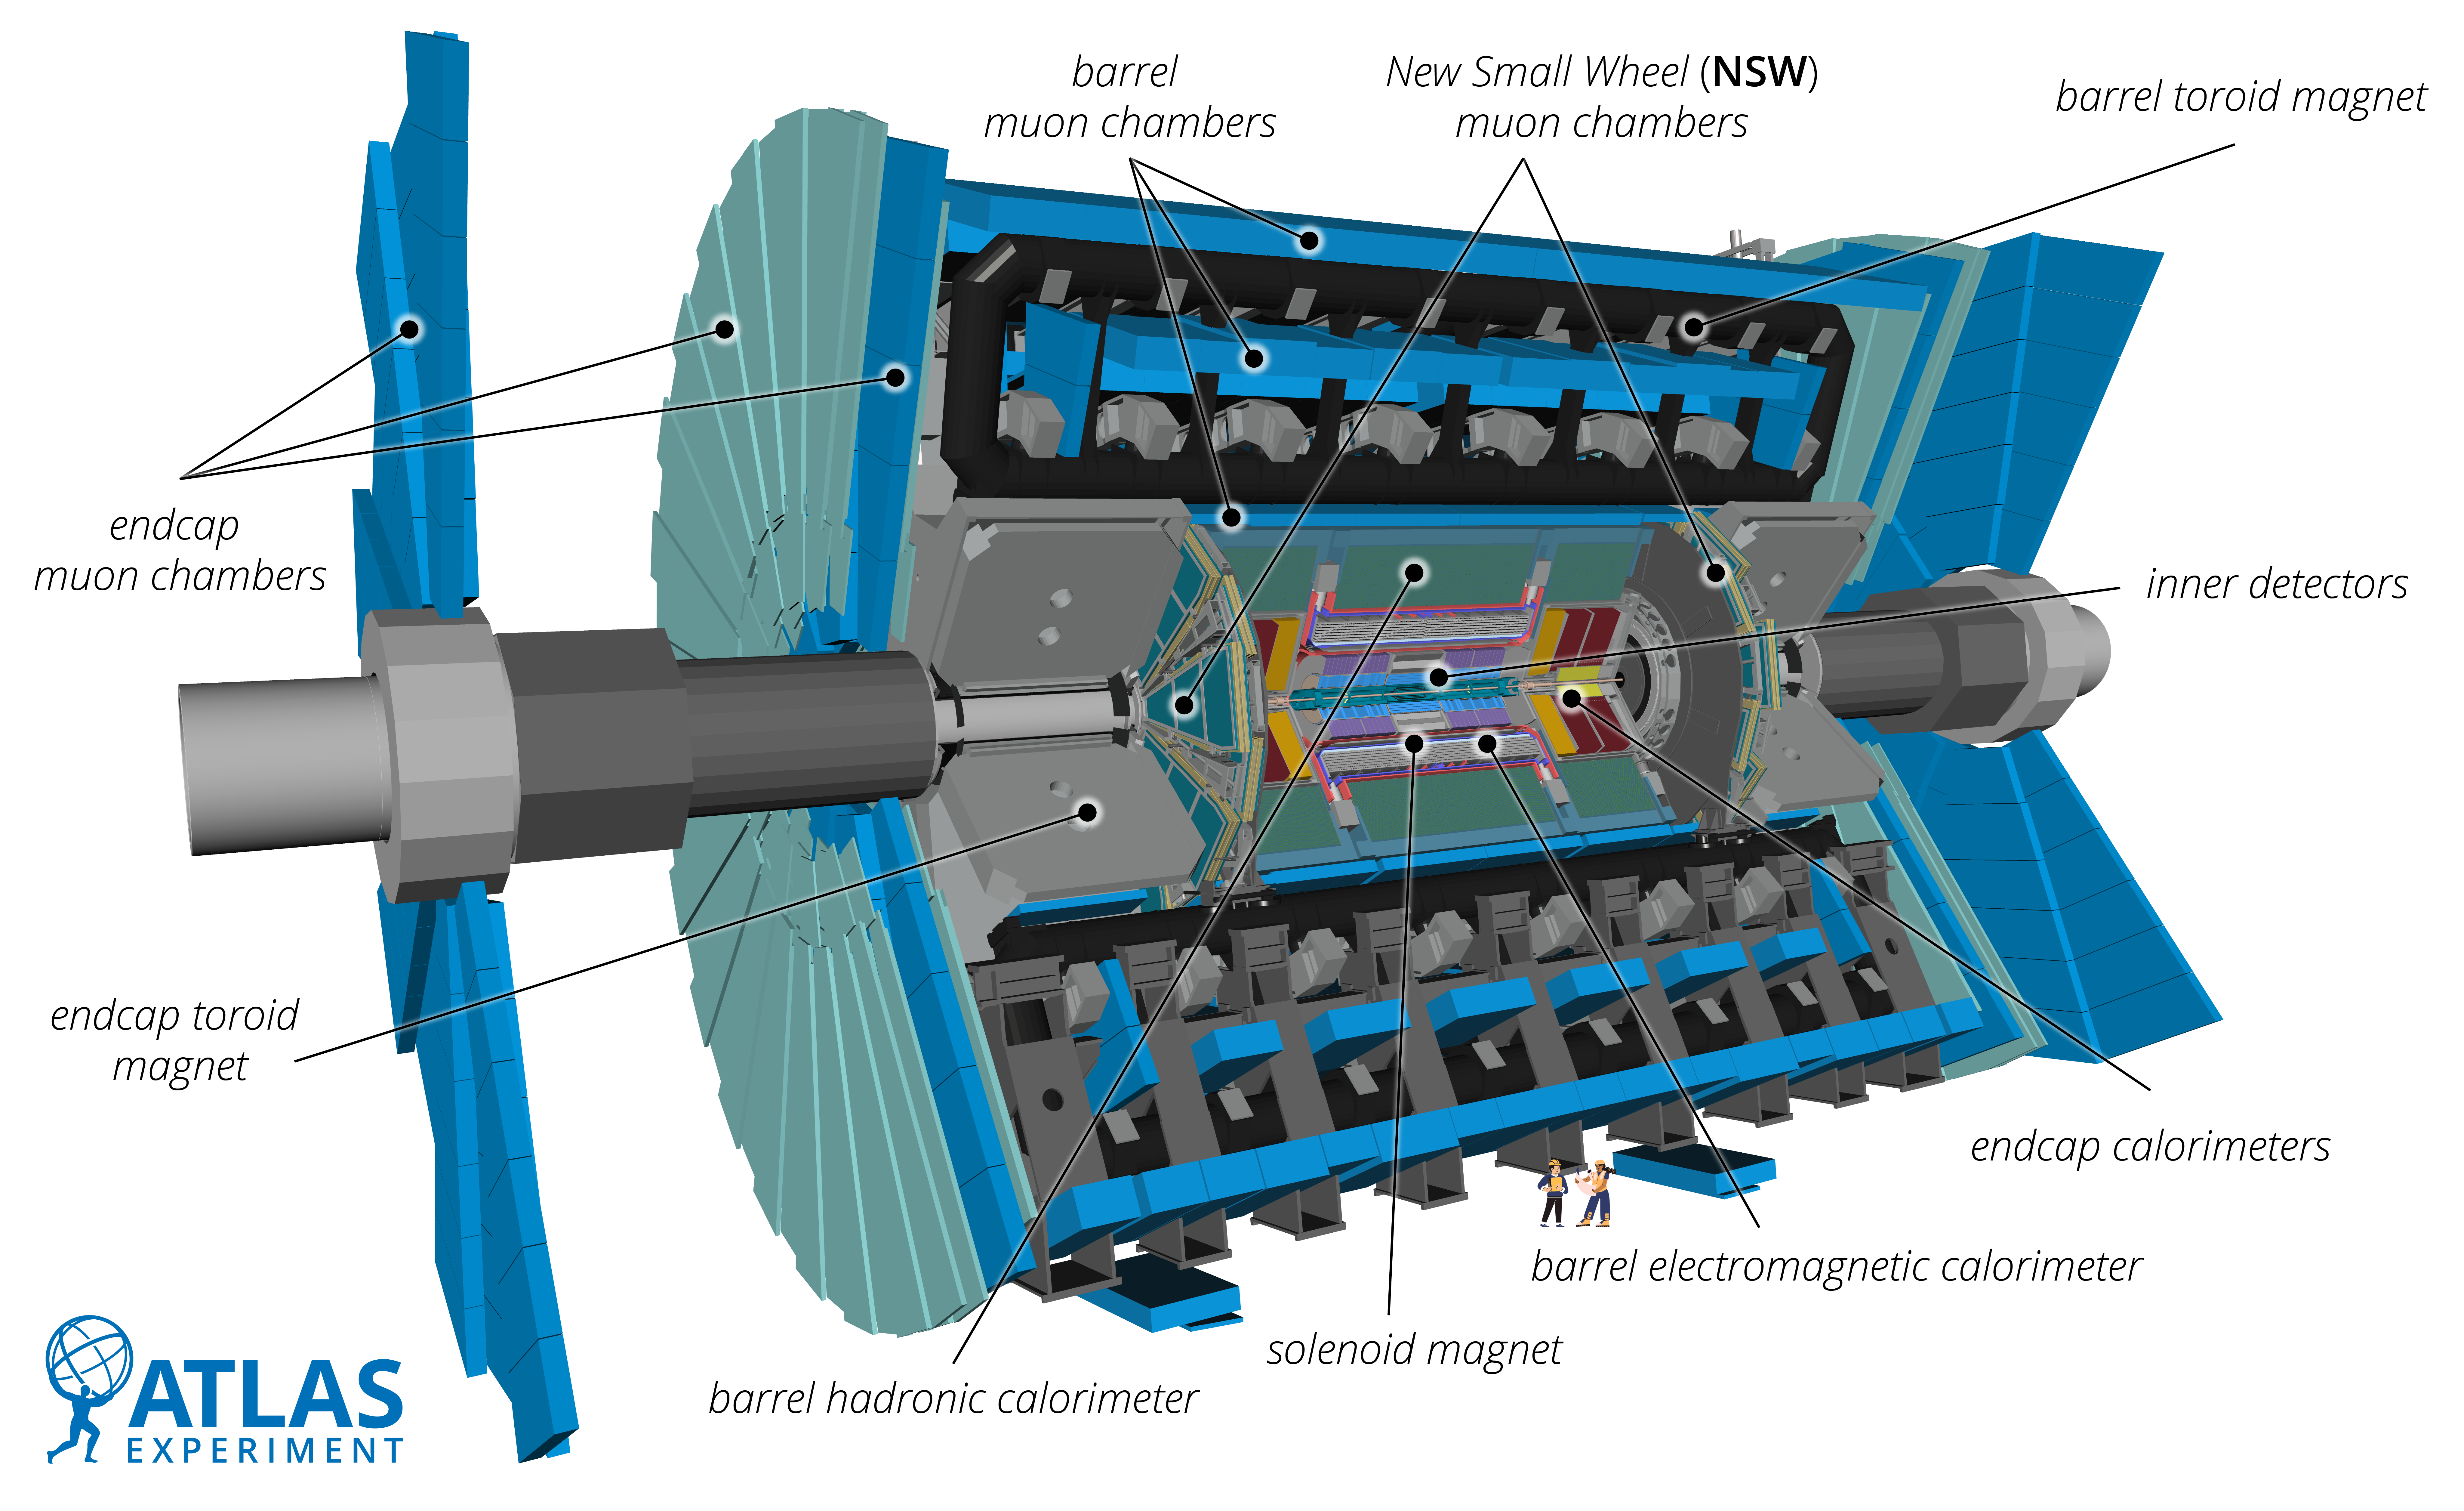
\includegraphics[width=0.8\linewidth]{3_experiment/atlas/ATLAS_full.png}
    \caption{Vista general del detector \ac{ATLAS} y de todos sus subdetectores, incluidos los sistemas añadidos durante el \ac{LS2}~\cite{ATLAS-Diagram}.}
    \label{fig:atlas:atlas:atlas}
\end{figure}

\ac{ATLAS} está construido en capas de subdetectores, cada uno de los cuales está diseñado para tener un papel diferente en la identificación y reconstrucción de las partículas producidas en las colisiones. \ac{ATLAS} proporciona una cobertura hermética alrededor del eje del haz, permitiendo la detección de todas las partículas cargadas generadas en las colisiones en el plano ortogonal al eje del haz. Esto es particularmente importante en las búsquedas de nueva física, que se basan en análisis de balances de momento en el plano ortogonal.

Está formado por múltiples capas, empezando por el componente más interno, el \acf{ID}, que permite reconstruir trazas cerca del tubo del haz. Alrededor del \ac{ID}, hay un solenoide superconductor que crea un campo magnético axial de \(\sim 2\) T para curvar las trazas de las partículas cargadas.
Tras este imán, hay un sistema de dos calorímetros: el \acf{ECAL} y el \acf{HCAL}. El primero se encarga de medir la energía cinética de fotones y electrones, y el segundo mide la energía de los jets.
Las partes más externas del \ac{ATLAS} están constituidas por el \acf{MS}, que proporciona la reconstrucción del momento de los muones que atraviesan las capas internas del detector. Entrelazadas con el \ac{MS}, hay un total de 8 bobinas toroidales que proporcionan un campo magnético total de 4 T para medir el momento de los muones. El campo magnético de los toroides se completa con los toroides en las regiones del end-cap, que también generan un campo magnético de hasta 4 T para los muones que salen en la dirección más próxima al haz.

% El trabajo conjunto de todos los componentes de \ac{ATLAS} permite reconstruir e identificar una gran variedad de partículas con gran precisión. En la \Tab{\ref{tab:atlas:atlas:expected_performance}}, adaptado de \Refn{\cite{ATLAS}}, se da una visión general de las capacidades de diseño de \ac{ATLAS} en términos de resolución de momento y energía.
% Aquí, la resolución está dada primero por un término estocástico, que mide la incertidumbre basada en la interacción de una partícula con el material, seguido de un término de ruido, que da cuenta de las incertidumbres debidas al ruido electrónico en el proceso de lectura.




% \begin{table}[ht!]
%     \caption{Rendimiento esperado del detector \ac{ATLAS}. Las unidades de \pt y \(E\) están en \gev. Extraído de \Refn{\cite{ATLAS}}}
%     \begin{tabular}{|l|c|c|c|}
%         \hline
%         \multirow{2}{*}{\textbf{Componente del detector}}    & \multirow{2}{*}{\textbf{Resolución requerida}}     & \multicolumn{2}{c|}{\textbf{Cobertura en $\eta$}}             \\\cline{3-4} 
%                                                         &                                                   & Offline               & Trigger                        \\ \hline
%         \ac{ID}                                        & \( \sigma_{\pt}/\pt = 0.05\%\pt \oplus 1\%    \)  & \( \pm 2.5 \)            &                                \\ \hline
%         \ac{ECAL}                                  & \( \sigma_{E}/E = 10\%/\sqrt{E} \oplus 0.7\%  \)  & \( \pm 3.2 \)            & \( \pm 2.5 \)                  \\ \hline
%         \ac{HCAL} (jets)                     &                                                   &                          &                                \\
%         $\quad$ barrel y end-cap                       & \( \sigma_{E}/E = 50\%/\sqrt{E} \oplus 3\%    \)  & \( \pm 3.2 \)            & \( \pm 3.2 \)                  \\
%         $\quad$ dirección forward                                  & \( \sigma_{E}/E = 100\%/\sqrt{E} \oplus 10\%  \)  & \( 3.1 < \abseta< 4.9 \) & \( 3.1 < \abseta< 4.9 \)       \\ \hline
%         \ac{MS}                               & \( \sigma_{\pt}/\pt = 10\%\) at \(\pt =1~\tev \)  & \( \pm 2.7 \)            & \( \pm 2.4 \)                  \\
%         \hline
%     \end{tabular}
%     \label{tab:atlas:atlas:expected_performance}
% \end{table}







\subsection{Sistema de coordenadas de ATLAS}

\begin{figure}[ht!]
    \centering
    \includegraphics[width=0.8\linewidth]{3_experiment/atlas/ATLAS_coordinates}
    \caption{Sistema de coordenadas de \ac{ATLAS}~\cite{ATLAS-Diagram}.}
    \label{fig:atlas:atlas:atlas_coordinates}
\end{figure}

El sistema de coordenadas utilizado en \ac{ATLAS}, que se muestra en \Fig{\ref{fig:atlas:atlas:atlas_coordinates}}, se utiliza en toda esta tesis y se describe brevemente a continuación~\cite{ATLAS}.
El origen del sistema de coordenadas está en el punto de interacción nominal, con el eje x positivo apuntando hacia el centro del \ac{LHC}. El plano x-y es perpendicular al eje del haz, definiendo el eje z. Hacia la superficie define el eje y positivo. Alrededor del eje del haz se define un ángulo azimutal $\phi$, y un ángulo polar $\theta$ es el ángulo desde el eje del haz. En lugar de $\theta$ se utiliza la rapidez $y$ que para objetos pesados tiene la forma:
\begin{equation}
    y = \frac{1}{2} \ln[(E+p_z)/(E-p_z)].
\end{equation}
Las diferencias en la rapidez son invariantes a \textit{boosts} a lo largo del eje del haz. Para objetos sin masa o relativistas ($m \ll \vb*{p}$) se utiliza en su lugar la pseudorapidez:
\begin{equation}
    \eta = -\ln(\tan(\theta/2)).
\end{equation}
Para cuantificar la distancia entre dos objetos, se define \DeltaR:
\begin{equation}
    \DeltaR = \sqrt{\Delta\phi^2 + \Delta\eta^2}
\end{equation}
El momento transverso y la energía se definen en el plano x-y, con el momento transverso dado como $\pt = \sqrt{p_x^2 +p_y^2}$.






\subsection{Detector Interno}
\label{subsec:atlas:atlas:id}

\begin{figure}[ht!]
    \centering
    \begin{subfigure}[t]{0.49\linewidth}
        \centering
        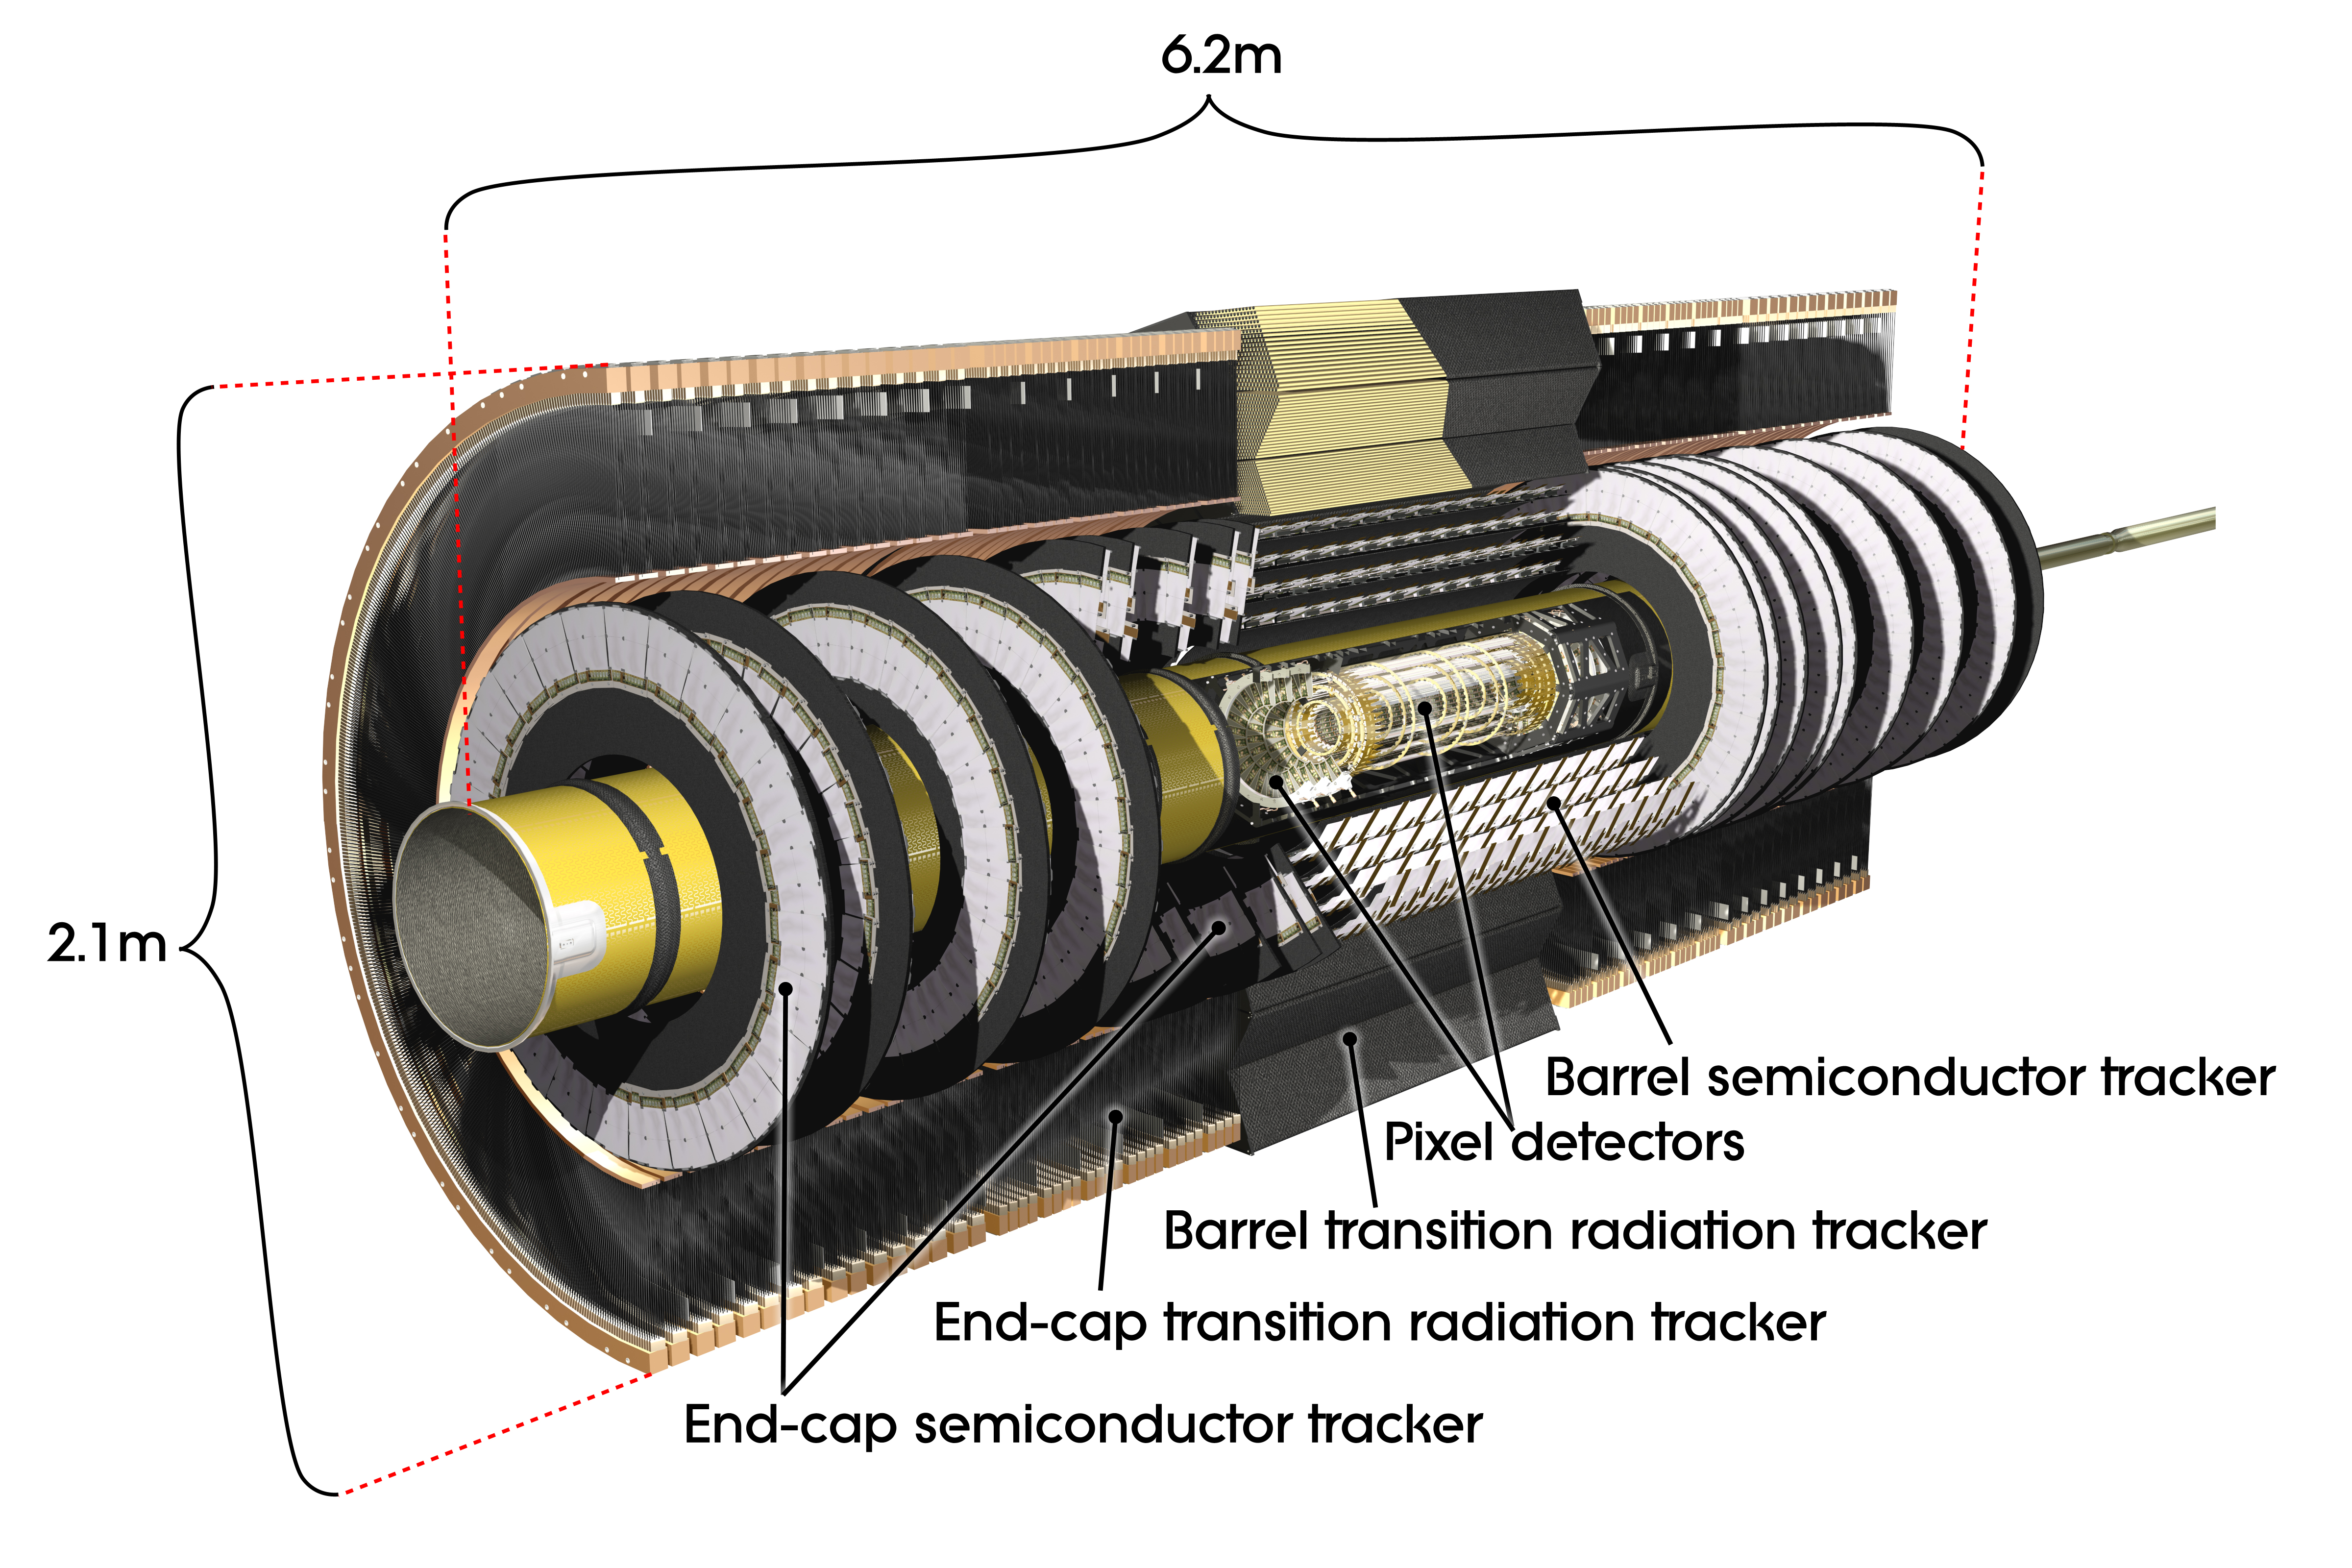
\includegraphics[width=\linewidth]{3_experiment/atlas/inner_detector.jpg}
        \caption{El \ac{ID} con todos sus submódulos en las regiones de barrel y end-cap.~\cite{ATLAS-InnerDetector}.}
        \label{fig:atlas:atlas:atlas_inner_detector:general}
    \end{subfigure}
    \hfill
    \begin{subfigure}[t]{0.49\linewidth}
        \centering
        \includegraphics[width=0.8\linewidth]{3_experiment/atlas/inner_detector_layers}
        \caption{Capas del \ac{ID} mostrando su distancia al haz~\cite{ATLAS-InnerDetector}.}
        \label{fig:atlas:atlas:atlas_inner_detector:layer_radius}
    \end{subfigure}
    \caption{Diagramas del \ac{ID} que muestran los diferentes submódulos, con sus correspondientes dimensiones.}
    \label{fig:atlas:atlas:atlas_inner_detector}
\end{figure}

El esquema de un corte transversal del \acf{ID} \cite{ATLAS-ID-TDR} se muestra en la \Fig{\ref{fig:atlas:atlas:atlas_inner_detector}}, resaltando la distancia de cada subsistema respecto al tubo del haz. La parte más interna del \ac{ID} se denomina \ac{IBL}, seguido de tres capas de detectores de píxeles. A 299 mm de distancia radial del tubo del haz, cuatro capas de módulos del \ac{SCT} se sitúan antes del \ac{TRT}, que amplía el tamaño total del \ac{ID} a un radio de 1082 mm. El \ac{ID} permite la reconstrucción de las trazas de partículas en un rango de $\abseta < 2.5$.


La función del \ac{ID} es la reconstrucción de las trazas de las partículas cargadas para determinar su carga y momento. Está inmerso en un campo magnético de 2 T generado por el sistema magnético del solenoide de \ac{ATLAS}, que curva las trayectorias de las partículas cargadas. El radio de curvatura es proporcional al momento de la partícula y su dirección distingue las cargas positivas de las negativas. Las trazas de las partículas detectadas permiten reconstruir los vértices de colisiones primarios, lo cual es importante para distinguir las colisiones de \textit{pile-up} (término que será descrito más adelante) de las colisiones de interés, y los vértices secundarios de decaimiento producidos por partículas de vida media larga, lo que es crucial para la identificación de, por ejemplo, mesones \(B\) o leptones \(\tau\). A continuación, se brinda una breve descripción de cada parte del \ac{ID}.


\paragraph{\acf{IBL}}
Después del Run-1, durante el \ac{LS1} en el período de 2013-2014, el sistema detector de píxeles fue sometido a mantenimiento y actualizaciones. Dentro de este conjunto de actualizaciones, una cuarta capa de píxeles a 3.3 cm de distancia del tubo del haz fue instalada~\cite{ATLAS-IBL-TDR,ATLAS-IBL-proceedings} y ha permitido mejoras significativas en la reconstrucción de vértices de interacción y la identificación de jets iniciados por quarks \(b\).


\paragraph{Detector de Píxeles}
La capa de píxeles más interna, el \ac{IBL}, está rodeada por tres capas de detectores de píxeles, dispuestas alrededor del tubo del haz~\cite{ATLAS-Pixel-DesignPerformance,ATLAS-Pixel-Performance-Proceedings}. El método de detección de partículas cargadas es la medición de cargas inducidas depositadas en una capa de silicio, producto de la ionización. La primera capa se encuentra a una distancia de 50.5 mm del centro del tubo del haz. Como se puede ver en la \Fig{\ref{fig:atlas:atlas:atlas_inner_detector:general}}, en la región del end-cap los detectores de píxeles consisten en 3 discos alrededor del tubo, aumentando la longitud del detector de píxeles del \ac{ID} a 1.4 m a lo largo del eje del haz. El detector de píxeles consta de un total de 1744 módulos de píxeles con un tamaño nominal de $50 ~\mu m \times 400 ~\mu m$ en el plano $(\phi, z)$, que comprenden más de 80 millones de canales de lectura.  
La parte de píxeles y \ac{IBL} del detector \ac{ATLAS} es crucial para la reconstrucción de trazas, ya que proporciona 4 puntos de medición (\textit{hits}) en todo el rango de cobertura de pseudorapidez ($|\eta| < 2.5.$).  

\paragraph{\acf{SCT}}
El detector de píxeles y \ac{IBL} se encuentran dentro de los módulos del \ac{SCT}~\cite{ATLAS-SCT}.  
Al igual que los módulos detectores de píxeles, los módulos del \ac{SCT} están basados en semiconductores, dispuestos en capas cilíndricas alrededor del tubo del haz en la región del barrel, formando discos en los end-caps. Dado que los módulos del \ac{SCT} sólo proporcionan una localización precisa a lo largo de un eje, se combinan dos módulos uno detrás de otro y rotados entre sí para obtener información espacial bidimensional. En el barrel hay cuatro capas y en los end-caps, nueve discos en cada lado (véase la \Fig{\ref{fig:atlas:atlas:atlas_inner_detector:general}}). Incluyendo los discos de los end-caps, el \ac{SCT} se extiende hasta $|z| < 2735~mm$.

\paragraph{\acf{TRT}}
La última parte del \ac{ID} es el \ac{TRT}~\cite{ATLAS-TRT-DesignPerformance}, el cual en la región barrel se extiende de 554 mm a 1082 mm de distancia radial. Este detector se compone de tubos detectores de 4 mm de diámetro, dispuestos en paralelo al tubo del haz en la región barrel, y radialmente en los end-caps. En el rango de $|\eta| < 2.0$, se sitúan tres anillos en el barrel y 18 unidades en los end-caps, proporcionando típicamente 36 impactos por traza. Los tubos están entrelazadas con fibras de polipropileno, que cuando las partículas las atraviesan, crean la radiación de transición. En el interior de los tubos hay un fino cable de tungsteno que recoge las cargas. El nivel de radiación y las cargas recogidas en cada tubo pueden utilizarse para discriminar entre electrones y piones cargados. El \ac{TRT} sólo ofrece información espacial en el plano $(R-\phi)$, y no se puede extraer información en la dirección z debido a la orientación de estos tubos. Hay un total de aproximadamente 50000 tubos en la región del barrel, mientras que en los end-caps se sitúan aproximadamente 250000 tubos.








\subsection{Calorímetros}

\begin{figure}[ht!]
    \centering
    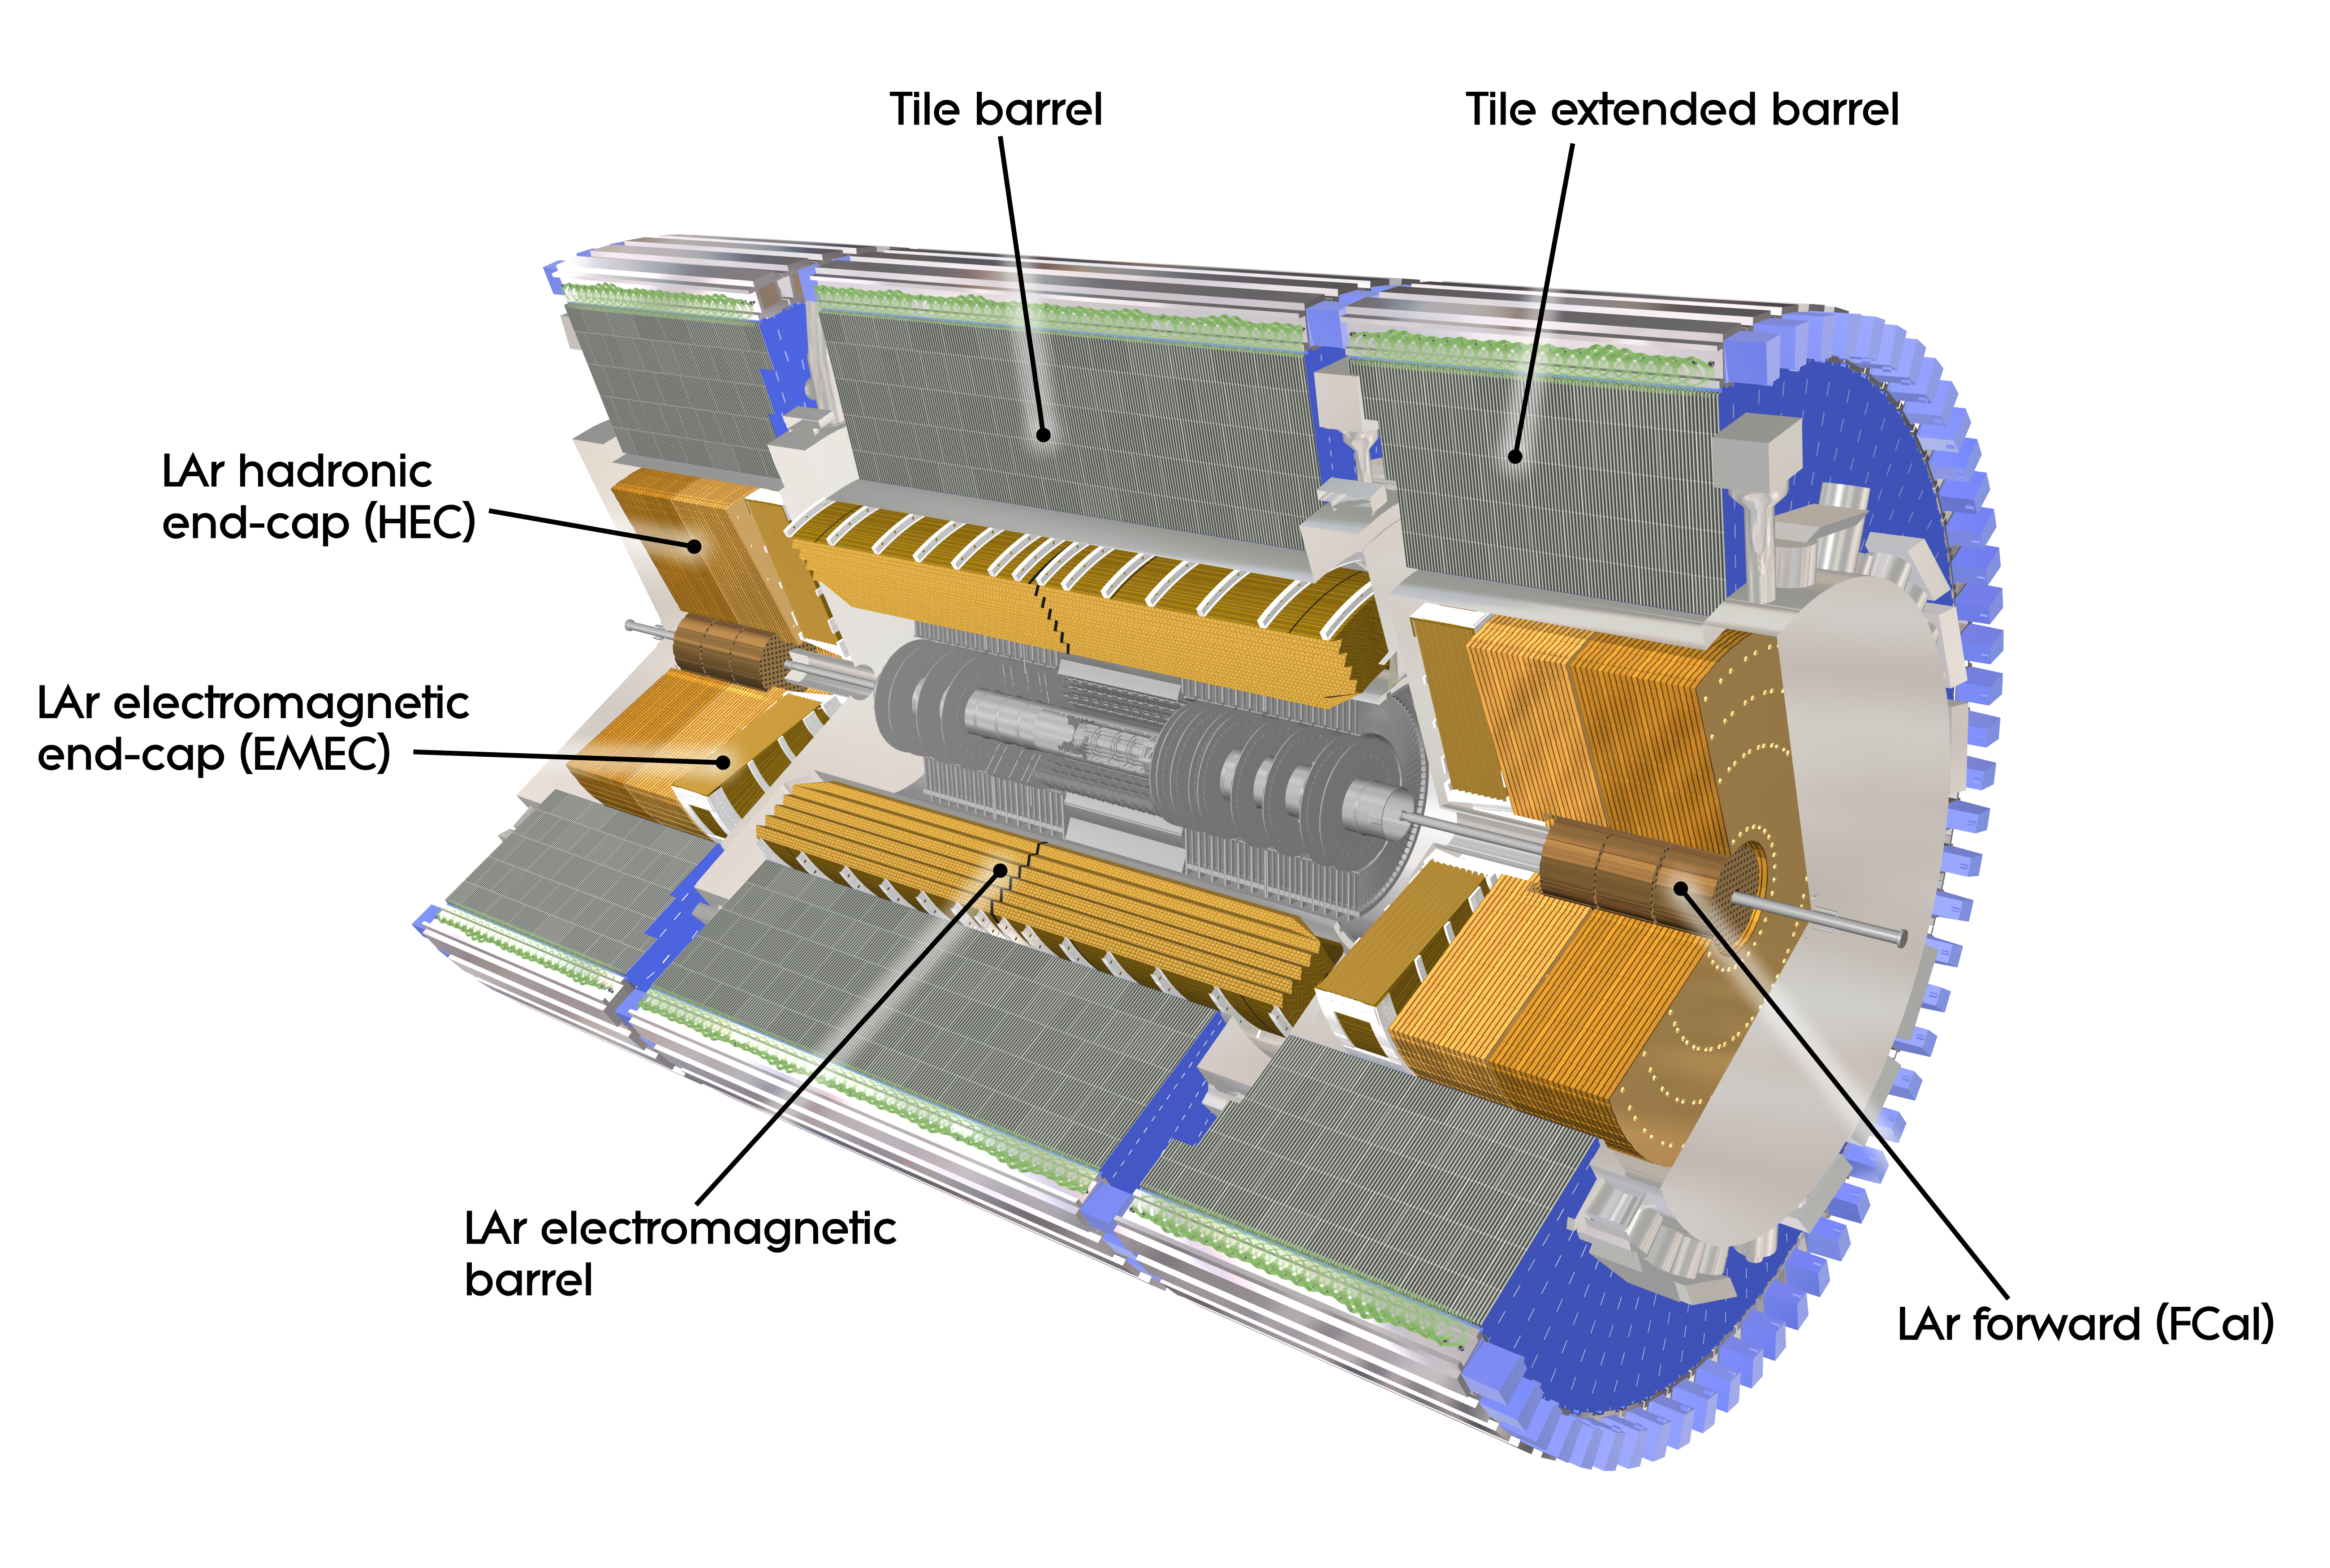
\includegraphics[width=0.8\linewidth]{3_experiment/atlas/calorimenters.jpg}
    \caption{Sistema de calorímetros de \ac{ATLAS}, mostrando el \acf{ECAL} y el \acf{HCAL}~\cite{ATLAS-Calorimeter-Diagram}.}
    \label{fig:atlas:atlas:atlas_calorimeters}
\end{figure}

El sistema \ac{ID} está rodeado por dos calorímetros: el \acf{ECAL} y el \acf{HCAL}, como se muestra en la \Fig{\ref{fig:atlas:atlas:atlas_calorimeters}}. Estos calorímetros están diseñados para medir la energía y la posición de las partículas incidentes, a través de la energía depositada por las cascadas de partículas secundarias producidas por las incidentes. Cubre todo el rango \(\phi\) y hasta el \(\abseta<4.9\), con una granularidad más fina en la región que coincide con el \ac{ID}.
El sistema de calorímetro permite discriminar entre fotones y electrones de hadrones (jets). Además, permite medir el desequilibrio energético (gracias a su cobertura total y hermiticidad) y proporciona al sistema de trigger la información necesaria para la selección de eventos.

Ambos calorímetros son denominados calorímetros de muestreo, con capas alternas de material absorbente y activo. La capa absorbente desencadena una lluvia de partículas consecutivas con el material detector, la capa activa detecta la señal.
El desarrollo de la lluvia y sus propiedades son de vital importancia para la identificación de las partículas, como se verá más adelante.
Dos magnitudes importantes en relación con los calorímetros son la longitud de radiación, $X_0$, y la longitud de interacción $\lambda$. La longitud de radiación se refiere a la distancia después de la cual la energía de una partícula (electrones por ejemplo) se ha reducido a \(1/e\) de su energía inicial. La longitud de interacción describe el camino libre medio antes de que se produzca una interacción hadrónica.

La resolución de diseño del sistema sobre la energía calorimétrica viene dada por
\begin{equation}
    \frac{\sigma(E)}{E} = 
    \frac{a}{\sqrt{E}} \oplus b \oplus \frac{c}{E}
\end{equation}
donde \(\oplus\) significa que los términos se suman en cuadratura. El término estocástico \(\frac{a}{\sqrt{E}}\) está relacionado con las fluctuaciones en los desarrollos de la lluvia, el término constante \(b\) tiene en cuenta las inhomogeneidades del detector, y el último término está asociado con el ruido electrónico y es proporcional a \(\frac{1}{E}\). El valor de los coeficientes \(a\) y \(b\) depende de los objetos incidentes. Para el caso de los electrones en el \ac{ECAL}, \(a\sim 10\%~\gev^{1/2}\) y \(b~\sim 0.7\%\), mientras que los de los piones cargados en el centro del detector son \(a~\sim50\%~\gev^{1/2}\) y \(b\sim5\%\) \cite{ATLAS-Calorimeters-PerformanceRun2}.



\subsubsection{\acf{ECAL}}
\label{subsubsec:atlas:atlas:cals:ecal}

El \ac{ECAL} está especializado en la detección de electrones, positrones y fotones, que depositan su energía en lluvias relativamente densas: electrones energéticos que irradian fotones Bremsstrahlung, mientras que los fotones energéticos se convierten en pares electrón-positrón al atravesar el material denso.
El material absorbente está hecho de plomo (Pb) con láminas de acero inoxidable, mientras que el \ac{LAr} se utiliza como material activo con electrodos de cobre y kaptón para la lectura.


El calorímetro tiene una geometría de acordeón que proporciona una simetría completa \(\phi\) sin fisuras azimutales.
Está dividido en dos medios barriles que cubren la región central del detector (\(\abseta<1.475\)), con un pequeño hueco (4 mm) en $z = 0$ y una tapa final a cada lado del haz (\(1.375<\abseta<3.2\)).
La región de transición entre el barrel y end-cap se denomina región \textit{crack}, y la mayoría de los análisis físicos que utilizan el \ac{ECAL} requieren que los fotones y electrones se encuentren fuera de ella.
Además el \ac{LAr} se utiliza para las tapas de los calorímetros hadrónicos, así como en el \acf{FCAL} ($3.1 < \eta < 4.9$).

El grosor de \ac{ECAL} es superior a 22 longitudes de radiación (\(X_0\)) en la región del barrel, mientras que es superior a \(24 X_0\) en la región de end-caps. En el caso de los fotones, la distancia a la que la energía baja a \(1/e\) es de \(9/7 X_0\), por lo que toda la energía electromagnética del fotón se deposita en el \ac{ECAL}, y sólo una pequeña parte llega al \ac{HCAL}.

El modo de medición es el siguiente. Las partículas incidentes interactúan con el medio absorbente (Pb), iniciando una lluvia de partículas cargadas y neutras. Las partículas cargadas ionizan el \ac{LAr} y los electrodos recogen los electrones producidos en el proceso de ionización. La señal total del medio activo es entonces proporcional a la energía real total de la partícula incidente.

\begin{figure}[ht!]
    \centering
    \includegraphics[width=0.8\linewidth]{3_experiment/atlas/ecal_cells}
    \caption{Segmento del \ac{ECAL} mostrando la disposición de las capas y celdas del calorímetro. Además, se muestran las dimensiones de las celdas en cada capa~\cite{ATLAS}.}
    \label{fig:atlas:atlas:cals:ecal:ecal_cells}
\end{figure}

\begin{figure}[ht!]
    \centering
    \includegraphics[width=0.46\linewidth]{3_experiment/atlas/ecal_radiation_lengths1}
    \includegraphics[width=0.46\linewidth]{3_experiment/atlas/ecal_radiation_lengths2}
    \caption{Longitudes de radiación en función de \abseta para cada capa del \ac{ECAL}~\cite{ATLAS}.}
    \label{fig:atlas:atlas:cals:ecal:ecal_radiation_length}
\end{figure}

Dentro de la región aceptada para las medidas de precisión (\(\abseta<2.5\) excluyendo el crack), el \ac{ECAL} se segmenta en tres capas longitudinales, mostradas en la \Fig{\ref{fig:atlas:atlas:cals:ecal:ecal_cells}}.
La primera capa consiste en bandas de granularidad fina (también llamada \textit{strip layer}) que ayuda a discriminar entre fotones aislados y pares de fotones espacialmente cercanos procedentes de decaimientos \(\pizero\to\gamma\gamma\). Esta capa tiene un espesor constante de \(\sim 6 X_0\) en función de \(\eta\) (véase la \Fig{\ref{fig:atlas:atlas:cals:ecal:ecal_radiation_length}}), y proporciona una medida precisa de \(\eta\).
Para los fotones y electrones de alta energía, la mayor parte de su energía se recoge en la segunda capa, que tiene una granularidad lateral de \(0.025 \times 0.025\) en \((\eta, \phi)\) y un espesor de \(\sim 24 X_0\).
La tercera capa recoge la energía depositada por las colas de la lluvia electromagnética, con un espesor que varía entre 2 y 12 \(X_0\).
También hay un \textit{presampler} (no se muestra en las figuras), que cubre la región \(\abseta<1.8\) que mejora la medición de la energía para las partículas que comienzan la lluvia antes de entrar en el calorímetro.




\subsubsection{\acf{HCAL}}



Tres capas de calorímetro hadrónico rodean el \ac{ECAL} y proporcionan discriminación adicional para electrones y fotones al medir la energía hadrónica. El \ac{HCAL} se extiende en pseudorapidez hasta \(\abseta<4.9\), permitiendo cubrir prácticamente la totalidad del ángulo sólido desde el punto de interacción. En la región del barrel (\(\abseta<1.7\)) se encuentra el primer calorímetro, el \textit{Tile calorimeter}, un calorímetro de muestreo que utiliza acero como material absorbente y tejas centelladoras como material activo~\cite{ATLAS-Tile-TDR}. Está dividido en dos partes: \(\abseta<1.0\) y \(0.8<\abseta<1.7\). Las tejas centelleadoras están dispuestas de una forma periódica y están conectadas a una fibra óptica que transporta la luz producida por las partículas que pasan a un tubo fotomultiplicador. Este arreglo se extiende, en \(R\), de 2.28 a 4.25 m. En la región del end-cap (\(1.5<\abseta<3.2\)) hay un calorímetro de muestreo hadrónico, el \acf{HEC}, con placas de cobre como absorbente y argón líquido como material activo. Cada lado del endcap consiste en dos ruedas, una detrás de la otra con las placas planas de Cu dispuestas perpendicularmente al eje del haz, con un radio de 2.3 m. Finalmente está el \ac{FCAL}, un calorímetro de muestreo que extiende la cobertura del sistema hasta \(\abseta<4.9\), coaxial al eje del haz y situado a 4.7 m a cada lado del punto de interacción. El material principal de los módulos es el \ac{LAr} (con cobre o tungsteno), y aunque no se utiliza para mediciones de precisión, proporciona información para el cálculo de la energía transversa faltante y la reconstrucción de jets en regiones muy cercanas al eje del haz.

El \ac{HCAL} tiene un espesor superior a \(7.7~\lambda\) en la región del barrel (\(9.7~\lambda\) en total si se cuenta el \ac{ECAL}). Análogamente a la longitud de radiación mencionada para el \ac{ECAL}, se puede definir la longitud de interacción hadrónica como la distancia media a lo largo de la cual la energía de un hadrón se reduce a \(1/e\) de su energía inicial. Así, toda la energía con la que los hadrones llegan al \ac{HCAL} se deposita allí.





\subsection{\acf{MS}}

\begin{figure}[ht!]
    \centering
    \includegraphics[width=0.6\linewidth]{3_experiment/atlas/muon_detector}
    \caption{Diagrama del \acf{MS}~\cite{ATLAS}.}
    \label{fig:atlas:atlas:muon_spectrometer:muon_spectrometer}
\end{figure}

Los muones de alto \pt generados en el punto de interacción tienen un poder de penetración muy elevado y son poco interactivos. Por lo tanto, el \ac{MS} \cite{ATLAS-Muon-TDR} está situado en la parte más externa del detector \ac{ATLAS}, insertado dentro del campo magnético de 4 T generado por los imanes toroidales del barrel y end-caps, y está diseñado para obtener medidas de posición y momento con alta precisión de los muones de alto \pt en un rango de \abseta de \(\abseta<2.7\). Se trata del mayor subdetector y el que da a \ac{ATLAS} su tamaño. Este subdetector se muestra en la \Fig{\ref{fig:atlas:atlas:muon_spectrometer:muon_spectrometer}}, destacando los subsistemas.

El \ac{MS} se compone de diferentes tipos de cámaras de detección (véase la \Fig{\ref{fig:atlas:atlas:muon_spectrometer:muon_spectrometer}}). Los \acp{MDT} son responsables de la mayoría de las medidas de precisión y cubren el rango de pseudorapidez hasta \(\abseta<2.7\). Funcionan de forma similar al \ac{TRT}, con tubos llenos de un gas ionizante y un ánodo central que recoge los electrones producidos, y el tiempo de deriva está asociado a la distancia a la traza dejada por la partícula. En la región del endcap se encuentran las \acp{CSC} que tienen una alta resolución espaciotemporal y una cobertura de \(\abseta>2.0\). Estas cámaras funcionan midiendo la carga depositada en un ánodo como resultado de la cascada de electrones creada cerca de él. Las \acp{RPC} proporcionan una estimación rápida del momento de los muones a nivel de trigger con una cobertura de \(\abseta<1.05\)\footnote{Durante el \ac{LS2}, la capa del end-cap ma\'s interna ha sido reemplazada por las \acp{NSW}~\cite{ATLAS-NSW}. Presenta MicroMegas como rastreadores de precisión ya que proporcionan un mejor rendimiento a las altas tasas esperadas en las futuras operaciones del LHC.}. Las \acp{RPC} miden la descarga entre dos placas resistivas paralelas sometidas a una elevada diferencia de potencial, siguiendo la ionización del volumen de gas interno causada por el paso de muones energéticos. Por último, en la región del endcap, se encuentran los \acp{TGC}, de función similar a los \acp{CSC}. También proporcionan información al sistema de trigger en esta región y tienen una cobertura de \(\abseta<2.4\).

Si los hits en el \ac{ID} y el \ac{MS} se pueden asociar a un solo muón, se obtiene una muy buena resolución del momento de hasta
\begin{equation}
    \frac{\sigma(\pt)}{\pt} = 
    0.02\% \cdot \pt~[\gev] \oplus 2\%,
\end{equation}
la cual se degrada si sólo se identifica una traza en uno de los dos sistemas.






\subsection{El sistema de Trigger}



El sistema de trigger de \ac{ATLAS}~\cite{ATLAS-Trigger-Performance-2010,ATLAS-Trigger-Performance-2015,ATLAS-Trigger-Performance-Run2} utiliza información del detector para rechazar eventos que no son de interés para el programa de \ac{ATLAS} (colisiones \textit{soft}, por ejemplo), reduciendo la frecuencia de eventos de 40 MHz (frecuencia de cruce de bunches mencionada en la \Sect{\ref{sec:atlas:LHC}}) a alrededor de 1.5 kHz. Es necesario enfatizar aquí el papel central del sistema de trigger para el correcto funcionamiento de todo el experimento, siendo el responsable de decidir qué eventos se almacenan para su posterior análisis, que podría llevar, por ejemplo, a un descubrimiento. Para lograr tal reducción en la frecuencia de eventos y, al mismo tiempo, tener una alta eficiencia en la selección de los de interés, el sistema de trigger se compone de dos niveles consecutivos capaces de realizar una identificación de partículas cada vez más compleja; un primer nivel de trigger basado en hardware, el \acf{L1}, y luego un trigger de alto nivel basado en software, el \acf{HLT}. Cada nivel permite analizar los eventos con mayor detalle, aumentando la precisión de los criterios de selección y la complejidad de los algoritmos utilizados.


\subsubsection{\acf{L1}}

La decisión del trigger comienza con el \ac{L1}, basado en hardware~\cite{ATLAS-L1Trigger}, que identifica lo que se conoce como \ac{ROI}. La \ac{ROI} consiste en celdas vecinas en los \ac{ECAL} y \ac{HCAL}, y se define a partir de la posición en el calorímetro de cada objeto encontrado en un evento potencialmente interesante, que se extiende como un cono desde el punto de interacción a lo largo del detector.
En cuanto a los muones, toma la información leída por el \ac{MS}, más concretamente por el \ac{TGC} y el \ac{RPC}, y permite obtener una estimación rápida del \pt del muón.
El \ac{L1} también tiene una componente que permite tener en cuenta los requisitos topológicos, como las selecciones de masa invariante y las medidas de distancia, denominado el \ac{L1Topo}.

El diseño del \ac{L1} permite tener una aceptabilidad en el rango de \(\abseta<2.5\) para electrones, fotones, muones y taus, hasta \(\abseta<3.2\) para jets, y \(\abseta<4.9\) para el cálculo del momento transverso faltante.
Utilizando las \acp{ROI}, el trigger \ac{L1} debe tomar la decisión de guardar o descartar el evento, reduciendo la tasa de eventos de 40 MHz a menos de 100 kHz en aproximadamente \(2.5~\mu s\), tiempo determinado en parte por el tamaño limitado de los buffers de memoria y en parte por el tiempo que tardan los muones producidos en el evento en llegar al \ac{MS}. Esta decisión final la toma el \ac{CTP}, y luego pasa las \acp{ROI} al siguiente nivel de trigger: el \ac{HLT}.



\subsubsection{\acf{HLT}}


Cuando un evento es aceptado por el \ac{L1}, el \ac{HLT}~\cite{ATLAS-HLTTrigger} ejecuta una secuencia de algoritmos a partir de las \acp{ROI} definidas por el \ac{L1}, y permite reducir la tasa de eventos que se almacena a 1.5 kHz en 0.2 s.
La reconstrucción e identificación de partículas candidatas en el \ac{HLT} se evalúa en una secuencia de pasos donde se aplican diferentes algoritmos.
Si la selección falla en un determinado paso, los pasos siguientes ya no se ejecutan para ahorrar tiempo de ejecución.
En el \ac{HLT}, los algoritmos se agrupan en conjuntos de algoritmos de reconstrucción rápida que se ejecutan en primer lugar y, a continuación, se ejecuta un conjunto de algoritmos de reconstrucción de precisión similares a los utilizados \textit{offline}.
Los algoritmos de reconstrucción rápida utilizan la información del calorímetro y de las trazas del \ac{ID} sólo dentro de la \ac{ROI} para realizar la selección e identificación de candidatos, y llevar a cabo el rechazo del fondo lo más rápido posible.
Si la partícula candidata supera los criterios definidos por la selección de reconstrucción rápida, se ejecutan los algoritmos de selección de precisión. Estos tienen acceso a la información del detector fuera de la \ac{ROI}, con la máxima granularidad e incluyendo detalles sobre la calibración energética del calorímetro, la alineación del subdetector y el mapeo del campo magnético.

La secuencia exacta y el tipo de algoritmos considerados en el \ac{HLT} se definen en el \textit{menu} del trigger. Esto comprende una base de datos de triggers, cada uno de los cuales define una secuencia de algoritmos y los requisitos de estos algoritmos para que un evento pase el \ac{HLT}.

Los requisitos de trigger se diseñan de forma tal que la tasa global del \ac{HLT} no supere 1 kHz. En algunos casos, incluso la reducción de la tasa de eventos conseguida mediante los algoritmos del \ac{HLT} para los requisitos de trigger deseados, como los trigger para objetos con bajo momento, es demasiado alta. Para mantener la tasa general del \ac{HLT} por debajo de 1 kHz en estos casos, los triggers pueden seguir incluyéndose en el menú, pero con una preescala. Un preescalado es un escalado artificial del trigger, que sólo acepta la N-ésima decisión de trigger si el factor de preescalado es N. Esto permite que los triggers con una alta tasa sigan recogiendo eventos.

Los algoritmos del \ac{HLT} se ejecutan en aproximadamente 40.000 núcleos de CPU. Además, la construcción parcial de eventos se utiliza para análisis a nivel de trigger, para el monitoreo del detector y las calibraciones del subsistema detector. Finalmente, los eventos aceptados por el \ac{HLT} se almacenan y se distribuyen, disponibles \textit{offline} para cualquier estudio o análisis.






\FloatBarrier
\section{Toma de datos durante el Run-2}
\label{sec:atlas:runs}


El funcionamiento del \ac{LHC} se organiza en distintos períodos conocidos como \textit{runs}.
% Cada run suele durar varios años y se caracteriza por condiciones experimentales específicas, como la energía a la que colisionan los protones y la intensidad de los haces.
Desde su puesta en marcha, se pueden distinguir los siguientes runs: Run-1 (2010-2013) operó a energías de colisión de hasta 8 TeV, Run-2 (2015-2018) a 13 TeV, y Run-3 (2022-presente) a 13.6 TeV. Cada período de toma de datos, una vez que el \ac{LHC} anuncia haces estables, se divide en \ac{LB} de aproximadamente dos minutos. En cada \ac{LB}, la luminosidad instantánea es prácticamente constante y las condiciones del haz son estables. Debido a la alta complejidad del \ac{LHC} y del detector \ac{ATLAS}, se espera que haya ineficiencias en los detectores y subdetectores y/o en la cadena de adquisición de datos. Durante cada run, cada parte del \ac{ATLAS} es monitoreada y cualquier falla o problema es registrado, incluyendo componentes inactivos, o problemas en el haz del \ac{LHC}.

Para garantizar la alta calidad de los datos, libres de defectos significativos, los \ac{LB} y los rangos dentro de ellos que superan todos los criterios de calidad se compilan en \ac{GRL}. Las listas se elaboran y distribuyen de forma centralizada, con el fin de proporcionar a cualquier grupo de \ac{ATLAS} la misma colección de \acp{LB}. Dado que durante los períodos de tomas de datos están disponibles diferentes partes del detector (en un run óptimo, todos los subdetectores están disponibles), hay múltiples \acp{GRL} disponibles para utilizar. Cada análisis, entonces, selecciona qué \ac{GRL} utilizar dependiendo de su tolerancia a las fallas de los subdetectores.

La presente tesis utiliza datos recolectados por \ac{ATLAS} de colisiones \pp del \ac{LHC} durante el Run-2 (2015-2018), a una energía del centro de masa de \(\sqrt{s} = 13~\tev\). Durante este run, el \ac{LHC} entregó un total de \(156~\ifb\), de los cuales \ac{ATLAS} recolectó \(147~\ifb\). La luminosidad integrada total disponible para análisis de física es de \(140.07~\ifb\)\footnote{Las primeras medidas y \ac{GRL} iniciales sólo brindaban un total de \(139~\ifb\) disponibles para análisis}, como se ve en la \Fig{\ref{fig:atlas:runs:lumi_run2}}. La incertidumbre en la luminosidad integrada combinada para el Run-2 es de \(0.83\%\)~\cite{ATLAS-Lumi-Run2}, obtenida usando el detector LUCID-2~\cite{ATLAS-LUCID2}.
Hasta el momento, combinando los años 2022, 2023 y 2024 de toma de datos del Run-3, se recogieron 159 \ifb de datos, mostrados en la \Fig{\ref{fig:atlas:runs:lumi_run3}}~\cite{ATLAS-Lumi-Run3-2022,ATLAS-Lumi-Run3-2023}.

\begin{figure}[ht!]
    \centering
    \begin{subfigure}[h]{0.46\linewidth}
        \centering
        \includegraphics[width=\linewidth]{3_experiment/lhc/DeliveredLuminosityRun2}
        \caption{Run-2 (2015-2018)}
        \label{fig:atlas:runs:lumi_run2}
    \end{subfigure}
    \hfill
    \begin{subfigure}[h]{0.46\linewidth}
        \centering
        \includegraphics[width=\linewidth]{3_experiment/lhc/DeliveredLuminosityRun3}
        \caption{Early Run-3 (2022-2024)}
        \label{fig:atlas:runs:lumi_run3}
    \end{subfigure}
    \caption{Luminosidad entregada por el \ac{LHC} y recolectada por \ac{ATLAS} durante el Run-2~\cite{ATLAS-Lumi-Run2} y el Run-3. En el caso de Run-2, también se muestra la fracción de datos recolectados que son útiles para análisis de física.}
    \label{fig:atlas:runs:lumi}
\end{figure}

Otro concepto importante en la adquisición de datos en \ac{ATLAS} es el \textit{pileup}, que se produce cuando las partículas producidas en más de una colisión \pp llegan al detector al mismo tiempo, o más generalmente, cuando las señales se solapan de forma que no pueden separarse. Cuando colisionan haces de protones, la probabilidad de que se produzca una interacción es proporcional a la densidad de partículas, o mejor, al flujo de partículas, que se expresa mediante la luminosidad instantánea. El número real de colisiones de partículas que tienen lugar cuando dos haces se cruzan es una variable aleatoria que sigue una distribución de Poisson. Para luminosidades bajas, en la mayoría de los cruces de haces no se produce ninguna colisión, pero para luminosidades instantáneas altas, en la mayoría de los cruces se producen muchas colisiones simultáneas entre partículas. Dependiendo del subdetector y del tipo de medida, puede o no ser posible distinguir entre partículas procedentes de diferentes interacciones simultáneas. Es lo que se denomina como \textit{in-time pileup}. Por el contrario, el \textit{out-of-time pileup} incluye los efectos que surgen cuando el tiempo que el detector necesita para volver a su estado de espera es mayor que el tiempo entre cruces de haces. Una medida cuantitativa del pileup y de la actividad de eventos es el valor medio de interacciones inelásticas \pp por bunch-crossing, \avgmu.

Las luminosidades instantáneas máximas se multiplicaron por cuatro a lo largo de los cuatro años del Run-2, resultando en un aumento de \avgmu desde 10 hasta 60, como se muestra en la \Fig{\ref{fig:atlas:runs:pileup_run2}}. Para el Run-3, el pileup aumentó drásticamente hasta valores de 57 para el año 2024, aumentando en promedio hasta 52 interacciones por bunch-crossing, mostradas en la \Fig{\ref{fig:atlas:runs:pileup_run3}}.

\begin{figure}[ht!]
    \centering
    \begin{subfigure}[h]{0.46\linewidth}
        \centering
        \includegraphics[width=\linewidth]{3_experiment/lhc/PileupConditionsRun2.png}
        \caption{Run-2}
        \label{fig:atlas:runs:pileup_run2}
    \end{subfigure}
    \hfill
    \begin{subfigure}[h]{0.46\linewidth}
        \centering
        \includegraphics[width=\linewidth]{3_experiment/lhc/PileupConditionsRun3.png}
        \caption{Run-3}
        \label{fig:atlas:runs:pileup_run3}
    \end{subfigure}
    \caption{Distribución del número de interacciones por bunch-crossing durante Run-2 (izquierda) y Run-3 (derecha).}
    \label{fig:atlas:runs:pileup}
\end{figure}
\chapter{Reconstrucci\'on e identificaci\'on de objetos f\'isicos}
\label{ch:objects}
\epigraph{\emph{“Champions keep playing until they get it right.”}}{Billie Jean King}


Las partículas producidas en cada colisión y los productos de sus decaimientos, interactúan con el detector de una manera particular según su naturaleza. La información recogida por todos los subdetectores de \ac{ATLAS} permite reconstruir e identificar los objetos físicos presentes en cada evento aceptado por el sistema de trigger (selecci\'on \textit{online}). En este cap\'itulo se describen los algoritmos de reconstrucción e identificación \textit{offline}, que se lleva una vez que los eventos han sido aceptados por el trigger y almacenados.. La reconstrucción se realiza evento por evento, y se lleva a cabo del mismo modo para los eventos recolectados por el detector \ac{ATLAS} y para los eventos simulados con \acf{MC}. A continuación, se da un breve resumen de la reconstrucción offline y la identificación de los objetos utilizados en esta tesis.




\section{Reconstrucci\'on de trazas y v\'ertices}

En un evento con alto pileup, puede haber del orden de 1000 partículas cargadas pasando por el detector \ac{ATLAS}. La información del \ac{ID} (\Sect{\ref{subsec:atlas:atlas:id}}) se utiliza para reconstruir las trayectorias de las partículas cargadas, denominadas tazas (\textit{tracks}).

Dado que el \ac{ID} es el detector más cercano al haz y está compuesto por material mínimamente ionizante con una granularidad elevada, este detector desempeña el papel principal en la reconstrucción de trazas. Estas, permiten calcular el momento y la trayectoria de las partículas cargadas, dado que dejan una se\~nal en las diferentes capas del \ac{ID}. Adem\'as, como el campo solenoidal dentro del \ac{ID} es homogéneo, la trayectoria resultante es circular en el plano \(xy\). Cinco parámetros mostrados en la \Fig{\ref{fig:objects:track_vtx:track_parameters}} definen las trazas de las partículas cargadas:
\begin{itemize}
    \item \(q/\pt\): la relación entre la carga y el momento transverso que define la curvatura.
    \item \(d_0\): la distancia de máxima aproximación al vértice primario en el plano-\(xy\) que define el parámetro de impacto transversal.
    \item \(z_0\): el parámetro de impacto longitudinal a lo largo del eje \(z\).
    \item \(\phi_0\): el ángulo azimutal.
    \item \(\theta_0\): el ángulo polar de la dirección de la partícula en el punto más cercano de aproximación~\cite{ATLAS-Tracks-Performance-Run2}.
\end{itemize}

\begin{figure}[ht!]
    \centering
    \includegraphics[width=0.6\linewidth]{3_experiment/object_reconstruction/tracking_coordinates.png}
    \caption{Esquema de los par\'ametros usados para la reconstrucc\'on de trazas~\cite{ATLAS-Tracking-2007}.}
    \label{fig:objects:track_vtx:track_parameters}
\end{figure}

La reconstrucción de trazas utilizada durante el Run-2 utiliza dos enfoques complementarios: el enfoque \textit{inside-out} y el \textit{outside-in}~\cite{ATLAS-NEWT}.

El primer paso para la reconstrucción de trazas en el m\'etodo inside-out es la búsqueda de semillas (\textit{seeds}), en la que se buscan tres hits en el detector de silicio para comenzar la reconstrucción de la traza. A partir de estos tres hits y suponiendo un campo magnético uniforme, se obtiene una primera estimación de los parámetros de la traza. A partir de las seeds de la traza, ésta se extrapola a las demás capas del detector de silicio, a partir de las cuales se utiliza un filtro combinatorio de Kalman para estimar los parámetros de la traza. En esta fase del proceso puede haber varias trazas candidatas para cada seed. Una vez formada la traza, se aplica un algoritmo de resolución de ambigüedades para reasignar los clusters compartidos a la traza con mejor coincidencia~\cite{ATLAS-NNClustering} y se ajusta la traza candidata final utilizando un método global \chisq. La última parte del método inside-out consiste en extender las trazas hasta el \ac{TRT}, incluyendo los hits de este subdetector para mejorar as\'i su resolución del momento.

Para mejorar la eficiencia de las trazas de los decaimientos desplazados del punto de colisión original, se utiliza el m\'etodo \textit{outside-in}. Se utilizan los hits del \ac{TRT} para comenzar la reconstrucci\'on de la traza y luego se extiende para incluir los hits del detector de silicio, aplicándose de nuevo un algoritmo para resolver las ambigüedades, mitigando as\'i los hits compartidos entre m\'ultiples trazas.

La identificaci\'on de los v\'ertices de producci\'on y decaimiento son de vital importancia para la posterior reconstrucci\'on de objetos en \ac{ATLAS}.
Para ello, un algoritmo de reconstrucci\'on de v\'ertices utiliza las trazas encontradas anteriormente~\cite{ATLAS-PVReconstruction,ATLAS-VertexReconstruction}.

En primer lugar, el \ac{PV} se define como el lugar donde se da la interacci\'on entre los dos protones inyectados por el \ac{LHC}. Los \acp{PV} se reconstruyen en dos etapas: b\'usqueda de v\'ertices, que asocia las trazas reconstruidas a los candidatos a \ac{PV}; y ajuste de v\'ertices, donde las posiciones de los v\'ertices es refinada de forma iterativa. En cada iteraci\'on se selecciona un conjunto de trazas y una posici\'on semilla (\textit{seed}) se usa para estimar el v\'ertice, y las trazas incompatibles con este v\'ertice son removidas para una futura iteraci\'on.
Finalmente, el vértice con el mayor \(\sum \pt^2\) para todas las trazas asociadas, que tambi\'en se denomina vértice de dispersión dura, se asigna como el \ac{PV}.
Hay algunas partículas que decaen rápidamente tras su producción, como los leptones \(\tau\) o los quarks más pesados (\(b\) o \(\cquarks\)), para los cuales, en \ac{ATLAS}, es posible determinar su v\'ertice de decaimiento. A partir de las trazas restantes originadas por estos decaimientos, es posible identificar vértices secundarios. Todos los vértices reconstruidos restantes se consideran pileup.








\section{Fotones y electrones}

La reconstrucción de electrones y fotones en el \ac{ATLAS} hace uso de las deposiciones de energía en el \ac{ECAL}. Como los electrones y los fotones dejan señales similares en este calor\'imetro, su reconstrucción se realiza simultáneamente, distinguiéndolos por la información de las trazas reconstruidas.


\subsection{Reconstrucci\'on}
\label{subsec:objects:egamma:reco}

La reconstrucción de fotones y electrones \textit{offline}~\cite{ATLAS-EGamma-Performance-2015-2017,ATLAS-TopoClusters-Run2} hace uso de clusters dinámicos de tamaño variable, conectados topológicamente entre las celdas del \ac{ECAL} y \ac{HCAL}~\cite{ATLAS-TopoClusters-Run1}, denominados \textit{\topos}, que se agrupan adem\'as en \textit{superclusters}. 
Durante el Run-1~\cite{ATLAS-EGamma-Performance-Run1, ATLAS-EGamma-CalibrationPerformance-Run1, ATLAS-CalorimeterClustering-2008}, en contraste, los clusters eran de tama\~no fijo, y si bien ten\'ian una respuesta lineal energ\'etica y estabilidad frente al pileup, no permit\'ia reconstruir eficientemente la energ\'ia de fotones bremsstrahlung o de electrones/positrones producto de la creaci\'on de pares. La implementaci\'on de superclusters durante el Run-2
%, junto con la calibraci\'on de la energ\'ia descripta en la \Refn{\cite{ATLAS-EGamma-Calibration-2015-2016}}
permite solucionar esto sin perder la linealidad y estabilidad de los clusters de tama\~no fijo.
De esta forma, se distinguen tres tipos de objetos:
\begin{itemize}
    \item Electrones: un cluster construido a partir de los depósitos de energía en el \ac{ECAL} el cual tiene asignado una traza.
    \item Fotones convertidos: un cluster asignado a un vértice (o vértices) de conversión.
    \item Fotones no convertidos: un cluster que no se encuentra emparejado ni a una traza ni a un vértice de conversión.
\end{itemize}

\begin{figure}[ht!]
    \centering
    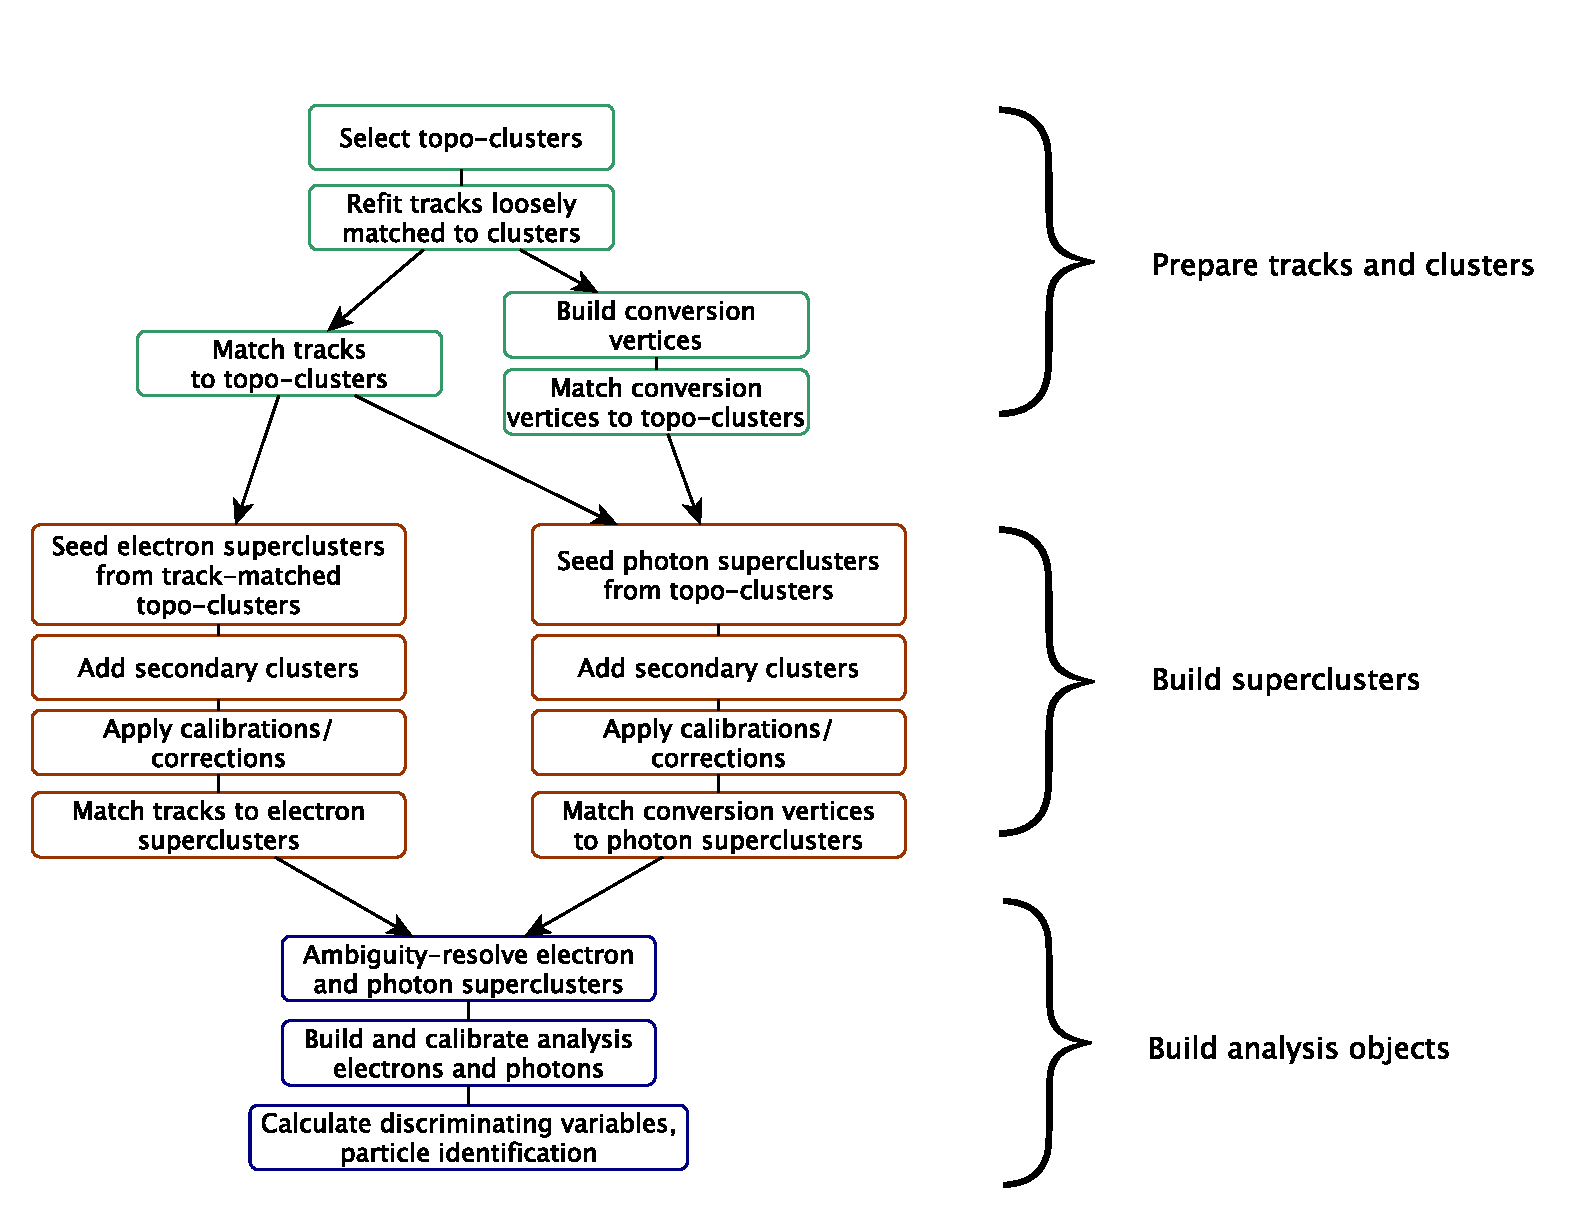
\includegraphics[width=0.8\linewidth]{3_experiment/object_reconstruction/egamma_reconstruction}
    \caption{Diagrama del algoritmo de reconstrucci\'on de electrones and fotones, extra\'ido de \Refn{\cite{ATLAS-EGamma-Performance-2015-2017}}}
    \label{fig:objects:egamma:reco:reco_diagram}
\end{figure}

El algoritmo para la reconstrucción de electrones y fotones procede como se muestra en la \Fig{\ref{fig:objects:egamma:reco:reco_diagram}}.
El proceso de reconstrucción comienza con la formación de \topos. Primero, se forman proto-clusters en el \ac{ECAL} y \ac{HCAL} agrupando celdas que tienen una energ\'ia requerida y predefinida, y añadiendo posteriormente celdas vecinas, obteniendo as\'i los \topos. Las reconstrucciones contin\'uan sólo en aquellos casos en los que la energía de los \topos en el \ac{ECAL} es superior a \(400~\mev\) y la fracci\'on de la misma con respecto a la energ\'ia total del \topo es mayor a \(0.5\), reduciendo gran parte los efectos de pileup.

El algoritmo también construye vértices de conversión a partir de las trazas reajustadas y los empareja con los \topos seleccionados.
Tras el ajuste inicial de las trazas y la construcción de las conversiones, los algoritmos de superclusters de electrones y fotones se ejecutan por separado y en paralelo. En la primera etapa, los \topos se evalúan para su uso como candidatos a clusters semilla, que forman la base de los superclusters; en la segunda etapa, los clusters cercanos a los candidatos a clusters semilla se identifican como candidatos a clusters satélite, que pueden surgir de la radiación bremsstrahlung o de la división de los \topos. Los clusters satélite que superan ciertos criterios de selecci\'on, se añaden a los candidatos a semilla para formar los superclusters finales.
Finalmente el algoritmo de reconstrucción hace coincidir las trazas con los superclusters de electrones y los vértices de conversión a los superclusters de fotones.

Dado que un objeto puede reconstruirse como electrón y como fotón, se resuelve esta ambigüedad para eliminar parte del solapamiento. Sin embargo, se permite cierto solapamiento para mantener una alta eficiencia de reconstrucción de electrones y fotones, y para que en cada an\'alisis de datos se apliquen criterios espec\'ificos a dicho estudio. Finalmente, se construyen y calibran los electrones y fotones finales.



\subsection{Identificaci\'on}
\label{subsec:objects:egamma:id}

Con el objetivo de poder discriminar los objetos \textit{prompt}\footnote{El término \textit{prompt} hace referencia a aquellos objetos producidos rápidamente luego de la colisión, generalmente provenientes del vértice primario, para distinguirlos de aquellos producidos por el decaimiento tardío de otra partícula, como puede ser un hadrón.} de aquellos que no lo son, existen diferentes criterios de identificaci\'on.
En \ac{ATLAS}, la identificaci\'on de fotones y electrones se logra mediante una serie de variables denominadas \acfp{SS} (descriptas en detalle en \Ch{\ref{ch:pid_ss}}). Estas, son variables que describen el paso de los fotones y electrones a trav\'es del \ac{ECAL} y \ac{HCAL}, caracterizando las lluvias electromagnéticas laterales y longitudinales, y son calculadas a partir de la energ\'ia depositada en las celdas de estos calor\'imetros. Mediante ciertos algoritmos que hacen uso de las \acp{SS}, se logra incrementar la pureza de los objetos deseados, al costo de tener una menor eficiencia de selecci\'on.
Finalmente, se definen diferentes \acp{WP} que son derivados de forma central y luego distribu\'idos a toda la colaboraci\'on.

El objetivo principal de la identificaci\'on de electrones es separar los electrones prompt de los electrones producto del proceso de creaci\'on de pares a partir de los fotones, de los jets que depositan energ\'ia en el \ac{ECAL}, y de los electrones proveninentes del decaimiento de hadrones originados por quarks de sabores pesados (\textit{heavy-flavor}). La identificaci\'on se basa en un m\'etodo likelihood que utiliza algunas de las \acp{SS}, utilizando electrones provenientes de decaimientos de \jpsi y \Zboson para bajo y alto \et, respectivamente~\cite{ATLAS-EGamma-Performance-2024}. Se definen entonces \acp{WP}, denominados \texttt{Loose}, \texttt{Medium} y \texttt{Tight}, cuyas eficiencias de identificaci\'on de un electr\'on con \(\et=40~\gev\) son de \(93\%, \, 88\%\) y \(80\%\), respectivamente~\cite{ATLAS-EGamma-Calibration-2015-2016}.


Para distinguir los fotones prompt/reales (los procedentes de la colisión) de los fotones de fondo que tienen secciones transversales de producción mucho mayores (procedentes del decaimiento de hadrones, también llamados fotones falsos), es necesario basarse en un algoritmo de identificación con alta eficiencia de señal y rechazo de fondo, para fotones candidatos con \(\pt \sim 10~\gev\) hasta la escala \tev.
Actualmente, la identificación de fotones en \ac{ATLAS} se basa en un conjunto de cortes rectangulares en las \acp{SS} mencionadas anteriormente.
El proceso completo de identificación de fotones se presenta en \Ch{\ref{ch:pid_ss}}, donde las \acp{SS} se explican una a una. Además, en el \Ch{\ref{ch:ffs}} se presentan dos enfoques para corregir las diferencias observadas en estas variables entre los datos y \ac{MC}, uno de los principales objetivos de esta tesis.





\subsection{Aislamiento}
\label{subsec:objects:egamma:iso}

Para mejorar aún más la selecci\'on de fotones y electrones se aplican criterios de aislamiento a estos objetos. Para ello, se definen dos criterios de aislamiento: calorim\'etrico y de trazas. 

\begin{figure}[ht!]
    \centering
    \includegraphics[width=0.5\linewidth]{3_experiment/object_reconstruction/isolation_diagram}
    \caption{Diagrama del proceso del c\'alculo de la variable de aislamiento calorim\'etrico. Cuando se utiliza un cono con \(R=0.4\), se puede construir la variable \etconefo mencionada en el texto.}
    \label{fig:objects:egamma:iso:iso_diagram}
\end{figure}

El procedimiento para calcular la energía de aislamiento calorim\'etrico \etconefo se esquematiza en la \Fig{\ref{fig:objects:egamma:iso:iso_diagram}}. En primer lugar, se construye un cono de radio \(\DeltaR<0.4\) alrededor del candidato a fotón o electrón, y se suman las energías de todas las celdas de los \topos (introducidos en la \Sect{\ref{subsec:objects:egamma:reco}}) cuyos baricentros se encuentran dentro del cono. A continuación, a esta energía calculada, se le resta la energía de todas las celdas en una ventana de \(5\times 7\) (en unidades de \(\eta \times \phi\) en la segunda capa del \ac{ECAL}) centrada alrededor del candidato, con el fin de eliminar la energía del propio candidato.
Tambi\'en se realizan correcciones para tener en cuenta las fugas de energ\'ia fuera del cono y las contribuciones de pileup~\cite{PileupSubstraction}. La forma final de la energ\'ia de aislamiento calorim\'etrico resulta:
\begin{equation*}
    \etconefo  = E_{T,\text{raw}}^{\text{isol}40} - E_{T,\text{core}} - E_{T,\text{leakage}} - E_{T,\text{pileup}}
\end{equation*}


La variable de aislamiento de trazas, \ptconetw, se obtiene sumando los \pt de las trazas de buena calidad en un cono de radio \(\DeltaR<0.2\) alrededor del candidato a electrón o en la dirección del cluster de fotones convertidos.
Se excluyen de este cómputo las trazas asociadas a la traza o al fotón convertido, así como aquellas trazas que no pasan el requisito de trazas de buena calidad. Una traza de buena calidad se define como aquella en la que el \(\pt>1~\gev\), y tiene una distancia mínima al vértice primario a lo largo del eje \(z\) de \(|z_0 \sin \theta| < 3\) mm.

En general, para los fotones y electrones, no hay otra energía depositada en el cono alrededor del candidato, aparte de los objetos de baja energía originados por los restos de la colisión, las interacciones múltiples y el pileup. En cambio, para los falsos candidatos a fotones y los fotones no directos, se observa energía adicional dentro del cono, originada por los objetos que acompañan al jet.

\begin{table}[ht!]
    \caption{Resumen de los \ac{WP} de aislamiento para electrones y fotones usados a lo largo de esta tesis.}
    \resizebox{\linewidth}{!}{
        \begin{tabular}{|l|c|c|c|}
            \hline
            Objecto                      & \ac{WP}                             & Aislamiento Calorim\'etrico                                    & Aislamiento de trazas   \\ \hline
            \multirow{3}{*}{Fot\'on}     & \texttt{FixedCutLoose}         & \(E_{T}^{\text{cone20}}<0.065\times \pt \)                & -                                  \\
                                        & \texttt{FixedCutTightCaloOnly} & \(\etconefo < 0.022\times \pt + 2.45~\gev\)               & -                                  \\
                                        & \texttt{FixedCutTight}         & \(\etconefo < 0.022\times \pt + 2.45~\gev\)               & \(\ptconetw/\pt < 0.05\)           \\ \hline
            \multirow{2}{*}{Electr\'on}   & \texttt{Loose\_VarRad}         & \(\etconetw < 0.2\times\pt\)                              & \(\pt^{\text{cone30}}/\pt < 0.15\) \\
                                        & \texttt{HighPtCaloOnly}        & \(\etconetw < \max\left(0.015\times\pt, 3.5~\gev\right)\) & -                                  \\ \hline
        \end{tabular}
    }
    \label{fig:objects:egamma:iso:iso_table}
\end{table}

A partir del aislamiento calorimétrico y de trazas se pueden definir diferentes \acp{WP} por separado tanto para electrones como para fotones. En el caso de los electrones, se definen dos estrategias: o bien conseguir una eficiencia fija, o bien aplicar cortes fijos en las variables de aislamiento. En el caso de los fotones, hay \acp{WP} que no utilizan ambas variables de aislamiento, como es el caso del \ac{WP} que sólo utiliza el aislamiento calorimétrico. Las definiciones de los diferentes \acp{WP} utilizados a lo largo de esta tesis se muestran en la \Tab{\ref{fig:objects:egamma:iso:iso_table}}. Además, es común definir las siguientes variables para \ac{WP} \texttt{FixedCutTight} del fotón:
\begin{align}
    \etiso &= \etconefo - 0.022 \times \et - 2.45~\gev\\
    \ptiso &= \ptconetw / \et
\end{align}
lo que resulta para el \ac{WP} \texttt{FixedCutTight} en:
\begin{align}
    \etiso &< 0 ~\gev\\
    \ptiso &< 0.05.
\end{align}















\section{Muones}



La tasa de radiación bremsstrahlung es inversamente proporcional al cuadrado de la masa de una partícula. Dado que los muones son unas 200 veces más pesados que los electrones, interactúan principalmente con el material del detector a través de ionización. Por lo tanto, los muones son partículas mínimamente ionizantes que no crean lluvia electromagnética en los calorímetros y atraviesan todas las capas del detector \ac{ATLAS}. Es por esta raz\'on que la detección de muones depende de las mediciones de las trazas dejadas por ellos en el \ac{ID} y el \ac{MS}. La combinación de los dos subdetectores define cuatro tipos de muones, dependiendo de la información utilizada para la reconstrucción:
\begin{itemize}
    \item \ac{CB}: mu\'on reconstruido a partir de un reajuste global de las trazas del \ac{ID} y del \ac{MS},
    \item \ac{ST}: mu\'on reconstruido a partir de una traza ajustada del \ac{ID} que al extrpolarla al \ac{MS} tienen un segmento en el \ac{MDT} o el \ac{CSC},
    \item \ac{CT}: mu\'on reconstruidos a partir de la traza del \ac{ID} ajustada a los depósitos de mínima energía ionizante en los calorímetros,
    \item \ac{ME}: mu\'on reconstruido únicamente a partir de las trazas \ac{MS}.
\end{itemize}

El solapamiento entre distintos tipos de muones se resuelve del siguiente modo. Cuando dos tipos de muones comparten la misma traza del \ac{ID}, el orden de preferencia es: primero el \ac{CB}, luego el \ac{ST} y finalmente el \ac{CT}. El solapamiento con \ac{ME} se resuelve analizando los hits de las trazas, seleccionando aquellas trazas con mejor ajuste y mayor número de hits.

Para la identificación de muones, se aplican cortes de calidad para distinguir los muones aislados de los procedentes de procesos de fondo, principalmente del decaimiento de piones y kaones.
Las variables con buen poder discriminatorio utilizadas se describen en \Refn{\cite{ATLAS-Muon-Performance-2016}}. Se definen cuatro selecciones de identificación: \texttt{Loose}, \texttt{Medium}, \texttt{Tight} y \texttt{High-pT}. Las tres primeras categorías son inclusivas, siendo \texttt{Medium} la selección por defecto en \ac{ATLAS}. Por último, se pide a los candidatos a muones que van a ser utilizados por los análisis que satisfagan los requisitos de aislamiento, tanto a nivel de trazas como calorimétricos, de forma análoga a los detallados para los electrones y fotones en el apartado anterior. Para el aislamiento de trazas, se utiliza una variable similar a la empleada para los electrones fotones, pero con un cono de radio variable \(\DeltaR = \min(10~\gev/\pt, 0.3)\) alrededor del momento del muón, excluyendo la traza del mismo. Para el aislamiento calorimétrico se utiliza la misma variable \etconefo, con la diferencia de utilizar un radio de \(R=0.2\), en lugar de \(0.4\). En base a estas variables, se definen 7 criterios de selección de aislamiento (7 \acp{WP}), optimizados para diferentes análisis.








\section{Jets}

Los quarks y gluones no pueden detectarse de manera aislada, sino que por un proceso denominado hadronizaci\'n, una vez producidos dan lugar a un chorro colimado de part\'iculas que se denomina \textit{jet}. Estos penetran a través del \ac{ECAL} y son totalmente absorbidos por el material del calorímetro hadrónico. A continuación, se describem los m\'etodos de reconstrucci\'on de jets utilizados en \ac{ATLAS}

\subsection{Algoritmo de clusterizaci\'on de jets \antikt}

Dado que los jets están constituidos por un elevado número de partículas que dejan deposiciones de energía en el \ac{ECAL} y \ac{HCAL} y trazas en el \ac{ID}, un algoritmo de clusterizaci\'on agrupa los constituyentes en el evento para definir los jets. Dicho algoritmo se denomina algoritmo \antikt~\cite{AntiKtAlgorithm}. Del mismo modo que para los electrones y los fotones, la reconstrucción de los jets en \ac{ATLAS} comienza en la formación de \topos: depósitos de energía agrupados en las celdas de los calorímetros mediante un algoritmo de combinación secuencial. Entonces, el algoritmo \antikt combina los \topos con los siguientes pasos:
\begin{itemize}
    \item Determinaci\'on de la distancia entre todos los \topos entre sí, y de cada \topo con el haz:
        \begin{gather}
            \dij = \min \left( p_{T,i}^{-2}, p_{T,j}^{-2} \right) \frac{\Delta_{i,j}^2}{R^2}\\
            d_{iB} = p_{T,i}^{-2}
        \end{gather}
        donde \(\Delta_{ij}^2 = \Delta\phi_{ij}^2 + \Delta\eta_{ij}^2\) y \(R\) es un valor fijo del algoritmo, que define el radio jet.
    \item Si el mínimo de todas las distancias calculadas anteriormente es \(d_{iB}\), el \topo \(i\) se clasifica como jet, y se descarta en iteraciones sucesivas.
    \item Si \(d_{ij} < d_{iB}\) se combinan los \topos \(i\) y \(j\), todas las distancias se calculan nuevamente con este nuevo \topo y la iteración se realiza de nuevo.
\end{itemize}
Este proceso se repite hasta que todas las partículas del evento se han agrupado.

El algoritmo \antikt tiende a unificar las part\'iculas \textit{soft} con las \textit{hard} y a separar a las part\'iculas \texttt{hard} entr s\'i, ya que la partícula con mayor \pt definirá el término \(\min \left( \frac{1}{p_{T,i}^2}, \frac{1}{p_{T,j}^2}  \right)\) en la definición de \dij. Esto permite que los jets del evento tengan una dirección estable al principio del proceso de combinación. El algoritmo \antikt es preferible a otros algoritmos secuenciales de jets ya que los jets tienen formas regulares que son aproximadamente cónicas, mostrados en la \Fig{\ref{fig:objects:jets:antikt}}. Los jets que se originan a partir de quarks o gluones en general se denominan small-\(R\) jets y para su reconstrucción se utiliza un radio de \(R=0.4\). Por otro lado, los jets que representan partículas masivas que decaen hadrónicamente se denominan large-\(R\) jets, y se utiliza \(R=1.0\), dado que el uso de un cono más amplio ayuda a incluir la mayoría de las partículas producto del decaimiento.


\begin{figure}[ht!]
    \centering
    \includegraphics[width=0.7\linewidth]{3_experiment/object_reconstruction/antikt_clusters}
    \caption{Representaci\'on esquem\'atica del algoritmo \antikt para el proceso de clusterizaci\'on de jets~\cite{AntiKtAlgorithm}.}
    \label{fig:objects:jets:antikt}
\end{figure}

\subsection{Jets Calorim\'etricos}

Una forma de reconstruir los jets se basa en los depósitos de energía en el calorímetro. De forma similar a lo que se ha explicado para electrones y fotones en la \Sect{\ref{subsec:objects:egamma:reco}}, los depósitos de energía en las celdas del \ac{ECAL} y \ac{HCAL} se utilizan para construir \topos, que se aproximan los depósitos de energía de hadrones individuales~\cite{ATLAS-TopoClusters-Run1,ATLAS-TopoClusters-Run2}. Los jets reconstruidos de esta manera y agrupados con el algoritmo \antikt con un radio de \(R=0.4\) se denominan jets \textsc{EMTopo}. En la reconstrucción de jets, sólo se incluyen los \topos con energía neta positiva.

\subsection{\acf{PFlow} Jets}

Otro m\'etodo para la reconstrucci\'on de jets se basa en el algoritmo \ac{PFlow}~\cite{ATLAS-JetPFlow-Performance}, en el que las mediciones del \ac{ID} y del calorímetro se combinan para formar las señales, que idealmente representan partículas individuales. El algoritmo comienza vinculando cada traza del \ac{ID} con un solo \topo y calcula la energ\'ia esperada en el calor\'imetro depositada por cada part\'icula que tambi\'en inici\'o la traza. Luego, para cada sistema \topo/traza, el algoritmo eval\'ua la probabilidad de que la energ\'ia de la part\'icula haya sido depositada en m\'as de un \topo, y decide si es necesario agregar m\'as \topos al sistema \topo/traza para recuperar la energ\'ia total del la lluvia. Posteriormente, la energ\'ia depositada por la part\'icula que inicia la traza es sustra\'ida celda por celda del conjunto de \topos vinculados. Finalmente, si la energ\'ia remanente en el sistema es consitente con la esperada por las fluctuaciones de la lluvia de la se\~nal de una sola part\'icula, los remanentes del \topo son removidos.

El resultado de este algoritmo es un conjunto de trazas, el conjunto de \topos, y un otro conjunto de \topos modificados por el procedimiento anterior. La combinaci\'on de estos 3 conjuntos definen un objecto \ac{PFlow}. Estos objetos también pueden ser agrupados con el algoritmo \antikt y con \(R=0.4\) para formar los jets \ac{PFlow}.

El algoritmo \ac{PFlow} tiene bastantes ventajas sobre el \textsc{EMTopo}:
\begin{itemize}
    \item La resolución en \pt del \ac{ID} es significativamente mejor que la resolución de energía del calorímetro para partículas cargadas de baja energía.
    \item Permite una mayor aceptancia para partículas más \textit{soft}. Las trazas se reconstruyen para partículas cargadas con un mínimo \pt de \(400~\mev\), el cual es menor que el requerido para la formaci\'on de \topos.
    \item Mejora la resolución angular de una sola partícula cargada, ya que utiliza la información del \ac{ID} en lugar de la del calorímetro.
    \item Las partículas cargadas de bajo \pt que se originan dentro de un jet hadrónico son barridas fuera del cono del jet por el campo magnético para cuando alcanzan el calorímetro. Utilizando la coordenada azimutal de las trazas en el perigeo, estas partículas tambi\'en son agrupadas en el jet.
    \item Es posible eliminar las trazas originadas por el pileup, sabiendo que éstas no proceden del \ac{PV}.
\end{itemize}

Cabe mencionarse, sin embargo, que para cualquier partícula cuya traza deba utilizarse, es necesario identificar correctamente y sustraer su señal en el calorímetro para evitar un doble conteo. En el algoritmo \ac{PFlow} se toma una decisión booleana sobre si utilizar la medición del \ac{ID} o del calorímetro. La capacidad de sustraer con precisión toda la energía de una sola partícula, sin eliminar la energía depositada por otras partículas, constituye el criterio clave de rendimiento sobre el que se optimiza el algoritmo.

En esta tesis, se consideran los jets \ac{PFlow}, ya que han demostrado proporcionar una mejor reconstrucción del jet~\cite{ATLAS-JetPFlow-Performance}.


\subsection{Calibraci\'on de jets}

Una vez reconstruidos los jets, su cuadrimomento se corrige para que coincida con la cinemática de un \textit{truth}-jet\footnote{Los truth jets, o jets reales, son jets asociados a una part\'icula espec\'ifica (jet iniciado por un quark de sabor liviano, por ejemplo) proveniente del estado final de una simulaci\'on, luego de pasar por el algoritmo de clusterizaci\'on \antikt.}. Las tres primeras correcciones tienen en cuenta la contaminación de la distribución de pileup subyacente y las fluctuaciones debidas al origen del jet~\cite{ATLAS-Jet-Calibration-Run2}. La \textit{Global Sequential Calibration} mejora la resolución de \pt de los jets (y las incertidumbres asociadas) eliminando secuencialmente la dependencia de la respuesta reconstruida del jet (\(R= E^{\text{reco}} / E^{\text{truth}}\)) en diversos observables. Por último, las diferencias residuales entre los datos y \ac{MC} se tienen en cuenta midiendo el desequilibrio de momento en \Zjets, \gammajet y eventos multijet.

Para reducir el número de jets con una fracción considerable de energía procedente del pileup, se utiliza el algoritmo \ac{JVT}. Este algoritmo \fixme{update to NNJVT} reconstruye un discriminante multivariante que combina, entre otras cantidades, el \ac{JVF} (fracción de las trazas \pt asociada a un jet originado por el \ac{PV}, y el número total de trazas) y el número de \acp{PV} en el evento \Npv. Como los jets que no proceden de la interacción hard-scatter son generalmente más suaves, el corte \ac{JVT} se aplica sólo a los jets con \(\pt<60~\gev\) y \(\abseta<2.4\). El \ac{JVT} \ac{WP} por defecto es \(96\%\) eficiente para los jets de dispersión dura.


















\section{Jets de sabor pesado (\textit{heavy flavor})}

Los decaimientos de hadrones pesados (de ahora en m\'as heavy-flavor) se rigen principalmente por el hadrón más pesado en la cascada de decaimiento. Un hadrón \(b\) generalmente decae en cascada a un hadrón \(c\), que a su vez decae a un hadrón \(s\), etc., lo que conduce a la existencia de múltiples vértices.

\ac{FTAG} es la clasificación de los jets dependiendo del sabor (\textit{flavor}) de los quarks por los que fueron iniciados, utilizando algoritmos sensibles a las propiedades distintivas de las respectivas clases. Entre ellos se consideran jets iniciados quarks \(b\) (\bjets), \(c\) (\cjets) o ni \(b\) ni \(c\) (jets livianos, tambi\'en referidos como light-jets o \ljets).
Estos complejos algoritmos se basan en los múltiples vértices, en la elevada masa, la alta multiplicidad de decaimientos y los modos de decaimiento característicos de los hadrones \(b\) y \(c\), así como en las propiedades de la fragmentación de los quarks pesados.


En \ac{ATLAS} se emplea un proceso de dos etapas para reconstruir las características clave de los heavy-flavor jets. En la primera etapa, los algoritmos de bajo nivel utilizan métodos complementarios para extraer información sobre las trazas de las partículas cargadas vinculadas al jet. Algunos algoritmos se centran en las propiedades de las trazas individuales, mientras que otros analizan sus correlaciones o las combinan para reconstruir explícitamente los vértices desplazados. En la segunda etapa, las salidas de estos algoritmos se integran en un algoritmo de alto nivel que utiliza clasificadores multivariantes para optimizar el rendimiento. Con el tiempo, los algoritmos han evolucionado significativamente, empezando con discriminantes basados en likelihoods y \acp{BDT} durante el Run-1 del \ac{LHC}, y avanzando hacia métodos más avanzados como las redes neuronales recurrentes y profundas, lo que ha dado lugar a notables mejoras en el rendimiento de la identificación~\cite{ATLAS-FTAG-Calibration-2012,ATLAS-FTAG-Efficiency-2012,MV2Algorithm,ATLAS-FTAG-DeepLearning}.

A partir del Run-3, el grupo de \ac{ATLAS} \ac{FTAG}, desarrolla un novedoso algoritmo "GN2" basado en un \textit{Transformer}. El algoritmo GN2 es un único modelo entrenado que sustituye a DL1d~\cite{ATLAS-FTAG-DL1-Run2} y a los algoritmos de bajo nivel que lo alimentan. Se basa en GN1~\cite{ATLAS-FTAG-GN1}, que se refinó para pasar a ser GN2. GN2 sustituye la \textit{Graph Attention Network}~\cite{GANs} utilizada por GN1 por un Transformador~\cite{GN2Transformer}, y también se beneficia de otras optimizaciones de arquitectura y de poder realizar el entrenamiento de la red con un orden de magnitud más de datos para su entrenamiento.

El algoritmo cepta directamente información sobre el jet y las trazas asociadas y, como tal, no depende de otros algoritmos de etiquetado de sabores (\textit{flavor tagging}). Mantiene los dos objetivos de entrenamiento auxiliares que se introdujeron con GN1: la agrupación de trazas que se originan en un vértice común y la predicción del proceso físico subyacente del que se originó cada traza.

Este nuevo algoritmo también está preparado para proporcionar la identificación de \cjets y jets procedentes de decaimientos \(\tau\). Las salidas de este tagger corresponden a las probabilidades de que un jet sea etiquetado (\textit{taggeado}) como un jet \(b\), \(c\), \(\tau\) o \textit{light}, denominadas como \(p_b\), \(p_c\), \(p_{\tau}\) y \(p_u\), respectivamente.

\subsection{Identificaci\'on y performance de \btagging}

Para evaluar la capacidad del tagger de identificar \bjets con una eficiencia constante, se mide la capacidad de rechazar los jets \(c\), \(\tau\) y light. Las probabilidades de salida del tagger se combinan para construir un único discriminante \gntb, definido como
\begin{equation}
    \gntb = \log \left(
        \frac{p_b}{f_c p_c + f_{\tau} p_{\tau} + \left(1-f_c-f_{\tau}p_u\right)}
    \right).
\end{equation}
Los parámetros \(f_{c(\tau)}\) son libres y determinan la importancia entre \(p_{c(\tau)}\) y \(p_u\) en el discriminante. Los valores específicos de estos parámetros se determinan mediante un procedimiento de optimización maximizando el rechazo de \cjets (\(\tau\)-jets) y \ljets, y resultan ser \(0.2\) (\(0.01\)).


A partir del valor discriminante del tagger, se pueden definir varios \acp{WP}, simplemente exigiendo que el valor \gntb esté por encima de un determinado umbral. El grupo \ac{FTAG} de \ac{ATLAS} proporciona de forma centralizada a toda la colaboración cinco \acp{WP} diferentes para lograr una eficiencia global fija de \btagging: \(65,\, 70,\, 77,\, 85\) y \(90\%\), y se muestran en la \Fig{\ref{fig:objects:jet_tagging:btag_discrminant}}. En dicha figura se comparan tambi\'en las distribuciones de datos y \ac{MC} del tagger GN2, donde las contribuciones de los distintos sabores se muestran con colores diferentes.

\begin{figure}[ht!]
    \centering
    \includegraphics[width=0.6\linewidth]{3_experiment/object_reconstruction/btagging_discriminant}
    \caption{Comparaci\'on entre datos y simulaci\'on \ac{MC} (eventos del proceso \ttbar semilept\'onico) del discriminante del tagger GN2. Las contribuciones de los jets \(l\), \(b\) y \(c\) se muestran con diferentes colores, y los 5 \acp{WP} de \btagging se muestran con las l\'ineas verticales punteadas. De izquierda a derecha, las l\'ineas representan los \acp{WP} de \(90, 85, 77, 70\) y \(65\%\) de eficiencia. El panel inferior muestra el ratio entre los datos y la suma de las simulaciones \ac{MC}~\cite{ATLAS-FTAG-GN2BtagWPs}.}
    \label{fig:objects:jet_tagging:btag_discrminant}
\end{figure}

Uno de los principales problemas del \btagging es la disminución de la eficiencia a mayor \pt. En este régimen de \pt elevado, las partículas est\'an m\'as colimadas y tienden a viajar más lejos en el \ac{ID} antes de decaer, lo que puede dar lugar a una traza de decaimiento con hits espurios. La degradación de la eficiencia se visualiza en la \Tab{\ref{tab:objects:ftag:btag_efficiency_original}}, donde se muestran las eficiencias de tagging para \bjets, junto con los rechazos a \cjets, \ljets y \tjets, en los regímenes de bajo y alto \pt. Los valores mostrados se calculan utilizando diferentes muestras, en las que \ttbar se utiliza en la región bajo de \pt y eventos de decaimiento de \(Z'\)~\footnote{El modelo leptof\'obico de vector axial \(Z'\) es un modelo de Materia Oscura simplificado en el cual el decaimiento teorizado es un par de quarks.} se utilizan en la región alto de \pt. Puede verse que la eficiencia de \btag cae en un \(30\%\) para jets de \pt más alto.

\begin{table}[ht!]
    \caption{Medidas de eficiencias de \btagging, y de rechazos de \cjets, \ljets y \tjets, en los regímenes de bajo y alto \pt.}
    \label{tab:objects:ftag:btag_efficiency_original}
    \resizebox{\textwidth}{!}{
        \begin{tabular}{llcccc}
            \toprule
            Muestra & Rango de \pt [\gev]                                    & Eficiencia de \bjet & Rechazo de \cjet & Rechazo de \ljet & Rechazo de \tjet \\ \midrule
            $t\bar{t}$  & \(20<\pt<250\)    & $0.76$         & $17.52$       & $448.61$               & $71.15$          \\
            $Z'$        & \(250<\pt<6000\)  & $0.41$         & $20.27$       & $179.99$               & $452.94$         \\ \bottomrule
        \end{tabular}
    }
\end{table}

\subsection{Identificaci\'on y performance de \ctagging}

Al igual que con \btagging, se puede construir un único discriminante a partir de las probabilidades dadas por el tagger para identificar \cjets frente a \bjets, \tjets y \ljets:
\begin{equation}
    \gntc = \log \left(
        \frac{p_c}{f_b p_b + f_{\tau} p_{\tau} + \left(1-f_b-f_{\tau}p_u\right)}
    \right)
\end{equation}
donde ahora los valores \(f_{b(\tau)}\) son los parámetros libres que controlan el rechazo entre jets \(b\), \(\tau\) y light. Utilizando el mismo procedimiento de optimización que para \btagging, los valores para \(f_{b(\tau)}\) resultan ser \(0.3\) (\(0.05\)).

Gracias a la gran eficiencia \btagging conseguida por GN2, es posible diseñar un \ac{WP} de \ctagging tras aplicar un veto de \btagging, separando aún más los \cjets de los \ljets. Construyendo este \ac{WP} de tagging simultáneo y asumiendo que la fracción de \tjets es despreciable, se puede separar los jets \(b\), \(c\) y livianos en tres regiones ortogonales. Partiendo de exigir que un jet \textit{no} pase el \ac{WP} de \btagging de \(77\%\) de eficiencia (veto \btag), se definen tres \acp{WP} diferentes de \ctagging definidos para eficiencias de \(10, \, 30\) y \(50\%\), fijando el valor de \gntc. Las medidas de eficiencia y rechazo de las dos muestras descriptas anteriormente, tras aplicar el \ac{WP} de \ctag de \(50\%\) de eficiencia se muestran en el \Tab{\ref{tab:objects:ftag:ctag_efficiency_original}}.

\begin{table}[ht!]
    \caption{Medidas de eficiencia de \ctagging para \cjets, y valores de rechazos de \bjets, \ljets y \tjets en los regímenes de bajo y alto \pt. Los valores corresponden a aquellos luego de aplicar el veto del \ac{WP} de \btagging de \(77\%\) y de \(50\%\)  de \ctagging. \fixme{rejection values not correct!}}
    \label{tab:objects:ftag:ctag_efficiency_original}
    \resizebox{\linewidth}{!}{
        \begin{tabular}{llcccc}
            \toprule
            Muestra & Rango de \pt [\gev]   & Eficiencia de \cjet & Rechazo de \bjet & Rechazo de \ljet & Rechazo de \tjet \\ \midrule
            $t\bar{t}$  & \(20<\pt<250\)    & $0.467$         & $17.52$       & $448.61$               & $71.15$          \\
            $Z'$        & \(250<\pt<6000\)  & $0.344$         & $20.27$       & $179.99$               & $452.94$         \\ \bottomrule
        \end{tabular}
    }
\end{table}


\FloatBarrier
\part{Correcciones de las Shower shapes de fotones}
\label{part:pid}
\chapter{Shower shapes y la Identificaci\'on de fotones}
\label{ch:pid_ss}
% \epigraph{\emph{“Champions keep playing until they get it right.”}}{Billie Jean King}



El \ac{ECAL} se presentó brevemente en la \Sect{\ref{subsubsec:atlas:atlas:cals:ecal}}, donde se describió el mecanismo que se utiliza para la medida de energ\'ia y posici\'on de fotones y electrones. En este subdetector, los fotones depositan su energía mediante la creación de pares electrón-positrón y la radiación bremsstrahlung, creando una lluvia \acf{EM}. El \ac{ECAL} es eficiente para calcular la energía de la lluvia \ac{EM}, pero identificar la partícula iniciadora sigue siendo una tarea difícil.
Sin embargo, en virtud de las diferentes capas y granularidades en el \ac{ECAL}, pueden estudiarse diferentes características de estas lluvias \ac{EM}, codificadas por diferentes variables llamadas \acfp{SS}.

El cap\'itulo comienza con la descripci\'on de todas las \acp{SS}, que son centrales para poder identificar a los fotones reales de los falsos.
% Las variables mencionadas se utilizan mucho en el proceso de identificación de fotones, ya que proporcionan la separación necesaria entre fotones reales y falsos.
La optimizaci\'on del algoritmo de identificaci\'on de fotones utiliza las \acp{SS}, y se encuentra descripta en la \Sect{\ref{sec:pid_ss:pid}}. Adem\'as, en dicha secci\'on, se presentan los m\'etodos usados para la estimaci\'on de las eficiencias de identificaci\'on de fotones.
Por último, en la \Sect{\ref{sec:pid_ss:ss_differences}} se describe brevemente las deficiencias en el modelado de las \acp{SS} en las simulaciones, un problema que tiene implicancias directas en los c\'alculos de eficiencias. Este problema y sus posibles soluciones ser\'an estudiadas en detalle en el \Ch{\ref{ch:ss_corrections}}.






\section{Shower shapes}
\label{sec:pid_ss:ss}

Como se menciona en la \Sect{\ref{subsec:objects:egamma:id}}, la identificación de fotones se realiza aplicando cortes rectangulares a las diversas \acp{SS} que proveen una excelente capacidad de separación entre fotones reales aislados de fotones falsos procedentes de hadrones. Las \acp{SS} se calculan a partir de los depósitos de energía de los candidatos a fotones en las celdas del \ac{ECAL} y \ac{HCAL}, caracterizando la forma lateral y longitudinal de las lluvias \ac{EM}, y sirven para describir el paso de los fotones por los calorímetros.

En general, los fotones reales producen depósitos de energía más angostos en el \ac{ECAL}, y tienen menores filtraciones hacia el \ac{HCAL}, en comparación con aquellos fotones procedentes de hadrones, donde la presencia de hadrones vecinos adicionales cerca del fotón falso tienden a ensanchar las lluvias. Además, dado que la primera capa del \ac{ECAL} presenta una gran resoluci\'on en \(\eta\), es posible discriminar los candidatos a fotones procedentes de decaimientos \(\pizero\to\gamma\gamma\) que est\'an caracterizados por dos máximos locales debidos a la presencia de dos fotones cercanos.

\begin{table}[ht!]
    \caption{\acfp{SS} utilizadas para la identificaci\'on de fotones. Las tres columnas de la derecha denotan si la variable es utilizada o no para los \acp{WP} \texttt{Loose} (L), \texttt{Medium} (L) o \texttt{Tight} (T), descriptos en la \Sect{\ref{subsec:pid_ss:pid:optimisation}}.}
    \centering
    \resizebox{\textwidth}{!}{
        \begin{tabular}{p{.2\textwidth}p{.50\textwidth}p{0.12\textwidth}|p{.01\textwidth}p{.01\textwidth}p{.01\textwidth}}
            \hline
            \hline
            Categor\'ia  &  Descripci\'on  &  Nombre & L & M & T \\
            \hline
            \hline
            Filtraci\'on hadr\'onica
            &  Cociente entre el \et en la primera capa del \ac{HCAL} y el \et del cluster \ac{EM} (\(\abseta<0.8\) y \(\abseta>1.52\))
            &  \(R_{\text{had 1}}\)  & \checkmark & \checkmark & \checkmark\\
            &  Cociente entre el \et en todo el \ac{HCAL} y el \et del cluster \ac{EM} (\(0.8<\abseta<1.37\))
            &  \(R_{\text{had}}\) & \checkmark & \checkmark & \checkmark\\
            \hline
            \ac{ECAL} (\(2^{\text{da}}\) capa)
            &  Cociente entre la energ\'ia sumada en \(3\times 7\) celdas en \(\eta \times \phi\)  y la energ\'ia en \(7 \times 7\) celdas, centradas alrededor del centro del cluster
            &  \(R_{\eta}\) & \checkmark & \checkmark & \checkmark\\
            &  Ancho lateral de la lluvia en direcci\'on de \(\eta\) & \(w_{\eta 2}\)  & \checkmark & \checkmark & \checkmark\\
            &  Cociente de la energ\'ia sumada en \(3 \times 3\) celdas en \(\eta \times \phi\) y en \(3 \times 7\) celdas, centradas alrededor del centro del cluster
            &  \(R_{\phi}\) &  & \checkmark & \checkmark\\
            \hline
            \ac{ECAL} (\(1^{\text{ra}}\) capa)
            &  Ancho lateral de la lluvia en 3 \textit{strips} alrededor del m\'aximo
            &  \(w_{\eta 1}\) or \(w_1\) &  & \checkmark & \checkmark\\
            &  Ancho lateral total de la lluvia
            &  \(w_{\text{s tot}}\) &  & \checkmark & \checkmark\\
            &  Fracci\'on de la energ\'ia fuera de las 3 strips centrales en un rango de 7 celdas, sobre la energ\'ia en las 3 celdas centrales &  \(f_{\text{side}}\)  &  & \checkmark & \checkmark\\
            &  Diferencia entre la energ\'ia del segundo m\'aximo con la energ\'ia m\'inima entre los dos primeros m\'aximos.
            &  \(\Delta E\)  &  & \checkmark & \checkmark\\
            &  Cociente de la diferencia de energ\'ia entre el primer y segundo m\'aximo, sobre la suma de ambas energ\'ias
            &  \(E_{\text{ratio}}\)  &  & \checkmark & \checkmark\\
            &  Cociente de la energ\'ia en la primera capa del \ac{ECAL} y la energ\'ia total del cluster \ac{EM}
            &  \(f_1\) & & \checkmark & \checkmark\\
            \hline
            \hline
        \end{tabular}
    }
    \label{tab:pid_ss:ss:ss_variables}
\end{table}

\begin{figure}[ht!]
    \centering
    \includegraphics[width=\linewidth]{4_photonid/introduction/diagrams/shower-shapes}
    \caption{Representaci\'on esquem\'atica de las \ac{SS} de fotones.}
    \label{fig:pid_ss:ss:ss_variables}
\end{figure}

A continuación, se detallan las \acp{SS} utilizadas para la identificación de fotones, que se muestran resumidas en \Tab{\ref{tab:pid_ss:ss:ss_variables}} y un esquema de c\'omo son calculadas se encuentra en la \Fig{\ref{fig:pid_ss:ss:ss_variables}}.
Las primeras variables hacen uso de la energía medida en el \ac{HCAL}:
\begin{itemize}
    \item Filtraci\'on hadr\'onica: es la energía transversal depositada en el \ac{HCAL}, normalizada respecto a la energía depositada en el \ac{ECAL}:
        \begin{equation}
            {\rhad}_{(1)} = \frac{\et^{\text{HCAL}}}{\et^{\text{ECAL}}}
        \end{equation}
        Para minimizar los efectos de la degradación de la resolución, en la región de transición barrel-endcap del \ac{HCAL} (\(0.8\leq \abseta\leq 1.37\)) se utiliza la energía depositada en todo el \ac{HCAL} (\rhad). En el resto del detector, sólo se utiliza la energía depositada en la primera capa del \ac{HCAL} (\rhado).
\end{itemize}
Las siguientes variables utilizan la información de la segunda capa del \ac{ECAL}:
\begin{itemize}
    \item Perfil de energía lateral en \(\eta\):
        \begin{equation}
            \reta = \frac{E_{3\times7}^{s2}}{E_{7\times7}^{s2}}
        \end{equation}
        donde \(E_{i\times j}^{s2}\) es la suma de energía en la segunda capa del calorímetro contenida en una ventana de \(i \times j \) celdas (unidades de \(\eta \times \phi\)), centrada en la celda más energética. Esta variable da una medida del ancho de las lluvias en la dirección \(\eta\).
    \item Perfil de energía lateral en \(\phi\):
        \begin{equation}
            \rphi = \frac{E_{3\times3}^{s2}}{E_{3\times7}^{s2}}
        \end{equation}
        definida de forma similar a \reta. Sin embargo, esta variable se comporta de forma muy diferente para fotones convertidos y no convertidos. Debido a la acción del campo magnético, los electrones y positrones se curvan en direcciones opuestas en \(\phi\), por lo que se producen lluvias \ac{EM} más anchas para los fotones convertidos que para los no convertidos.
    \item Ancho de la lluvia lateral en \(\eta\):
        \begin{equation}
            \weta = \sqrt{
                \frac{\sum E_i \eta_i^2}{\sum E_i}
                -
                \left(\frac{\sum E_i \eta_i}{\sum E_i}\right)^2
            }
        \end{equation}
        mide el ancho propio de la lluvia \ac{EM}, donde \(E_i\) es la energía en la \(i\)-ésima celda del \ac{ECAL}, medida en una ventana de \(3\times 5 \) celdas en \(\eta \times \phi\).
\end{itemize}
Las siguientes variables utilizan la información de la primera capa del \ac{ECAL}, compuesta por las celdas \textit{strips} que permiten una alta resolución en \(\eta\) y permite una buena separación entre fotones aislados de fotones producto del decaimiento de \(\pizero\). La \Fig{\ref{fig:pid_ss:ss:pizero}} muestra la diferencia en la energía depositada en el \ac{ECAL} entre los dos casos mencionados anteriormente.
\begin{itemize}
    \item Perfil de energía lateral en \(\eta\):
        \begin{equation}
            \fside = \frac{E_7^{s1} - E_3^{s1}}{E_3^{s1}}
        \end{equation}
        mide la energía fuera del núcleo de las tres strips centrales dentro de una ventana de 7 celdas, dividida por la energía en las tres celdas centrales.
    \item Ancho de la lluvia lateral en \(\eta\) (3 strips)
        \begin{equation}
            \wone = \sqrt{
                \frac{\sum E_i (i - i_{max})^2}{\sum E_i}
            }
        \end{equation}
        donde \(i\) corre sobre todas las celdas en una ventana de 3 celdas alrededor de la de mayor energía. Esta variable mide el ancho de la lluvia \ac{EM} en la primera capa del calorímetro.
    \item Ancho de la lluvia lateral en \(\eta\) (total).
        Se define de forma similar a \wone, pero utiliza todas las celdas en una ventana de \(\Delta\eta\times\Delta\phi=0.0625\times 0.2\), que corresponde aproximadamente a \(20\times 2\) strips en \(\eta\times\phi\).
    \item Diferencia energética
        \begin{equation}
            \deltae = E_{\text{max}, 2}^{s1} - E_{\text{min}}^{s1}
        \end{equation}
        representa la diferencia de energía entre el segundo máximo y la energía mínima reconstruida entre los dos máximos de la primera capa del \ac{ECAL}.
    \item Asimetr\'ia de energía
        \begin{equation}
            \eratio = \frac{
                E_{\text{max}, 1}^{s1} - E_{\text{max}, 2}^{s1}
            }{
                E_{\text{max}, 1}^{s1} + E_{\text{max}, 2}^{s1}
            }
        \end{equation}
        es la relación de la diferencia de energía entre los dos máximos, normalizada con respecto a la suma de esas energías, en la primera capa del \ac{ECAL}.
\end{itemize}

\begin{figure}[ht!]
    \centering
    \includegraphics[width=0.7\linewidth]{4_photonid/introduction/diagrams/PhotonPizero}
    \caption{Dep\'ositos de energ\'ia caracter\'isticos para un fot\'on aislado (izquierda), y un evento \(\pizero\to\gamma\gamma\) (derecha), que es posible distinguir gracias a la fina granularidad de la primera capa del \ac{ECAL}~\cite{ATLAS-ECAL-Pizero}.}
    \label{fig:pid_ss:ss:pizero}
\end{figure}






\section{Identificaci\'on de fotones}
\label{sec:pid_ss:pid}

La identificación de fotones prompt frente a fotones falsos en colisiones hadrónicas es un gran desaf\'io. Los fotones falsos están ampliamente dominados por candidatos a fotones que surgen del decaimiento de hadrones en jets, mientras que una fracción más pequeña de candidatos falsos está asociada con hadrones que depositan una energía significativa en el \ac{ECAL}, imitando la de los fotones reales.
Los procesos con fotones prompt en el estado final, que ocurren en colisiones \pp en el \ac{LHC}, desempeñan un papel central en el programa de física de \ac{ATLAS}. Tanto para las búsquedas como para las medidas de precisión es importante contar con algoritmos y técnicas para identificar los fotones reales frente a los falsos. Estas b\'usquedas o medidas de precisi\'on se llevan a cabo en un rango muy amplio de energ\'ia del fotón, empezando, por ejemplo, por resonancias de baja masa del Higgs a un par de partículas tipo axión que decaen en 4 fotones (\(\PH\to aa \to 4\gamma\))~\cite{ATLAS-HiggsTo4Gamma}, donde el momento transverso del fotón es de \(\sim 25~\gev\), hasta fotones de muy alto \pt en búsquedas de resonancias \gammajet como los que se realizaron para esta tesis, donde los fotones tienen un momento transverso mayor a \(1~\tev\) (\Part{\ref{part:search}}).

La identificaci\'on de fotones en \ac{ATLAS} se basa en cortes en las \acp{SS} y se definen diferentes \acfp{WP} con diferentes caracter\'isticas: ya sea lograr un gran rechazo de fondo, o alta eficiencia de se\~nal, o simplemente bajos tiempos de c\'omputo para la identificaci\'on \textit{online}. En esta sección se describe el procedimiento utilizado para la optimizaci\'on de estos \acp{WP} y luego se describen los m\'etodos para medir las eficiencias correspondientes.



\subsection{Procesos de inter\'es y selecci\'on de eventos}
\label{subsec:pid_ss:pid:event_selection}

Dado el amplio rango de energ\'ias en el que se utilizan los fotones en \ac{ATLAS}, para la optimización de los \acp{WP} se utilizan dos procesos diferentes que permiten obtener muestras limpias de fotones en los regímenes de bajo y alto \pt. En el caso de bajo \pt, se utiliza una fuente muy limpia de fotones procedentes de decaimientos radiativos del bos\'on \Zboson. Por otro lado, aunque con mayor contaminación de fondo, se emplean eventos de fotones prompt (ver la \Sect{\ref{subsec:theory:sm:prompt_photon}}) para fotones de alto \pt. En los siguientes párrafos se ofrece una descripción de cada de las muestras de fotones utilizadas.


\paragraph{Decaimientos radiativos del bos\'on \Zboson}

En el rango de bajo \pt, se utilizan fotones procedentes del decaimiento radiativo del bosón \Zboson (\(\Zboson \to \ell\ell \gamma\)). Hay dos modos de producción posibles para los procesos del \ac{SM} de \(\pp\to \Zboson(\ellell)\gamma\), donde \(\ell\) es un electrón o un mu\'on. Estos son: \acf{ISR} donde el fotón es radiado por los quarks, y \acf{FSR}, donde el fotón es radiado por uno de los leptones del estado final a través de bremsstrahlung. Ambos modos de producción se muestran en la \Fig{\ref{fig:pid_ss:event_selection:fsr_isr}}.


\begin{figure}[ht!]
    \centering
    \begin{subfigure}[h]{0.49\linewidth}
        \centering
        \includegraphics[width=0.6\linewidth]{4_photonid/introduction/diagrams/isr}
        \caption{\acf{ISR}}
    \end{subfigure}
    \hfill
    \begin{subfigure}[h]{0.49\linewidth}
        \centering
        \includegraphics[width=0.6\linewidth]{4_photonid/introduction/diagrams/fsr}
        \caption{\acf{FSR}}
    \end{subfigure}
    \caption{Diagrams de Feynman del proceso de radiaci\'on de un fot\'on en decaimientos \(\Zboson\to\ell\ell\gamma\) para los casos de \ac{ISR} (izquierda) y \ac{FSR} (derecha).}
    \label{fig:pid_ss:event_selection:fsr_isr}
\end{figure}


Ambos procesos \ac{FSR} y \ac{ISR} pueden identificarse fácilmente comparando la distribución de la masa invariante de los dos leptones (\mll) con la distribución de la masa invariante de los dos leptones junto con el fot\'on (\mlly).
Para los eventos \ac{ISR}, \mll tiene su m\'aximo en el valor de la masa del \Zboson, y el fotón simplemente suma a la masa invariante de tres cuerpos (\mlly) haciéndola mayor que \(\sim 91~\gev\). En el caso \ac{FSR}, en cambio, la masa invariante de tres cuerpos \mlly presenta su m\'aximo en el valor de la masa del \Zboson.
% , observado en la \Fig{\ref{fig:pid_ss:event_selection:mll_mlly_distribution:data}}.
Para los estudios de identificación de fotones sólo se consideran los fotones de los eventos \ac{FSR} (de ahora en m\'as también referido como decaimiento \acf{RZ}). Los eventos \ac{ISR} también sufren la contaminación de fondos provenientes de eventos \Zjets, en los que el jet se identifica erróneamente como un fotón, y adem\'as la sección eficaz \Zjets es de varios \'ordenes de magnitud mayor a la del proceso \(\Zboson+\gamma\). A partir de las \Figs{\ref{fig:pid_ss:event_selection:mll_mlly_distribution:bkg}}{\ref{fig:pid_ss:event_selection:mll_mlly_distribution:signal}}, donde se muestran las distribuciones de \mll en funci\'on de \mlly para los procesos simulados de \(\Zboson\to\ell\ell\) y \(\Zboson\to\ell\ell\gamma\), respectivamente, se puede apreciar la separación entre estos dos procesos cuando se seleccionan fotones \ac{FSR}.

\begin{figure}[ht!]
    \centering
    \begin{subfigure}[h]{0.32\linewidth}
        \centering
        \includegraphics[width=\linewidth]{4_photonid/introduction/can2d__data__nosel__llg_m_ll_m__RZ__rel22_run2_Run2}
        \caption{Data}
        \label{fig:pid_ss:event_selection:mll_mlly_distribution:data}
    \end{subfigure}
    \hfill
    \begin{subfigure}[h]{0.32\linewidth}
        \centering
        \includegraphics[width=\linewidth]{4_photonid/introduction/can2d__bkg__nosel__llg_m_ll_m__RZ__rel22_run2_Run2}
        \caption{\(\Zboson\to \ell\ell\)}
        \label{fig:pid_ss:event_selection:mll_mlly_distribution:bkg}
    \end{subfigure}
    \hfill
    \begin{subfigure}[h]{0.32\linewidth}
        \centering
        \includegraphics[width=\linewidth]{4_photonid/introduction/can2d__signal__nosel__llg_m_ll_m__RZ__rel22_run2_Run2}
        \caption{\(\Zboson\to \ell\ell\gamma\)}
        \label{fig:pid_ss:event_selection:mll_mlly_distribution:signal}
    \end{subfigure}
    \caption{Masa invariante de los dos leptones en funci\'on de la masa invariante de ambos leptones junton con un fot\'on en (\subref{fig:pid_ss:event_selection:mll_mlly_distribution:data}) datos, (\subref{fig:pid_ss:event_selection:mll_mlly_distribution:bkg}) fondos y (\subref{fig:pid_ss:event_selection:mll_mlly_distribution:signal}) se\~nal. La reg\'on en la cual se encuentra una gran concentraci\'on de eventos con \(m_{\ell\ell} \sim m_{\Zboson}\) corresponde a eventos de \ac{ISR}, mientras que eventos de \ac{FSR} events est\'an caracterizados por \(m_{\ell\ell\gamma} \sim m_{\Zboson}\).}
    \label{fig:pid_ss:event_selection:mll_mlly_distribution}
\end{figure}

Se requiere que los fotones tengan un momento transverso \(\pt>7~\gev\) y una pseudorapidez en el rango de \(\abseta<1.37\) o \(1.52<\abseta<2.37\), evitando as\'i la región del crack.
Para los estudios de optimización no se aplica ningún requisito de aislamiento sobre los fotones, pero para las medidas de eficiencia se utiliza el \ac{WP} de aislamiento \texttt{Loose}, descripto en la \Sect{\ref{subsec:objects:egamma:iso}}. Se requiere que los leptones tengan \(\et>10~\gev\), los muones una pseudorapidez \(\abseta<2.5\) y para los electrones \(\abseta<2.47\), excluyendo el crack. Tanto a los electrones como a los muones se les exige que pasen los requisitos de aislamiento \texttt{Loose} y que pasen el criterio de identificación \texttt{Medium}.

El fotón \ac{FSR} se selecciona entonces requiriendo \(80<\mlly<100~\gev\) y \(40<\mll<83~\gev\). Finalmente, para evitar cualquier sesgo en las \ac{SS} del fotón y en sus variables de aislamiento, se requiere una distancia mínima de \(\DeltaR>0.4\) entre dicho fot\'on y el leptón más cercano.


\paragraph{\acf{SP}}

La muestra de fotones inclusivos, o \acf{SP}, se recoge mediante triggers que requieren un s\'olo fot\'on con umbrales que var\'ian entre \(10~\gev\) y \(140~\gev\) e identificación \texttt{Loose}. Aunque los triggers utilizados para obtener esta muestra están preescalados (con la excepción del de \(140~\gev\)), proporcionan un gran conjuntos de datos de fotones de alto \pt.
Estos procesos incluyen eventos a \ac{LO} de \gammajet procedentes de la dispersión dura \(qg\to q\gamma\) y \(\qqbar \to g\gamma\), así como fotones prompt procedentes de la fragmentación de quarks en eventos de dijet de \acs{QCD}.
Se requiere que estos fotones presenten una pseudorapidez de \(\abseta<2.37\) excluyendo el crack, y pasar el requisito de aislamiento \texttt{Loose}. Las muestras de \ac{SP} se utilizan tanto para los estudios de optimización como para la estimaci\'on de las eficiencias.


\subsection{Optimizaci\'on}
\label{subsec:pid_ss:pid:optimisation}

A partir de las \acp{SS} anteriormente descriptas se definen tres \acp{WP} para los fotones: \texttt{Loose}, \texttt{Medium} y \texttt{Tight}~\cite{ATLAS-EGamma-Performance-2024}. El \ac{WP} loose emplea cortes a las variables definidas en la segunda capa y a la variable de filtraci\'on hadrónica, y es utilizado principalmente por el trigger.
Los \acp{WP} medium y tight utilizan todas las variables definidas previamente. El \ac{WP} medium está optimizado para tener una eficiencia fija de \(95\%\), mientras que el \ac{WP} tight proporciona un excelente rechazo de fondo. La \Tab{\ref{tab:pid_ss:ss:ss_variables}} muestra qué variables se utilizan para cada \ac{WP}.

Para la optimización de los \acp{WP} se utilizan las dos muestras definidas previamente: los eventos \ac{RZ} para fotones con \(10<\pt<25~\gev\) como señales y eventos de \(\Zboson\to \ell\ell\) como fondos; y para el régimen de alto \pt (\(\pt>25~\gev\)) los eventos de \ac{SP} se consideran como señal mientras que los eventos dijet son los fondos.

En la \Fig{\ref{fig:pid_ss:optimisation:shower_shapes}} se muestran ejemplos de tres de estas \ac{SS} (\reta, \eratio y \weta) comparando eventos de señal y de fondo utilizando las muestras de \ac{RZ}, donde se observa un excelente poder discriminatorio.
Los cortes en todas las \acp{SS}, para cada \ac{WP} de identificación, se obtienen en función de la energía transversal y la pseudo-rapidez del candidato a fotón, para tener en cuenta la forma de las variables para diferentes \(\eta\) y para variaciones en la cantidad de material y la geometría del calorímetro. Los \acp{WP} medium y tight también se calculan por separado para fotones convertidos y no convertidos.
Los cortes se optimizan utilizando un enfoque multivariable, en el que las eficiencias de señal se escanean entre \(0\%\) y \(100\%\) mientras se intenta maximizar el rechazo de fondo.

\begin{figure}[ht!]
    \centering
    \begin{subfigure}[h]{0.32\linewidth}
        \centering
        \includegraphics[width=\linewidth]{4_photonid/introduction/shower_shapes/can__sigbkg__presel__ph_reta__RZ__rel22_run2_Run2}
        \caption{\reta}
        \label{fig:pid_ss:optimisation:shower_shapes:reta}
    \end{subfigure}
    \hfill
    \begin{subfigure}[h]{0.32\linewidth}
        \centering
        \includegraphics[width=\linewidth]{4_photonid/introduction/shower_shapes/can__sigbkg__presel__ph_eratio__RZ__rel22_run2_Run2}
        \caption{\eratio}
        \label{fig:pid_ss:optimisation:shower_shapes:eratio}
    \end{subfigure}
    \hfill
    \begin{subfigure}[h]{0.32\linewidth}
        \centering
        \includegraphics[width=\linewidth]{4_photonid/introduction/shower_shapes/can__sigbkg__presel__ph_weta2__RZ__rel22_run2_Run2}
        \caption{\weta}
        \label{fig:pid_ss:optimisation:shower_shapes:weta2}
    \end{subfigure}
    \caption{Distribuciones normalizadas de se\~nal (azul) y fondo (naranja) de diferentes \acp{SS} utilizando las muestras de \ac{RZ} y pasando la selecci\'on de eventos detallada en la \Sect{\ref{subsec:pid_ss:pid:event_selection}}.}
    \label{fig:pid_ss:optimisation:shower_shapes}
\end{figure}



\subsection{Estimaci\'on de las eficiencias}

Una vez optimizados los diversos \acp{WP} de identificaci\'on es fundamental estimar las eficiencias de los datos y las simulaciones \ac{MC}. Las estimaciones de eficiencias de fotones se realizan utilizando tres m\'etodos diferentes en diferentes rangos de \pt, que son detallados en la \Refn{\cite{ATLAS-EGamma-Performance-2015-2016}}, y son brevemente descriptos en los pr\'oximos p\'arrafos.
Para los tres m\'etodos, se requiere que los fotones satisfagan el criterio de aislamiento loose definido en la \Sect{\ref{subsec:objects:egamma:iso}} y, por tanto, las eficiencias de identificaci\'on de los fotones se miden con respecto a este criterio de aislamiento. 

Para el rango de bajo \pt (\(7<\pt<100~\gev\)), los fotones procedentes del proceso \ac{RZ} se utilizan como fotones de señal. El m\'etodo para estimar las eficiencias consiste en ajustar la distribución observada de la masa invariante de tres cuerpos (\mlly) antes y después de aplicar el criterio de identificaci\'on tight. El número de eventos de señal y de fondo puede estimarse a partir de los ajustes, y las purezas de señal se calculan antes (\(P^{\text{total}}\)) y despu\'es (\(P^{\text{pass}}\)) de la aplicaci\'on de la identificaci\'on tight.
La eficiencia final en los datos viene dada por:
\begin{equation*}
    \varepsilon_{ID} = \frac{ P^{\text{pass}} N_{\text{data}}^{\text{pass}} }{ P^{\text{total}} N_{\text{data}}^{\text{total}} }.
\end{equation*}

El segundo método para calcular eficiencias consiste en aplicar transformaciones de Smirnov~\cite{SmirnovTransform} para que las distribuciones de las \acp{SS} de los electrones se parezcan a los de los fotones. Las muestras usadas en este m\'etodo son simulaciones de decaimientos \(\Zboson\to ee\), en los que se requiere que los electrones pasen el criterio de aislamiento de fotones loose. Tambi\'en es necesario tener en cuenta la contribuci\'on de una peque\~na fracci\'on de fondo de procesos \Wjets y producción multijet. Estos fondos son tratados mediante ajustes a la distribuci\'on de \(m_{ee}\) de datos, utilizando señales simuladas y formas funcionales que describen el restos de los fondos, obtenidas en regions de control (regiones en donde las contribuciones de estos fondos son dominantes y separables). Luego, los candidatos a electrones se cuentan a partir de eventos en el rango \(70 < m_{ee} < 110~\gev\), y las eficiencias se miden utilizando el método tag-and-probe descripto en la \Refn{\cite{ATLAS-EGamma-Performance-2015-2017}}. El rango \pt en el que se aplica este método es \(25<\pt<250~\gev\).

El último y tercer método utiliza muestras de \ac{SP} con fotones en el rango \(50<\pt<1500~\gev\). En este caso se utiliza el \textit{Matrix Method}~\cite{ATLAS-EGamma-Performance-2015-2016}, que construye cuatro regiones ortogonales que pasan o no el \ac{WP} de identificación tight, y pasan o no el aislamiento de trazas (descripto en la \Sect{\ref{subsec:objects:egamma:iso}}). Para cada región, surgen dos incógnitas: el número de eventos de señal y de fondo.
Si se conocen las eficiencias de aislamiento de trazas para los componentes de señal y de fondo, entonces es posible estimar la eficiencia de los fotones loose que pasan los criterios de identificación tight. Las eficiencias de aislamiento para los fotones de señal se estiman utilizando muestras de \ac{MC}, y las de fondo se obtienen en una región de control enriquecida con jets construida a partir de la inversi\'on de los criterios de identificación.
Las eficiencias en datos para el \ac{WP} de identificación tight son entonces:
\begin{equation*}
    \varepsilon^{\text{tight-ID}} = \frac{
        \frac{
            \hat{\varepsilon}_{\text{ID}} - \hat{\varepsilon}_{\text{ID}}^b
        }{
            \hat{\varepsilon}_{\text{ID}}^s - \hat{\varepsilon}_{\text{ID}}^b
        }
        \cdot
        N_{\text{ID}}^T
    }{
        \frac{
            \hat{\varepsilon} - \hat{\varepsilon}^b
        }{
            \hat{\varepsilon}^s - \hat{\varepsilon}^b
        }
        \cdot
        N^T
    },
\end{equation*}
donde \(N^T\) representa la totalidad de fotones en la muestra inclusiva que consiste en \(N^s\) fotones de señal (o fotones prompt) y \(N^b\) fotones falsos (fotones de fondo). El número \(N^T_{\text{ID}}\) es el subconjunto de \(N^T\) que pasa el requisito de identificación. Las eficiencias de aislamiento de traza de datos, señal y fondo se representan con \(\hat{\varepsilon}\), \(\hat{\varepsilon}^s\) y \(\hat{\varepsilon}^b\), respectivamente. Del mismo modo, las eficiencias de aislamiento de traza para los fotones que superan la identificación tight se muestran como \(\hat{\varepsilon}_{\text{ID}}\), \(\hat{\varepsilon}_{\text{ID}}^s\) y \(\hat{\varepsilon}_{\text{ID}}^b\), respectivamente. Las eficiencias medidas para los fotones con \(\pt>150~\gev\) están entre \(90\) y \(96\%\).





\begin{figure}[ht!]
    \centering
    \begin{subfigure}[h]{0.49\linewidth}
        \centering
        \includegraphics[width=\linewidth]{4_photonid/introduction/efficiencies/pid_rz_efficiency_corrections_comparison}
        \caption{M\'etodo \acf{RZ}}
        \label{fig:pid_ss:pid:efficiencies:efficiencies_old:rz}
    \end{subfigure}
    \hfill
    \begin{subfigure}[h]{0.49\linewidth}
        \centering
        \includegraphics[width=\linewidth]{4_photonid/introduction/efficiencies/pid_ee_sp_efficiency_corrections_comparison}
        \caption{Extrapolaci\'on de electrones y Matrix-Method}
        \label{fig:pid_ss:pid:efficiencies:efficiencies_old:ee_sp}
    \end{subfigure}
    \caption{Comparación de las eficiencias calculadas para datos y \ac{MC} utilizando los tres m\'etodos diferentes para su c\'alculo. En ambas figuras, para cada método, se muestran dos conjuntos diferentes de mediciones \ac{MC}: la nominal y la corregida (discutida en el texto). Los paneles inferiores muestran el cociente entre las eficiencias de los datos y las predicciones \ac{MC} (denominadas \acfp{SF} en el texto). Las figuras fueron tomadas de la \Refn{\cite{ATLAS-EGamma-Performance-2015-2016}}.}
    \label{fig:pid_ss:pid:efficiencies:efficiencies_old}
\end{figure}


En la \Fig{\ref{fig:pid_ss:pid:efficiencies:efficiencies_old:rz}} se muestra un ejemplo de las eficiencias de identificación en función del \pt del fotón utilizando el método \ac{RZ}. Las eficiencias de los datos están representadas por los puntos negros, mientras que el \ac{MC} nominal se muestra con cuadrados azules vacíos. Los cocientes de datos con el \ac{MC} nominal (también denominados \acf{SF}) mostrados en el panel inferior difieren hasta en un 20\% de 1, evidenciando que las eficiencias calculadas con \ac{MC} difiere de las calculadas con los datos. Sin embargo, tabi\'en se muestra otro conjunto de eficiencias, pertenecientes a simulaciones de \ac{MC} corregidas, mejorando notablemente el acuerdo entre los datos y la simulación, como se ve de los \acp{SF}. La razón por la que se necesitan estas correcciones y cómo se implementaron en \ac{ATLAS} se explica en la siguiente sección (\Sect{\ref{sec:pid_ss:ss_differences}}), y cómo se corrigen en el \Ch{\ref{ch:ss_corrections}}. La \Fig{\ref{fig:pid_ss:pid:efficiencies:efficiencies_old:ee_sp}} muestra las medidas de eficiencia usando los dos métodos restantes (extrapolación de electrones y Matrix Method), donde se obtienen las mismas mejoras en los \acp{SF} cuando se usa la simulación corregida.

Como ya se ha mencionado, estos cocientes entre datos y eficiencias \ac{MC} se denominan \acp{SF} y encapsulan las diferencias entre datos y simulación. Se calculan por separado para cada uno de los tres métodos y después se combinan utilizando una media ponderada~\cite{BLUEMethod} en cada \textit{bin} y asumiendo que las incertezas estadísticas y sistemáticas no están correlacionadas entre los métodos. Los resultados actuales de estos \acp{SF}, calculados utilizando el conjunto completo de datos de Run-2, se muestran en la \Fig{\ref{fig:pid_ss:pid:efficiencies:sfs}}. La obtenci\'on de los \acp{SF} es de vital importancia, ya que luego son factores que se aplican a los eventos de \ac{MC} para ser corregidos, y as\'i lograr una comparaci\'on justa con los datos recolectados.

\begin{figure}[ht!]
    \centering
    \begin{subfigure}[h]{0.49\linewidth}
        \centering
        \includegraphics[width=\linewidth]{4_photonid/introduction/efficiencies/sf_pid_c}
        \caption{Fotones convertidos.}
    \end{subfigure}
    \hfill
    \begin{subfigure}[h]{0.49\linewidth}
        \centering
        \includegraphics[width=\linewidth]{4_photonid/introduction/efficiencies/sf_pid_unc}
        \caption{Fotones no convertidos.}
    \end{subfigure}
    \caption{\acp{SF} resultantes de la identificaci\'on de fotones en los diferentes bines de \pt y \abseta para fotones convertidos (izquierda) and no convertidos (derecha).}
    \label{fig:pid_ss:pid:efficiencies:sfs}
\end{figure}


\section{Las diferencias de las Shower Shapes entre datos y MC}
\label{sec:pid_ss:ss_differences}


Como se ha mostrado anteriormente, la simulación \ac{MC} no describe perfectamente los datos, lo cual puede verse de los valores de los \acp{SF}. En particular, al comparar las distribuciones de las \acp{SS}, se observa que las distribuciones \ac{MC} están desplazadas o incluso la forma difiere, como se muestra en la \Fig{\ref{fig:pid_ss:ss_differences:ss}}, al comparar los datos (puntos negros) con el histograma representado por la línea roja correspondiente al \ac{MC}.

\begin{figure}[ht!]
    \centering
    \begin{subfigure}[h]{0.32\linewidth}
        \centering
        \includegraphics[width=\linewidth]{4_photonid/introduction/shower_shapes/ss_fside_20152016}
        \caption{\fside}
        \label{fig:pid_ss:ss_differences:ss:fside}
    \end{subfigure}
    \hfill
    \begin{subfigure}[h]{0.32\linewidth}
        \centering
        \includegraphics[width=\linewidth]{4_photonid/introduction/shower_shapes/ss_rphi_20152016}
        \caption{\rphi}
        \label{fig:pid_ss:ss_differences:ss:rphi}
    \end{subfigure}
    \hfill
    \begin{subfigure}[h]{0.32\linewidth}
        \centering
        \includegraphics[width=\linewidth]{4_photonid/introduction/shower_shapes/ss_rhad_20152016}
        \caption{\rhad}
        \label{fig:pid_ss:ss_differences:ss:rhad}
    \end{subfigure}
    \caption{Comparaci\'on de las \acp{SS} entre los datos (puntos negros) y la simulación \ac{MC} nominal (línea roja) y corregida (línea azul), utilizando la muestra \ac{RZ}~\cite{ATLAS-EGamma-Calibration-2015-2016}.}
    \label{fig:pid_ss:ss_differences:ss}
\end{figure}

Las principales diferencias se observan en los perfiles de la lluvia en la direcci\'on de \(\eta\), donde las distribuciones de datos son m\'as anchas que las de \ac{MC}. Parte del efecto se corrigió en 2010 considerando una descripci\'on detallada de la composición del material absorbente del \ac{ECAL} en \textsc{Geant4}. Sin embargo, algunas discrepancias entre los datos y \ac{MC} aún permanecen y son motivos de estudio para la colaboraci\'on. Algunas razones potenciales puede ser:
\begin{itemize}
    \item Descripción geom\'etrica del grosor del plomo en el \ac{ECAL} (incluyendo posibles variaciones debidas a la gravedad).
    \item Modelado erróneo del campo eléctrico en los huecos de \ac{LAr}.
    \item Modelado erróneo del efecto de \textit{cross-talk} (intercambio de energía entre las celdas del calorímetro debido a la electrónica).
\end{itemize}


Para tener en cuenta estas diferencias en las \acp{SS} de \ac{MC}, históricamente, se realizaban correcciones en forma de desplazamientos de cada una de las distribuciones de \ac{MC}. Estos desplazamientos comprendían los denominados \acfp{FF}, y se determinaban utilizando una minimización de \chisq en la comparación de las distribuciones de las \acp{SS} entre datos y \ac{MC}~\cite{ATLAS-EGamma-Performance-2015-2016,ATLAS-EGamma-Performance-2015-2017}.
Aunque las diferencias del valor medio disminuyeron sustancialmente tras estas correcciones, como se observa por ejemplo en el caso de \fside en la \Fig{\ref{fig:pid_ss:ss_differences:ss:fside}}, quedaron diferencias residuales pero a\'un as\'i notables.
Es evidente que estas diferencias se deben principalmente a la forma de las distribuciones, sugiriendo que era necesario realizar una corrección de orden superior.
En el siguiente capítulo se presenta una descripción detallada de las correcciones.
Además, dado que las \acp{SS} se construyen a partir de depósitos de energía en las celdas del \ac{ECAL}, otra forma posible de mejorar el acuerdo es corregir directamente las energías de las celdas en las simulaciones \ac{MC}, y de esta forma todas \acp{SS} se modifican simultáneamente. Este nuevo enfoque se describe también en el siguiente capítulo.
\chapter{Correcciones de las \acfp{SS}}
\label{ch:ss_corrections}
\epigraph{\emph{“Champions keep playing until they get it right.”}}{Billie Jean King}


En el capítulo anterior se vio que los \acp{SF} (cociente entre las eficiencias de los datos y las obtenidas a partir de la simuluaci\'on \ac{MC}) se desvían de la unidad. Dado que la identificación de fotones se basa en los cortes de las \acp{SS} de fotones, se vio que las diferencias de hecho aparecen en estas variables. Desde el Run-1, estas se han corregido con lo que se conoce como \acfp{FF}, que se han calculado como simples desplazamientos a las distribuciones \ac{MC} y se ha visto que proporcionan muy buenas mejoras de los \acp{SF}. Sin embargo, como se ha visto antes, siguen habiendo discrepancias entre las distribuciones que hay que abordar para poder contar con una simulación aún mejor.
En la la \Sect{\ref{sec:ss_corrections:ffs}}, se presenta un enfoque más sofisticado basado en un cálculo de orden superior para corregir las \acp{SS}. Asimismo, en la la \Sect{\ref{sec:ss_corrections:cell_rw}} se estudia y aborda un nuevo enfoque que utiliza directamente las energías de las celdas. Los estudios presentados en este capítulo constituyen uno de los principales temas de trabajo de la presente tesis.





\section{\acfp{FF}}
\label{sec:ss_corrections:ffs}


\subsection{Muestras de datos y simulaciones \ac{MC}}
\label{subsec:ss_corrections:ffs:samples}

Los \acp{FF} se calculan utilizando el conjunto completo de datos de Run-2, recolectados a una energ\'ia de centro de masa de \(\sqrt{s}=13~\tev\) y con una luminosidad integrada correspondiente a \(140~\ifb\).
Las muestras simuladas de \ac{RZ} y \ac{SP} se utilizan para este estudio, ya que representan rangos \pt complementarios. Los eventos de \ac{RZ} se generan con \SHERPA 2.2.11~\cite{Sherpa2.2}, mientras que \SHERPA 2.2.1 se utiliza para los eventos de fondo \(\Zboson \to \ell\ell\). Respecto a las muestras \ac{SP}, los eventos se generan con \PYTHIA 8.186~\cite{Pythia8.1}, que incluye eventos \gammajet de \acf{LO} procedentes tanto de procesos directos (\(qg\to q\gamma\) y \(\qqbar \to g \gamma\)) como de fragmentación de fotones procedentes de eventos \ac{QCD} dijet.

En ambos casos, el detector \ac{ATLAS} se simula utilizando \GEANT~\cite{Geant4} y los eventos \ac{MC} se escalean para que sus distribuciones de pileup se asemejen a las de los datos, para cada año del periodo de toma de datos.


\subsection{C\'alculo de \acfp{FF}}
\label{subsec:ss_corrections:ffs:calculation}





El cálculo se realiza por separado para las dos muestras consideradas: \ac{RZ} para fotones con \(7\leq\pt\leq 50~\gev\) y \ac{SP} para fotones con \(\pt> 50~\gev\), que ya se discutieron en la la \Sect{\ref{subsec:pid_ss:pid:event_selection}}. Dado que las distribuciones de las \acp{SS} varían en función de \pt y \abseta, el cálculo se realiza en bines de estas variables:
\begin{gather*}
    \ptgam:
    \begin{cases}
        \text{\ac{RZ}}: [7,\, 15,\, 20,\, 30,\, 50] ~\gev\\
        \text{\ac{SP}}: (50,\, 60,\, 80,\, 100,\, 150,\, 300,\, 600,\, \infty] ~\gev\\
    \end{cases}\\
    \abseta: [0,\, 0.6,\, 0.8,\, 1.15,\, 1.37,\, 1.52,\, 1.81,\, 2.01,\, 2.37].
\end{gather*}
Además, como se menciona en la \Sect{\ref{sec:pid_ss:ss}}, hay variables muy sensibles al estado de conversión del fotón, es decir, si los fotones están convertidos o no. Por esta razón, el cálculo se hace por separado para fotones convertidos y no convertidos. En total se corrigen nueve variables con este método: \eratio, \fside, \reta, \rphi, \rhad, \rhado, \wone, \weta y \wstot; ya que son en las que se observan las mayores discrepancias entre los datos y \ac{MC}.

Para cada \ac{SS}, se crean histogramas de \ac{MC} y datos de 100 bines. La elección del \textit{binneado} se basa en disponer de estadística suficiente en cada bin y también en capturar todas las características de las variables.
Después, cada histograma se suaviza utilizando una herramienta del paquete de TMVA~\cite{TMVA} denominada \acf{KDE}. El método \ac{KDE} consiste en estimar la forma de una \acf{PDF2} mediante la suma sobre eventos suavizados. La \ac{PDF2} \(p(x)\) de una variable \(x\) es entonces
\begin{equation*}
	p(x) = \frac{1}{N}\sum_{i=1}^{N} K_h(x-x_i)
\end{equation*}
donde \(N\) es el número de eventos, \(K_h(t) = K(t/h)/h\) es la función kernel, y \(h\) es el ancho de banda del kernel. La idea básica es que cada evento se considera como una función Dirac-\(\delta\), que se sustituye por una función Kernel (Gaussiana) y finalmente se suman para formar la \ac{PDF2} final. El m\'etodo de suavizado \ac{KDE} puede aplicarse de dos formas: no adaptativo o adaptativo, como se ve en la \Fig{\ref{fig:ss_corrections:ffs:calculation:adaptive_nonadaptive_kde}}. En el primer caso, el ancho de banda es constante para toda la muestra \(h_{NA}\), mientras que en el segundo, se utiliza el valor de \ac{KDE} no adaptativo pero que varía en función de \(p(x)\) como
\begin{equation*}
	h_A = \frac{h_{NA}}{\sqrt{p(x)}}.
\end{equation*}
El m\'etodo \ac{KDE} adaptativo mejora la forma de la \ac{PDF2} especialmente en regiones de baja estadística, pero en regiones de alta estadística puede dar lugar a un exceso de suavizado o \textit{oversmoothing}. El grado de suavizado se ajusta multiplicando el ancho de banda \(h\) por lo que se denominan \textit{fine factors}.
Estos factores son parámetros definidos por el usuario que se ajustan para permitir que la \ac{PDF2} conserve las características importantes del histograma original y también para evitar fluctuaciones estadísticas. Los valores más altos de los factores indican funciones Kernel más amplias y, por lo tanto, la \ac{PDF2} capta menos fluctuaciones estadísticas.
En la \Fig{\ref{fig:ss_corrections:ffs:calculation:smoothing_ss}} se muestran ejemplos del procedimiento de suavizado aplicado a \rhad para casos en los que los histogramas originales tienen baja y alta estadística.

\begin{figure}[ht!]
    \centering
    \includegraphics[width=0.6\linewidth]{4_photonid/ffs/smoothing/kde}
    \caption{Esquema del suavizado no adaptativo y adaptativo del m\'etodo \ac{KDE}.}
    \label{fig:ss_corrections:ffs:calculation:adaptive_nonadaptive_kde}
\end{figure}

\begin{figure}[ht!]
    \centering
    \begin{subfigure}[h]{0.49\linewidth}
        \centering
        \includegraphics[width=\linewidth]{4_photonid/ffs/smoothing/can__pdfhist__mc__ph_rhad1__c_pt15p0_eta1p15}
        \caption{Caso de baja estad\'istica: muestras de \ac{RZ}}
    \end{subfigure}
    \hfill
    \begin{subfigure}[h]{0.49\linewidth}
        \centering
        \includegraphics[width=\linewidth]{4_photonid/ffs/smoothing/can__pdfhist__mc__ph_rhad1__u_pt0060p0_eta1p15}
        \caption{Caso de alta estad\'istica: muestras de \ac{SP}}
    \end{subfigure}
    \caption{Suavizado utilizando el m\'etodo \ac{KDE} aplicado a la \ac{SS} \rhad para fotones en \(0.8<\abseta<1.15\) bajo dos posibles escenarios: baja y alta estad\'istica. El histograma original se muestra con los puntos azules y las correspondientes \acp{PDF2} con la l\'inea naranja. Adem\'as, se muestran los valores de los fine factors usados en cada caso.}
    \label{fig:ss_corrections:ffs:calculation:smoothing_ss}
\end{figure}


Una vez creados las \acp{PDF2} de los datos y la simulaci\'on \ac{MC} para una dada variable, bin de \pt y \abseta, y tipo de conversión, la \ac{PDF2} de \ac{MC} se normaliza al de los datos y se calcula un valor \chisq entre ambos como~\cite{Chi2Histograms}:
\begin{equation}
	\chisq = \sum_{i=1}^{N} \dfrac{(w_{\text{MC},i} W_{\text{data}} - w_{\text{data},i} W_{\text{MC}})^2}{s_{\text{MC},i}^2 W_{\text{data}}^2 + s_{\text{data},i}^2 W_{\text{MC}}^2}.
\end{equation}
\(N\) es el número de bines de las \acp{PDF2}, \(w_{\text{MC},i}\) y \(w_{\text{data},i}\) son los números de eventos de \ac{MC} y datos en cada bin, respectivamente, \(s_{\text{MC},i}\) y \(s_{\text{data},i}\) son los errores del bin y, por último, \(W_{\text{data}}\) y \(W_{\text{MC}}\) son la suma de los pesos en datos y \ac{MC}, respectivamente.

\subsubsection{Correcciones \textit{shift-only}}

Como ha sido mencionado anteriormente, las correcciones a las \acp{SS} de \ac{MC} han sido realizadas a partir de simples corrimientos de ellas. Estos corrimientos o desplazamientos se denominan, de aqu\'i en adelante, \textit{shift fugde-factors} \ac{FF}, o simplemente \textit{shifts}.
Para ello, se desplaza a la \ac{PDF2} de \ac{MC} a la izquierda y a la derecha un bin a la vez.
El número inicial de bines que se debe desplazar a la distribución \ac{MC} se calcula mediante la diferencia de los valores medios de las distribuciones de datos y \ac{MC}. A partir de este valor inicial, se consideran shifts de 100 bines a cada lado.
Como consecuencia de este procedimiento, la resolución del shift depende directamente del ancho del bin de la \acp{PDF2}, por lo que bines m\'as pequeños conducen a una mejor resolución del shift. Dado que los histogramas, en primer lugar, se construyen con bines relativamente anchos, la \acp{PDF2} puede construirse utilizando bines pequeños de alta precisión para asegurar una alta resolución. Después de pruebas de convergencia de los \acp{FF}, se decide construir las \acp{PDF2} con 5000 bines.

Para cada bin que se ha desplazado la distribución, se calcula y se registra el valor \chisq antes mencionado. Suponiendo que los errores \(s_{\text{MC},i}\) y \(s_{\text{data},i}\) tienen una distribución gaussiana est\'andar~\footnote{Este requsito se cumple siempre que los contenidos de los bines de ambas \acp{PDF2} sean mayores que 10, lo que también se satisface puesto que los histogramas se construyen con bines relativamente amplios.}, se espera que la forma seguida por los valores \chisq cerca del m\'inimo sea aproximadamente parab\'olica.

Para extraer los \acp{FF}, se realiza un ajuste a los valores de \chisq cercanos al mínimo (5 bines a cada lado del bin mínimo) utilizando una función parabólica y el \ac{FF} de shift se obtiene a partir del mínimo ajustado. Por último, utlilizando este valor, se puede corregir a la \acp{SS} evento a evento como:
\[
	x = x_{\text{old}} + \text{shift}.
\]
donde \(x_{\text{old}}\) y \(x\) representan el valor original y el valor post-correcci\'on de la variable la cual se quiere corregir, respectivamente.


\subsubsection{Correcciones \textit{shift+stretch}}

Se observó que incluso después de aplicar correcciones de shift a las \acp{SS} de \ac{MC}, seguían existiendo diferencias en las formas de las mismas, y en algunos casos éstas pueden ser bastante sustanciales. Una forma de seguir mejorando el acuerdo entre los datos y \ac{MC} es incluir otra corrección que se denomina \textit{stretching}. Las dos correcciones, actuando en conjunto, son denominadas como correcciones shift+stretch (o desplazamiento+estiramiento), que pretenden corregir simultáneamente el valor medio y los anchos de las distribuciones de \ac{MC}.

El método de corrección shift+stretch empieza por encontrar el máximo de la \ac{PDF2} de \ac{MC}. Posteriormente, la \ac{PDF2} se estira al alrededor del m\'aximo calculando la nueva posición de cada bin por el producto \(\text{stretch}\times (x - \text{stretch point})\), donde \(x\) es el centro del bin en cuesti\'on. De este modo, el centro de cada bin conserva la distancia inicial al centro de la distribución, multiplicada por el factor de stretch. En el escenario en el que el stretch es \(>1\), puede haber casos en los que sea lo suficientemente grande como para dar lugar a bines vacíos. El contenido de estos bines vacíos se interpola linealmente a partir de los bines vecinos distintos de cero.
Una vez \textit{estirada} la \ac{PDF2}, se desplaza a izquierda y derecha siguiendo el mismo procedimiento que para el caso de shift-only, calculando los valores \chisq para cada \(\text{shift}_i\) después de aplicar el \(\text{stretch}_j\). Como resultado de este procedimiento, ahora se obtiene una grilla bidimensional de valores de \chisq en el plano de shift-stretch. El par shift-stretch se obtiene del el centro del bin mínimo, y comprenden ahora los \acp{FF}. Las correcciones pueden ser aplicadas a cada \ac{SS} \(x\), evento a event, como:
\begin{equation}
	x = \text{stretch}\times(x_{\text{old}} - \text{stretch point}) + \text{shift} + \text{stretch point},
\end{equation}
donde nuevamente \(x_\text{old}\) representa el valor de la variable sin corregir.

Un ejemplo de los valores de \chisq resultantes para la variable \fside se muestra en la \Fig{\ref{fig:ss_corrections:ffs:calculation:fside_calculation:chi2}}, donde el shift est\'a representado en el eje \(x\) y el stretch en el eje \(y\). El valor óptimo de shift-stretch en este caso corresponde a \(\text{shift}=0.03\) y \(\text{stretch}=1.09\). En la \Fig{\ref{fig:ss_corrections:ffs:calculation:fside_calculation:pdfs}} se muestran las \acp{PDF2} antes y después de aplicar las correcciones, donde se comparan con la \ac{PDF2} de los datos. Como se ve en la figura, hay una gran mejora y las distribuciones coinciden casi a la perfección.

\begin{figure}[ht!]
    \centering
    \begin{subfigure}[t]{0.49\linewidth}
        \centering
        \includegraphics[width=\linewidth]{4_photonid/ffs/procedure/can2d__chi2scan_nocontour__ph_fside__Isotightcaloonly_IdNone_u_pt15p0_eta2p01}
        \caption{Valores de \chisq en el plano shift-stretch.}
        \label{fig:ss_corrections:ffs:calculation:fside_calculation:chi2}
    \end{subfigure}
    \hfill
    \begin{subfigure}[t]{0.49\linewidth}
        \centering
        \includegraphics[width=\linewidth]{4_photonid/ffs/procedure/can__data_mc_fudged_comp__ph_fside__Isotightcaloonly_IdNone_u_pt15p0_eta2p01}
        \caption{\acp{PDF2} de datos (puntos negros) y simulaci\'on \ac{MC} sin corregir (l\'inea roja) y corregida (l\'inea azul), mostrando el impacto de las correcciones.}
        \label{fig:ss_corrections:ffs:calculation:fside_calculation:pdfs}
    \end{subfigure}
    \caption{C\'alculo de los \acp{FF} de shift+stretch para \fside utilizando fotones no convertidos con momento transverso de \(15<\pt<20~\gev\) y pseudorapidez \(2.01<\abseta<2.37\) }
    \label{fig:ss_corrections:ffs:calculation:fside_calculation}
\end{figure}







\subsection{C\'alculo de incertezas}
\label{subsec:ss_corrections:ffs:uncs}

\subsubsection{Incertezas estad\'isticas}

Para extraer las incertezas estadísticas de los \acp{FF} de shift y stretch, se realiza un ajuste al contorno de \(1\sigma\) (nivel de confianza del \(68.3\%\)) sobre los valores \chisq. Este contorno representa una elipse que toma la siguiente forma:
\begin{equation}
    \chi^2 = \chi^2_{\text{min}} + \frac{1}{1-\rho^2} \left[ \left( \frac{x-x_0}{\sigma_x} \right)^2 + \left( \frac{y-y_0}{\sigma_y} \right)^2 - 2\rho \left( \frac{x-x_0}{\sigma_x} \right) \left( \frac{y-y_0}{\sigma_y} \right) \right],
\end{equation}
donde \(\rho\) es el coeficiente de correlación entre ambas variables, \(\sigma_x\) y \(\sigma_y\) las incertezas sobre \(x\) y \(y\), respectivamente, \((x_0, y_0)\) es la posici\'on del centro de la elipse, y \(\chi^2_{\text{min}}\) es el valor mínimo de \(\chi^2\) obtenido del histograma bidimensional.


Extrayendo los semiejes mayor y menor de la elipse ajustada, y con el ángulo de inclinación de la misma, las incertezas estadísticas sobre dos variables \(x\) y \(y\) (que en este caso representan el shift y el stretch, respectivamente) son (véase el \App{\ref{app:ellipse_formulae}}):
\begin{gather}
    \sigma_x = \sqrt{a^2 \cos^2\theta + b^2 \sin^2\theta}\\
    \sigma_y = \sqrt{a^2 \sin^2\theta + b^2 \cos^2\theta}.
\end{gather}

\subsubsection{Incertezas sistem\'aticas}

Las incertezas sistemáticas se obtienen variando los criterios de preselección, es decir, la identificación y el aislamiento de fotones. El cambio de los diferentes criterios de preselección permite que las \acp{SS} varíen dependiendo de la cantidad de contaminación de fondo, y en consecuencia también lo hacen los \acp{FF}.
Las diferentes selecciones son, para cada muestra:
\begin{itemize}
    \item \acf{RZ}:
        \begin{itemize}
            \item Nominal: Sin criterio de identificaci\'on, aislamiento \texttt{FixedCutTightCaloOnly}.
            \item Identificación loose, sin aislamiento.
            \item Identificación loose, aislamiento \texttt{FixedCutTightCaloOnly}.
            \item Sin identificación, aislamiento \texttt{FixedCutLoose}.
        \end{itemize}
    \item \acf{SP}:
        \begin{itemize}
            \item Nominal: identificaci\'on tight, aislamiento \texttt{FixedCutLoose}.
            \item identificaci\'on tight, aislamiento \texttt{FixedCutTight} .
        \end{itemize}
\end{itemize}
Todas las demás combinaciones (o falta de ellas) de criterios de selección darían como resultado una muestra con estadísticas demasiado bajas o una muy baja pureza.

Los \acp{FF} se derivan para cada una de las selecciones anteriores, y se calcula la diferencia entre la nominal y la variada. La diferencia máxima se toma como incerteza sistemática, como el caso más conservativo. Finalmente, las incertezas estad\'isticas y sistem\'aticas se suman en cuadratura.










\subsection{Resultados}
\label{subsec:ss_corrections:ffs:results}


Debido al hecho de que los \acp{FF} se calculan en un amplio rango de \pt y utilizando dos muestras distintas que abarcan regiones complementarias, los resultados se concatenan en \(50~\gev\), que coincide con el l\'imite entre ellas.

A continuación, los valores de shift y stretch para distintas \acp{SS} ser\'an mostrados. Los valores de shift se normalizan utilizando la desviaci\'on est\'andar de la \ac{SS} luego de aplicar el \ac{FF} de stretch, ya que esta cantidad permite comprender cuánto se desplaza cada variable con respecto a su ancho. Además, proporciona una medida única para todas las variables consideradas, ya que cada una de ellas abarca rangos diferentes. No obstante, el ancho de las variables varía según los distintos bines de \pt y \abseta, lo que puede dar lugar a grandes diferencias entre bines vecinos.
%En tales casos, no hay diferencias drásticas con respecto a los valores de shift originales, trat\'andose s\'olo de diferencias en los anchos de las distribuciones.

En la \Fig{\ref{fig:ss_corrections:ffs:reslts:ffs}}, se presentan ejemplos de los \acp{FF} resultantes para las variables \reta y \weta utilizando fotones convertidos. Se puede observar que para ambas variables los \acp{FF} dependen de \pt, especialmente hacia momentos transversos más altos. Este comportamiento también se repite en todas las variables.
Inspeccionando los comportamientos y tendencias de los \acp{FF}, también es posible recuperar información sobre el mal modelado de las \acp{SS} por el \ac{MC}. Como se mencion\'o en la \Sect{\ref{sec:pid_ss:ss_differences}}, se observaron anchos y perfiles en \(\eta\) más amplios para los datos en comparación con la simulación. De hecho, esto se puede inferir dado los valores de stretch aumentan hacia valores más altos de \pt, estirando las simulaciones \ac{MC} hasta el doble de su ancho inicial. En el caso de \reta (\weta) mostrado, la simulación \ac{MC} sobreestima (subestima) el valor central de la distribuci\'on en casi una desviación estándar después de corregir la ancho, lo que significa que las diferencias entre la distribución \ac{MC} sin corregir con la de los datos son muy grandes.

\begin{figure}[ht!]
    \centering
    \begin{subfigure}[h]{0.49\linewidth}
        \centering
        \includegraphics[width=\linewidth]{4_photonid/ffs/results/combined/1d/can__comb__ph_reta__c__eta1p15__shift_normalized}
        \caption{\reta}
        \label{fig:ss_corrections:ffs:reslts:ffs:reta}
    \end{subfigure}
    \hfill
    \begin{subfigure}[h]{0.49\linewidth}
        \centering
        \includegraphics[width=\linewidth]{4_photonid/ffs/results/combined/1d/can__comb__ph_weta2__c__eta1p15__shift_normalized}
        \caption{\weta}
        \label{fig:ss_corrections:ffs:reslts:ffs:weta}
    \end{subfigure}
    \caption{Valores de los \acp{FF} de shift y stretch para las \reta (izquierda) y \weta (derecha) para fotones convertidos con \(1.15<\abseta<1.37\), en funci\'on de \pt. Los resultados obtenidos por las muestras de \ac{RZ} est\'an representados por el color negro, mientras que los resultados de \ac{SP} se muestran en azul. Los puntos y las l\'ineas denotan los valores centrales con sus incertezas estad\'isticas, mientras que las regiones sombreadas representan las incertezas totales. Los valores de shift se muestran en el panel superior, los cuales son normalizados por el ancho de la distribuci\'on luego de ser estirada por el stretch, como se ha explicado en el texto. Este \'ultimo valor se muestra en el panel inferior de las figuras.}
    \label{fig:ss_corrections:ffs:reslts:ffs}
\end{figure}

También es útil visualizar los \acp{FF} en un bin de \pt fijo y en función de \abseta, para as\'i determinar qu\'e tan dependientes de \abseta son las correcciones. Esto se muestra para \wstot utilizando fotones convertidos con \(50<\pt<60~\gev\) en la \Fig{\ref{fig:ss_corrections:ffs:reslts:ffs_eta_wstot}}. Como se puede notar, para \(\abseta>1.81\) (los dos últimos bines), los valores de shift normalizados son mayores que los de los bines anteriores en, al menos, un factor 2. Sin embargo, los valores de shift sin normalizar mostrados en la \Fig{\ref{fig:ss_corrections:ffs:reslts:ffs_eta_wstot:raw_shift}} no presentan un cambio tan brusco, observ\'andose s\'olo una peque\~na dependencia en \abseta. Como consecuencia de este comportamiento, se puede concluir que el cambio brusco observado es debido al cambio en el ancho de la distribuci\'on entre los distintos bines de \abseta., tal como se hab\'ia anticipado.


\begin{figure}[ht!]
    \centering
    \begin{subfigure}[h]{0.49\linewidth}
        \centering
        \includegraphics[width=\linewidth]{4_photonid/ffs/results/SP/1d/can__SP__ph_wstot__c__pt0050p0__shift_normalized}
        \caption{Valores de shift normalizados.}
        \label{fig:ss_corrections:ffs:reslts:ffs_eta_wstot:normalised_shift}
    \end{subfigure}
    \hfill
    \begin{subfigure}[h]{0.49\linewidth}
        \centering
        \includegraphics[width=\linewidth]{4_photonid/ffs/results/SP/1d/can__SP__ph_wstot__c__pt0050p0}
        \caption{Valores de shift sin normalizar.}
        \label{fig:ss_corrections:ffs:reslts:ffs_eta_wstot:raw_shift}
    \end{subfigure}\\
    \caption{Valores de los \acp{FF} de shift y stretch para \wstot en funci\'on de \abseta utilizando fotones convertidos con \(50<\pt<60~\gev\) de las muestras de \ac{SP}. La \Fig{\subref{fig:ss_corrections:ffs:reslts:ffs_eta_wstot:normalised_shift}} muestra los valores de shift normalizados, mientras que los no normalizados se encuentra en la \Fig{\subref{fig:ss_corrections:ffs:reslts:ffs_eta_wstot:raw_shift}}. Los puntos con las l\'ineas de color muestran los valores centrales y las incertezas estad\'isticas, mientras que las \'areas sombreadas representan las incertezas totales en cada bin. Los valores de stretch se muestran en los paneles inferiores de cada figura.}
    \label{fig:ss_corrections:ffs:reslts:ffs_eta_wstot}
\end{figure}


Para validar los \acp{FF} obtenidos, las correcciones se aplican a las \acp{SS} evento por evento.
Las \Figs{\ref{fig:ss_corrections:ffs:results:ss_rz}}{\ref{fig:ss_corrections:ffs:results:ss_sp}} muestran la aplicación de los \acp{FF} a algunas de las \ac{SS} utilizando las muestras \ac{RZ} y \ac{SP}, respectivamente, divididas en las regiones barrel y endcap en \abseta. En la región barrel, las correcciones mejoran el acuerdo entre datos y \ac{MC}, pero la mejora no es tan significativa como en la región endcap, donde se observan excelentes acuerdos entre datos y \ac{MC}. Tomando como ejemplo las variables \wone y \wstot, se observan grandes diferencias en las formas entre la simulación nominal y los datos, que los métodos shift+stretch consiguen corregir. El mismo comportamiento se observa con las muestras \ac{SP}, en las que estas variables presentan dos o más picos, y que se corrigen correctamente con el método de \acp{FF}. En todos los casos mostrados, el \ac{MC} corregido y los datos son casi indistinguibles, lo que demuestra la importancia de estas correcciones y cómo logran un excelente acuerdo.

\begin{figure}[ht!]
    \centering
    \begin{subfigure}[h]{0.32\linewidth}
        \centering
        \includegraphics[width=\linewidth]{4_photonid/ffs/results/RZ/corrections/c/ptFull/etaCoarse/can__correction__ph_fside__Isotightcaloonly_IdNone__c__ptFullpt07p0__etaCoarseeta0p00}
        \caption{\fside, barrel.}
    \end{subfigure}
    \hfill
    \begin{subfigure}[h]{0.32\linewidth}
        \centering
        \includegraphics[width=\linewidth]{4_photonid/ffs/results/RZ/corrections/c/ptFull/etaCoarse/can__correction__ph_w1__Isotightcaloonly_IdNone__c__ptFullpt07p0__etaCoarseeta0p00}
        \caption{\wone, barrel.}
    \end{subfigure}
    \hfill
    \begin{subfigure}[h]{0.32\linewidth}
        \centering
        \includegraphics[width=\linewidth]{4_photonid/ffs/results/RZ/corrections/c/ptFull/etaCoarse/can__correction__ph_wstot__Isotightcaloonly_IdNone__c__ptFullpt07p0__etaCoarseeta0p00}
        \caption{\wstot, barrel.}
    \end{subfigure}\\
    \begin{subfigure}[h]{0.32\linewidth}
        \centering
        \includegraphics[width=\linewidth]{4_photonid/ffs/results/RZ/corrections/c/ptFull/etaCoarse/can__correction__ph_fside__Isotightcaloonly_IdNone__c__ptFullpt07p0__etaCoarseeta1p52}
        \caption{\fside, endcap.}
    \end{subfigure}
    \hfill
    \begin{subfigure}[h]{0.32\linewidth}
        \centering
        \includegraphics[width=\linewidth]{4_photonid/ffs/results/RZ/corrections/c/ptFull/etaCoarse/can__correction__ph_w1__Isotightcaloonly_IdNone__c__ptFullpt07p0__etaCoarseeta1p52}
        \caption{\wone, endcap.}
    \end{subfigure}
    \hfill
    \begin{subfigure}[h]{0.32\linewidth}
        \centering
        \includegraphics[width=\linewidth]{4_photonid/ffs/results/RZ/corrections/c/ptFull/etaCoarse/can__correction__ph_wstot__Isotightcaloonly_IdNone__c__ptFullpt07p0__etaCoarseeta1p52}
        \caption{\wstot, endcap.}
    \end{subfigure}\\
    \caption{Distribuciones de algunas \acp{SS} seleccionadas usando las muestras de \ac{RZ} para fotones convertidos luego de aplicar las correcciones de los \acp{FF} en la simulaci\'on. Las distribuciones de las \ac{SS} est\'an separadas para fotones en la regi\'on del barrel (fila de arriba) y en la regi\'on del endcap (fila de abajo). Los puntos negros representan los datos recolectados por \ac{ATLAS}, mientras que las simulaciones no corregidas y corregidas est\'an mostradas por las l\'ineas azules y verdes, respectivamente. Los paneles inferiores, en cada figura, muestra el cociente entre el histograma de datos con cada uno de los obtenidos de las simulaciones \ac{MC}.}
    \label{fig:ss_corrections:ffs:results:ss_rz}
\end{figure}

\begin{figure}[ht!]
    \centering
    \begin{subfigure}[h]{0.32\linewidth}
        \centering
        \includegraphics[width=\linewidth]{4_photonid/ffs/results/SP/corrections/c/ptFull/etaCoarse/can__correction__ph_fside__Isoloose_Idtight__c__ptFullpt0050p0__etaCoarseeta0p00}
        \caption{\fside, barrel.}
    \end{subfigure}
    \hfill
    \begin{subfigure}[h]{0.32\linewidth}
        \centering
        \includegraphics[width=\linewidth]{4_photonid/ffs/results/SP/corrections/c/ptFull/etaCoarse/can__correction__ph_w1__Isoloose_Idtight__c__ptFullpt0050p0__etaCoarseeta0p00}
        \caption{\wone, barrel.}
    \end{subfigure}
    \hfill
    \begin{subfigure}[h]{0.32\linewidth}
        \centering
        \includegraphics[width=\linewidth]{4_photonid/ffs/results/SP/corrections/c/ptFull/etaCoarse/can__correction__ph_wstot__Isoloose_Idtight__c__ptFullpt0050p0__etaCoarseeta0p00}
        \caption{\wstot, barrel.}
    \end{subfigure}\\
    \begin{subfigure}[h]{0.32\linewidth}
        \centering
        \includegraphics[width=\linewidth]{4_photonid/ffs/results/SP/corrections/c/ptFull/etaCoarse/can__correction__ph_fside__Isoloose_Idtight__c__ptFullpt0050p0__etaCoarseeta1p52}
        \caption{\fside, endcap.}
    \end{subfigure}
    \hfill
    \begin{subfigure}[h]{0.32\linewidth}
        \centering
        \includegraphics[width=\linewidth]{4_photonid/ffs/results/SP/corrections/c/ptFull/etaCoarse/can__correction__ph_w1__Isoloose_Idtight__c__ptFullpt0050p0__etaCoarseeta1p52}
        \caption{\wone, endcap.}
    \end{subfigure}
    \hfill
    \begin{subfigure}[h]{0.32\linewidth}
        \centering
        \includegraphics[width=\linewidth]{4_photonid/ffs/results/SP/corrections/c/ptFull/etaCoarse/can__correction__ph_wstot__Isoloose_Idtight__c__ptFullpt0050p0__etaCoarseeta1p52}
        \caption{\wstot, endcap.}
    \end{subfigure}\\
    \caption{\'Idem a la \Fig{\ref{fig:ss_corrections:ffs:results:ss_rz}} pero utilizando las muestras de \ac{SP}.}
    \label{fig:ss_corrections:ffs:results:ss_sp}
\end{figure}
























\section{Correcciones de energ\'ia de las celdas}
\label{sec:ss_corrections:cell_rw}

El diseño y la funcionalidad del \ac{ECAL} de \ac{ATLAS} se describi\'o en la \Sect{\ref{subsubsec:atlas:atlas:cals:ecal}}, así como el proceso a partir del cual los electrones y los fotones depositan sus energías en el \ac{ECAL}: creación de pares y radiación bremsstrahlung. Luego, a partir de estas deposiciones de energía en el \ac{ECAL} se construyen los \acp{SS} y se utilizan para la identificación de fotones. Sin embargo, el hecho de que las \acp{SS} calculadas mediante las simulaci\'on \ac{MC} y los datos \acp{SS} no coincidan, significa que las deposiciones de energía son diferentes entre estos dos, lo que lleva a un desacuerdo a un nivel inferior.

Aunque el método de \acf{FF} descripto anteriormente condujo a una excelente mejora del acuerdo entre los datos y las distribuciones \ac{MC}, sigue basándose en la modificación de variables de alto nivel y todas independientemente unas de otras. En cambio, otro enfoque diferente es el de corregir directamente los depósitos de energía de las celdas en la simulación \ac{MC}.
Esto permitir\'ia calcular todas las \acfp{SS} y cualquier otra variable que utiliza la energ\'ia de las celdas ya corregidas.

El enfoque de corregir las energ\'ias de las celdas del \ac{ECAL} se ha desarrollado y probado inicialmente para electrones~\cite{thesis_khandoga}, y posteriormente para fotones~\cite{thesis_belfkir}. Para el caso de los electrones, los resultados han sido muy prometedores, ya que se corrigieron sustancialmente las \acp{SS} de la segunda capa del calor\'imetro. Sin embargo, para los fotones, el mismo método que se utilizó para los electrones no funcion\'o de la forma que se esperaba, ya que sólo permiti\'o corregir las energ\'ias en promedio. Otro enfoque para corregir la simulación se basó en hacer coincidir eventos de datos y eventos simulados, estudio que s\'olo fue probado pseudodatos y resulta técnicamente complicado, pero que condujo a mejores resultados~\cite{thesis_belfkir}.

En la presente sección, se estudia una nueva forma de corregir las energías de celda en \ac{MC}, utilizando sólo la segunda capa del \ac{ECAL}, por simplicidad. El método comparte similitudes con el método \ac{FF}, lo que adem\'as facilita su comprensión.
En primer lugar, se presenta la selección de eventos especiales utilizada para este estudio. Se discute brevemente el m\'etodo de correcci\'on de energ\'ias utilizado por los primeros estudios basados en electrones y fotones, y luego se presenta en detalle cómo se mejora este método.





\subsection{Selecci\'on de eventos}
\label{subsec:ss_corrections:cell_rw:event_selection}

Los estudios presentados en esta sección se llevan a cabo con el mismo conjunto de datos utilizado para el cálculo \ac{FF}, descripto en la \Sect{\ref{subsec:ss_corrections:ffs:samples}}. Sin embargo, en este caso sólo se utilizan las muestras de \ac{RZ}.
Los eventos se seleccionan como se describe en la \Sect{\ref{subsec:pid_ss:pid:event_selection}}, utilizando fotones que pasan el criterio de aislamiento loose. Sin embargo, dado que estos estudios se basan en la información de la segunda capa del \ac{ECAL}, es necesario tener en cuenta una selección especial de las celdas que la conforman.

Cuando un electrón o fotón entra en el calorímetro, su huella en la segunda capa es un grupo visible de celdas que rodean a la más energética y central (también denominada \textit{hottest cell}). En este estudio, se consideran clusters de \(7\times 11\) celdas en \(\eta\times\phi\), mostradas en la \Fig{\ref{fig:ss_corrections:cell_rw:event_selection:cluster:arrangement}} donde tambi\'en se muestra la disposición utilizada.
Aproximadamente, el 90\% de la energía del cluster se reparte entre las 9 celdas centrales, resaltadas en azul en la \Fig{\ref{fig:ss_corrections:cell_rw:event_selection:cluster:arrangement}}. La energía media normalizada de los datos se muestra en la \Fig{\ref{fig:ss_corrections:cell_rw:event_selection:cluster:energy}}, visualizando cómo se distribuye la energía.

\begin{figure}[ht!]
    \centering
    \begin{subfigure}[t]{0.49\linewidth}
        \centering
        \includegraphics[width=0.5\linewidth]{4_photonid/cell_rw/cells_visualization}
        \caption{Disposici\'on de las celdas, mostrando para cada una su n\'umero. La celda central corresponde a la celda n\'umero 39 resaltada en azul oscuro, mientras que las 8 celdas vecinas se muestran resaltadas en celeste.}
        \label{fig:ss_corrections:cell_rw:event_selection:cluster:arrangement}
    \end{subfigure}
    \hfill
    \begin{subfigure}[t]{0.49\linewidth}
        \centering
        \includegraphics[width=0.8\linewidth]{4_photonid/cell_rw/cells-energy-u-etainclusive}
        \caption{Energ\'ia promedio en cada celda.}
        \label{fig:ss_corrections:cell_rw:event_selection:cluster:energy}
    \end{subfigure}
    \caption{Disposici\'on de las celdas y distribuci\'on de la energ\'ia entre las celdas del cluster.}
    \label{fig:ss_corrections:cell_rw:event_selection:cluster}
\end{figure}

En este trabajo, sólo se consideran los eventos en los que los clusters tienen el total de las 77 celdas. Además, se requiere en los eventos que la celda central sea la más energética.






\subsection{C\'alculo de las correcciones}
\label{subsec:ss_corrections:cell_rw:calculation}

\subsubsection{Primeros pasos}
\label{subsubsec:ss_corrections:cell_rw:calculation:previous}

Todos los eventos que superen la selección mencionada tendrán asociado un cluster, cada uno de los cuales tendrá \(N\) celdas y cada celda tendrá una energía \(E_i\), con \(i=1,\dots,N\). Para cada evento, en primer lugar, se obtiene la energía total del cluster \(E\) sumando las energ\'ias de cada una de las celdas \(E_i\).
El m\'etodo de las correcciones de las \acp{SS} mediante la correcci\'on de las energ\'ias depositadas en el \ac{ECAL} hace uso de las energ\'ias normalizadas en cada celda, \(e_i = E_i/E\). Estos valores dan a entender qu\'e proporci\'on de la energ\'ia total depositada tiene una celda en particular.

El proceso de correcci\'on comienza entonces calculando el valor medio de las distribuciones \(e_i\) (obtenidas una vez que todas los eventos pasan la selecci\'on) para la \(i\)-\'esima celda, en la simulaci\'on \ac{MC} y en los datos, y la diferencia entre estos valores dan lugar a la correcci\'on \(\Delta_i\) en dicha celda:
\begin{equation}
    \label{eq:ss_corrections:cell_rw:calculation:previous:old_corrections}
    \Delta_i = \overline{\left( \frac{ E_i^{\text{data}} }{ E^{\text{data}} } \right)} - \overline{\left( \frac{ E_i^{\text{MC}} }{ E^{\text{MC}} } \right)}
    = \bar e_i^{\text{data}} - \bar e_i^{\text{MC}}.
\end{equation}
Los valores \(E^{\text{data/MC}}\) son las energías totales del cluster para los datos y \ac{MC}, respectivamente.

La energ\'ia de la celda \(i\), se corrige entonces como
\begin{equation}
    \label{eq:ss_corrections:cell_rw:calculation:previous:correction_method}
    E_i^{\text{MC-RW}} = E_i^{\text{MC}} + \Delta_i E^{\text{MC}},
\end{equation}
que se traduce en desplazar la energía normalizada de la celda \(e_i^{\text{MC}}\) en una cantidad \(\Delta_i\), para que los valores medios de las distribuciones de \(e_i\) de datos y \ac{MC} coincidan. 

Tambi\'en es importante notar que, por definición, estos coeficientes de corrección suman 0 en todo el cluster:
\begin{equation*}
    \sum_i \Delta_i = \sum_i \overline{\left( \frac{ E_i^{\text{data}} }{ E^{\text{data}} } \right)} - \sum_i \overline{\left( \frac{ E_i^{\text{MC}} }{ E^{\text{MC}} } \right)}
    = \overline{\sum_i \frac{ E_i^{\text{data}} }{ E^{\text{data}} }} - \overline{\sum_i \frac{ E_i^{\text{MC}} }{ E^{\text{MC}} }}
    = 1 - 1 = 0,
\end{equation*}
implicando que el cambio de energ\'ia total del cluster se mantiene constante:
\begin{equation*}
    E^{\text{MC-RW}} \equiv \sum_i E_i^{\text{MC-RW}}
    = \sum_i E_i^{\text{MC}} + \sum_i \Delta_i E^{\text{MC}} = E^{\text{MC}} + E^{\text{MC}} \sum_i \Delta_i = E^{\text{MC}}.
\end{equation*}
Este hecho es de vital importancia, ya que no se desea cambiar la energ\'ia total del cluster en la simulaci\'on \ac{MC}, sino que se desea lograr una redistribuci\'on de la energ\'ia entre las celdas, de forma tal que cada una se asemeje a la de los datos.

Los coeficientes de correcci\'on resultantes para cada celda en clusters de 77 celdas, se pueden visualizar en la \Fig{\ref{fig:ss_corrections:cell_rw:calculation:previous:reweights}}. Como se puede notar de los valores mostrados, la celda central presenta una correcci\'on negativa, mientras que las 8 vecinas a la central tienen correcciones positivas. Esto se puede traducir a que en la simulaci\'on, la celda central suele tener m\'as energ\'ia, en promedio, que en los datos, mientras que lo opuesto ocurre en las vecinas. Mediante la aplicaci\'on de una correcci\'on negativa (implicando un corrimiento negativo de \(e_i\)), se remueve energ\'ia de la celda central que luego es distribu\'ida en las circundantes.

\begin{figure}[htbp]
    \centering
    \includegraphics[width=0.6\linewidth]{4_photonid/cell_rw/old_method/reweights_method1u_ptInclusive_eta040_phiInclusive}
    \caption{Correcciones a las energ\'ias de las celdas de la simulaci\'on \ac{MC} utilizando el mismo m\'etodo dise\~nado para electrones. \fixme{fix luminosity}}
    \label{fig:ss_corrections:cell_rw:calculation:previous:reweights}
\end{figure}

A partir de las energ\'ias de las celdas, se pueden calcular las \acp{SS} de la segunda capa del \ac{ECAL}, las cuales son \reta, \rphi y \weta:
\begin{gather*}
    \reta = \frac{E_{3\times 7}}{E_{7\times 7}}\\
    \rphi = \frac{E_{3\times 3}}{E_{7\times 3}}\\
    \weta = \sqrt{\frac{\sum_i E_i \eta^2_i}{\sum_i E_i} - \left( \frac{\sum_i E_i \eta_i}{\sum_i E_i} \right)^2}
\end{gather*}
donde \(E_{i\times j}\) es la energía de la celda sumada en una región de \(\eta\times\phi=i\times j\) celdas alrededor de la celda central. Se demostró en los estudios anteriores~\cite{thesis_belfkir} que este método sólo corrige las formas de las variables en promedio, pero las diferencias en la forma de permanecer. Esto se debe al hecho de que este método sólo corrige los valores medios de energ\'ia en las celdas. Sin embargo, estas distribuciones de energía siguen presentando diferencias, especialmente en lo que se refiere a las formas, lo que conduce a una situación muy similar a la observada para los \acp{FF}. De este modo, se puede emplear un enfoque muy similar para corregir los valores medios y los anchos de las distribuciones de energía normalizadas.
























\subsubsection{Nuevo m\'etodo de correcci\'on de energ\'ias}

Este nuevo método pretende corregir tanto el valor medio como la varianza de las distribuciones normalizadas de energía de las celdas, mediante la aplicaci\'on de corrimientos (shift) y estiramientos (stretch) de las mismas. De forma similar al enfoque seguido para las \acp{SS} utilizando el m\'etodo de \acp{FF}, una primera aproximación a los valores de shift y stretch de las distribuciones de energía consiste en calcular el valor medio y la raíz cuadrática media (RMS) de las mismas en cada celda, respectivamente.
Luego, la energía normalizada de la \(i\)-\'esima celda se obtiene como:
\begin{equation}
    \label{eq:ss_corrections:cell_rw:calculation:new:normalized_e}
    e_i^{\text{MC-RW}} =
    \underbrace{\frac{\text{RMS}_{e,i}^{\text{data}}}{\text{RMS}_{e,i}^{\text{MC}}}}_{\text{stretch}} e_i^{\text{MC}}
    +
    \underbrace{\left(\bar e_i^{\text{data}} - \frac{\text{RMS}_{e,i}^{\text{data}}}{\text{RMS}_{e,i}^{\text{MC}}} \bar e_i^{\text{MC}}  \right)}_{\text{shift}},
\end{equation}
donde el subíndice \(e\) en los valores de RMS indica que estos se calculan a partir de las distribuciones de energía normalizadas, y el \'indice \(i\) recorre todas las celdas del cluster. De la expresi\'on anterior se pueden identificar nuevamente un factor de shift, que es una transformaci\'on constante de la energ\'ia normalizada, y un factor de stretch, lineal en la variable que se requiere corregir.

Dado que la energía normalizada en la celda \(i\) puede calcularse como \(e_i^{j} = E_i^{j} / E^{j}\), para \(j=\)MC-RW, MC y datos, y se requiere tener la misma energía total del cluster luego de aplicar las correcciones (\(E^{\text{MC-RW}} = E^{\text{MC}}\)), se puede multiplicar la \Eqn{\ref{eq:ss_corrections:cell_rw:calculation:new:normalized_e}} por \(E^{\text{MC-RW}}\) y llegar a una expresión para \(E_i^{\text{MC-RW}}\):
\begin{equation}
    \label{eq:ss_corrections:cell_rw:calculation:new:correction_method}
    E_i^{\text{MC-RW}} =
    \frac{\text{RMS}_{e,i}^{\text{data}}}{\text{RMS}_{e,i}^{\text{MC}}} E_i^{\text{MC}}
    +
    \left( \bar e_i^{\text{data}} - \frac{\text{RMS}_{e,i}^{\text{data}}}{\text{RMS}_{e,i}^{\text{MC}}} \bar e_i^{\text{MC}} \right) E^{\text{MC}}.
\end{equation}
Por último, para garantizar que la energía del cluster permanezca constante, las energías de las celdas se reescalan por \(\sum_i E_i^{\text{MC}} / \sum_i E_i^{\text{MC-RW}}\).

Como el resultado de este procedimiento de correcci\'on de energ\'as involucra una correcci\'on de shift y otra de stretch, se obtienen dos matrices de correcci\'on, y un ejemplo de ellas se presenta en la \Fig{\ref{fig:ss_corrections:cell_rw:calculation:new:reweights}}.
En lo que sigue, este nuevo método se aplica para corregir las energías de las celdas, y se computa de forma inclusiva en \pt y \abseta, sólo separando entre fotones no convertidos y convertidos.

\begin{figure}[ht!]
    \centering
    \begin{subfigure}[h]{0.49\linewidth}
        \centering
        \includegraphics[width=\linewidth]{4_photonid/cell_rw/results/h_u_shift_mpl}
        \caption{Shift}
    \end{subfigure}
    \hfill
    \begin{subfigure}[h]{0.49\linewidth}
        \centering
        \includegraphics[width=\linewidth]{4_photonid/cell_rw/results/h_u_stretch_mpl}
        \caption{Stretch}
    \end{subfigure}
    \caption{Ejemplo de las matrices de correcci\'on de shift (izquierda) y stretch (derecha). Los valores mostrados corresponden al c\'alculo de las correcciones utilizando fotones no convertidos. Los valores de shift son multiplicados por un factor de 100 para mejorar su visualizaci\'on.}
    \label{fig:ss_corrections:cell_rw:calculation:new:reweights}
\end{figure}









\subsection{Resultados}
\label{subsec:ss_corrections:cell_rw:results}

La \Fig{\ref{fig:ss_corrections:cell_rw:calculation:new:reweights}} muestra las matrices de correcci\'on de shift y stretch obtenidas para fotones no convertidos. Puede observarse que, al igual que en el caso del m\'etodo anterior, la mayor corrección de shift se realiza en la celda central, donde el shift corresponde a un valor negativo. De la misma forma que en el caso anterior, los shifts de las celdas vecinas en la direcci\'on de \(\eta\) son positivos y grandes, indicando la redistribuci\'on de la energ\'ia de la celda central en estas dos vecinas.
Sin embargo, se puede notar que las segundas celdas vecinas en la direcci\'on de \(\phi\) sufren una gran correcci\'on, quitando energ\'ia mediante el shift, pero aumentando tambi\'en el ancho de la distribuci\'on, dado por los estiramientos positivos. Del resto de las celdas del cluster, se nota que no presentan corrimiento significativo, pero presenta un stretch \(<1\), indicando que se hacen m\'as angostas, especialmente las celdas de los extremos del cluster.

Utilizando estos factores de corrección para las energías normalizadas de cada celda, en las \Fig{\ref{fig:ss_corrections:cell_rw:results:cells}} se muestran las distribuciones de energía normalizadas resultantes para las celdas 28, 39 y 50~\footnote{Como fue mostrado en la \Fig{\ref{fig:ss_corrections:cell_rw:event_selection:cluster:arrangement}}, la celda número 39 es la central, mientras que las celdas 28 y 50 están a la izquierda y derecha, respectivamente, en la dirección \(\eta\).}. El nuevo método de correcci\'on consigue grandes mejoras en el acuerdo entre los datos y la simulaci\'on. Adem\'as, el m\'etodo logra corregir bien las colas de las distribuciones de todas las celdas, así como los picos de las mismas, lo que puede observarse especialmente en la celda 28.

\begin{figure}[ht!]
    \centering
    \begin{subfigure}[h]{0.32\linewidth}
        \centering
        \includegraphics[width=\linewidth]{4_photonid/cell_rw/results/cells/c__u__L2_e_cell_028_normTo1}
        \caption{Celda 28}
    \end{subfigure}
    \hfill
    \begin{subfigure}[h]{0.32\linewidth}
        \centering
        \includegraphics[width=\linewidth]{4_photonid/cell_rw/results/cells/c__u__L2_e_cell_039_normTo1}
        \caption{Celda 39}
    \end{subfigure}
    \hfill
    \begin{subfigure}[h]{0.32\linewidth}
        \centering
        \includegraphics[width=\linewidth]{4_photonid/cell_rw/results/cells/c__u__L2_e_cell_050_normTo1}
        \caption{Celda 50}
    \end{subfigure}
    \caption{Distribuciones de las energ\'ias normalizadas de las celdas 28, 39 y 50 de cluster de 77 celdas, para fotones no convertidos. Los puntos azules y rojos corresponden a las distribuciones de la simulaci\'on \ac{MC} con y sin las correcciones, respectivamente, mientras que el histograma gris representa los datos.}
    \label{fig:ss_corrections:cell_rw:results:cells}
\end{figure}



Para evaluar el comportamiento del nuevo procedimiento de correcci\'on aplicado a las \acp{SS} de la segunda capa \ac{ECAL}, en la \Fig{\ref{fig:ss_corrections:cell_rw:results:ss}} se muestra la comparación de los métodos de corrección para las variables \reta, \rphi y \weta. En los tres casos, se observa una mejora con respecto al \ac{MC} sin corregir, especialmente para \rphi y \weta. El método de correcci\'on de energía, en el caso de fotones no convertidos, no alcanza el nivel de acuerdo con los datos logrado por el m\'etodo de \acp{FF}, que ha demostrado proporcionar una excelente acuerdo con los datos experimentales. Sin embargo, casi no se observan diferencias entre el método de correcci\'on de energ\'ias y el de \acp{FF} para fotones convertidos, lo que indica que a\'un hay margen de mejora en las correcciones.


\begin{figure}[ht!]
    \centering
    \begin{subfigure}[h]{0.32\linewidth}
        \centering
        \includegraphics[width=\linewidth]{4_photonid/cell_rw/results/ss/c__u_eta00__ss_Reta}
        \caption{\reta, unconverted photons}
    \end{subfigure}
    \hfill
    \begin{subfigure}[h]{0.32\linewidth}
        \centering
        \includegraphics[width=\linewidth]{4_photonid/cell_rw/results/ss/c__u_eta00__ss_Rphi}
        \caption{\rphi, unconverted photons}
    \end{subfigure}
    \begin{subfigure}[h]{0.32\linewidth}
        \centering
        \includegraphics[width=\linewidth]{4_photonid/cell_rw/results/ss/c__u_eta00__ss_Weta2}
        \caption{\weta, unconverted photons}
    \end{subfigure}\\
    \begin{subfigure}[h]{0.32\linewidth}
        \centering
        \includegraphics[width=\linewidth]{4_photonid/cell_rw/results/ss/c__c_eta00__ss_Reta}
        \caption{\reta, converted photons}
    \end{subfigure}
    \hfill
    \begin{subfigure}[h]{0.32\linewidth}
        \centering
        \includegraphics[width=\linewidth]{4_photonid/cell_rw/results/ss/c__c_eta00__ss_Rphi}
        \caption{\rphi, converted photons}
    \end{subfigure}
    \begin{subfigure}[h]{0.32\linewidth}
        \centering
        \includegraphics[width=\linewidth]{4_photonid/cell_rw/results/ss/c__c_eta00__ss_Weta2}
        \caption{\weta, converted photons}
    \end{subfigure}\\
    \caption{Distribucioens de las \acp{SS} calculadas en la segunda capa del \ac{ECAL} para fotones no convertidos (fila superior) y convertidos (fila inferior) con pseudorapidez \(\abseta<0.6\), comparando los diferentes m\'etodos de correcci\'on con los datos. Los datos experimentales est\'an representados por los histogramas grises. La simulaci\'on \ac{MC} sin corregir se muestra con los puntos rojos, la simulaci\'on corregida por el m\'etodo de correcci\'on de energ\'ias con la l\'inea azul y la corregida por el m\'etodo de \acp{FF} con la l\'inea verde.}
    \label{fig:ss_corrections:cell_rw:results:ss}
\end{figure}






\section{Conclusiones y trabajo futuro}
\label{sec:ss_corrections:summary}

En el presente capítulo se han estudiado dos métodos para corregir el desacuerdo observado en las \acfp{SS} entre los datos y la simulación \ac{MC}.

El método de \acf{FF} se ha utilizado históricamente en la colaboración, al principio basado únicamente en simples desplazamientos de las distribuciones. A pesar de que las correcciones conducían a buenas mejoras y por tanto a la obtención de mejores \acp{SF}, seguían existiendo notables diferencias de forma entre los datos y la simulación. En el contexto de este trabajo, al añadir un término lineal a la transformación de la variable, se logra corregir los anchos de las distribuciones simuladas, lo que conduce a un acuerdo aún mejor con los datos. Este nuevo método de corrección de \acp{SS} mediante \acp{FF} se denomina método shift+stretch y actualmente se utiliza por toda la colaboración \ac{ATLAS}.

También se ha desarrollado un método novedoso y de menor nivel de correcci\'on que pretende modificar las energías en las celdas del \ac{ECAL}. Utilizando las distribuciones de energía en cada celda en clusters alrededor de la celda más energética, es posible corregir todas las \acp{SS} en simult\'aneo. Este método usa la misma estrategia de shift+stretch, pero esta vez aplicado a las distribuciones de energ\'ia normalizada en cada celda de la simulación \ac{MC}, para que coincida con la distribución encontrada en los datos. Aunque el método es nuevo y aún necesita de mejoras, como tambi\'en extenderlo a las dem\'as capas del \ac{ECAL}, ha dado resultados prometedores en los que algunas variables se corrigen de la misma manera que con el \acp{FF}. El método de correcci\'on de las energ\'ias de las celdas muestra un gran potencial en la colaboración, no sólo en el contexto de la identificación de fotones \textit{offline}, sino también a nivel de trigger.

\subsection{Trabajo a futuro}

Uno de los enfoques más interesantes y prometedores para corregir el \acp{SS} es el método basado en las correcciones de las energ\'ias de las celdas. Como se ha mencionado anteriormente, este enfoque podría emplearse en diferentes pasos del proceso de identificación de fotones, como en el nivel de trigger, o de forma \textit{offline} para corregir todos los \acp{SS} simultáneamente. Otro uso potencial e importante es utilizar los clusters corregidos para calcular directamente la identificación de fotones, por ejemplo, considerando a los clusters como imágenes y utilizando una red neuronal convolucional (CNN) para realizar la identificación de fotones~\cite{thesis_belfkir}.

Las \acfp{SS} tienen la gran ventaja de que se pueden interpretar fácilmente en términos físicos. Por esta razón, mantener estas variables sirve para comprender la física subyacente de los procesos. Seguir corrigiendo estas variables es de gran interés y hay varias formas de hacerlo. El método actual de transformar la variable pero utilizando términos de orden superior sigue siendo una tarea difícil, pero aún no explorada. Haciendo uso de las novedosas técnicas de Machine Learning (ML), es posible obtener factores de corrección para los términos de orden superior en la expansión, corrigiendo además los momentos de orden superior de las distribuciones (asimetría estad\'istica, curtosis, etc.). Otro enfoque interesante es el uso de un re-escaleo \acf{MV}, que se exploró en \Refn{\cite{thesis_spah}}, mostrando resultados muy prometedores.


\FloatBarrier
\part{B\'usqueda de Nueva Física en estados finales de fotón+jet de alta masa}
\label{part:search}
\chapter{Estrategia general y tratamiento estadístico}
\label{ch:strategy}
\epigraph{\emph{``There is a crack in everything. That's how the light gets in.”}}{Leonard Cohen}





El análisis realizado para esta tesis consiste en búsquedas de nuevas partículas predichas por modelos \ac{BSM} con un fotón aislado y altamente energético en asociación con jets~\cite{ATLAS-PhotonJetResonances-Run2-NOTE}. La estrategia consiste en la búsqueda de excesos locales de eventos producidos por nuevas resonancias predichas por modelos exóticos \ac{BSM} (de ahora en más llamados bumps) en la masa invariante del estado final de un par de fotón+jet. Este exceso sobre las predicciones de este fondo del \ac{SM} presenta una forma de decaimiento suave, conduciendo a un escenario ideal para la aplicación de la estrategia mencionada.

La investigación presentada en esta tesis está motivada, por un lado, por diferentes modelos teóricos de \acf{EQ} y de \acf{QBH} introducidos en la \Sect{\ref{sec:theory:bsm}}, y por otro, por una búsqueda genérica de resonancias de tipo gaussianas con diferentes valores de su media y desviación estándar. Este modelo proporciona una interpretación genérica para la presencia de una señal con diferentes anchos, que van desde resonancias con un ancho similar a la resolución de reconstrucción de \myj de \(\sim 2\%\) hasta resonancias amplias con un ancho de hasta el \(15\%\).
Los modelos teóricos estudiados dependen de uno o más parámetros, como por ejemplo, la masa del \ac{EQ} y su acoplamiento a los campos del \ac{SM}. De esta forma, se construye una grilla multidimensional de parámetros, donde cada punto de la grilla representa un conjunto de valores de parámetros únicos que definen el modelo de señal. En el caso de que no se encuentre un exceso significativo sobre el fondo del \ac{SM}, se establecen límites de exclusión a los valores de la grilla, excluyendo un subconjunto de posibles parámetros de la teoría.


El mayor reto en cualquier búsqueda de nueva física es la determinación precisa del fondo del \ac{SM}. Para esta búsqueda, el fondo dominante es la producción de fotones prompt. Este proceso, como se discutió en la \Sect{\ref{subsec:theory:sm:prompt_photon}}, tiene contribuciones de dos procesos, fotones directos y de fragmentación, en el que este último puede ser altamente reducido. El segundo mayor fondo surge de eventos \ac{QCD} multijet en los que uno de los jets es rico en energía \ac{EM} y se identifica erróneamente como un fotón, que incluye fundamentalmente eventos en los que un jet se fragmenta en un mesón energético \pizero, decayendo en dos fotones superpuestos que se reconstruyen como un único fotón en el detector. Finalmente, el tercer fondo, cuya contribución es despreciable, surge de procesos \ac{EW} vía la producción de \WZjet, con el bosón pesado decayendo leptónicamente y un electrón imitando a un fotón.


La estrategia más utilizada en las búsquedas de resonancias es el modelado del fondo a partir de una función analítica. Esta función suele ser un caso particular de una familia de funciones y su selección se basa en estadísticos de prueba, siendo éste uno de los pasos más relevantes del análisis.
Aunque el fondo se estima directamente a partir de los datos, se necesita simulaciones \ac{MC} del fondo para realizar optimizaciones en la selección de eventos y llevar a cabo los diferentes tests para seleccionar la función que mejor lo describe.

Para seleccionar la función de fondo, se realizan dos tipos de ajustes: ajustes de \acf{BO} y ajustes de \acf{SB}. Los ajustes \ac{BO} se caracterizan por no incluir ninguna señal y tienen como objetivo determinar la función del fondo.
Por otro lado, en los ajustes \ac{SB} se deja variar a la intensidad de señal (término introducido a continuación) y el número total de eventos de señal se utiliza para realizar los tests estadísticos a fin de determinar la óptima función que describa al fondo, disminuyendo el sesgo sobre la señal. En la \Sect{\ref{sec:bkg:modeling}}, se utilizan estos dos tipos de ajustes utilizando la simulación \ac{MC} para determinar las diferentes estrategias de ajuste que se utilizarán con los datos reales.

Para realizar la búsqueda propiamente dicha, como primer paso se lleva a cabo un ajuste \ac{BO} y se evalúan diferentes métricas para determinar si se observa un exceso significativo sobre el \ac{SM}. En caso de que no lo haya, se realizan ajustes \ac{SB} para cada modelo de señal, con el fin de establecer límites de exclusión en los parámetros de las señales. Esto se muestra en el \Ch{\ref{ch:results}}.






\section{Tratamiento estadístico}
\label{sec:strategy:stat_treatment}




\subsection{Modelo estadístico}
\label{subsec:strategy:stat_treatment:stat_model}

Los ajustes de los espectros de \myj se realizan por separado para cada región de señal del análisis (las cuales se discutirán más adelante), utilizando un método de maximum likelihood a partir de considerar un experimento de conteo en cada bin utilizando probabilidades poissonianas. El likelihood queda expresado como:
\begin{equation}
    \mathcal{L} = 
    \prod_{i=1}^{N_{\text{bins}}} \text{Pois}\left(N_i | \mu s_i + b_i\right) = 
    \prod_{i=1}^{N_{\text{bins}}} \frac{\left( \mu s_i + b_i \right)^{N_i}}{N_i !} e^{-\left( \mu s_i + b_i \right)},
\end{equation}
donde \(N_i\) es el número de eventos de datos medidos en el bin \(i\), y \(s_i\) y \(b_i\) son los números de eventos esperados de señal y fondo, estimados a partir de la simulación \ac{MC} y el ajuste funcional, respectivamente. El parámetro \(\mu\) se denomina intensidad de la señal y es un factor de escala común en todos los bines. Uno de los objetivos del ajuste es la determinación de este parámetro, que en el caso de este análisis es el \ac{POI}.

En el caso de un fondo parametrizado, \(b_i\) podría reescribirse como \(b_i = f_b\left(x, \mathbf{\theta}\right)\), donde \(x\) representa el observable (\myj en el caso de este análisis), \(f_b\) es la función de parametrización del fondo, que depende de los parámetros \(\mathbf{\theta}\) que describen la forma de la función. La función de likelihood queda entonces
\begin{equation}
    \label{eq:strategy:stat_treatment:stat_model:likelihood}
    \mathcal{L} = 
    \prod_{i=1}^{N_{\text{bins}}} \frac{\left( \mu s_i + f_b \left(x, \mathbf{\theta}\right) \right)^{N_i}}{N_i !} e^{-\left( \mu s_i + f_b \left(x, \vec{\theta}\right) \right)}.
\end{equation}

El número de eventos de señal en el bin \(i\) viene dado por el producto de la \ac{PDF2} de señal \(f_s^i(x)\), la sección eficaz por \textit{branching ratio} \(\sigma_s \times \text{Br}\), la luminosidad total integrada \(L\) y la aceptancia de la señal por la eficiencia \(A \times \varepsilon\). Entonces, el término de señal puede reescribirse como
\begin{equation}
    \label{eq:strategy:stat_treatment:stat_model:mu_si}
    \mu s_i = \left(\sigma_S \times \text{Br} \right) \times L \times \left(A \times \varepsilon\right) \times f_s^i(x).
\end{equation}
El caso especial cuando \(\mu = 0\) corresponde a una hipótesis de sólo fondo.



\subsection{Integración de incertezas sistemáticas}
\label{subsec:strategy:stat_treatment:systs}

Las incertezas sistemáticas se parametrizan como un conjunto de parámetros nuisance (\acused{NP}\acp{NP}) \(\mathbf{\theta}\) que modifican el número total de eventos esperados de señal y fondo, es decir, \(\{s_i, b_i\} \to \{s_i(\mathbf{\theta}), b_i(\mathbf{\theta})\}\). Se implementan agregando un término al likelihood:
\begin{equation}
    \prod_{k} G_k(0 | \theta_k, 1),
\end{equation}
donde \(G_k\) son las \acp{PDF2} de los \acp{NP}, y \(k\) abarca todas las variaciones sistemáticas. Además, el parámetro correspondiente se multiplica por un factor
\begin{equation}
    1 + \theta_k \delta_k
\end{equation}
para el caso de funciones de respuesta gaussianas, y
\begin{equation}
    \exp\left( \theta_k \ln\left(1 + \delta_k\right) \right) = \left(1 + \delta_k\right)^{\theta_k}
\end{equation}
para las funciones de respuesta log-normal.

Dado que la función de fondo se selecciona de forma arbritraria, pero sometiéndola a diferentes pruebas estadísticas, se añade una incerteza sistemática adicional para tener esto en cuenta, denominada \acf{SSig}. La \ac{SSig} se calcula en la \Sect{\ref{subsubsec:bkg:modeling:sigbkg:sstest}}, y se implementa en el modelo estadístico añadiendo un término más al número total de eventos:
\begin{equation}
    \mu s_i + f_b \to \mu s_i + \sigma_{\text{spur}, i} \theta_{\text{spur}} + f_b.
\end{equation}
\(\sigma_{\text{spur}}\) representa el número de eventos espurios en el bin \(i\) de la distribución que sigue la misma \ac{PDF2} que la señal, y \(\theta_{\text{spur}}\) es el \ac{NP} asociado a esta otra fuente de señal.

\subsection{Ajustes simultáneos}
\label{subsec:strategy:stat_treatment:simult_fits}

Es útil discutir en este punto el procedimiento para hacer ajustes simultáneos en diferentes distribuciones de \myj. Estos ajustes simultáneos prueban el mismo modelo de señal con la misma intensidad de señal \(\mu\) en diferentes regiones. El likelihood total es entonces el producto de los likelihood individuales dados por la \Eqn{\ref{eq:strategy:stat_treatment:stat_model:likelihood}}, y se escribe como:
\begin{align}
    \mathcal{L}_{\text{total}} =& \prod_{c\in \text{categories}} \mathcal{L}_c\\
    =& \prod_{c\in \text{categories}} \left[
        \prod_{i=1}^{N^c_{\text{bins}}} \frac{\left( n_{\text{sig}} + b_{i, c} \right)^{N_{i, c}}}{N_{i, c} !} e^{-\left( n_{\text{sig}} + b_{i, c} \right)}
    \right]
\end{align}

La implementación de las incertezas sistemáticas sigue la misma metodología que la explicada anteriormente. Además, los sistemáticos experimentales que sólo afectan a la señal están correlacionadas al 100\% entre las regiones de señal. Por otro lado, cada región de señal tiene su propia incerteza de \ac{SS}, ya que está asociada a una función de fondo y un rango de ajuste diferentes\footnote{Como se discutirá en el \Ch{\ref{ch:bkg}}, hay diferentes regiones de señal en el análisis y para cada una se selecciona una forma funcional diferente.}.








\subsection{Tests de hipótesis}
\label{subsec:strategy:stat_treatment:hypo_test}

El objetivo de una búsqueda como la presentada en esta tesis es poder especificar cuán buena es la concordancia entre los datos observados y una hipótesis dada, que típicamente es la hipótesis \enquote{nula}, \ac{BO}, o \enquote{0-señal} (\(H_0\)). Se podría probar la consistencia de los datos con cualquier hipótesis, pero se suele elegir \(H_0\) porque normalmente se puede afirmar un descubrimiento estableciendo que los datos son inconsistentes con la teoría \enquote{estándar}. Una vez establecida la inconsistencia con \(H_0\), se pueden probar varias hipótesis alternativas de señal para caracterizar el descubrimiento, denotadas \(H_1\). Para distinguir entre estas teorías se utiliza el parámetro \(\mu\), que es 0 para \(H_0\) y 1 para el caso de la señal nominal, indicando la hipótesis \(H_1\).

Al comparar los datos con las hipótesis, sus diferencias se pueden cuantificar mediante un \enquote{estadístico de prueba} que son funciones que dependen de los datos. Por lo tanto, para cada estadístico de prueba hay una \ac{PDF2} asociada.

Para probar un valor hipotético de \(\mu\), se considera el siguiente cociente:
\begin{equation}
    \label{eq:strategy:stat_treatment:hypo_test:lambdamu}
    \lambda(\mu) = \frac{
        \mathcal{L} \left(\mu, \hat{\hat{\bm{\theta}}}\right)
    }{
        \mathcal{L} \left(\hat{\mu}, \hat{\bm{\theta}}\right)
    }.
\end{equation}
El numerador de esta relación se denomina como la función \textit{profile likelihood}. La cantidad \(\hat{\hat{\bm{\theta}}}\) denota el valor de \(\bm{\theta}\) que maximiza \(\mathcal{L}\) para el \(\mu\) especificado. El denominador es la función de máximo likelihood, es decir, \(\hat{\mu}\) y \(\hat{\bm{\theta}}\) son sus estimadores de likelihood máximo.
De la \Eqn{\ref{eq:strategy:stat_treatment:hypo_test:lambdamu}}, es posible ver que \(0 \leq \lambda \leq 1\), y cuando \(\lambda \ra 1\), esto implica un buen acuerdo entre los datos y el valor hipotético de \(\mu\).
Es conveniente definir el estadístico de prueba \qmu como
\begin{equation}
    \label{eq:strategy:stat_treatment:hypo_test:qmu}
    \qmu  = - 2 \ln \lambda(\mu),
\end{equation}
de forma que un buen acuerdo se ve cuando \(\qmu \ra 0\), mientras que valores altos de \(\qmu\) indican desacuerdo entre los datos y el valor hipotético de \(\mu\).


Para medir la discrepancia entre los datos y la hipótesis \(H\), es decir, la probabilidad bajo la suposición de que \(H\) es cierta, de observar datos de igual o menor compatibilidad con la predicción de \(H\) respecto a los datos observados, se define mediante el \pval \(p_{\mu}\):
\begin{equation}
    p_{\mu} = P \left( \qmu > q_{\mu, \text{obs}} \right) = \int_{q_{\mu, \text{obs}}}^{\infty} f \left(\qmu | H\right) \dd{\qmu},
\end{equation}
donde \(q_{\mu, \text{obs}}\) es el valor del estadístico de prueba observado a partir de los datos, y \(f\left(\qmu | H\right)\) es la \ac{PDF2} de \qmu bajo la hipótesis \(H\). Un \pval pequeño significa que la hipótesis no concuerda con los datos y, por tanto, se excluye \(H\) cuando el \pval es inferior a un valor definido \(\alpha\).
Es habitual convertir el \pval en una significancia \(Z\), definida de tal forma que una variable con distribución normal tenga una probabilidad igual a ese \pval de ser encontrada a más de \(Z\) desviaciones estándar por encima de su media:
\begin{equation}
    Z = \Phi^{-1} \left(1 - p_{\mu}\right).
\end{equation}

En el contexto de la búsqueda de nueva física, los datos se contrastan con la hipótesis \(H_0\), ya que un rechazo de \(H_0\) puede significar el descubrimiento de una nueva señal. Para ello, el estadístico de prueba adopta la forma:
\begin{equation}
    q_0 = 
    \begin{cases}
        0 &\qif \hat{\mu} < 0,\\
        -2 \ln \lambda(0) &\qif \hat{\mu} \geq 0.
    \end{cases}
\end{equation}
Si los datos observados resultan ser menores que las predicciones de fondo, se tiene \(\hat{\mu} < 0\). Esto podría ser una prueba en contra de la hipótesis \ac{BO}, pero en realidad no demuestra que los datos estén compuestos por eventos señal. Con esta definición entonces, la posibilidad de descartar la hipótesis \ac{BO} se da sólo cuando \(\hat{\mu} \geq 0\), y en caso contrario \(q_0 = 0\). El \pval para este estadístico de prueba es entonces:
\begin{equation}
    \pzero = P \left( q_0 > q_{0, \text{obs}} \right) = \int_{q_{0, \text{obs}}}^{\infty} f \left(q_0 | 0 \right) \dd{q_0}.
\end{equation}
La comunidad de física de partículas define un rechazo de la hipótesis \ac{BO} con una significancia superior a \(5\sigma\) (\(p = 2.86 \times 10^{-7}\)) como el nivel apropiado para constituir un descubrimiento. Hay que subrayar que, en un contexto científico real, rechazar la hipótesis \ac{BO} en un sentido estadístico es sólo una parte del descubrimiento de un nuevo fenómeno. El grado de convencimiento de que existe un nuevo proceso dependerá en general de otros factores, como el likelihood de la hipótesis de la nueva señal y el grado en que puede describir los datos.



Cuando el \pval obtenido es superior al límite definido para un descubrimiento, no es posible rechazar la hipótesis \ac{BO}, y en ese caso se desea establecer límites al modelo probado. Para ello, se busca en cambio rechazar la hipótesis \ac{SB}, y encontrar el valor superior de \(\mu\) para el que dicho rechazo no es posible (límite superior). Se define entonces un nuevo estadístico de prueba, en el que se intercambian los papeles de las hipótesis \ac{BO} y \ac{SB}:
\begin{equation}
    \tilde{\qmu} =
    \begin{cases}
        -2 \ln \tilde{\lambda}(\mu) & \qif \hat{\mu} \leq \mu\\
        0                           & \qif \hat{\mu} > \mu
    \end{cases}
    =
    \begin{cases}
        \displaystyle -2 \ln \left(\frac{
            \mathcal{L} \left(\mu, \hat{\hat{\bm{\theta}}} \left(\mu\right)\right)
        }{
            \mathcal{L} \left(0, \hat{\hat{\bm{\theta}}} \left(0\right)\right)
        }\right) & \qif \hat{\mu} \leq 0\\
        \displaystyle -2 \ln \left(\frac{
            \mathcal{L} \left(\mu, \hat{\hat{\bm{\theta}}} \left(\mu\right)\right)
        }{
            \mathcal{L} \left(\hat{\mu}, \hat{\bm{\theta}}\right)
        }\right) & \qif 0 \leq \hat{\mu} \leq \mu\\
        0 & \qif \hat{\mu} \geq \mu\\
    \end{cases}.
\end{equation}
La razón de poner \(\qmu = 0\) cuando \(\hat{\mu} > \mu\) es que, al establecer un límite superior, no se considera que los datos con \(\hat{\mu} > \mu\) representen una menor compatibilidad con \(\mu\) que los datos obtenidos, y por lo tanto no se toman como parte de la región de rechazo de la prueba. Es decir, el límite superior se obtiene contrastando \(\mu\) con la hipótesis alternativa consistente con valores inferiores de \(\mu\). De la definición del estadístico de prueba se desprende que los valores más altos de \qmu representan una mayor incompatibilidad entre los datos y el valor hipotético de \(\mu\). Debe tenerse en cuenta que \(q_0\) no es simplemente un caso especial de \qmu con \(\mu = 0\), sino que tiene una definición diferente. Esto es, \(q_0\) es cero si los datos fluctúan para abajo (\(\hat{\mu} < 0\)), pero \qmu es cero si los datos fluctúan hacia arriba (\(\hat{\mu} > \mu\)).

Con este estadístico de prueba se pretende encontrar el \(\mu\) más alto en el que la hipótesis \ac{SB} ya no es compatible con los datos. Para ello, se define el siguiente \ac{CL}:
\begin{equation}
    \text{CL}_s = \frac{p_\mu}{1 - p_b} \equiv \frac{\text{CL}_{s+b}}{\text{CL}_b},
\end{equation}
donde
\begin{align}
    p_{\mu} &= \int_{q_{\mu, \text{obs}}}^{\infty} f \left(\qmu | \mu\right) \dd{\qmu} \equiv \text{CL}_{s+b}\\
    1 - p_{b} &= \int_{q_{\mu, \text{obs}}}^{\infty} f \left(\qmu | 0\right) \dd{\qmu} \equiv \text{CL}_{b}
\end{align}
siendo \(f \left(\qmu | \mu\right)\) la \ac{PDF2} del estadístico de prueba \qmu y \(f \left(\qmu | 0\right)\) la \ac{PDF2} bajo la hipótesis de \ac{BO}. Para valores más pequeños de \(\text{CL}_s\), hay menor compatibilidad entre los datos y la hipótesis \ac{SB}. El límite superior de \(\mu\), \(\mu_{\text{up}}\), se define como el \(\mu\) cuando \(\text{CL}_s = 0.05\), y los modelos con \(\mu > \mu_{\text{up}}\) se rechazan a un \ac{CL} del \(95\%\).




\subsection{El algoritmo de \bh}
\label{subsec:strategy:stat_treatment:bh}


El algoritmo de \bh~\cite{BumpHunter,pyBumpHunter} constituye un hipertest que combina el resultado de muchas pruebas de hipótesis individuales en un único estadístico de prueba. Recorre todas las ventanas posibles de bines adyacentes en el espectro donde se busca el bump, empezando con ventanas de un bin y aumentando su ancho hasta un umbral superior configurable (normalmente la mitad del rango total del ajuste). En cada una de estas ventanas, el número de eventos observados \(N_d\) y el número de eventos de fondo estimados \(N_b\) se suman como si la ventana fuera un único bin:
\begin{align}
    N_d &= \sum_{ \substack{ \text{bins \(i\)} \\ \text{in window} } } N_d^i\\
    N_b &= \sum_{ \substack{ \text{bins \(i\)} \\ \text{in window} } } N_b^i
\end{align}
A cada una de estas ventanas se le asigna un \pval local basado en la probabilidad poissoniana de observar al menos tantos eventos como los observados en los datos:
\begin{equation}
    p_{\text{local}} \left(N_d, N_b\right) = 
    \begin{cases}
        \Gamma \left(N_d, N_b\right)    &\qif   N_d > N_b,\\
        1                               &\qif   N_d \leq N_b,
    \end{cases}
\end{equation}
donde:
\begin{equation}
    \Gamma \left(N_d, N_b\right) = \sum_{k=N}^{\infty} \frac{N_b^k}{N_d!} e^{-N_b}
\end{equation}
es la función gamma incompleta inferior.

Dado que se testean excesos en muchas ventanas estadísticamente independientes, debe tenerse en cuenta el \textit{Look Elsewhere effect}~\cite{LookElsewhereEffect}. Este efecto describe que si se realizan, por ejemplo, 100 pruebas independientes, en promedio, en una de ellas encontrará un \pval inferior a 0.01 debido únicamente a las fluctuaciones estadísticas. Por lo tanto, el \pval local para un exceso en una ventana específica debe traducirse en un \pval global para encontrar un exceso en cualquiera de las ventanas. Para ello, el algoritmo \bh define el estadístico de prueba:
\begin{equation}
    \label{eq:strategy:stat_treatment:bh:bh_statistic}
    t = \min_{\text{windows}} \left( - \log p_{\text{local}} \right)
\end{equation}
que identifica el exceso más significativo de todas las ventanas consideradas. La distribución esperada de \(t\) se determina numéricamente con gran precisión extrayendo 2000 distribuciones de pseudo-datos (o toys) que fluctuan de manera poissoniana con respecto al fondo esperado y calculando \(t\) para cada uno de estos toys. El \pval global viene dado por la probabilidad de que una distribución de toys presente un exceso más significativo que los datos. Esto corresponde a la fracción de toys para los que \(t\) supera el valor observado \(t_{\text{obs}}\):
\begin{equation}
    \label{eq:strategy:stat_treatment:bh:bh_pval}
    p(\text{BH}) = \frac{\text{\# toys con } t > t_{\text{obs}}}{\text{\# toys}}.
\end{equation}
Debe tenerse en cuenta que, con esta definición, el \pval global puede ser superior a 0.5, produciendo una significancia global negativa. En este caso, este valor negativo no debe interpretarse como un déficit en los datos, sino como una desviación menos significativa que la desviación media observada en las distribuciones de los toys de \ac{BO}.

De este modo, \(p(\text{BH})\) sigue por definición una distribución uniforme entre 0 y 1 si los excesos sobre la estimación de fondo se deben únicamente a fluctuaciones estadísticas. Notar, por ejemplo, que \(p(\text{BH}) < 0.05\) significa entonces que menos del 5\% de los toys similares al fondo presentan un exceso mayor que el más significativo en los datos. Esta observación puede interpretarse como una prueba de la existencia de una resonancia que provoca una desviación de los datos respecto a lo esperado por el fondo.
\chapter{Signal and Background samples}
\label{ch:sig_bkg_samples}
\epigraph{\emph{“Champions keep playing until they get it right.”}}{Billie Jean King}

yet another template (yat)
\chapter{Event selection}
\label{ch:evt_selection}
\epigraph{\emph{“Champions keep playing until they get it right.”}}{Billie Jean King}

yet another template (yat)
\chapter{Modelado de las señales e incertezas sistemáticas}
\label{ch:signals}
\epigraph{\emph{``If I have seen further it is by standing on the shoulders of Giants.”}}{Isaac Newton}


Esta búsqueda se centra en tres tipos diferentes de señales de resonancia \gammajet: \acp{EQ}, \acp{QBH} y resonancias genéricas de forma gaussiana. Para realizar los distintos tests de hipótesis así como los ajustes para la determinación de la forma funcional del fondo, deben conocerse sus espectros \myj esperados.
En este capítulo, estas formas de señal previstas se modelan mediante una \ac{PDF2} continua que posteriormente se incluye en los ajustes \ac{SB}.
También se estudian las incertezas sistemáticas teóricas y experimentales, ya que estas entran en los ajustes realizados de las funciones a los datos únicamente en las señales del análisis.













\section{Modelado de las señales}
\label{sec:signals:modeling}

Las señales son simuladas a partir de \ac{MC} para obtener tanto la forma de la masa invariante como sus eficiencias y aceptancias. Sin embargo, estas señales se generan en un conjunto limitado de masas (y acoplamientos en el caso de señales \acp{EQ}) pero, idealmente, se desea evaluar las predicciones de señal para todos los valores posibles de los parámetros.
Para lograr esta interpolación se sigue un procedimiento de dos pasos. En primer lugar, se transforman los histogramas en \acp{PDF2} utilizando el algoritmo \ac{KDE}. Este proceso de transformar un histograma en una \ac{PDF2} se empleó en el cálculo de los \acp{FF}, en la \Sect{\ref{subsec:ss_corrections:ffs:calculation}}, pero con el propósito de suavizar los histogramas.
% En este caso, el algoritmo \ac{KDE} se utiliza para recuperar una \ac{PDF2} a partir del histograma de la señal.


\begin{figure}[ht!]
    \centering
    \begin{subfigure}[h]{0.49\linewidth}
        \centering
        \includegraphics[width=\linewidth]{5_resonances/signal/can__kde_comparison_rhos__qStar_f1p00_M6500__SR}
        \caption{\qstar con \(\mq = 6500~\gev,\, f=1.0\)}
        \label{fig:signals:modeling:fine_factor_optimization_qstar}
    \end{subfigure}
    \begin{subfigure}[h]{0.49\linewidth}
        \centering
        \includegraphics[width=\linewidth]{5_resonances/signal/can__kde_comparison_rhos__cStar_f1p00_M1000__SR}
        \caption{\cstar con \(\mc = 1000~\gev,\, f=1.0\)}
        \label{fig:signals:modeling:fine_factor_optimization_cstar}
    \end{subfigure}
    \caption{Optimización de los fine-factors para señales de \acp{EQ} \qstar y \cstar. Los puntos representan la distribución original y las líneas de colores las distintas \acp{PDF2} estimadas con el método \ac{KDE}.}
    \label{fig:signals:modeling:fine_factor_optimization}
\end{figure}

Este algoritmo necesita de fine-factors, que son optimizados uno a uno para cada una de las señales simuladas, tanto para el modelo \ac{EQ} como para los modelos \ac{QBH}. Se pueden encontrar ejemplos de la optimización en la \Fig{\ref{fig:signals:modeling:fine_factor_optimization}} para las señales de \qstar y \cstar. Lo más importante es lograr un modelado correcto en el \enquote{core} de la distribución, por lo que en algunos casos las colas no están perfectamente modeladas.

Una vez obtenidas todas las \acp{PDF2}, los modelos de señales para cualquier masa y/o acoplamiento intermedios se obtienen con un método de interpolación de momentos descripto en la \Refn{\cite{MomentMorphing}}. La interpolación se realiza de a pares: para obtener cualquier \ac{PDF2} intermedia, se utilizan las dos más cercanas al valor de masa/acoplamiento deseado. Por ejemplo, para obtener una señal interpolada con \(\mq = 3200~\gev\), las señales que se utilizan para la interpolación son las que tienen \(\mq = 3000~\gev\) y \(\mq = 4000~\gev\).
En la \Fig{\ref{fig:signals:modeling:final_interpolation}} se muestran las señales interpoladas con líneas discontinuas y las originales con líneas sólidas para el modelo \qstar. Para todas las señales interpoladas las formas conducen a una transición suave entre las muestras de señales originales.


\begin{figure}[ht!]
    \centering
    \includegraphics[width=0.6\linewidth]{5_resonances/signal/can__qstar__q_1p00__coupling_interpolation}
    \caption{Ilustración del método de interpolación de momentos para la interpolación de las distribuciones de \myj de señale. Las \acp{PDF2} originales se muestran con las líneas de sólidas de distintos colores, mientras que todas las \acp{PDF2} interpoladas están representadas por las líneas discontinuas rojas.}
    \label{fig:signals:modeling:final_interpolation}
\end{figure}






















\section{Aceptancias y eficiencias}
\label{sec:signals:acc_eff}

La selección de eventos descripta en el capítulo anterior tiene por objetivo reducir todos los fondos que no sean del canal \(s\) de producción \gammajet, manteniendo una alta eficiencia de señal. Además, se utiliza el novedoso tagger GN2 para separar la región de señal inclusiva SR en tres ortogonales: SRB para \bjets, SRC para \cjets, y SRL para \ljets. Este es un aspecto crucial en el análisis ya que permite, por primera vez en el \ac{LHC}, estudiar resonancias de \ac{EQ} iniciadas por un \cstar, ortogonales a otros sabores.

\begin{table}[ht!]
    \centering
    \caption{Significancias de señales de \acp{EQ} sobre el fondo total en las regiones de señal SR, SRB, SRC y SRL. Las señales consideradas para cada sabor tienen un valor de la constante de acoplamiento de \(f=1.0\).}
    \begin{subtable}[t]{\linewidth}
        \centering
        \caption{\(m = 2000~\gev\) en una ventana de \(1000<\myj<3000~\gev\)}
        { \tiny
        \begin{tabular}{l >{\raggedleft\arraybackslash}p{0.18\linewidth}>{\raggedleft\arraybackslash}p{0.18\linewidth}>{\raggedleft\arraybackslash}p{0.18\linewidth}>{\raggedleft\arraybackslash}p{0.18\linewidth}}
                \toprule
                \textbf{Región de señal} & SR & SRB & SRC & SRL \\
                \midrule
                Fondo total & 89030.428 & 2570.406 & 14911.838 & 71548.184 \\
                \midrule
                jet \ra $\gamma$        & 3649.795 & 180.319 & 673.710 & 2795.767 \\
                $\gamma$ + jets \Pythia & 85380.633 & 2390.087 & 14238.128 & 68752.418 \\
                \midrule
                \bstar & 242.824, \(Z = 0.810\)    & 147.637, \(Z = 2.880\)  & 40.605, \(Z = 0.330\)    & 54.582, \(Z = 0.200\) \\
                \cstar & 1576.968, \(Z = 5.270\)   & 108.852, \(Z = 2.130\)  & 729.760, \(Z = 5.930\)   & 738.356, \(Z = 2.760\) \\
                \qstar & 31183.749, \(Z = 99.160\) & 625.209, \(Z = 11.880\) & 4335.836, \(Z = 33.970\) & 26222.705, \(Z = 92.810\) \\
                \bottomrule
            \end{tabular}
        }
    \end{subtable}\\
    \smallskip
    \begin{subtable}[t]{\linewidth}
        \centering
        \caption{\(m = 4000~\gev\) en una ventana de \(3000<\myj<5000~\gev\)}
        { \tiny
            \begin{tabular}{l >{\raggedleft\arraybackslash}p{0.18\linewidth}>{\raggedleft\arraybackslash}p{0.18\linewidth}>{\raggedleft\arraybackslash}p{0.18\linewidth}>{\raggedleft\arraybackslash}p{0.18\linewidth}}
                \toprule
                \textbf{Región de señal} & SR & SRB & SRC & SRL \\
                \midrule
                Fondo total & 200.888 & 5.999 & 27.677 & 167.212 \\
                \midrule
                jet \ra $\gamma$ fake   & 7.014 & 0.334 & 1.419 & 5.260 \\
                $\gamma$ + jets \Pythia & 193.874 & 5.665 & 26.258 & 161.951 \\
                \midrule
                \bstar & 0.708, \(Z = 0.050\) & 0.281, \(Z = 0.110\) & 0.136, \(Z = 0.030\) & 0.291, \(Z = 0.020\) \\
                \cstar & 5.514, \(Z = 0.390\) & 0.337, \(Z = 0.140\) & 1.668, \(Z = 0.310\) & 3.509, \(Z = 0.270\) \\
                \qstar & 295.673, \(Z = 17.530\) & 6.803, \(Z = 2.410\) & 33.739, \(Z = 5.520\) & 255.131, \(Z = 16.500\) \\
                \bottomrule
            \end{tabular}
        }
    \end{subtable}
    \label{tab:signals:acc_eff:qstar_signficances}
\end{table}


En la \Tab{\ref{tab:signals:acc_eff:qstar_signficances}}, se muestran el número de eventos para cada fondo considerado\footnote{El fondo de jets falseando fotones se estudia en el \Ch{\ref{ch:bkg}}.} y el número de eventos de señal en cada una de las SR, para dos señales de referencia. Las regiones de señal en las tablas, sin embargo, tienen un corte adicional en \myj de forma que sólo se cubre una ventana de \(2000~\gev\) alrededor de la señal hipotética. Por ejemplo, para señales con una masa hipotética de \(2000~\gev\), se seleccionan eventos con \(1000 \leq \myj \leq 3000~\gev\). Las señales mostradas corresponden a los tres tres sabores considerados. Para cada señal, como se puede apreciar, se muestra también la significancia de la misma según
\begin{equation}
    Z =
    \sqrt{
        2 \left(
            \left(s + b\right)
            \ln \left(1 + \frac{s}{b}\right)
            - s
        \right)
    }.
\end{equation}


En ambos casos, la señal de \qstar es la que presenta el mayor valor de significancia, independientemente de la región de señal. Esto es consecuencia de la mayor sección eficaz que tiene este proceso y, por este motivo, se utiliza la región SR inclusiva para buscar señales \qstar.
% \footnote{Un resumen general de todas las señales y regiones en las que se estudian se describe en \Sect{\ref{sec:bkg:modeling}}}.

Una característica importante a destacar es el marcado aumento de la sensibilidad de \bstar en la región dedicada SRB en comparación con la inclusiva. En el caso de \bstar con \(\mb=2000~\gev\), la significancia aumenta en un factor de \(3.5\). Esta mejora se debe al impresionante rendimiento del tagger GN2, que permite una gran separación de \bjets frente a otros sabores.

Con respecto a las señales de \cstar, la región SRC conduce también a un aumento de la significancia sobre el fondo, en comparación con la región inclusiva SR. Este es prominente a masas más bajas, donde el rendimiento del tagger GN2 es óptimo.
Sin embargo, dado que no se puede obtener una separación perfecta entre \cquarks y \lquarks con GN2, una cantidad no despreciable de eventos \cstar permanecen en la región \ltagged SRL. Con el fin de lograr una mayor sensibilidad para esta señal en particular, la búsqueda de las señales \cstar se lleva a cabo en tres regiones ortogonales simultáneamente, en lo que sigue denominadas SRC+SRB+SRL.


Las secciones eficaces de producción de señales se pueden transformar a la sección eficaz visible multiplicándolas por \(A \times \varepsilon\), donde \(A\) es la probabilidad de que el criterio de selección de eventos acepte el evento señal (\ac{EQ} o \ac{QBH} en este trabajo), referido como la \textit{aceptancia}, y \(\varepsilon\) es la eficiencia de reconstrucción e identificación. El factor \(A \times \varepsilon\) es de crucial interés también para la comunidad de altas energías, ya que permite comparar los resultados teóricos con los experimentales.

La aceptancia se calcula para cada señal como la relación
\begin{equation}
    A = \frac{N^{\text{truth}}_{\text{pass}}}{N_{\text{total}}}
\end{equation}
donde \(N_{\text{total}}\) es el número total de eventos generados y \(N^{\text{truth}}_{\text{pass}}\) es el número de eventos que superan los criterios de selección de eventos a nivel de partícula (es decir, toda la selección basada únicamente en cortes cinemáticos). Por otro lado, la eficiencia de selección se calcula como
\begin{equation}
    \varepsilon = \frac{N^{\text{reco/ID}}_{\text{pass}}}{N^{\text{truth}}_{\text{pass}}},
\end{equation}
y \(N^{\text{reco/ID}}_{\text{pass}}\) es el número de eventos que superan todos los requisitos de reconstrucción e identificación, como la identificación y aislamiento de fotones, la limpieza de jets y el trigger.


\begin{table}[ht!]
    \centering
    \caption{Medidas de aceptancias para las dos señales de referencia de \qstar con \(f = 1.0\). En la tabla, \(\varepsilon_{\text{abs}}\) hace referencia a la eficiencia absoluta de cada corte por separado, mientras que \(\varepsilon_{\text{rel}}\) denota la eficiencia relativa de cada corte, es decir, la fracción de eventos que pasa un corte con respecto al número de eventos que pasó el corte anterior.}
    \resizebox{\columnwidth}{!}{
        \begin{tabular}{lrrrrrr}
            \toprule
                                                                    & \multicolumn{3}{c}{\(\mq=4000~\gev\)} & \multicolumn{3}{c}{\(\mb=4000~\gev\)} \\
            \midrule
            Corte                                                   & Eventos & $\varepsilon_{\text{abs}}$ & $\varepsilon_{\text{rel}}$ & Eventos & $\varepsilon_{\text{abs}}$ & $\varepsilon_{\text{rel}}$ \\
            \midrule
            Eventos totales                                         & 50000 & \multicolumn{2}{c}{1.0000}    & 50000 & \multicolumn{2}{c}{1.0000} \\
            $\ngamma>0$ y $\njets>0$ luego de sel. baseline         & 47702 & \multicolumn{2}{c}{0.9540}    & 47318 & \multicolumn{2}{c}{0.9464} \\
            $\ngamma>0$ y $\njets>0$ luego del OR                   & 47356 & 0.9471 & 0.9927               & 45304 & 0.9061 & 0.9574 \\
            $\ngamma>0$ y $\njets>0$ luego de sel. de objetos de señal & 45811 & 0.9162 & 0.9674               & 42505 & 0.8501 & 0.9382 \\
            Skim $\ngamma>0$                                        & 45811 & 0.9162 & 1.0000               & 42505 & 0.8501 & 1.0000 \\
            Skim $\ptgam > 145~\gev$                                & 45796 & 0.9159 & 0.9997               & 42500 & 0.8500 & 0.9999 \\
            Skim $|\etagam| < 1.37$ or ($1.52 < |\etagam| < 2.37$)  & 45796 & 0.9159 & 1.0000               & 42500 & 0.8500 & 1.0000 \\
            Skim $\njets>0$                                         & 45796 & 0.9159 & 1.0000               & 42500 & 0.8500 & 1.0000 \\
            Skim $\nlep=0$                                          & 44304 & 0.8861 & 0.9674               & 29659 & 0.5932 & 0.6979 \\
            $\ptgam > 150~\gev$                                     & 44304 & 0.8861 & 1.0000               & 29658 & 0.5932 & 1.0000 \\
            $\ptjet > 150~\gev$                                     & 43612 & 0.8722 & 0.9844               & 28504 & 0.5701 & 0.9611 \\
            $|\etajet| < 1.37$ o ($1.52 < |\etajet| < 2.37$)        & 41197 & 0.8239 & 0.9446               & 27362 & 0.5472 & 0.9599 \\
            $m_{\gamma j} > 500~\gev$                               & 41180 & 0.8236 & 0.9996               & 27291 & 0.5458 & 0.9974 \\
            $|\Delta\eta(\gamma,j)| < 1.6$                          & 30219 & 0.6044 & 0.7338               & 19821 & 0.3964 & 0.7263 \\
            $|\eta^{\gamma}| < 1.37$                                & 30056 & 0.6011 & 0.9946               & 19603 & 0.3921 & 0.9890 \\
            $|\etajet| < 1.37$                                      & 29880 & 0.5976 & 0.9941               & 19472 & 0.3894 & 0.9933 \\
            $\Delta R_{\text{min}}(\gamma,j) \geq 1.0$              & 27795 & 0.5559 & 0.9302               & 18073 & 0.3615 & 0.9282 \\
            $(\ptjet - \ptgam) / p_{T}^{\gamma} \leq 0.5$           & 27795 & 0.5559 & 1.0000               & 18073 & 0.3615 & 1.0000 \\
            \midrule
            Aceptancia                                              & \multicolumn{3}{c}{0.5559}            & \multicolumn{3}{c}{0.3615} \\
            \bottomrule
        \end{tabular}
    }
    \label{tab:signals:acc_eff:acceptances}
\end{table}

\begin{figure}[ht!]
    \centering
    \begin{subfigure}[h]{0.49\linewidth}
        \centering
        \includegraphics[width=\linewidth]{5_resonances/signal/acceptances/qstar/can__bStar__coupling_comparison__phjet_m_acceptance}
        \caption{\ac{EQ}}
        \label{fig:signals:acc_eff:acceptances:qstar}
    \end{subfigure}
    \hfill
    \begin{subfigure}[h]{0.49\linewidth}
        \centering
        \includegraphics[width=\linewidth]{5_resonances/signal/acceptances/QBH/can__QBH_n1__phjet_m_acceptance}
        \caption{\ac{QBH}}
        \label{fig:signals:acc_eff:acceptances:qbh}
    \end{subfigure}
    \caption{Aceptancias para las señales de \ac{EQ} (izquierda) y \ac{QBH} (derecha).}
    \label{fig:signals:acc_eff:acceptances}
\end{figure}

La \Tab{\ref{tab:signals:acc_eff:acceptances}} muestra la aceptancia medida para dos señales de \ac{EQ} de referencia con masa diferente, y se muestran todos los valores de aceptancia en la \Fig{\ref{fig:signals:acc_eff:acceptances:qstar}}, para cada sabor y con acoplamiento \(f=1\). Los mismos resultados para las señales de \ac{QBH} se presentan en la \Fig{\ref{fig:signals:acc_eff:acceptances:qbh}}.
Para las señales de \cstar y \bstar, puede observarse que se obtienen aceptancias más bajas en comparación con las señales de \qstar. La razón de este comportamiento se debe al veto leptónico que se realiza. Es probable que los quarks más pesados decaigan en quarks más livianos acompañados por un bosón \Wboson que decae en un par de leptones \(\ell \bar{\nu}\), o en un par de quarks que hadronizan, entonces lo más probable es que un leptón esté presente en el evento en este caso. En el caso de \qstar, sólo \(\sim 10\%\) de los eventos contienen un leptón, mientras que este número aumenta hasta casi \(\sim 30\%\) para la señal de \bstar, como se observa en la \Tab{\ref{tab:signals:acc_eff:acceptances}}.

Del mismo modo, en la \Fig{\ref{fig:signals:acc_eff:efficiencies}} y en la \Tab{\ref{tab:signals:acc_eff:efficiencies}}, se muestran las eficiencias de reconstrucción e identificación para los tres tipos de señales de \ac{EQ}. Como era de esperar, el mejor rendimiento se obtiene para las señales de \qstar cuando no se aplica ningún \ac{WP} de \ac{FTAG} (\(b\) o \ctagging). Además, se evidencia de las figuras una disminución significativa de la eficiencia en el rendimiento del tagger GN2 a altas masas y esto se refleja en las eficiencias medidas en las \Figs{\ref{fig:signals:acc_eff:efficiencies:cstar}}{\ref{fig:signals:acc_eff:efficiencies:bstar}}, donde para masas grandes la eficiencia del tagger disminuye hasta casi la mitad de su valor inicial.

\begin{figure}[ht!]
    \centering
    \begin{subfigure}[t]{0.32\linewidth}
        \centering
        \includegraphics[width=\linewidth]{5_resonances/signal/efficiencies/NS/sig/full_efficiencies/NOM/Nom/qstar/can__qStar__Nom__NS__efficiency}
        \caption{Señales de \qstar en la región sin tagging..}
        \label{fig:signals:acc_eff:efficiencies:qstar}
    \end{subfigure}
    \hfill
    \begin{subfigure}[t]{0.32\linewidth}
        \centering
        \includegraphics[width=\linewidth]{5_resonances/signal/efficiencies/NSC50/sig/full_efficiencies/NOM/Nom/qstar/can__cStar__Nom__NSC50__efficiency}
        \caption{\cstar en la región con \ctagging.}
        \label{fig:signals:acc_eff:efficiencies:cstar}
    \end{subfigure}
    \hfill
    \begin{subfigure}[t]{0.32\linewidth}
        \centering
        \includegraphics[width=\linewidth]{5_resonances/signal/efficiencies/NSB/sig/full_efficiencies/NOM/Nom/qstar/can__bStar__Nom__NSB__efficiency}
        \caption{\bstar en la región con \btagging.}
        \label{fig:signals:acc_eff:efficiencies:bstar}
    \end{subfigure}
    \caption{Eficiencias de reconstrucción e identificación para las señales de \acp{EQ}.}
    \label{fig:signals:acc_eff:efficiencies}
\end{figure}


\begin{table}[ht!]
    \centering
    \caption{Eficiencias de reconstrucción e identificación para las señales de \acp{EQ} sin aplicar etiquetado de sabores, aplicando \btagging y aplicando \ctagging.}
    \resizebox{\columnwidth}{!}{
        \begin{tabular}{lrrrrrrrrr}
            \toprule
                                & \multicolumn{3}{c}{No FTAG, \(\mq=4.0~\TeV\)} & \multicolumn{3}{c}{\btag, \(\mb=4.0~\TeV\)} & \multicolumn{3}{c}{\ctag, \(\mc=4.0~\TeV\)} \\
            \midrule
            Corte               & Eventos & \(\varepsilon_{\text{abs}}\) & \(\varepsilon_{\text{rel}}\) &  Eventos & \(\varepsilon_{\text{abs}}\) & \(\varepsilon_{\text{rel}}\) & Eventos & \(\varepsilon_{\text{abs}}\) & \(\varepsilon_{\text{rel}}\) \\
            \midrule
            All                                      & $6.0000\times 10^{4}$ & \multicolumn{2}{r}{$1.0000$}  & $6.0000\times 10^{4}$ & \multicolumn{2}{r}{$1.0000$}  & $6.0000\times 10^{4}$ & \multicolumn{2}{r}{$1.0000$} \\
            GRL                                      & $6.0000\times 10^{4}$ & \multicolumn{2}{r}{$1.0000$}  & $6.0000\times 10^{4}$ & \multicolumn{2}{r}{$1.0000$}  & $6.0000\times 10^{4}$ & \multicolumn{2}{r}{$1.0000$} \\
            Cleaning                                 & $5.9841\times 10^{4}$ & \multicolumn{2}{r}{$0.9973$}  & $5.9819\times 10^{4}$ & \multicolumn{2}{r}{$0.9970$}  & $5.9808\times 10^{4}$ & \multicolumn{2}{r}{$0.9968$} \\
            Trigger                                  & $5.7381\times 10^{4}$ & $0.9564$ & $0.9589$           & $5.6861\times 10^{4}$ & $0.9477$ & $0.9506$           & $5.6961\times 10^{4}$ & $0.9494$ & $0.9524$ \\
            Good Vertex                              & $5.7381\times 10^{4}$ & $0.9564$ & $1.0000$           & $5.6861\times 10^{4}$ & $0.9477$ & $1.0000$           & $5.6961\times 10^{4}$ & $0.9494$ & $1.0000$ \\ 
            Bad Jet/Muon veto                        & $5.7380\times 10^{4}$ & $0.9563$ & $1.0000$           & $5.6859\times 10^{4}$ & $0.9476$ & $1.0000$           & $5.6961\times 10^{4}$ & $0.9494$ & $1.0000$ \\
            Skim                                     & $5.3414\times 10^{4}$ & $0.8902$ & $0.9309$           & $5.2514\times 10^{4}$ & $0.8752$ & $0.9236$           & $5.2682\times 10^{4}$ & $0.8780$ & $0.9249$ \\
            Photon \texttt{Tight ID} y aislado       & $4.5905\times 10^{4}$ & $0.7651$ & $0.8594$           & $4.5196\times 10^{4}$ & $0.7533$ & $0.8606$           & $4.5517\times 10^{4}$ & $0.7586$ & $0.8640$ \\
            \bjet PCBT bin \(\geq 4\) (b-tag)        & -                     & -        & -                  & $1.9534\times 10^{4}$ & $0.3256$ & $0.4322$           & -                     & -         & -       \\
            \bjet PCBT bin \(< 4\) (b-veto)          & -                     & -        & -                  & -                     & -        & -                  & $4.2660\times 10^{4}$ & $0.7110$ & $0.9372$ \\
            \cjet PCCT bin \(\geq 2\) (c-tag)        & -                     & -        & -                  & -                     & -        & -                  & $1.4405\times 10^{4}$ & $0.2401$ & $0.3377$ \\
            \midrule
            Eficiencia                               & \multicolumn{3}{c}{0.7651}                            & \multicolumn{3}{c}{0.3256}                            & \multicolumn{3}{c}{0.2401}\\
            \bottomrule
        \end{tabular}
    }
    \label{tab:signals:acc_eff:efficiencies}
\end{table}















\section{Incertezas sistemáticas}
\label{sec:signals:systs}

Las incertezas sistemáticas constituyen uno de los aspectos más importantes en una búsqueda de nueva física, dado que afectan los valores esperados de la señal en las distintas regiones de señal del análisis. Estas incertezas se incluyen en el modelo estadístico como \acp{NP}, explicados en la \Sect{\ref{subsec:strategy:stat_treatment:systs}}.
Como en este análisis el fondo se obtiene directamente de los datos, las incertezas sistemáticas sólo entran en el modelo estadístico a través de las señales. Sin embargo, las incertezas relacionadas con el modelado del fondo se siguen teniendo en cuenta, como se discute en el \Ch{\ref{ch:bkg}}.
Hay dos tipos de incertezas sistemáticas que afectan a las señales: experimentales y teóricas, que ambas se describen a continuación y las principales se muestran en la \Tab{\ref{tab:signals:systs:main_systs}}.

\begin{table}
    \caption{Principales incertezas sistemáticas consideradas para las muestras de \ac{EQ} y \ac{QBH}.}
    
    \centering
    \begin{tabular}{lccccc}
        \toprule
        Incerteza                       & \(q^*\)    & \(c^*\)    & \(b^*\)    & QBH \(n=1\) & QBH \(n=6\) \\
        \midrule
        PDFs                            & \(0.3\%\)  & \(0.6\%\)  & \(0.6\%\)  & -           & -           \\
        Pile-up                         & \(1.5\%\)  & \(1.4\%\)  & \(1.4\%\)  & \(1.4\%\)   & \(1.4\%\)  \\
        Identificación de fotones       & \(0.5\%\)  & \(0.5\%\)  & \(0.5\%\)  & \(0.5\%\)   & \(0.5\%\)  \\ 
        Aislamiento de fotones          & \(1.3\%\)  & \(1.3\%\)  & \(1.3\%\)  & \(1.3\%\)   & \(1.3\%\)  \\
        Escala de energía de fotones    & \(0.16\%\) & \(0.13\%\) & \(0.12\%\) & \(0.04\%\)  & \(0.02\%\)  \\
        Resolución de energía de jets   & \(0.2\%\)  & \(0.1\%\)  & \(0.2\%\)  & \(0.08\%\)  & \(0.04\%\)  \\
        \(b\)-tagging, SRB              & -          & \(3\%\)    & \(3\%\)    & -           & -           \\
        \(c\)-tagging, SRC              & -          & \(30\%\)   & -          & -           & -           \\
        \(c\)-tagging veto, SRL         & -          & \(30\%\)   & -          & -           & -          \\
        \bottomrule
    \end{tabular}
    \label{tab:signals:systs:main_systs}
\end{table}



\subsection{Incertezas experimentales}
\label{subsec:signals:systs:exp}

Las incertezas experimentales surgen de las incertezas en la simulación del detector, la reconstrucción o calibración de los objetos físicos, las correcciones debidas al pileup o a la luminosidad.

Para cada una de las fuentes de incerteza consideradas, a excepción de las de luminosidad, se estudia su efecto en la diferencia relativa observada en la eficiencia de selección de las señales.



\subsubsection{Incertezas en la luminosidad y el reescaleo del pileup}
La incerteza en la luminosidad integrada combinada del Run-2 se obtiene utilizando el detector LUCID-2~\cite{ATLAS-LUCID2} para las medidas de luminosidad primaria complementado con medidas utilizando el \ac{ID} y los calorímetros. La incerteza obtenida es de \(0.83\%\)~\cite{ATLAS-Lumi-Run2}.
Además, es necesario tener en cuenta las incertezas relacionadas con el reescaleo de los eventos \ac{MC} para que sus distribuciones de pileup coincidan con la de los datos, para lo cual se añade al ajuste un \ac{NP} que permite variaciones en el reescaleo de los eventos de pileup~\cite{ATLAS-PileupRW}. El efecto de esta incerteza sobre la diferencia relativa en la eficiencia de selección es menor al \(1.5\%\).


\subsubsection{Incertezas relacionadas a los fotones}
La incerteza en la identificación de fotones se evalúa aplicando las incertezas de los \acp{FF} calculados en \Ch{\ref{ch:ss_corrections}} y se encuentra que son menores al \(0.5\%\).
En cuanto a las incertezas en el aislamiento de fotones, se calculan aplicando desplazamientos basados en datos a las formas simuladas de la variable \etiso. El efecto de estas incertezas en la eficiencia de la selección es, en todos los casos, \(<1.3\%\).
La estimación de la incerteza en la escala y resolución de energía de los fotones también es considerada y son \(<0.5\%\).


\subsubsection{Escala y resolución de energía de los jets}

Las incertezas asociadas a los jets se estiman siguiendo la metodología descripta en las \Refns{\cite{ATLAS-JetEnergy-2011}}{\cite{ATLAS-JESJERMC-2015}}.%, que proceden de múltiples fuentes y proporcionan un gran número de \acp{NP}.
Entre ellas están la incerteza asociadas a la resolución de energía, que se obtiene a partir de la variación del \textit{smearing} de jets de \ac{MC} a datos para la corrección de la resolución, usando eventos con dos jets y datos sin sesgo de trigger mediante conos aleatorios.
Las incertezas relacionadas con la escala de energía (JES) surgen de la intercalibración en \(\eta\) en eventos dijet, balance de \(\Zboson\left(\ra ee, \mu\mu\right)\)+jets, balance \gammajet y balance multijet y la propagación de partículas individuales en regímenes de alto \pt.
También se tienen en cuenta las incertezas debidas al tagging erróneo dado por el algoritmo de supresión de pileup y el impacto del generador de \ac{MC}.
Se ha comprobado que las incertezas de los jets no son superiores al \(0.3\%\).









\subsubsection{Incertezas en flavor-tagging}

Este análisis depende en gran medida de la identificación de \bjets y \cjets. Todos los algoritmos de tagging de sabores pesado empleados conllevan incertezas sistemáticas que deben tenerse en cuenta. Las incertezas de \btagging se dan como un conjunto reducido de \ac{NP} que consisten en incertezas en los \acp{SF} de las eficiencias de \btagging, mal rechazo de \cjet y mal rechazo de \ljet. Se encuentra que las incertezas de \btagging en la eficiencia de selección son como máximo del \(3\%\). Dado que los cálculos finales aún no están listos para las incertezas de \ctagging, se considera una incerteza fija y muy conservadora del \(30\%\) para las regiones de señal del análisis que las involucren (SRC y SRL).








\subsection{Incertezas teóricas}
\label{subsec:signals:systs:theo}

Los modelos de \acp{EQ} determinados a partir de simulaciones \ac{MC} están sujetos a incertezas teóricas. 
Dado que los eventos de \acp{EQ} fueron generados y simulados con \Pythia, sólo incertezas en la selección de las \acp{PDF1} son consideradas.
La incerteza en la \ac{PDF1} se estima utilizando 100 réplicas alternativas de la \ac{PDF1}. Estas las proporciona el grupo NNPDF~\cite{NNPDF2} y codifican las incertezas que entran en el ajuste de la \ac{PDF1} y en el método de ajuste en sí. La incerteza de la \ac{PDF1} viene dada por la desviación estándar sobre toda la muestra de réplicas de \acp{PDF1}. En este análisis, tiene un valor máximo del \(0.6\%\).

En cuanto a las incertezas teóricas para las muestras de \acp{QBH}, estas están menos motivada que las de \acp{EQ}, dado que ninguna de las \acp{PDF1} incluye los efectos de gravedad y se desconoce la escala \ac{QCD} para la gravedad.
\chapter{Estimaci\'on del fondo}
\label{ch:bkg}
% \epigraph{\emph{“Champions keep playing until they get it right.”}}{Billie Jean King}


Con la selección de eventos descripta en el \Ch{\ref{ch:evt_selection}}, los eventos con \acp{FP} y los eventos del canal \(t\) se redujeron en gran medida, aumenando la significancia de la señal, proporcionando as\'i un escenario excelente para la búsqueda de resonancias en el espectro de masas invariantes \myj. En este capítulo se describe en primer lugar (\Sect{\ref{sec:bkg:estimation}}) la estimación del fondo en estas regiones de señal, en particular aquel en el que un jet falsea un fotón. El fondo en este tipo de búsqueda de resonancia se modela con una función analítica, y se necesitan varios tests estadísticos para definirlo. En la \Sect{\ref{sec:bkg:modeling}}, se presenta la selección de la(s) función(es) óptima(s), donde se discuten en detalle todas los tests estadísticos para lograrlo.


\section{Estimación del fondo de jets falseando fotones}
\label{sec:bkg:estimation}

Los principales fondos encontrados para este análisis son aquellos en los que hay al menos un fotón y un jet en el estado final. Aunque los eventos \ac{SM} \gammajet (fotones prompt discutidos en \Sect{\ref{subsec:theory:sm:prompt_photon}}) son el fondo dominante, los eventos de jets falseando fotones son otra fuente importante de fondo que hay que tener en cuenta.




Los jets pueden ser identificados erróneamente como fotones (fotones falsos) si contienen un \pizero muy energético, dando lugar a un objeto \ac{EM} indistinguible de un fotón real y altamente energético (también llamado fotón prompt). Para hacer frente a los grandes fondos conteniendo jets se aplica el criterio de identificación \texttt{Tight} a los candidatos a fotón. Se espera que esta selección contenga fotones prompt con una contaminación de jet moderada. Como no se espera que esta tasa de identificación errónea se modele con precisión en \ac{MC}, se ha utilizado un método basado en datos. La identificación offline \texttt{Tight} es por diseño más ajustada que el trigger de fotones usado para recolectar los datos, por lo que hay una fracción no despreciable de jets candidatos a fotones que fallan el \ac{WP} \texttt{Tight} pero satisfacen alguna selección intermedia. Estos jets similares a fotones, a partir de ahora llamados pseudofotones (o \texttt{Non-Tight}), se definen como aquellos que pasan la identificación \texttt{Loose} pero fallan (al menos) uno de los cortes en las siguientes \acp{SS} utilizadas en la identificación \texttt{Tight}~\cite{ATLAS-EGamma-Performance-2015-2017}: \wone, \fside, \deltae y \eratio.

Para estimar el número de jets falseando fotones en las regiones de señal del presente análisis se emplea una combinación de dos métodos. Utilizando el método ABCD con las diferentes distribuciones de aislamiento calorimétrico de fotones reales y falsos es posible estimar lo que se conocen como \acp{FaF} que permiten obtener el número de fotones falsos en las regiones de señal~\cite{ATLAS-SUSY-PhotonMetX-13TeV,ATLAS-SUSY-PhotonMetX-13TeV-NOTE,ATLAS-SUSY-PhotonJetMet-13TeV,ATLAS-SUSY-PhotonJetMet-13TeV-NOTE}. El segundo método permite contar correctamente el número de fotones reales y falsos en las regiones delimitadas por el método ABCD, haciendo uso de un procedimiento secuencial de ajustes a la distribución de aislamiento de fotones en datos y \ac{MC}.

\begin{table}[ht!]
    \centering
    \caption{Selección de eventos utilizada para los estudios de jets falseando fotones utilizando el método ABCD y ajustes a las variables de \etiso. En la \Eqn{\ref{eq:objects:egamma:iso:definitions}} se define la expresión  de \ptiso.}
    \begin{tabular}{ l  c }
        \toprule
                                & Selección \\
        \midrule
        Trigger                 & HLT\_g140\_loose \\
        \ngamma                 & \(\ge1\) \\
        \ptgam [GeV]            & \(>150\) \\
        \ptjet [GeV]            & \(> 60\) \\
        \njets                  & \(>0\) \\
        \nlep                   & \(0\) \\
        Aislamiento de trazas   & \(\ptiso < 0.05\) \\
        \(|\etagam|\)           & \(\abseta < 1.37\) o \(1.52 < \abseta < 2.37\) \\
        \myj [GeV]              & \(\myj > 500\) \\
        \bottomrule
    \end{tabular}
    \label{tab:bkg:estimation:selection}
\end{table}

Para este estudio se utilizan fotones identificados con el \ac{WP} \texttt{Loose} y no aislados. Una descripción completa de la selección de eventos utilizada se encuentra en la \Tab{\ref{tab:bkg:estimation:selection}}.
Es importante señalar que los fotones \texttt{Tight} y aislados utilizados en la búsqueda son sólo un subconjunto de los utilizados en este estudio de estimación del fondo. Al requerir que los fotones \texttt{Loose} no aislados pasen la selección mostrada en la \Tab{\ref{tab:bkg:estimation:selection}} y además pasen la identificación \texttt{Tight} y \(\etiso < 0 ~\gev\) (ver la \Eqn{\ref{eq:objects:egamma:iso:definitions}}), se recuperan los fotones \texttt{Tight} y aislados utilizados en la búsqueda.
Finalmente se lleva a cabo un procedimiento manual de eliminaciones de objetos superpuestos entre los fotones y los jets para eliminar el jet solapado con el fotón \texttt{Loose} si \(\dryj<0.4\).

Este método se lleva a cabo utilizando datos, pero, dado que el \textit{unblinding} de los datos completos del Run-2 no se realiza hasta la última etapa del análisis, sólo se utiliza el conjunto de datos de 2015+2016, ya que ya fue observado en un trabajo anterior de la colaboración \ac{ATLAS}~\cite{ATLAS-PhotonJetResonances-2016}.


\subsection{Método ABCD}
\label{subsec:bkg:estimation:abcd}

El método ABCD define una región de señal \(A\) y tres regiones de control: \(B\), \(C\) y \(D\).
Estas regiones se definen variando el estado de identificación entre \texttt{Tight} y \texttt{Non-Tight}, y también cambiando los requisitos de aislamiento calorimétrico (aislado y no aislado)~\cite{ATLAS-EXOTICS-Monophoton-2017}.
La definición completa de las regiones ABCD es la siguiente
\begin{itemize}
    \item Región \(A\): Fotones \texttt{Tight} y \(\etiso < 0~ \gev\),
    \item Región \(B\): Fotones \texttt{Tight} y \(\etiso > 8~ \gev\),
    \item Región \(C\): Fotones \texttt{Non-Tight} y \(\etiso < 0~ \gev\),
    \item Región \(D\): Fotones \texttt{Non-Tight} y \(\etiso > 8~ \gev\),
\end{itemize}
donde \etiso se definió en la \Eqn{\ref{eq:objects:egamma:iso:definitions}}. La \Fig{\ref{fig:bkg:estimation:abcd:diagram}} muestra las cuatro regiones diferentes resultantes.

\begin{figure}[ht!]
    \centering
    \includegraphics[width=0.65\textwidth]{5_resonances/bkg/estimation/ABCD_data_regions}
    \caption{Distribución bidimensional en el plano de identificación vs. \etiso obtenida de los datos.}
    \label{fig:bkg:estimation:abcd:diagram}
\end{figure}

Suponiendo que no hay contaminación de señal en ninguna región de control, las regiones \(B\), \(C\) y \(D\) sólo se componen de fondo \(N_{(B,C,D)}=N^{b}_{(B,C,D)}\). Además, suponiendo que no existe correlación entre el aislamiento y las \acp{SS} consideradas, se cumple la siguiente relación \(N^{b}_{B}/N^{b}_{A}=N^{b}_{D}/N^{b}_{C}\). Des esta forma, podrían definirse dos \acp{FaF} diferentes:
\begin{equation*}
    \ffiso = \frac{N_{C}}{N_{D}} \qquad \ffid = \frac{N_{B}}{N_{D}}
\end{equation*}
Por lo tanto, el número de jets que falsan fotones se puede estimar utilizando los \ac{FaF} como:
\begin{equation}
    \label{eq:bkg:estimation:abcd:njfakes}
    N_{\jfake} = N_{A} = \ffiso \times N_{B}  = \ffid \times N_{C}.
\end{equation}

Se podrían utilizar dos enfoques diferentes: modelar los fotones falsos utilizando fotones \texttt{Tight} pero no aislados de la región \(B\) utilizando los \ffiso, o modelar los fotones falsos utilizando el fotones \texttt{Non-Tight} pero aislados usando los \ffid.
Aunque ambos enfoques dan resultados equivalentes, se utiliza el enfoque \ffiso ya que conduce a estadísticas más altas.


Utilizando el \ac{FaF}, ahora es posible estimar la contribución de fondo de los jets falseando fotones en cada región del análisis (\(X\)). Para ello, se define una región de control de jets (CRJ-X) igual a la región \(X\) pero sustituyendo los requisitos de aislamiento por los utilizados en la región \(B\), y pesada por el correspondiente \ffiso:
\begin{equation*}
    N^{X}_{\jfake}(\pt) = \ffiso(\pt)\cdot N_{\text{CRJ-X}}(\pt)
\end{equation*}





\subsection{Correcciones al método de ABCD}
\label{subsec:bkg:estimation:abcd_corrections}

Deben aplicarse varias correcciones al método ABCD.
La primera consiste en considerar la posibilidad de una contaminación de señal en cualquiera de las regiones de control \(B\), \(C\) o \(D\) (fotones filtrados). Restando la cantidad de eventos de señal en estas regiones, la \Eqn{\ref{eq:bkg:estimation:abcd:njfakes}} se convierte en:
\begin{equation}
    \label{eq:bkg:estimation:abcd_corrections:njfakes_leak}
    N_{\jfake} = \frac{N_{B} - N_{B}^{s}}{N_{D} - N_{D}^{s}} \times (N_{C} - N_{C}^{s})
\end{equation}
donde \(N_{(B,C,D)}^{s}\) es el número de fotones reales en cada región. La estimación de estos números es una tarea complicada ya que se necesita para tener una descripción correcta de los fotones reales en los datos y está altamente contaminada con fotones falsos. El cálculo del número de fotones reales en los datos se realiza con un método de ajustes secuenciales a la distribución de aislamiento calorimétrico en los datos, que se explica con más detalle a continuación.


La presencia de una correlación residual del fondo en las cuatro regiones que puede manifestarse como una diferencia en las distribuciones del fondo para las regiones \texttt{Tight} y \texttt{Non-Tight} podría tenerse en cuenta calculando:
\begin{equation*}
    R = \frac{N^{b}_{A}\,N^{b}_{D}}{N^{b}_{B}\,N^{b}_{C}} \neq 1.
\end{equation*}
Sin embargo, como \(R\) no se puede encontrar en los datos porque eso significaría obtener \(N_A\) (es decir, mirar los datos en la región de se\~nal), se calcula un parámetro equivalente, que también se puede escribir utilizando teniendo en cuenta los fotones reales en las regiones de control:
\begin{equation*}
    R' = \frac{N_{A'}\,N_{D'}}{N_{B'}\,N_{C'}} = \frac{(N_{A'} - N^{s}_{A'})\,(N_{D'}-N^s_{D'})}{(N_{B'}-N^s_{B'})\,(N_{C'}-N^s_{C'})}
\end{equation*}
con la definición para cada región siendo:
\begin{itemize}
    \item región \(A'\): Fotones \texttt{Tight} y \(8 < \etiso < 15~ \gev\).
    \item región \(B'\): Fotones \texttt{Tight} y \(16 < \etiso < 80~ \gev\).
    \item región \(C'\): Fotones \texttt{Non-Tight} y \(8 < \etiso < 15~ \gev\).
    \item región \(D'\): Fotones \texttt{Non-Tight} y \(16 < \etiso < 80~ \gev\).
\end{itemize}
La selección particular de 8 \gev\ pretende definir una región sólo de fondo, pero manteniendo suficientes estadística para calcular los valores de \(R'\). En la \Fig{\ref{fig:bkg:estimation:abcd_corrections:rprime}} se muestran los valores \(R'\) en función de \ptgam.
Los valores están muy próximos a 1, con algunas excepciones en las que los valores se desvían de 1 en una cantidad máxima de \(\approx 20\%\) a bajo \ptgam.
\begin{figure}[htbp]
    \centering
    \includegraphics[width=0.5\linewidth]{5_resonances/bkg/estimation/coefficients/can__R__lpidNom__lph_pt0__abslph_etas20_0__2015_2016}
    \caption{Valores medidos de \(R'\) en función de \ptgam. Las barras de error muestran el error estadístico.}
    \label{fig:bkg:estimation:abcd_corrections:rprime}
\end{figure}

Por último, teniendo en cuenta los fotones filtrados en las regiones de control y las posibles correlaciones, la \Eqn{\ref{eq:bkg:estimation:abcd_corrections:njfakes_leak}} resulta, para el número esperado jets falseando fotones:
\begin{equation}
    \label{eq:bkg:estimation:abcd_corrections_ffiso}
    N_{\jfake}(\pt) =
    N^{b}_{A} =
    \left[R'  \frac{N_{C}-N^{s}_{C}}{N_{D}-N^{s}_{D}}  \left(1 - \frac{N^{s}_{B}}{N_{B}} \right)\right] \times N_B = \ffiso(\pt)  \times  N_{B}(\pt).
\end{equation}






\subsection{Procedimiento de ajustes al aislamiento calorimétrico}
\label{subsec:bkg:estimation:fits}


Para estimar el número de jets falseando fotones en las regiones de señal del análisis es necesario tener una estimación del número de eventos con fotones reales en las regiones de control del ABCD: regiones \(B\), \(C\) y \(D\). Para ello, se realiza una serie de ajustes a la distribución de aislamiento de los datos y de fotones reales obtenidos por \ac{MC}, tanto para fotones \texttt{Tight} como \texttt{Non-Tight}. El objetivo final de los ajustes secuenciales es contar con las componentes de fotones reales y falsos de los datos, que luego se utilizarán para calcular el número de fotones reales en las regiones de control ABCD. El procedimiento utiliza las muestras de \ac{MC} de las que se espera que únicamente contengan fotones reales. El cálculo se realiza en 11 bines de \ptgam:
\begin{equation*}
    \ptgam: \left[ 150, 200, 250, 300, 350, 400, 450, 500, 550, 625, 725, 900, \infty \right]~\gev.
\end{equation*}


La forma del aislamiento calorimétrico \etiso se ajusta de forma secuencial utilizando fotones que pasan los criterios de identificación \texttt{Tight} y \texttt{Non-Tight}, como se ha explicado anteriormente.
Por definición, los eventos con \(\etiso<0~\gev\) pasan el criterio de aislamiento calorimétrico y corresponden a fotones que caen en la región \(A\) si son \texttt{Tight} o \(C\) si son \texttt{Non-Tight}. Por otro lado, los eventos con \(\etiso>0~\gev\) definen las regiones \(B\) (fotones \texttt{Tight}) y \(D\) (fotones \texttt{Non-Tight}).
Tanto los fotones \texttt{Tight} como los \texttt{Non-Tight} contendrán un componente de fotones falsos que dominará sobre los fotones filtrados en el último caso~\cite{ATLAS-DiPhotonSearchIsolation-NOTE,ATLAS-EleMuPhoIsolation-NOTE}.

La secuencia de ajustes es la siguiente:
\begin{enumerate}
    \item \underline{Ajuste de fotones \texttt{Tight} en \ac{MC}}: Dado que las muestras de fotones prompt proporcionan una buena descripción de los fotones \texttt{Tight}, su distribución de \etiso se ajusta con una función \ac{CBall}\footnote{Esta función consiste en una función Gaussian pero una de las colas de ella está descripta por una forma funcional que sigue la ley de potencia.}. Se encontró que la simple descripción \ac{CBall} no se acomoda bien en toda el rango ajustado, especialmente en la zona del pico de la distribución de \etiso, por lo tanto se requiere de una función más flexible. De este modo, se utiliza una versión mejorada de la \ac{CBall}: la \ac{DSACB}\footnote{Como su nombre sugiere, en una \ac{DSACB}, las dos colas se modelan mediante funciones que siguen de ley de potencia, y el núcleo de la distribución gaussiana tiene dos desviaciones estándar diferentes, de ahí la asimetría.}.
    % Aunque la descripción es mucho mejor en este caso, el núcleo gaussiano sigue teniendo dificultades para modelar correctamente el pico de la distribución.
    \item \underline{Fotones filtrados}: La forma de los fotones falsos se estima sustrayendo la componente de fotones filtrados (obtenida de la simulación \ac{MC}) a los datos en todo el rango \etiso. Esto proporciona una descripción muy buena de la componente de fotones falsos en las regiones \texttt{Non-Tight} (eso es, regiones \(C\) y \(D\)).
    \item \underline{Ajuste combinado a los datos en regiones \texttt{Tight}}: Utilizando la forma de fotones reales brindada por la función \ac{DSACB} estimada en el primer paso y la forma de fotones falsos estimada en el paso anterior, se realiza un ajuste combinado a la distribución \etiso de fotones \texttt{Tight} de los datos. Ejemplos del ajuste resultante en tres bines de \pt se muestran en la \Fig{\ref{fig:bkg:estimation:fits_tightID_data}}.
    
        La distribución final concuerda bien con los datos, lo que indica la correcta selección de las distribuciones para cada componente. El componente de fotones reales es el responsable del pico en valores bajos de aislamiento, mientras que las componentes de fotones falsos contribuyen principalmente en el rango \(0~\gev < \etiso < 40 ~\gev\) contribuyendo al número total de eventos mucho menos que los reales como era de esperar. Pueden observarse algunas diferencias entre el ajuste combinado y los datos cerca del pico de la distribución, que es evidente en los residuos normalizados del ajuste. Esta diferencia también se observó en el primer paso del cálculo al modelar las componentes de los fotones reales y tiene su origen directo en el modelado gaussiano del pico.

        \begin{figure}[bth!]
            \centering
            \begin{subfigure}[h]{0.32\linewidth}
                \centering
                \includegraphics[width=\linewidth]{5_resonances/bkg/estimation/fits/lpid4/2015_2016/lph_pt0/lph_pt0__250p0/data__tight__composite__lph_pt0__250p0__abslph_etas20__0p00}
                \caption{\(250 < \ptgam < 300~\gev\).}
            \end{subfigure}
            \begin{subfigure}[h]{0.32\linewidth}
                \centering
                \includegraphics[width=\linewidth]{5_resonances/bkg/estimation/fits/lpid4/2015_2016/lph_pt0/lph_pt0__450p0/data__tight__composite__lph_pt0__450p0__abslph_etas20__0p00}
                \caption{\(450 < \ptgam < 500~\gev\).}
            \end{subfigure}
            \begin{subfigure}[h]{0.32\linewidth}
                \centering
                \includegraphics[width=\linewidth]{5_resonances/bkg/estimation/fits/lpid4/2015_2016/lph_pt0/lph_pt0__725p0/data__tight__composite__lph_pt0__725p0__abslph_etas20__0p00}
                \caption{\(725 < \ptgam < 900~\gev\).}
            \end{subfigure}
            \caption{Ajuste combinado a los datos. La curva roja representa la componente de fotones reales, que se representa mediante una función del tipo \ac{DSACB}, calculada en el primer paso de la secuencia de ajustes. El histograma amarillo es la contribución de los fotones falsos, obtenida en el segundo paso. El panel inferior de las figuras muestran los residuos normalizados (o pull) de los ajustes.}
            \label{fig:bkg:estimation:fits_tightID_data}
        \end{figure}
\end{enumerate}





\subsection{Resultados}
\label{subsec:bkg:estimation:results}

Del procedimiento anterior, que utiliza el método ABCD y una secuencia de ajustes usando la distribución de \etiso se pueden extraer varias cifras clave. En primer lugar, una variable importante para comprender mejor la física subyacente es la pureza de procesos \gammajet, calculada como
\[
    P_A = \frac{
        N^{A}_{\text{real}\gamma, \text{postfit}}
    }{
        N^{A}_{\text{real}\gamma, \text{postfit}} + N^{A}_{\text{fake}\gamma, \text{postfit}}
    }.
\]
Estas purezas se muestran en la \Fig{\ref{fig:bkg:estimation:results:results:purities}} y sus valores numéricos en la \Tab{\ref{tab:bkg:estimation:results:ffiso_purity_values}}. Como puede observarse, se alcanzan purezas mayores al \(92\%\) en todo el rango de \ptgam, lo que indica que los procesos que contienen un fotón real y un jet abarcan la mayor parte de la muestra, mientras que la fracción de los procesos de jet falseando fotones son menores al \(10\%\).
% Las medidas de pureza se suavizan utilizando un spline de orden \(3^{\text{rd}}\), mostrado con la línea roja en la figura.

\begin{table}[ht!]
    \caption{\acp{FaF} y purezas en función de \ptgam calculadas con los métodos descriptos previamente.}
    \begin{tabular}{lcc}
        \toprule
        \(p_{T}^{\text{leading} \gamma}\) [GeV] & \(FF_{\text{iso}}\) &  Pureza de \(\gamma\) reales en region \(A\) \\
        \midrule
        $150-200$    & $0.1873$ & $0.9201$ \\
        $200-250$    & $0.1885$ & $0.9321$ \\
        $250-300$    & $0.1901$ & $0.9418$ \\
        $300-350$    & $0.1918$ & $0.9494$ \\
        $350-400$    & $0.1934$ & $0.9552$ \\
        $400-450$    & $0.1948$ & $0.9593$ \\
        $450-500$    & $0.1956$ & $0.9620$ \\
        $500-550$    & $0.1956$ & $0.9636$ \\
        $550-625$    & $0.1943$ & $0.9642$ \\
        $625-725$    & $0.1891$ & $0.9633$ \\
        $725-900$    & $0.1703$ & $0.9604$ \\
        $900-\infty$ & $0.0835$ & $0.9650$ \\
        \bottomrule
    \end{tabular}
    \label{tab:bkg:estimation:results:ffiso_purity_values}
    \centering
\end{table}




\begin{figure}[ht!]
    \centering
    \begin{subfigure}[h]{0.49\linewidth}
        \centering
        \includegraphics[width=\linewidth]{5_resonances/bkg/estimation/coefficients/can__purity_real_A__withsysts__lph_pt0__abslph_etas20_abslph_etas20__0p00__2015_2016}
        \caption{\(P_A\).}
        \label{fig:bkg:estimation:results:results:purities}
    \end{subfigure}
    \hfill
    \begin{subfigure}[h]{0.49\linewidth}
        \centering
        \includegraphics[width=\linewidth]{5_resonances/bkg/estimation/coefficients/can__FF_iso__withsysts__lph_pt0__abslph_etas20_abslph_etas20__0p00__2015_2016}
        \caption{\ffiso.}
        \label{fig:bkg:estimation:results:results:ffiso}
    \end{subfigure}
    \caption{Valores medidos de la pureza de \gammajet \(P_A\) (izquierda) y de los \ffiso (derecha) como función de \ptgam utilizando el método ABCD. Las medidas se muestran con los puntos negros (sólo con incerteza estadística), las áreas sombreadas de azul muestran la incerteza total (estadística y sistemática añadidas en cuadratura) y los puntos rojos con las áreas sombreadas rojas las medidas suavizadas utilizando una interpolación \textit{spline} de tercer orden.}
    \label{fig:bkg:estimation:results:results}
\end{figure}


Los \acp{FaF}, y en particular \ffiso, se aplican a los eventos de datos en una región de control CRJ-X, que sólo difiere de cualquier región de señal \(X\) en el análisis al requerir fotones no aislados. Los valores de \ffiso, por tanto, pueden interpretarse como la probabilidad de que un jet falsee un fotón en la región \(X\) dada la tasa de fotones falsos en CRJ-X. Los resultados se muestran con los puntos negros en la \Fig{\ref{fig:bkg:estimation:results:results:ffiso}} y las incertezas totales con las áreas sombreadas en azul. Como se desprende en estos resultados, se observan valores \ffiso inestables para \(\ptgam<400~\gev\) lo que puede llevar a bumps espurios introducidos por el propio método. Para ello, los valores fueron interpolados utilizando un método de \textit{spline} de tercer orden. Los valores numéricos de los \ffiso se muestran en la \Tab{\ref{tab:bkg:estimation:results:ffiso_purity_values}}.
\section{Modelado del fondo}
\label{sec:bkg:modeling}


La tarea más compleja en una búsqueda de resonancias es el correcto modelado del fondo. Como se ha mencionado anteriormente, este análisis sólo hace uso de las muestras simuladas del fondo para optimizar la selección de eventos y seleccionar las posibles formas funcionales para modelar el fondo. Al mismo tiempo que se selecciona la forma funcional óptima, se selecciona el rango en el que se realizarán los ajustes, para luego clasificar las combinaciones de modelos funcionales y rangos de ajuste basándose en el valor de la \acf{SSig}.
Una vez que se realiza la búsqueda propiamente dicha en los datos, se utiliza la función del fondo y el rango de ajuste que da la \ac{SSig} más baja para ajustar los datos, teniendo entonces un caso en el que el fondo es modelado por los datos.













\subsection{Familia de funciones}
\label{subsec:bkg:modeling:functions}

Para modelar los fondos irreducibles y reducibles de forma inclusiva, se utiliza la siguiente familia de funciones que presentan un decaimiento suave:
\begin{equation}
    \label{eq:bkg:modeling:functions:general_equation}
    f_{b}( x \equiv \myj / \sqrt{s}) = (1-x)^{p_0} x^{-\sum_{i=1} p_i \left(\ln x\right)^{i-1}} 
\end{equation}
Esta familia de funciones se usa habitualmente en búsquedas de resonancias en un espectro de fondo de decaimiento suave, como aquellos brindados por estados finales de dos jets, de pares fotón+jet~\cite{ATLAS-Dijet-2019,ATLAS-PhotonJetResonances-2016}. Estas, además, permiten modificar la forma funcional añadiendo o quitando \ac{dof}. Existen múltiples formas de añadir \acp{dof} adicionales, cada una de las cuales tiene un efecto diferente en el ajuste. La función de fondo siempre se escalará por su normalización, aunque en la \Eqn{\ref{eq:bkg:modeling:functions:general_equation}} se omite el parámetro. La función de fondo final es:
\begin{equation}
    \label{eq:bkg:modeling:functions:general_equation_normalization}
    f_{b}( x \equiv \myj / \sqrt{s}) = n_{\text{bkg}\, }(1-x)^{p_0} x^{-\sum_{i=1} p_i \left(\ln x\right)^{i-1}} 
\end{equation}
En lo que sigue, al contar el número de parámetros se incluye la normalización. Por ejemplo, una función \textit{dof3} tendrá 3 parámetros que controlan su forma y uno que controla la normalización, por lo que tendrá un total de 4 parámetros.

Estas funciones se prueban en predicciones \ac{MC}, con el fin de determinar qué funciones deben considerarse para el ajuste de las distribuciones de datos.
La elección se realiza teniendo en cuenta la estadística total del espectro de \myj, los tests de \acp{SSig}, tests de inyección de señal y tests \(F\).










\subsection{Preparación de las muestras}
\label{subsec:bkg:modeling:preparation}

Para los estudios de modelización del fondo se utilizan dos tipos diferentes de muestras: toys y Asimov. Estas muestras se derivan directamente de la distribución de fondo del \ac{MC}, que consiste en eventos de \gammajet y de jet falseando fotones. La estrategia para generar estas muestras se resume en el diagrama de la \Fig{\ref{fig:bkg:modeling:preparation:datasets_generation}} y a continuación se describe detalladamente cada paso.

\begin{figure}[ht!]
    \centering
    \includegraphics[width=0.3\linewidth]{5_resonances/bkg/modeling/toys_generation}
    \caption{Procedimiento para la preparación de las muestras del fondo para estimar la forma funcional.}
    \label{fig:bkg:modeling:preparation:datasets_generation}
\end{figure}




\subsubsection{Suavizado del fondo de jets falseando fotones}
\label{subsubsec:bkg:modeling:preparation:jfakes_smooth}


Se observó que aproximadamente \(5\%\) de la muestra \gammajet está poblada por eventos de fotones falsos. Este fondo se estima directamente a partir de datos en regiones de control que fallan el aislamiento calorimétrico, y luego se pesa por el \ac{FaF} correspondiente en función del \ptgam. Sin embargo, especialmente a valores altos de \myj, se encuentra que hay muy pocos eventos pero que cuando se añaden al fondo dominante de \gammajet, distorsionan la distribución suave y empiezan a aparecer bumps artificiales, mostrados en la \Fig{\ref{fig:bkg:modeling:preparation:jfakes_smooth:bkg_myj_distribution}}.
Además, cabe notar que la contribución de los fotones falsos es siempre un orden de magnitud menor que el fondo de \gammajet.

\begin{figure}[ht!]
    \centering
    \begin{subfigure}[h]{0.49\linewidth}
        \centering
        \includegraphics[width=\textwidth]{5_resonances/bkg/modeling/datasets_preparation/jfakes_smoothing/can__photonjet_Pythia_jfakeisosmooth__SR__phjet_m__Run2}
        \caption{SR}
    \end{subfigure}
    \hfill
    \begin{subfigure}[h]{0.49\linewidth}
        \centering
        \includegraphics[width=\textwidth]{5_resonances/bkg/modeling/datasets_preparation/jfakes_smoothing/can__photonjet_Pythia_jfakeisosmooth__SRB__phjet_m__Run2}
        \caption{SRB}
    \end{subfigure}\\
    \caption{Distribución de \myj mostrando el efecto de los eventos aislados de fotones falsos que distorsionan la forma total, para las regiones de se\~nal SR y SRB.}
    \label{fig:bkg:modeling:preparation:jfakes_smooth:bkg_myj_distribution}
\end{figure}

Teniendo en cuenta estas razones, se realiza un suavizado del fondo de fotones falsos ajustando su distribución \myj con una función \textit{dof8} que no se utilizará para modelar el fondo combinado.
Los ajustes se realizan en el rango \([500-10000]~\gev\), para evitar el pico de la distribución \myj. Ejemplos de estos ajustes para diferentes regiones de señal se muestran en la \Fig{\ref{fig:bkg:modeling:preparation:jfakes_smooth:jfakes_fits}}, donde en todos los casos se obtienen convergencias en los ajustes.

\begin{figure}[ht!]
    \centering
    \begin{subfigure}[h]{0.49\linewidth}
        \centering
        \includegraphics[width=\textwidth]{5_resonances/bkg/modeling/datasets_preparation/jfakes_smoothing/can__jfakes_fit__dof8__SR__range_500-10000}
        \caption{Inclusive SR region}
    \end{subfigure}
    \hfill
    \begin{subfigure}[h]{0.49\linewidth}
        \centering
        \includegraphics[width=\textwidth]{5_resonances/bkg/modeling/datasets_preparation/jfakes_smoothing/can__jfakes_fit__dof8__SRB__range_500-10000}
        \caption{\btag region, SRB}
    \end{subfigure}
    \caption{Ajustes al fondo de fotones falso utilizando la función \textit{dof8} en diferentes regiones de se\~nal.}
    \label{fig:bkg:modeling:preparation:jfakes_smooth:jfakes_fits}
\end{figure}

Una vez que se ha suavizado la contribución al fondo de los fotones falsos, la función resultante se añade directamente al histograma de \ac{MC} del fondo de \gammajet.







\subsubsection{Muestras Asimov y ajustes de sólo fondo}
\label{subsubsec:bkg:modeling:preparation:asimov_bkgonly}

Un muestra Asimov se define de tal manera que, cuando se utiliza para evaluar los estimadores de todos los parámetros, se obtienen los verdaderos valores de los parámetros:
\begin{equation}
    \hat{x} = x_0
\end{equation}
para todos los parámetros \(x\), donde \(x_0\) es el valor verdadero del parámetro. Estos conjuntos de datos se construyen como histogramas con un binneado muy fino, en la que el el número de eventos en cada bin es el número de eventos esperado.

El fondo de \gammajet se beneficia de tener una gran estadística, lo que lo convierte en la mejor elección para modelar el espectro de masa invariante \gammajet. Por lo tanto, la muestra de \gammajet, con la adición de la distribución de fotones falsos, se ajusta para crear las muestras Asimov. En primer lugar, el contenido de cada uno de los bins se establece en:
\begin{equation}
    n_i = 
    \begin{cases}
        n_i, & n_i > 0\\
        0, & n_i \leq 0
    \end{cases},
\end{equation}
y los errores de los bines son de la forma \(\sqrt{n_i}\), donde \(n_i\) es el número de eventos en el bin \(i\).


Se definen numerosas combinaciones de modelos funcionales (número de \ac{dof}) y rangos de ajuste por región de señal. Además, con el fin de crear muestras de pseudo-datos (o toys, discutidos más adelante) para cada uno de los modelos funcionales y rangos, es importante garantizar que se pueda lograr un ajuste de \ac{BO} con los conjuntos de datos creados previamente.
Para ello, se utilizan las distribuciones de \myj preparadas para crear conjuntos de datos Asimov ajustándolos con los diferentes modelos, utilizando un rango lo suficientemente grande como para acomodar todas las señales que se van a utilizar en el análisis en cada región.

\begin{figure}[ht!]
    \centering
    \begin{subfigure}[h]{0.32\linewidth}
        \centering
        \includegraphics[width=\textwidth]{5_resonances/bkg/modeling/datasets_preparation/fit_hists/SR/can__bkgonlyfit__asimov__photonjet_Pythia__SR__dof2__range_800-10000}
    \end{subfigure}
    \hfill
    \begin{subfigure}[h]{0.32\linewidth}
        \centering
        \includegraphics[width=\textwidth]{5_resonances/bkg/modeling/datasets_preparation/fit_hists/SR/can__bkgonlyfit__asimov__photonjet_Pythia__SR__dof3__range_1200-9000}
    \end{subfigure}
    \hfill
    \begin{subfigure}[h]{0.32\linewidth}
        \centering
        \includegraphics[width=\textwidth]{5_resonances/bkg/modeling/datasets_preparation/fit_hists/SR/can__bkgonlyfit__asimov__photonjet_Pythia__SR__dof4__range_1500-8000}
    \end{subfigure}\\
    \caption{Ajustes de \ac{BO} utilizando diversas funciones y rangos de ajuste en la región inclusiva SR.}
    \label{fig:bkg:modeling:preparation:asimov_bkgonly:bkgonly_fits}
\end{figure}

La \Fig{\ref{fig:bkg:modeling:preparation:asimov_bkgonly:bkgonly_fits}} muestra algunos ejemplos de los ajustes de \ac{BO} en la región SR. Como se puede notar, todas las funciones lograr ajustar bien al fondo, logrando obtener una descripción correcta de el.








\subsubsection{Creación de pseudodatos}
\label{subsubsec:bkg:modeling:preparation:toys}

Los pseudodatos, o también llamados distribuciones \textit{toys}, son esencialmente distribuciones del fondo utilizadas para imitar datos reales. Los toys se calculan a partir de ajustes de \ac{BO} a los conjuntos de datos Asimov, y cada bin de la distribución se calcula como un número aleatorio de Poisson con media \(v_i = n_i\), donde \(n_i\) es el ajuste evaluado en el bin \(i\). Se calculan diferentes conjuntos de distribuciones de toys en función del número de parámetros con los que se haya realizado el ajuste de \ac{BO}. Se genera un total de 500 toys por región de señal y por modelo funcional.

Para probar los ajustes con el modelo \textit{dofn}, se utilizan distribuciones de pseudodatos generadas a partir de un modelo más complejo, \textit{dof(n+1)}. En la \Fig{\ref{fig:bkg:modeling:preparation:toys:bkgonly_examples_toys_fits}}, se muestran dos ejemplos de ajuste a toys. En este caso, los toys se generaron a partir de un ajuste \textit{dof3} al \ac{MC}, y ahora se están ajustando con un modelo \textit{dof2}.

\begin{figure}[ht!]
    \centering
    \begin{subfigure}[h]{0.49\linewidth}
        \centering
        \includegraphics[width=\textwidth, page=123]{5_resonances/bkg/modeling/datasets_preparation/fit_toys/SR/dof2__range_800-10000/can__bkgonlyfit__toys__photonjet_Pythia__SR__dof2__range_800-10000}
    \end{subfigure}
    \hfill
    \begin{subfigure}[h]{0.49\linewidth}
        \centering
        \includegraphics[width=\textwidth, page=432]{5_resonances/bkg/modeling/datasets_preparation/fit_toys/SR/dof2__range_800-10000/can__bkgonlyfit__toys__photonjet_Pythia__SR__dof2__range_800-10000}
    \end{subfigure}\\
    \caption{Ajustes de \ac{BO} a diferentes toys en la region SR.}
    \label{fig:bkg:modeling:preparation:toys:bkgonly_examples_toys_fits}
\end{figure}

\begin{figure}[ht!]
    \centering
    \begin{subfigure}[h]{0.32\linewidth}
        \centering
        \includegraphics[width=\textwidth]{5_resonances/bkg/modeling/datasets_preparation/fit_toys/maximums/can__bkgPythia__SR__range_800_10000__phjet_m__toys_maximum}
        \caption{SR}
    \end{subfigure}\\
    \begin{subfigure}[h]{0.32\linewidth}
        \centering
        \includegraphics[width=\textwidth]{5_resonances/bkg/modeling/datasets_preparation/fit_toys/maximums/can__bkgPythia__SRB__range_800_7000__phjet_m__toys_maximum}
        \caption{SRB}
    \end{subfigure}
    \begin{subfigure}[h]{0.32\linewidth}
        \centering
        \includegraphics[width=\textwidth]{5_resonances/bkg/modeling/datasets_preparation/fit_toys/maximums/can__bkgPythia__SRC50__range_800_7000__phjet_m__toys_maximum}
        \caption{SRC}
    \end{subfigure}
    \begin{subfigure}[h]{0.32\linewidth}
        \centering
        \includegraphics[width=\textwidth]{5_resonances/bkg/modeling/datasets_preparation/fit_toys/maximums/can__bkgPythia__SRL50__range_800_10000__phjet_m__toys_maximum}
        \caption{SRL}
    \end{subfigure}\\
    \caption{Distribuciones del máximo de valor de \myj observado de las muestras de pseudodatos en cada región del análisis considerada. Se muestran diferentes distribuciones para cada uno de los modelos funcionales considerados. Para cada uno de ellos, se muestra el valor medio y la desviación estándar de la distribución.}
    \label{fig:bkg:modeling:preparation:toys:toys_maximums}
\end{figure}

Como ya se ha dicho, las distribuciones de los toys están hechas para imitar el comportamiento que tendrían los datos reales. Para tener una primera aproximación al valor máximo de \myj que se puede obtener, en la \Fig{\ref{fig:bkg:modeling:preparation:toys:toys_maximums}} se muestra la distribución del valor máximo observado de \myj, para cada conjunto de toy generado a partir de los diferentes modelos funcionales. Para cualquiera de las regiones dominadas por \ljets, el valor máximo de \myj se sitúa aproximadamente en \(\sim 5500~\gev\) y la cola derecha se extiende hasta \(\sim 8000~\gev\). Del mismo modo, para las regiones \cjets y \bjets, hay eventos de toys hasta \(\sim 6~\tev\), con la media en \(\sim 4~\tev\). Por estas razones, es importante que el límite superior de los rangos de ajuste sea siempre superior al último evento presente.
























\subsection{Estrategia para definir la función de ajuste}
\label{subsec:bkg:modeling:strategy}


\begin{figure}[ht!]
    \centering
    \begin{subfigure}[t]{0.49\linewidth}
        \centering
        \includegraphics[width=\textwidth]{5_resonances/bkg/modeling/fitmodel_validation}
        \caption{Proceso para la validación de la función y el rango de ajuste mediante los tests de \ac{SSig} e \ac{SI}.}
        \label{fig:bkg:modeling:strategy:validation:tests}
    \end{subfigure}
    \hfill
    \begin{subfigure}[t]{0.49\linewidth}
        \centering
        \includegraphics[width=\textwidth]{5_resonances/bkg/modeling/unblind_strategy2}
        \caption{Esquema de la selección de la función óptima basado en el test-\(F\).}
        \label{fig:bkg:modeling:strategy:validation:function_selection}
    \end{subfigure}
    \caption{Proceso para la validación de la función y el rango de ajuste.}
    \label{fig:bkg:modeling:strategy:validation}
\end{figure}

En la \Fig{\ref{fig:bkg:modeling:strategy:validation:tests}} se esquematiza el proceso de selección de una combinación óptima del modelo funcional y el rango del ajuste.
El proceso de validación se lleva a cabo con muestras de \ac{MC}, para ambas muestras creadas, toys y Asimov. Como primer paso, los ajustes de \ac{BO} a la muestra de Asimov deben superar los requisitos indicados en la \Fig{\ref{fig:bkg:modeling:preparation:datasets_generation}} (\(p(\chisq) > 0.05\)) y, a continuación, se obtienen los toys. El primer test al que se someten las muestras es el test de \acf{SSig}. Los modelos y rangos que superan este test se utilizan para los tests de \acf{SI}. En caso de que todos ellos se superen, la función de ajuste se guarda y se somete a otro test, que se describe a continuación. Hay casos en los que los modelos funcionales no cumplen estos requisitos. Para tratar esos casos, el primer paso consiste en aumentar el límite inferior del ajuste, y se vuelve a realizar todo el procedimiento. Cuando ya no se puede aumentar el límite inferior, se puede disminuir el límite superior, teniendo en cuenta que es necesario acomodar todos los modelos de señal. Para cada uno de los tests mencionadas anteriormente, se presenta una explicación completa con los resultados en las secciones siguientes.

Con las funciones y los rangos de ajuste seleccionados, la elección de la función se realiza en función del test-\(F\), y se crea una clasificación de los modelos y rangos de ajuste en función de la \ac{SSig}. Este proceso se encuentra esquematizado en la \Fig{\ref{fig:bkg:modeling:strategy:validation:function_selection}}.







































\subsection{Validación de la estrategia de ajuste}
\label{subsec:bkg:modeling:sigbkg}

En las siguientes secciones, se presenta un análisis detallado de cada parte del proceso de modelización del fondo. Como se indicó anteriormente, el proceso comienza realizando los tests de \ac{SSig} e \ac{SI}, para reunir primero las posibles funciones y rangos de ajuste que se utilizarán en los ajustes finales a los datos. Estas combinaciones de rango-función se clasifican en función del valor de la \ac{SSig}. Por último, se utiliza el test-\(F\) para reordenar estas combinaciones.


\subsubsection{Tests de \acl{SSig}}
\label{subsubsec:bkg:modeling:sigbkg:sstest}

El sesgo en el ajuste, o \acf{SSig}, se estima ajustando una distribución de \ac{BO} con un modelo combinado de \ac{SB}, en el que una de las componentes es la distribución de la señal (o una función gaussiana), y la componente de fondo son las distintas funciones evaluadas.
La \ac{SSig} (\sspur) y su incerteza (\(\sigma_{\text{fit}}\)) se obtienen a partir del númer de eventos de la señal resultante (\(N_{\text{sig}}\)) tras el ajuste a la distribución de \ac{BO}. En un caso ideal, \sspur debería aproximarse a cero, lo que indica que el modelo funcional seleccionado para el fondo captura correctamente toda la distribución.
La \ac{SSig} también puede calcularse a partir de los ajustes a las distribuciones de los toys. En tales casos, \sspur es el valor medio de todos los ajustes realizados a los toys, y \(\sigma_{\text{fit}}\) se calcula como la el ancho de la distribución \sspur. Por tanto, las dos definiciones del valor \ac{SS} son:
\begin{equation}
    \label{eq:bkg:modeling:sigbkg:sstest:sspur_definition_sstest}
    \sspur = 
    \begin{cases}
        N_{\text{sig}} & \qif \text{Asimov dataset},\\
        \expval{N_{\text{sig}}}_{\text{toys}} & \qif \text{Toys dataset}.
    \end{cases}
\end{equation}

El cálculo se realiza para cada una de las masas de señal para cada modelo, en cada una de las regiones de señal. La distribución de \ac{BO} puede ser el conjunto de datos Asimov o todas las distribuciones de los toys. En la \Fig{\ref{fig:bkg:modeling:sigbkg:sstest:sstest_asimov_examples}}, se muestran dos ejemplos de ajustes a la muestra de Asimov para la región inclusiva SR. Los modelos de señal tenidos en cuenta son ambos \qstar con \(f=1.0\) y utilizando las masas \(\mq = 2000~\gev\) y \(\mq = 6000~\gev\). El modelo funcional utilizado para modelar el fondo es el modelo \textit{dof2} y el ajuste se realiza en el rango \myj de \(800-10000~\gev\).

\begin{figure}[ht!]
    \centering
    \begin{subfigure}[h]{0.49\linewidth}
        \centering
        \includegraphics[width=\textwidth]{5_resonances/bkg/modeling/ss/asimov/fits/can__sigbkg_fit__asimov__photonjet_Pythia__SR__dof2__range_800-10000__qstar__qStar_f1p00_M2000}
        \caption{\(\mq = 2000~\gev\)}
    \end{subfigure}
    \hfill
    \begin{subfigure}[h]{0.49\linewidth}
        \centering
        \includegraphics[width=\textwidth]{5_resonances/bkg/modeling/ss/asimov/fits/can__sigbkg_fit__asimov__photonjet_Pythia__SR__dof2__range_800-10000__qstar__qStar_f1p00_M6000}
        \caption{\(\mq = 6000~\gev\)}
    \end{subfigure}
    \caption{Ajuste \ac{SB} al fondo representado por una muestra Asimov para el cáclulo de la \ac{SSig}. El modelo de se\~nal se muestra con las líneas naranjas, la función que describe al fondo en este caso es la función \textit{dof2}, representada por la las líneas azules. Finalmente, la suma de las dos componentes se muestra con las líneas verdes. El panel inferior en ambas figuras muestras los residuos del ajuste, normalizados por la incerteza del histograma del fondo. También se muestran las normalizaciones resultantes del fondo y la se\~nal, junto con el valor de la \ac{SSig}.}
    \label{fig:bkg:modeling:sigbkg:sstest:sstest_asimov_examples}
\end{figure}

\begin{figure}[ht!]
    \centering
    \begin{subfigure}[h]{0.49\linewidth}
        \centering
        \includegraphics[width=\textwidth, page=24]{5_resonances/bkg/modeling/ss/toys/fits/can__sigbkg_fit__toys__photonjet_Pythia__SR__dof2__range_800-10000__qstar__qStar_f1p00_M2000}
    \end{subfigure}
    \hfill
    \begin{subfigure}[h]{0.49\linewidth}
        \centering
        \includegraphics[width=\textwidth, page=423]{5_resonances/bkg/modeling/ss/toys/fits/can__sigbkg_fit__toys__photonjet_Pythia__SR__dof2__range_800-10000__qstar__qStar_f1p00_M2000}
    \end{subfigure}
    \caption{ídem a la \Fig{\ref{fig:bkg:modeling:sigbkg:sstest:sstest_asimov_examples}} pero usando distribuciones de toys como muestra del fondo.}
    \label{fig:bkg:modeling:sigbkg:sstest:sstest_toys_examples}
\end{figure}

Los ajustes para los toys, por su parte, se muestran en la \Fig{\ref{fig:bkg:modeling:sigbkg:sstest:sstest_toys_examples}}, en las mismas condiciones que en la \Fig{\ref{fig:bkg:modeling:sigbkg:sstest:sstest_asimov_examples}}, sólo que para el modelo de \qstar con \(\mq=2000~\gev\). El resultado final de la \ac{SSig} para los toys se obtiene a partir de la distribución de \sspur de todos ajustes que hayan convergido. Como ejemplo, en la \Fig{\ref{fig:bkg:modeling:sigbkg:sstest:sstest_toys_distributions}} se muestran los ajustes en la región SR utilizando señales \qstar en el rango \(800-10000~\gev\) y con la función \textit{dof2}. En las figuras se muestran dos masas \qstar diferentes: \(2000\) y \(4000~\gev\). En el primer caso, el valor medio de la \sspur es mucho mayor que en el segundo, pero con una desviación estándar también mayor.

\begin{figure}[ht!]
    \centering
    \begin{subfigure}[h]{0.49\linewidth}
        \centering
        \includegraphics[width=\textwidth]{5_resonances/bkg/modeling/ss/toys/fits/can__photonjet_Pythia__SR__dof2__range_800_10000__qStar_f1p00_M2000__toys_nsig}
        \caption{\(\mq = 2000~\gev\)}
    \end{subfigure}
    \hfill
    \begin{subfigure}[h]{0.49\linewidth}
        \centering
        \includegraphics[width=\textwidth]{5_resonances/bkg/modeling/ss/toys/fits/can__photonjet_Pythia__SR__dof2__range_800_10000__qStar_f1p00_M4000__toys_nsig}
        \caption{\(\mq = 4000~\gev\)}
    \end{subfigure}
    \caption{Distribución de \ac{SSig} (histograma azul) en la región SR, con un ajuste Gaussian. El valor final de la \ac{SSig} se obtiene directamente de la distribución, no del ajuste. La función utilizada para realizar el ajuste es el \textit{dof2} y el ajuste se realiza en el rango de \([800, 1000]~\gev\). La se\~nal utilizada corresponde a \qstar con \(f=1\).}
    \label{fig:bkg:modeling:sigbkg:sstest:sstest_toys_distributions}
\end{figure}


En general, para que un modelo pase el test de \ac{SSig}, el valor \sspur tiene que estar dentro de los límites aceptables de:
\begin{equation}
    \label{eq:bkg:modeling:sigbkg:sstest:condition}
    |\sspur| < 0.5 \sigma_{\text{fit}}
\end{equation}
y sólo después puede utilizarse para estudios posteriores. En los dos casos mostrados en la \Fig{\ref{fig:bkg:modeling:sigbkg:sstest:sstest_toys_distributions}}, se pasa el test, donde los coeficientes \(\sspur / \sigma_{\text{fit}}\) son \(19.5 / 66.5 = 0.29\) y \(0.45 / 5.80 = 0.07\) para las masas \(\mq = 2000\) y \(\mq = 4000~\gev\), respectivamente.
% El objetivo principal de estos tests es encontrar un grupo de funciones apropiadas para ser utilizadas, así como el rango de ajuste óptimo para estos modelos funcionales. Se consideran diferentes límites inferiores y superiores para los rangos de ajuste dependiendo de la región de la señal que se esté estudiando.

La \Fig{\ref{fig:bkg_modeling:sstest_results_asimov_SR}} muestra los resultados de la \ac{SSig} para los tres modelos de se\~nal estudiados en la región SR, donde el fondo está representado por las muestras Asimov. En cada figura, se comparan las diferentes funciones para un rango fijo de ajuste, siendo este el rango en el que la \ac{SSig} es mínima. De forma similar, los resultados utilizando los toys se encuentran en la \Fig{\ref{fig:bkg_modeling:sstest_results_toys_SR}}. Estas figuras muestran en el panel superior el valor de la \sspur para cada masa. En el panel inferior, por su parte, muestra el cociente \(\sspur / \sigma_{\text{fit}}\), el cual se espera que se cumpla la \Eqn{\ref{eq:bkg:modeling:sigbkg:sstest:condition}} para cada masa de se\~nal.

De la comparación de la \Fig{\ref{fig:bkg_modeling:sstest_results_asimov_SR}} (Asimov) y \Fig{\ref{fig:bkg_modeling:sstest_results_toys_SR}} (toys) se puede ver que en el caso de los toys, los tests de \ac{SSig} se han realizado con señales con masas hasta \(5000~\gev\). La razón detrás de esto es la ausencia de eventos en las distribuciones \myj para \(\myj \gtrsim 5.5~\tev\).
% (como se vió en la \Sect{\ref{subsubsec:bkg:modeling:preparation:toys}}), por lo que un ajuste de \ac{SB} a cero eventos carece de significado físico.


\begin{figure}[ht!]
    \centering
    \begin{subfigure}[h]{0.32\linewidth}
        \centering
        \includegraphics[width=\textwidth]{5_resonances/bkg/modeling/ss/asimov/results/SR/gaus/width0p02/plots/can__SS__photonjet_Pythia__gaus__SR__width0p02__range_1200_8000}
        \caption{Gaussiana con \(\sigma_G / \mG = 0.02\).}
    \end{subfigure}
    \hfill
    \begin{subfigure}[h]{0.32\linewidth}
        \centering
        \includegraphics[width=\textwidth]{5_resonances/bkg/modeling/ss/asimov/results/SR/qstar/q_1p00/plots/can__SS__photonjet_Pythia__qstar__SR__q_1p00__range_1000_8000}
        \caption{\qstar.}
    \end{subfigure}
    \begin{subfigure}[h]{0.32\linewidth}
        \centering
        \includegraphics[width=\textwidth]{5_resonances/bkg/modeling/ss/asimov/results/SR/QBH/n1/plots/can__SS__photonjet_Pythia__QBH__SR__n1__range_1000_8000}
        \caption{\ac{QBH} con \(n=1\).}
    \end{subfigure}\\
    \caption{Resultados de los tests de \ac{SSig} en la región SR donde el fondo está representado por una muestra Asimov. Las diferentes figuras corresponden a los 3 modelos de se\~nal considerados en esta tesis. Para cada caso, se muestran los resultados de la \ac{SSig} en el rango de ajuste que da la mínima \ac{SSig}, y las distintas funciones utilizadas están representadas por los puntos de diferentes colores.}
    \label{fig:bkg_modeling:sstest_results_asimov_SR}
\end{figure}


\begin{figure}[ht!]
    \centering
    \begin{subfigure}[h]{0.32\linewidth}
        \centering
        \includegraphics[width=\textwidth]{5_resonances/bkg/modeling/ss/toys/results/SR/gaus/width0p02/plots/can__SS__photonjet_Pythia__gaus__SR__width0p02__range_1200_8000}
        \caption{Gaussiana con \(\sigma_G / \mG = 0.02\).}
    \end{subfigure}
    \hfill
    \begin{subfigure}[h]{0.32\linewidth}
        \centering
        \includegraphics[width=\textwidth]{5_resonances/bkg/modeling/ss/toys/results/SR/qstar/q_1p00/plots/can__SS__photonjet_Pythia__qstar__SR__q_1p00__range_1000_8000}
        \caption{\qstar.}
    \end{subfigure}
    \begin{subfigure}[h]{0.32\linewidth}
        \centering
        \includegraphics[width=\textwidth]{5_resonances/bkg/modeling/ss/toys/results/SR/QBH/n1/plots/can__SS__photonjet_Pythia__QBH__SR__n1__range_1000_8000}
        \caption{\ac{QBH} con \(n=1\).}
    \end{subfigure}\\
    \caption{ídem a la \Fig{\ref{fig:bkg_modeling:sstest_results_asimov_SR}} pero los resultados provienen de utilizar toys como el fondo.}
    \label{fig:bkg_modeling:sstest_results_toys_SR}
\end{figure}


Debido a que se cuenta con dos metodologías (muestras de toys y Asimov) para calcular el test de \ac{SSig}, los resultados de ambos se combinan dando preferencia a los toys, ya que se calculan de forma más robusta. La combinación se realiza del siguiente modo:
\begin{enumerate}
    \item Se utilizan los resultados de \ac{SSig} procedentes de toys hasta el punto de masa en el que se espera que haya una cantidad considerable de eventos de fondo. El punto de masa máximo considerado para todas las regiones dominadas por \ljets (\bjets y \cjets) es \(<5~\tev\) (\(<4~\tev\)). Por tanto, los resultados de \acp{SSig} utilizando toys sólo contribuyen hasta \(\sim 5~\tev\).
    \item Los resultados de \ac{SSig} utilizando las muestras de Asimov se utilizan para el resto del rango de masas, por lo que sólo contribuyen en el rango \(> 5~\tev\).
\end{enumerate}
La \ac{SSig}, o sesgo de ajuste, se utiliza en los ajustes finales a los datos como una de las incertezas sistemáticas asociadas al modelado del fondo, por lo que se desea que esta incerteza sea lo más pequeña posible. Para cada región de señal y modelo de señal, después de realizar la combinación anteriormente mencionada, se crea un ranking de los rangos de ajuste y modelos funcionales, basado en la media absoluta de \ac{SSig}. Esta cantidad indica qué combinación de rango de ajuste y modelo funcional proporciona la menor \ac{SSig} en promedio para cada punto de masa, dando la misma importancia a cada masa.

































\subsubsection{Tests de \acl{SI}}
\label{subsubsec:bkg:modeling:sigbkg:sitest}

El test de \acf{SI} comprueba la capacidad de una estrategia de ajuste de determinar correctamente la cantidad de señal presente en un conjunto de datos. Se realiza de forma similar al test de \ac{SSig}, con la diferencia de que se inyecta una señal de la hipótesis esperada con cierta amplitud sobre los pseudodatos o toys de \ac{BO}. Mientras que la definición de \sspur para los tests de \ac{SSig} era simplemente el número de eventos de señal extraídos, mostrado por la \Eqn{\ref{eq:bkg:modeling:sigbkg:sstest:sspur_definition_sstest}}, en estos tests se generaliza de tal manera que \sspur es ahora la diferencia entre las señales extraídas y las inyectadas:
\begin{equation}
    \label{eq:bkg:modeling:sigbkg:sitest:sspur_definition}
    \sspur = 
    \begin{cases}
        N_{\text{fit}} - N_{\text{inj}} & \qif \text{Asimov dataset},\\
        \expval{N_{\text{fit}} - N_{\text{inj}}}_{\text{toys}} & \qif \text{Toys dataset}.
    \end{cases}
\end{equation}

La amplitud de la inyección se denota en unidades de \(\sqrt{B}\), que tiene en cuenta la raíz cuadrada del número de eventos de fondo en el rango \ac{FWHM} de la señal en cuestión, corregida por el número de eventos de señal en dicho rango:
\begin{equation*}
    \sqrt{B} \equiv \frac{
        \displaystyle
        \sqrt{\sum_{\text{bins in FWHM}} b_i}
        }{
        \displaystyle
        \sum_{\text{bins in FWHM}} s_i 
    }
\end{equation*}
La inclusión de esta corrección tiene por objetivo que las amplitudes reportadas en unidades de \(\sqrt{B}\) correspondan siempre a relaciones \(S / \sqrt{B}\).

Los tests de de \ac{SI}, se realizan con 300 toys por hipótesis de señal, región de señal y amplitud de inyección, en los mismos rangos que en los tests de \ac{SSig}, y utilizando diferentes modelos funcionales. El criterio recomendado para pasar los tests de \ac{SI} es \(|\sspur| < 0.5 N_{\text{inj}}\). En la \Fig{\ref{fig:bkg:modeling:sigbkg:sitest:siginj_qstar}}, se muestran ejemplos del test para el modelo de señal \ac{EQ}. En los paneles superiores de las figuras se muestra, en función de \(N_{\text{sig}}^{\text{inj}} / \sqrt{B}\), la señal extraída en el rango \ac{FWHM} \(N_{\text{sig}}^{\text{fit}} / \sqrt{B}\) para diferentes masas. Los paneles inferiores de los gráficos muestran la \sspur calculada como en la \Eqn{\ref{eq:bkg:modeling:sigbkg:sitest:sspur_definition}}, dividida por la amplitud de la señal inyectada \(N_{\text{inj}}\). En todos los casos, se supera el test de \ac{SI}, ya que la relación es \(<0.5\). Además, se observa que los resultados muestran una linealidad muy buena. Los resultados de los demás modelos de señal se muestran en \App{\ref{app:si_results}}, donde se observa una buena linealidad en todos los casos.
% \fixme{revise definition of ratio. Should it be with the uncertainty, or with the injecected signal?}

\begin{figure}[ht!]
    \centering
    \begin{subfigure}[h]{0.49\linewidth}
        \centering
        \includegraphics[width=\textwidth]{5_resonances/bkg/modeling/si/toys/SR/qstar/q_1p00/dof2__range_1000_8000/plots/can__SigInj__photonjet_Pythia_jfakeisosmooth__qstar__SR__q_1p00__dof2__range_1000_8000}
        \caption{SR.}
    \end{subfigure}
    \hfill
    \begin{subfigure}[h]{0.49\linewidth}
        \centering
        \includegraphics[width=\textwidth]{5_resonances/bkg/modeling/si/toys/SRL50/qstar/q_1p00/dof3__range_1500_8000/plots/can__SigInj__photonjet_Pythia_jfakeisosmooth__qstar__SRL50__q_1p00__dof3__range_1500_8000}
        \caption{SRL.}
    \end{subfigure}\\
    \begin{subfigure}[h]{0.49\linewidth}
        \centering
        \includegraphics[width=\textwidth]{5_resonances/bkg/modeling/si/toys/SRB/qstar/b_1p00/dof2__range_1100_6000/plots/can__SigInj__photonjet_Pythia_jfakeisosmooth__qstar__SRB__b_1p00__dof2__range_1100_6000}
        \caption{SRB.}
    \end{subfigure}
    \hfill
    \begin{subfigure}[h]{0.49\linewidth}
        \centering
        \includegraphics[width=\textwidth]{5_resonances/bkg/modeling/si/toys/SRC50/qstar/c_1p00/dof4__range_1000_7000/plots/can__SigInj__photonjet_Pythia_jfakeisosmooth__qstar__SRC50__c_1p00__dof4__range_1000_7000}
        \caption{SRC.}
    \end{subfigure}\\
    \caption{Resultados de los test de \ac{SI} utilizando el modelo teórico de \ac{EQ} en las regiones SR, SRL, SRB and SRC, respectively. En cada caso, el rango del fit y la forma funcional que dan la menor \ac{SSig} son utilizados. Cada se\~nal, correspondiendo a diferentes masas, se muestra con un color diferente. El eje-\(x\) muestra la amplitud de la se\~nal inyectada en unidades de \(\sqrt{N_B}\), mientras que el eje\(y\) representa la se\~nal extraída en unidades de \(\sqrt{N_B}\).}
    \label{fig:bkg:modeling:sigbkg:sitest:siginj_qstar}
\end{figure}































\subsubsection{Tests-\(F\)}
\label{subsubsec:bkg:modeling:preparation:ftest}

Una vez establecidos el rango de ajuste óptimo y la clasificación de una función en virtud de los tests de \ac{SSig}, el último test estadístico utilizado para determinar la función para modelar el fondo se conoce como test-\(F\). El test compara los ajustes realizados con una función \(a\) con parámetros \(p_a = n\) con otra función \(b\) que tiene parámetros \(p_b = n+1\). Para el test-\(F\), el modelo \(a\) es un subconjunto del modelo \(b\). En este test, se calcula un estadístico de prueba \(F\) a partir de los valores \chisq resultantes:
\begin{equation}
    \label{eq:bkg:modeling:preparation:ftest:ftest}
    F = \frac{
        \displaystyle
        \frac{\chisq_a - \chisq_b}{p_b - p_a}
    }{
        \displaystyle
        \frac{\chisq_b}{N - p_b}
    },
\end{equation}
donde \(N\) es el número total de bines de la muestra. De la ecuación anterior, se puede notar que \(F \ra 0\), implica \(\chisq_a - \chisq_b \ra 0\), indicando que los ajustes realizados por ambas funciones arrojan resultados similares. Por el contrario, valores altos de \(|F|\) significan que existen diferencias entre las dos funciones, la cual una se ajusta mejor a los datos.
Cuando \(F\) toma valores grandes positivos, indica que la función \(a\) no logra ajustar tan bien los datos como lo hace la función más compleja \(b\).
% Es importante notar el caso en el que \(F < 0\), ya que indica que la función más simple logra describir los datos mejor que la función más compleja. Esto se puede dar cuando al agregar un parámetro más a la función resulta en una 


% que el modelo con \(n\) parámetros debe descartarse, mientras que en los casos en los que \(F \to 0\) (\(\chisq_a - \chisq_b \to 0\)), la diferencia entre los modelos no es significativa, lo que lleva a seleccionar el modelo con la menor cantidad de parámetros, es decir, el modelo \(a\) con \(n\) parámetros.

Para discernir entre estos casos, se define la hipótesis nula, \(H_0\), como aquella en la que el modelo \(b\) no proporciona una mejor diferencia significativa en comparación con el modelo \(a\) (pequeño \(F\)), y en esta situación, \(F\) tendrá una distribución \(F\) con \((p_b - p_a, N - p_b)\) \ac{dof}. La hipótesis nula se rechaza si el valor \(F\) es superior a un valor crítico, normalmente fijado en el que da lugar a un \(p\left(F(p_b-p_a, N-p_b)\right)<0.05\). En resumen, si el \pval de la comparación de los modelos \(a\) y \(b\) es \(>0.05\), no se rechaza la hipótesis nula y los dos modelos se consideran similares, mientras que los valores p \(<0.05\) significan que hay pruebas en contra de la hipótesis nula y se rechaza el modelo más simple \(a\).
Para el estudio de selección de la función de mejor ajuste, el modelo \(a\) es la función nominal con \textit{dofn} y el modelo \(b\) es la función alternativa \textit{dof(n+1)}.

Los ajustes se realizan con toys extraídos del ajuste \textit{dof7} de la distribución de \ac{BO} de \ac{MC}. Los rangos de ajuste seleccionados para estos estudios son los decididos a partir del test de \ac{SSig} anterior. Los modelos \(a\) y \(b\) se ajustan al mismo toy, y se comparan sólo si ambos ajustes convergen. Para cada uno de los toys, se calcula el valor \(F\) según la \Eqn{\ref{eq:bkg:modeling:preparation:ftest:ftest}}, y finalmente, el valor \(p\).



\begin{figure}[ht!]
    \centering
    \begin{subfigure}[h]{0.49\linewidth}
        \centering
        \includegraphics[width=0.8\textwidth]{5_resonances/bkg/modeling/ftest/SR/can__photonjet_Pythia_jfakeisosmooth__SR__chi2ndof__range_1000_8000__toys}
        \caption{SR}
    \end{subfigure}
    \begin{subfigure}[h]{0.49\linewidth}
        \centering
        \includegraphics[width=0.8\textwidth]{5_resonances/bkg/modeling/ftest/SRL50/can__photonjet_Pythia_jfakeisosmooth__SRL50__chi2ndof__range_1200_8000__toys}
        \caption{SRL}
    \end{subfigure}
    \\
    \begin{subfigure}[h]{0.49\linewidth}
        \centering
        \includegraphics[width=0.8\textwidth]{5_resonances/bkg/modeling/ftest/SRC50/can__photonjet_Pythia_jfakeisosmooth__SRC50__chi2ndof__range_1100_7000__toys}
        \caption{SRC}
    \end{subfigure}
    \begin{subfigure}[h]{0.49\linewidth}
        \centering
        \includegraphics[width=0.8\textwidth]{5_resonances/bkg/modeling/ftest/SRB/can__photonjet_Pythia_jfakeisosmooth__SRB__chi2ndof__range_1100_6000__toys}
        \caption{SRB}
    \end{subfigure}
    \caption{Distribución de \(\chisq / \text{ndof}\) para cada modelo funcional en cada región de se\~nal.}
    \label{fig:bkg:modeling:preparation:ftest:chi2ndof}
\end{figure}

\begin{figure}[ht!]
    \centering
    \begin{subfigure}[h]{0.49\linewidth}
        \centering
        \includegraphics[width=0.8\textwidth]{5_resonances/bkg/modeling/ftest/SR/can__photonjet_Pythia_jfakeisosmooth__SR__fvalue__range_1000_8000__toys}
        \caption{SR}
    \end{subfigure}
    \begin{subfigure}[h]{0.49\linewidth}
        \centering
        \includegraphics[width=0.8\textwidth]{5_resonances/bkg/modeling/ftest/SRL50/can__photonjet_Pythia_jfakeisosmooth__SRL50__fvalue__range_1200_8000__toys}
        \caption{SRL}
    \end{subfigure}
    \\
    \begin{subfigure}[h]{0.49\linewidth}
        \centering
        \includegraphics[width=0.8\textwidth]{5_resonances/bkg/modeling/ftest/SRC50/can__photonjet_Pythia_jfakeisosmooth__SRC50__fvalue__range_1100_7000__toys}
        \caption{SRC}
    \end{subfigure}
    \begin{subfigure}[h]{0.49\linewidth}
        \centering
        \includegraphics[width=0.8\textwidth]{5_resonances/bkg/modeling/ftest/SRB/can__photonjet_Pythia_jfakeisosmooth__SRB__fvalue__range_1100_6000__toys}
        \caption{SRB}
    \end{subfigure}
    \caption{Distribuciones del estadístico \(F\). Los tests se realizan comparando dos modelos funcionales a la misma vez, mostrado por cada histograma. Para cada uno de ellos, se indica el número de toys con el que fue realizado, así como también le valor medio de la distribución (\(\bar{x}\)) y el ancho (\(\sigma\)).}
    \label{fig:bkg:modeling:preparation:ftest:ftest}
\end{figure}

\begin{figure}[ht!]
    \centering
    \begin{subfigure}[h]{0.49\linewidth}
        \centering
        \includegraphics[width=0.8\textwidth]{5_resonances/bkg/modeling/ftest/SR/can__photonjet_Pythia_jfakeisosmooth__SR__fvalue_pvalue__range_1000_8000__toys}
        \caption{SR}
    \end{subfigure}
    \begin{subfigure}[h]{0.49\linewidth}
        \centering
        \includegraphics[width=0.8\textwidth]{5_resonances/bkg/modeling/ftest/SRL50/can__photonjet_Pythia_jfakeisosmooth__SRL50__fvalue_pvalue__range_1200_8000__toys}
        \caption{SRL}
    \end{subfigure}
    \\
    \begin{subfigure}[h]{0.49\linewidth}
        \centering
        \includegraphics[width=0.8\textwidth]{5_resonances/bkg/modeling/ftest/SRC50/can__photonjet_Pythia_jfakeisosmooth__SRC50__fvalue_pvalue__range_1100_7000__toys}
        \caption{SRC}
    \end{subfigure}
    \begin{subfigure}[h]{0.49\linewidth}
        \centering
        \includegraphics[width=0.8\textwidth]{5_resonances/bkg/modeling/ftest/SRB/can__photonjet_Pythia_jfakeisosmooth__SRB__fvalue_pvalue__range_1100_6000__toys}
        \caption{SRB}
    \end{subfigure}
    \caption{Distribución de los valores \(p\) del estadítico \(F\), comparando el rendimiento de cada par de funciones. Los valores medios y anchos mostrados corresponden a los de la distribución del estadístico \(F\), mientras que el valor \(p\) promedio se se\~nala en cada caso.}
    \label{fig:bkg:modeling:preparation:ftest:ftest_pvalue}
\end{figure}

La \Fig{\ref{fig:bkg:modeling:preparation:ftest:chi2ndof}} muestra las distribuciones \(\chisq / \text{ndof}\) de cada uno de los modelos para diferentes regiones de señal calculadas a partir de toys. Se puede observar que todas las distribuciones están centradas en \(\sim 1\), lo que significa que en general todos los modelos describen correctamente la distribución de \ac{BO}. Para cuantificar el comportamiento de los diferentes modelos entre ellos, las distribuciones del valor \(F\) se muestran en la \Fig{\ref{fig:bkg:modeling:preparation:ftest:ftest}} en las diferentes regiones de señal, comparando dos modelos a la vez. Para cada par, se muestra el número de toys que convergen para ambos modelos, así como el valor medio y los anchos de las distribuciones. Asimismo, en la \Fig{\ref{fig:bkg:modeling:preparation:ftest:ftest_pvalue}} se puede observar la distribución de valores \(p\) para el test \(F\), que muestra que todas las comparaciones entre modelos conducen a valores \(p(F)\) muy cercanos a 1 indicando que ningún modelo se ajusta mejor que otro a las distribuciones. Por esta razón, no se descarta ningún modelo funcional utilizando el test \(F\).





































\subsection{Resumen de las estrategias del modelado del fondo}
\label{subsec:bkg:modeling:strategy_summary}

A lo largo de esta sección se han realizado diferentes tests estadísticos para determinar la óptima combinación de rango y función de ajuste para modelar la distribución de fondo en los datos. Estos tests se han realizado para cada una de las regiones de señal consideradas en el análisis, y también para cada modelo de señal.

En el primer paso, se realizaron tests de \ac{SSig} para decidir cuáles de estas combinaciones de rangos y funciones minimizan la aparición de cualquier señal al realizar los ajustes de \ac{BO}. Además, la incerteza de modelado de fondo resulta de esta prueba, lo que significa que el uso de la combinación que conduzca a la menor \ac{SSig}, también influirá en las incertezas finales al realizar la búsqueda en los datos. Para cada rango de ajuste, se clasifican los modelos funcionales y se pasan todos por los tests de \ac{SI} y tests \(F\). La primera comprueba si la función es capaz de capturar toda la señal inyectada al fondo, y la segunda comprueba si añadiendo otro \ac{dof} a la función se observa una mejora significativa en los ajustes.

Como se discute en la \Sect{\ref{sec:strategy:stat_treatment:fits_results}}, se estudian dos tipos de ajustes a los datos. En los ajustes de \ac{BO}, sólo se tiene en cuenta la forma funcional del fondo y la intensidad de la señal en la \Eqn{\ref{eq:strategy:stat_treatment:stat_model:likelihood}} se fija en 0. Estos ajustes se realizan en las regiones SR, SRB y SRC, utilizando las funciones y rangos indicados en la \Tab{\ref{tab:bkg:modeling:strategy_modeling:summary}}.
Por otro lado, para la interpretación de \ac{SB} se deja variar la intensidad de la señal \(\mu\) y se cuantifica la señal resultante del ajuste. Los ajustes a los datos se realizan entonces con un modelo \ac{SB}, en el que el componente de señal es una \ac{PDF2} y la función de fondo difiere para cada modelo y región de señal.

En la \Tab{\ref{tab:bkg:modeling:strategy_modeling:summary}}, se muestra un resumen de las formas funcionales y los rangos de ajuste para cada modelo y región de señal. Para los ajustes de \ac{BO}, se eligen utilizar las funciones y rangos óptimos que se encontraron para los modelos de \qstar, \bstar y \cstar, ya que ellos arrojan los menores valores de \ac{SSig}. 
Los modelos de \ac{QBH} son estudiados sólo en la región inclusiva, ya que se espera que esté dominado mayormente por jets lights, teniendo entonces muy bajas eficiencias de selección de \bjets y \cjets.
Para realizar interpretaciones sobre el modelo de \qstar, se considera la región inclusiva SR. En esta región es donde se observa la mayor significancia (ver la \Tab{\ref{tab:signals:acc_eff:qstar_signficances}}), y se encontró que hacer fits simultáneos en las 3 regiones ortogonales no brindaba ningún beneficio significativo. De forma similar para los \bstar en la región SRB, se encuentra aquí la mayor significancia de esta se\~nal, es por ello que se decide utilizar sólo la región SRB. Finalmente, como se discutió en la \Sect{\ref{sec:signals:acc_eff}}, una gran mejora en las significancias puede lograrse al realizar los estudios con las se\~nales de \cstar en las 3 regiones SRL, SRB y SRC en simultáneo.


\begin{table}[ht!]
    \centering
    \caption{Resumen de los rangos (en GeV) y las funciones que son ajustadas a los datos para cada región del análisis y modelo de se\~nal. La última columna indica si un ajuste simultáneo es realizado utilizando las regiones SRB, SRL y SRC.}
    \resizebox{\linewidth}{!}{
        \begin{tabular}{lccccc}
            \toprule
                                & SR                      & SRL                               & SRC                               & SRB                               & \begin{tabular}{@{}c@{}} Ajuste simultáneo \\SRC+SRB+SRL? \end{tabular}\\
            \midrule
            \ac{BO}             & \textit{dof2}, \([1000,8000]\)    & \textit{dof2}, \([1200,8000]\)    & \textit{dof4}, \([1100,7000]\)    & \textit{dof2}, \([1100,6000]\)    & No                      \\
            \midrule
            Gaussianas          & \textit{dof3}, \([1200,8000]\)    & \textit{dof3}, \([1500,8000]\)    & \textit{dof4}, \([1000,7000]\)    & \textit{dof5}, \([900,7000]\)     & No                      \\
            \ac{QBH}            & \textit{dof5}, \([1000,8000]\)    & -                                 & -                                 & -                                 & -                       \\
            \ac{EQ}, \qstar     & \textit{dof2}, \([1000,8000]\)    & -                                 & -                                 & -                                 & -                       \\
            \ac{EQ}, \cstar     & -                                 & \textit{dof2}, \([1200,8000]\)    & \textit{dof4}, \([1100,7000]\)    & \textit{dof2}, \([1100,6000]\)    & Yes                     \\
            \ac{EQ}, \bstar     & -                                 & -                                 & -                                 & \textit{dof2}, \([1100,6000]\)    & -                       \\
            \bottomrule
        \end{tabular}
    }
    \label{tab:bkg:modeling:strategy_modeling:summary}
\end{table}


\chapter{Resultados}
\label{ch:results}
% \epigraph{\emph{“Champions keep playing until they get it right.”}}{Billie Jean King}


En la \Sect{\ref{sec:strategy:strategy}} se presentaron brevemente los dos tipos de ajustes que pueden realizarse a los datos recolectados durante el Run-2 con el detector \ac{ATLAS}. Además, en la \Sect{\ref{sec:bkg:modeling}} se derivaron y discutieron las numerosas estrategias de ajuste que deben aplicarse para cada señal y en cada región de señal. En este capítulo, estas estrategias son puestas en práctica en las que las funciones obtenidas son ajustadas a los datos, dando lugar a dos tipos diferentes de interpretación de los resultados: interpretación de \ac{BO} y una interpretación de \ac{SB}. Los resultados presentados corresponden a los obtenidos de utilizar el conjunto completo de datos del Run-2 del \ac{LHC}, correspondiendo a una luminosidad integrada de \(140.01~\ifb\). Este capítulo constituye el más importante del trabajo de tesis.
% se presentan los resultados obtenidos con el conjunto completo de datos del Run-2, siendo este capítulo el más importante del trabajo de tesis.


% En primer lugar, en la \Sect{\ref{sec:results:obs}}, para presentar correctamente los resultados y calcular los valores \(p\) de los ajustes, se obtiene el binneado óptimo del observable \myj. Por último, en la \Sect{\ref{sec:results:results}}, se aplican las distintas estrategias de ajuste de los datos que se resumeron en la \Tab{\ref{tab:bkg:modeling:strategy_modeling:summary}}, donde se discuten los dos tipos de interpretaciones: \ac{BO} y \ac{SB}.












\section{Binneado óptimo de la masa invariante}
\label{sec:results:obs}


La masa invariante de \gammajet, \myj, es el observable del análisis. En primer lugar es necesario elegir un binneado adecuado, que no sea demasiado ancho para que las posibles resonancias no sean visibles, pero tampoco demasiado estrecho para que haya migración de eventos entre bines, debido a la resolución del detector en la masa invariante.

\begin{figure}[ht!]
    \centering
    \includegraphics[width=0.32\linewidth]{5_resonances/results/myj_binning/distributions/can__phjet_m_over_phjet_truth_m__SR_phjet_m_01120}
    \hfill
    \includegraphics[width=0.32\linewidth]{5_resonances/results/myj_binning/distributions/can__phjet_m_over_phjet_truth_m__SR_phjet_m_02600}
    \hfill
    \includegraphics[width=0.32\linewidth]{5_resonances/results/myj_binning/distributions/can__phjet_m_over_phjet_truth_m__SR_phjet_m_07768}
    \caption{Ajustes seleccionados a las distribuciones de \(\myj^{reco} / \myj^{truth}\) necesarios para los estudios del binneado óptimo de \myj. Las distribuciones se muestran con los puntos azules y ajustes Gaussianos a ellas se muestran con la línea roja. Se muestr, en cada caso, el valor medio y el ancho de la distribución, así como también el valor medio y la desviación estándar de la Gaussiana ajustada.}
    \label{fig:results:obs:ratio_fits}
\end{figure}

\begin{figure}[ht!]
    \centering
    \includegraphics[width=0.7\linewidth]{5_resonances/results/myj_binning/resolution/can__phjet_m_over_phjet_truth_m_resolution__fit_resolution_function}
    \caption{Resolución del detector en \myj junto con su ajuste utilizando la función dada en la \Eqn{\ref{eq:results:obs:binning_resolution}}. Los parámetros ajustados de la función se muestran en la figura donde \(p_0 \equiv a\), \(p_1 \equiv b\) y \(p_2 \equiv c\). El ajuste se realiza excluyendo el último bin dado que no contaba con suficientes estadística.}
    \label{fig:results:obs:resolution_curve}
\end{figure}

% El binneado debe ser mayor que la resolución del detector. 
Para estimar la resolución del detector, se utilizan eventos de \gammajet simulados normalizados a la luminosidad del conjunto de datos 2015+2016. Como primer paso, los cocientes \(\myj^{reco} / \myj^{truth}\) se calculan en bines de \myj y para cada bin se ajusta una función Gaussiana \(g(\mu, \sigma)\) al cociente, como se muestra en la \Fig{\ref{fig:results:obs:ratio_fits}}. De los ajustes, el cociente entre el ancho y el valor medio de la Gaussiana, \(\sigma / \mu\), corresponde a la resolución. El conjunto resultante de valores de resolución se representa como una función de \myj y se le realiza un ajuste con una función de la forma
\begin{equation}
    \label{eq:results:obs:binning_resolution}
    \frac{\sigma}{\myj} = \sqrt{
        \frac{a}{\myj} +
        \left(\frac{b}{\myj}\right)^2 +
        c
    },
\end{equation}
que se muestran en la \Fig{\ref{fig:results:obs:resolution_curve}}. Por último, se calcula el binneado de \myj a partir de la función ajustada, empezando en \(500~\gev\) hasta \(10~\tev\), de forma iterativa hasta que el ancho del bin sea compatible con la resolución a un dado valor de \myj. Los anchos de los bines en función de \myj se muestra en la \Fig{\ref{fig:bkg_modeling:observable:results:binwidth}}, que muestra una naturaleza monotónicamente creciente, como es de esperar. Finalmente, para validar que la resolución del binning concuerda con la del detector, en la \Fig{\ref{fig:bkg_modeling:observable:results:resolution_comparison}}, se muestran una comparación entre ambas, de la que se observa una excelente concordancia.

\begin{figure}[ht!]
    \centering
    \begin{subfigure}[t]{0.49\linewidth}
        \centering
        \includegraphics[width=\linewidth]{5_resonances/results/myj_binning/binning/can__SR__phjet_m_binwidth__2015_2016}
        \caption{Ancho de los bines en función de \myj.}
        \label{fig:bkg_modeling:observable:results:binwidth}
    \end{subfigure}
    \hfill
    \begin{subfigure}[t]{0.49\linewidth}
        \centering
        \includegraphics[width=\linewidth]{5_resonances/results/myj_binning/binning/can__SR__phjet_m_binresolution__2015_2016}
        \caption{Resolución del detector y la obtenida a partir del binneado.}
        \label{fig:bkg_modeling:observable:results:resolution_comparison}
    \end{subfigure}
    \caption{Resultados de la optimización del binneado de \myj mostrando los anchos de los bines como función de \myj (izquierda) y la comparasión entre las resoluciones del detector y la obtenida del binneado (derecha).}
    \label{fig:bkg_modeling:observable:results}
\end{figure}



























\section{Resultados}
\label{sec:results:results}

Una vez definidas las estrategias de ajuste para cada una de las regiones de señal y modelos de señal considerados (véase la \Tab{\ref{tab:bkg:modeling:strategy_modeling:summary}}), se aplican ahora los ajustes a las distribuciones de \myj observados en los datos. Se estudian dos tipos de interpretaciones:
\begin{itemize}
    \item \textbf{Interpretación \acf{BO}}: Se realiza un ajuste de \ac{BO} a los datos en cada una de las regiones de señal, para comprobar la compatibilidad de los datos con un espectro de masas que decae suavemente. En caso de que se encuentre algún exceso, se cuantifica en virtud del algoritmo \bh comentado anteriormente.
    \item \textbf{Interpretación \acf{SB}}: Se estudia la compatibilidad de los datos con tres modelos de señal diferentes. Uno de los modelos corresponde a formas gaussianas genéricas, que permiten interpretar los resultados de forma más general. Los otros dos modelos teóricos estuadiados corresponden a los modelos \acp{QBH} y \acp{EQ}, donde sus formas de resonancia son diferentes entre ellos, y también para diferentes parámetros de las teorías. En caso de que no se encuentre un exceso significativo en la interpretación de \ac{BO}, se derivan límites de exclusión en los valores de los parámetros de estas teorías.
\end{itemize}







\subsection{Interpretación de sólo-fondo}
\label{subsec:results:results:bkgonly}

Las estrategias de ajuste derivadas en el capítulo anterior se aplican ahora a la distribución de \myj observada en los datos. Esto permite realizar una interpretación de la distribución de masas invariante sin ninguna suposición sobre la señal potencial, aparte de que sea un efecto localizado. Sin embargo, la coherencia entre el espectro \myj observado con un fondo del \ac{SM} suavemente decreciente no puede cuantificarse únicamente con el valor \(p(\chisq)\). Esta medida, no proporciona la sensibilidad óptima a una resonancia localizada ya que considera todos los bines de \myj simultáneamente e independientemente unos de otros. Por otro lado, una resonancia real probablemente daría lugar a un exceso correlacionado en uno o varios bines de \myj adyacentes, y aquí es cuando entra en juego el algoritmo \bh.

\begin{figure}[ht!]
    \centering
    \includegraphics[width=0.7\linewidth]{5_resonances/results/bkgonly/unblind_strategy3_bo}
    \caption{Esquema del procedimiento utilizando para los ajustes de \ac{BO} a los datos.}
    \label{fig:results:results:bkgonly:strat}
\end{figure}

El proceso de ajuste de \ac{BO} se muestra en la \Fig{\ref{fig:results:results:bkgonly:strat}}. Para cada región de señal, el primer paso es realizar un ajuste de \ac{BO} al espectro de masas. Si el \(p(\chisq)\) de este ajuste supera un umbral de 0.01, la hipótesis de \ac{BO} logra describir los datos y se ejecuta el algoritmo de \bh para identificar la desviación más significativa y asignarle un valor-\(p\). Por otro lado, si \(p(\chisq) < 0.01\), esto puede indicar que el ajuste no es capaz de describir globalmente el espectro de datos o que hay una o varias desviaciones localizadas. Para comprobar este último caso, se ejecuta el algoritmo de \bh para identificar la desviación más significativa. A continuación, se remueve (o enmascara) esta región y se repite el ajuste de \ac{BO} y se vuelve a comprobar el valor \(p(\chisq)\). Si no supera el umbral, un único efecto local no puede explicar el mal ajuste y no se puede dar una interpretación clara del espectro observado. Si, por el contrario, se supera el umbral, significa que, efectivamente, el efecto local impedía un buen ajuste. Se vuelve a ejecutar el \bh y se asigna un \pval a esta desviación más significativa. Un \pval mayor que 0.05 se interpreta entonces como que no se ha descubierto ninguna resonancia significativa. Si, por el contrario, no se supera este umbral, se supone un efecto local y se evalúa la importancia de la señal hipotética.



\subsubsection{Resultados}

\begin{figure}[ht!]
    \centering
    \begin{subfigure}[h]{0.49\linewidth}
        \centering
        \includegraphics[width=\linewidth]{5_resonances/results/bkgonly/SR/dof2__range_1000_8000/plots/can__bkgonlyfit__asimov__data__SR__dof2__range_1000_8000}
        \caption{SR}
        \label{fig:results:results:bkgonly:fits:SR}
    \end{subfigure}
    \hfill
    \begin{subfigure}[h]{0.49\linewidth}
        \centering
        \includegraphics[width=\linewidth]{5_resonances/results/bkgonly/SRL50/dof2__range_1200_8000/plots/can__bkgonlyfit__asimov__data__SRL50__dof2__range_1200_8000}
        \caption{SRL}
        \label{fig:results:results:bkgonly:fits:SRL50}
    \end{subfigure}\\
    \begin{subfigure}[h]{0.49\linewidth}
        \centering
        \includegraphics[width=\linewidth]{5_resonances/results/bkgonly/SRC50/dof4__range_1100_7000/plots/can__bkgonlyfit__asimov__data__SRC50__dof4__range_1100_7000}
        \caption{SRC}
        \label{fig:results:results:bkgonly:fits:SRC}
    \end{subfigure}
    \hfill
    \begin{subfigure}[h]{0.49\linewidth}
        \centering
        \includegraphics[width=\linewidth]{5_resonances/results/bkgonly/SRB/dof2__range_1100_6000/plots/can__bkgonlyfit__asimov__data__SRB__dof2__range_1100_6000}
        \caption{SRB}
        \label{fig:results:results:bkgonly:fits:SRB}
    \end{subfigure}
    \caption{Ajustes de \ac{BO} a los datos completos del Run-2 en las cuatro regiones consideradas en el análisis. Las distribuciones de los datos se muestran en el panel superior, donde los datos son representados por los puntos negros, mientras que la línea azul representa la función que describe al fondo del \ac{SM}. En los paneles inferiores se muestran los resiudos normalizados (o pull) por las incertezas estadísticas de los datos. Además, el \chisq y valor \(p\) del ajuste se muestran en cada figura.}
    \label{fig:results:results:bkgonly:fits}
\end{figure}

Los ajustes resultantes en cada región de señal se muestran en la \Fig{\ref{fig:results:results:bkgonly:fits}}. Se puede observar que no se encuentra ningún exceso significativo en ninguna de las regiones, como lo indican los valores \(p\) mostrados para cada caso. En las figuras, el panel inferior muestra los residuos normalizados del ajuste, donde se pueden identificar más fácilmente las diferencias entre los datos y la hipótesis de \ac{BO}. Las principales diferencias observadas entre la estimación de fondo y los datos reales son las fluctuaciones hacia abajo de los datos, especialmente en la región SRB en \(\sim 2100~\gev\). Este tipo de fluctuaciones hacen que la calidad del ajuste disminuya, pero no drásticamente. Principalmente, estos casos se ven en las regiones SR y SRB, que coincide con los casos en los que los valores \(p\) son \(\sim 10\%\).
Se puede notar que hay diversos casos en los que hay bines en las distribuciones que presentan diferencias de hasta \(+2\sigma\). En lo que sigue, estas desviaciones van a poder ser identificadas por el método de \bh.


Teniendo en cuenta que los valores \(p(\chisq)\) en los ajustes de \ac{BO} no están por debajo del umbral del \(1\%\), es decir, que no existe ninguna diferencia significativa entre el modelo de fondo y los datos, se ejecuta el algoritmo dedicado \bh para identificar dónde se encuentra la desviación más significativa. Además, la desviación se cuantifica en términos del valor \(p\) de \bh, \(p \left(\text{BH}\right)\), calculado como se indica en la \Eqn{\ref{eq:strategy:stat_treatment:bh:bh_pval}}. Como se ha explicado en la \Sect{\ref{subsec:strategy:stat_treatment:bh}}, esto se logra calculando un valor \(p\) local comparando todas las ventanas (conjuntos de bines adyacentes) posibles dentro del rango del ajuste con los datos. Aquella ventana en donde el valor \(p\) local sea menor, se identifica como la ventana más signficativa.
Estos resultados se muestran en las \Figrange{\ref{fig:results:results:bkgonly:bh:SR}}{\ref{fig:results:results:bkgonly:bh:SRB}}, donde la ventana más significativo se marca con las líneas rojas discontinuas en el espectro \myj. Para cada región de señal, también se indica el valor \(p \left(\text{BH}\right)\) en el pie de la figura.

\begin{figure}[ht!]
    \centering
    \begin{subfigure}[t]{0.49\linewidth}
        \centering
        \includegraphics[width=\linewidth]{5_resonances/results/bkgonly/SR/dof2__range_1000_8000/fits/BHoutput__dof2__data__SR__asimov_bump}
        \caption{Distribución de \myj indicando el bump más signficativo.}
    \end{subfigure}
    \hfill
    \begin{subfigure}[t]{0.49\linewidth}
        \centering
        \includegraphics[width=\linewidth]{5_resonances/results/bkgonly/SR/dof2__range_1000_8000/fits/BHoutput__dof2__data__SR__asimov_tompgraphy}
        \caption{Escaneo de valores \(p\) utilizando diferentes ventanas.}
    \end{subfigure}
    \caption{Resultados del algoritmo de \bh para la identificación del exceso más significativo de \myj. Los resultados mostrados en esta figura corresponden a la región de señal incusiva SR. La figura de la izquierda muestra la distribución de \myj con los puntos azules, mientras que el ajuste identificando el fondo se muestra en rojo. Con las líneas rojas punteadas se identifica la ventana que da lugar al exceso más significativo. En la figura de la derecha, en cambio, se muestran los valores \(p\) locales para cada ventana evaluada por el algoritmo, donde el ancho de las líneas rojas indican el ancho de la ventana. El valor \(p \left(\text{BH}\right)\) para este caso es de \(0.3938\), mientras que la significancia global es de \(Z = -0.009\).}
    \label{fig:results:results:bkgonly:bh:SR}
\end{figure}

\begin{figure}[ht!]
    \centering
    \begin{subfigure}[t]{0.49\linewidth}
        \centering
        \includegraphics[width=\linewidth]{5_resonances/results/bkgonly/SRL50/dof2__range_1200_8000/fits/BHoutput__dof2__data__SRL50__asimov_bump}
        \caption{Distribución de \myj indicando el bump más signficativo.}
    \end{subfigure}
    \hfill
    \begin{subfigure}[t]{0.49\linewidth}
        \centering
        \includegraphics[width=\linewidth]{5_resonances/results/bkgonly/SRL50/dof2__range_1200_8000/fits/BHoutput__dof2__data__SRL50__asimov_tompgraphy}
        \caption{Escaneo de valores \(p\) utilizando diferentes ventanas.}
    \end{subfigure}
    \caption{ídem a la \Fig{\ref{fig:results:results:bkgonly:bh:SR}} pero en la región SRL, donde el valor \(p\) global es de \(p(\text{BH}) = 0.8790\) resultando en una signficancia de \(Z=-1.170\).}
    \label{fig:results:results:bkgonly:bh:SRL}
\end{figure}

\begin{figure}[ht!]
    \centering
    \begin{subfigure}[t]{0.49\linewidth}
        \centering
        \includegraphics[width=\linewidth]{5_resonances/results/bkgonly/SRC50/dof4__range_1100_7000/fits/BHoutput__dof4__data__SRC50__asimov_bump}
        \caption{Distribución de \myj indicando el bump más signficativo.}
    \end{subfigure}
    \hfill
    \begin{subfigure}[t]{0.49\linewidth}
        \centering
        \includegraphics[width=\linewidth]{5_resonances/results/bkgonly/SRC50/dof4__range_1100_7000/fits/BHoutput__dof4__data__SRC50__asimov_tompgraphy}
        \caption{Escaneo de valores \(p\) utilizando diferentes ventanas.}
    \end{subfigure}
    \caption{ídem a la \Fig{\ref{fig:results:results:bkgonly:bh:SR}} pero en la región SRC, donde el valor \(p\) global es de \(p(\text{BH}) = 0.6438\) resultando en una signficancia de \(Z=-0.368\).}
    \label{fig:results:results:bkgonly:bh:SRC}
\end{figure}

\begin{figure}[ht!]
    \centering
    \begin{subfigure}[t]{0.49\linewidth}
        \centering
        \includegraphics[width=\linewidth]{5_resonances/results/bkgonly/SRB/dof2__range_1100_6000/fits/BHoutput__dof2__data__SRB__asimov_bump}
        \caption{Distribución de \myj indicando el bump más signficativo.}
    \end{subfigure}
    \hfill
    \begin{subfigure}[t]{0.49\linewidth}
        \centering
        \includegraphics[width=\linewidth]{5_resonances/results/bkgonly/SRB/dof2__range_1100_6000/fits/BHoutput__dof2__data__SRB__asimov_tompgraphy}
        \caption{Escaneo de valores \(p\) utilizando diferentes ventanas.}
    \end{subfigure}
    \caption{ídem a la \Fig{\ref{fig:results:results:bkgonly:bh:SR}} pero en la región SRB, donde el valor \(p\) global es de \(p(\text{BH}) = 0.7941\) resultando en una signficancia de \(Z=-0.820\).}
    \label{fig:results:results:bkgonly:bh:SRB}
\end{figure}

En todas las regiones de señal, el algoritmo \bh consigue encontrar la ventana más significativa en la cual los datos se desvían del fondo del \ac{SM}, pero en todos los casos la significancia es 0 o negativa. Como se explica en la \Sect{\ref{subsec:strategy:stat_treatment:bh}}, una significancia negativa indica que la desviación observada en los datos es menos significativa que la observada en los pseudodatos.

El hecho de que los valores-p obtenidos sean superiores a los umbrales requeridos, tanto en ventanas individuales como en toda la distribución, implica que se ha logrado un excelente modelado del fondo. Sólo se observan pequeñas diferencias en los residuos de los ajustes, debido a las fluctuaciones hacia abajo de los datos en las regiones de alta masa.









\subsection{Interpretación señal+fondo}
\label{subsec:results:results:bkgsig}

Los resultados mostrados anteriormente indican que no se observa ningún exceso local significativo en las distribuciones de datos. Por este motivo, el siguiente paso consiste en una interpretación de los resultados dependiente de la señal.

\begin{figure}[ht!]
    \centering
    \includegraphics[width=0.7\linewidth]{5_resonances/results/sigbkg/unblind_strategy3_sb}
    \caption{Esquema del proceso utilizado para los ajustes \ac{SB} a los datos.}
    \label{fig:results:results:bkgsig:strat}
\end{figure}

El flujo para la interpretación de los resultados teniendo en cuenta las señales se esquematiza en la \Fig{\ref{fig:results:results:bkgsig:strat}}. Este proceso se repite para cada tipo de señal estudiada: \acf{EQ}, \acf{QBH}, y resonancias gaussianas genéricas.
En primer lugar, se realiza un ajuste de \ac{SB} en la región de señal elegida, seguido de una test de \chisq. Si el valor \(p\) del mismo supera el umbral de 0.01, indica un buen ajuste en todo el espectro y se inicia el procedimiento de establecimiento de límites. Si no se supera el umbral, puede deberse a un efecto local distinto de la hipótesis de la señal. En ese caso, se aplica una exclusión de ventana utilizando el algoritmo \bh como se ha descripto anteriormente y se repite el test de \chisq. Este camino es necesario para poder establecer límites en todo el rango \myj incluso si un único efecto localizado impidiera buenos ajustes para todas las demás hipótesis de señal a masas diferentes. Si en esta segunda prueba \(p(\chisq)\) supera el umbral de 0.01, el análisis estadístico continúa como en la otra ruta, sólo que con una ventana enmascarada. Si no se supera el umbral, el ajuste de \ac{SB} no describe correctamente a los datos y no se puede presentar ninguna interpretación.

El objetivo es establecer límites en los parámetros de la teoría, es decir, determinar la cantidad máxima de señal potencial para la que la hipótesis de \ac{SB} \(H_1\) sigua proporcionando una buena descripción de los datos en comparación con la hipótesis de \ac{BO} \(H_0\). Los límites se calculan a \(95\%\) \ac{CL} siguiendo el procedimiento descripto en la \Sect{\ref{subsec:strategy:stat_treatment:hypo_test}}.


\subsubsection{Límites a los diferentes modelos considerados}
\label{subsubsec:results:results:bkgsig:results}

En los párrafos siguientes, se ofrece una descripción de los resultados obtenidos para cada modelo de señal considerado en la presente tesis.

Es común presentar los resultados de los límites superiores en términos de la sección eficaz visible de la señal, dada por
\begin{equation}
    \label{eq:results:results:bkgsig:results:visible_xs}
    \sigma_s \times \text{Br} \times A \times \varepsilon
\end{equation}
en lugar de en la intesidad de la misma, \(\mu\) (la relación entre ambos se puede observar en la \Eqn{\ref{eq:strategy:stat_treatment:stat_model:mu_si}}).
% Esta forma de presentar los resultados es más común en casos donde las formas de las señales son genéricas y no se cuenta con medidas exactas de las aceptancias y/o eficiencias.
Dado que para las señales Gaussianas estudiadas en esta tesis uno no cuenta con eficiencias o aceptancias, los límites superiores para estas señales serán presentados en términos de la \Eqn{\ref{eq:results:results:bkgsig:results:visible_xs}}. Por otro lado, para los modelos teóricos con los que se cuenta con una simulación completa del mismo, se suelen presentar los límites superiores en térmimos del producto entre la sección eficaz y el \textit{branching ratio} \(\sigma_s \times \text{Br}\), como lo es en el caso de los modelos de \acp{EQ} y \acp{QBH}.


\paragraph{Quark excitados}
\label{paragraph:results:results:bkgsig:results:qstar}

El modelo \ac{EQ} propone un escenario en el que los quarks no son partículas fundamentales, sino estados ligados que decaen rápidamente en un fotón y un quark del mismo sabor. Por primera vez en el \ac{LHC}, se lleva a cabo un análisis que conduce a límites de los modelos de \ac{EQ} separados en tres sabores diferentes: \qstar, \cstar y \bstar.
Además, el acoplamiento de los \acp{EQ} con los campos de gauge del \ac{SM}, \(f=f'=f_s\), se mantiene como parámetro libre, por lo que los límites se calculan en el plano acoplamiento-masa, dando lugar a límites bidimensionales.


\begin{figure}[ht!]
    \centering
    \begin{subfigure}[t]{0.49\linewidth}
        \centering
        \includegraphics[width=\linewidth]{5_resonances/results/sigbkg/qstar/can__qstar__f1p00__q__SR__qstar__Run2}
        \caption{SR.}
        \label{fig:results:results:bkgsig:results:qstar:limits:SR}
    \end{subfigure}
    \hfill
    \begin{subfigure}[t]{0.49\linewidth}
        \centering
        \includegraphics[width=\linewidth]{5_resonances/results/sigbkg/qstar/can__qstar__f1p00__b__SRB__qstar__Run2}
        \caption{SRB.}
        \label{fig:results:results:bkgsig:results:qstar:limits:SRB}
    \end{subfigure}\\
    \begin{subfigure}[t]{0.49\linewidth}
        \centering
        \includegraphics[width=\linewidth]{5_resonances/results/sigbkg/qstar/can__qstar__f1p00__c____qstar__SRC50_SRB_SRL50__Run2}
        \caption{SRC+SRB+SRL.}
        \label{fig:results:results:bkgsig:results:qstar:limits:SRC}
    \end{subfigure}
    \caption{Límites superiores observados y esperados en los modelos de señal de \qstar, \cstar and \bstar con acolpamiento \(f=1\), utilizando el conjunto completo de datos del Run-2. Los límites esperados son mostrados con las líneas punteadas negras, mientras que la línea sólida con los puntos negros representan los límites observados. Las incertezas correspondientes a \(1\sigma\) y \(2\sigma\) se muestran con las zonas sombreadas de color verde y amarillo, respectivamente. Las líneas rojas sólidas indican las secciones eficaces predichas por las teorías consideradas. En cada figura, se marcan los límites superiores en la masa del \ac{EQ}.}
    \label{fig:results:results:bkgsig:results:qstar:limits}
\end{figure}

Comenzando con el caso de las señales de \qstar, los límites superiores se obtienen en la región inclusiva SR, y se calculan para diferentes valores de acoplamiento. Los resultados de los límites superiores esperados y observados en \(\sigma_s \times \text{Br}\) se muestran en la \Fig{\ref{fig:results:results:bkgsig:results:qstar:limits:SR}} para el caso de acoplamiento \(f=1.0\). Pueden observarse excesos locales en masas más bajas (\(\sim 1800~\gev\) y \(\sim 2600~\gev\)), pero siempre contenidos dentro de la incerteza del límite esperado de \(2\sigma\). Estos excesos también coinciden exactamente con los mismos lugares en los que se localizaron los bumps más significativos por el \bh en la \Fig{\ref{fig:results:results:bkgonly:bh:SR}}.

Para las señales de \bstar se utiliza la región SRB. Los límites superiores se muestran en la \Fig{\ref{fig:results:results:bkgsig:results:qstar:limits:SRB}}, donde nuevamente los límites observados se comportan de la misma manera que para la región SR: las mayores desviaciones de los límites esperados se dan en las masas donde se encontraron los bumps más significativos usando \bh.

Finalmente, por primera vez en el \ac{LHC}, se obtienen en este trabajo límites sobre las señales de \cstar en el estado final de \gammajet. Los límites superiores de las señales de \cstar se calculan en tres regiones ortogonales simultáneamente: SRC, SRB y SRL, y se muestran para el acoplamiento \(f=1\) en la \Fig{\ref{fig:results:results:bkgsig:results:qstar:limits:SRC}}. Una interpretación similar de las desviaciones de los límites observados es más difícil en este caso, ya que el ajuste simultáneo combina las contribuciones de las tres regiones. Sin embargo, es útil visualizar los límites que se obtendrían en caso de utilizar sólo la región SRC, en comparación con las tres simultáneamente. Esta comparación se muestra en la \Fig{\ref{fig:results:results:bkgsig:results:qstar:limits_SRC_comparison}}, donde se observa una clara mejora, que conduce a un aumento de aproximadamente \(\sim 200~\gev\) en los límites superiores de la masa \mc.

\begin{figure}[ht!]
    \centering
    \includegraphics[width=0.49\linewidth]{5_resonances/results/sigbkg/qstar/can__qstar__f1p00__c____qstar__SRC50_SRC50_SRB_SRL50__Run2}
    \caption{Comparación de los límites superiores para las señales de \cstar calculado utilizando únicamente la región SRC (líneas azules) y utilizando las tres regiones SRC+SRB+SRL en simultáneo (líneas naranjas). Para los dos casos, se reportan los valores de los límites superiores en \mq.}
    \label{fig:results:results:bkgsig:results:qstar:limits_SRC_comparison}
\end{figure}

\begin{figure}[ht!]
    \centering
    \begin{subfigure}[t]{0.49\linewidth}
        \centering
        \includegraphics[width=\linewidth]{5_resonances/results/sigbkg/qstar/can__qstar__f1p00__q__SR__qstar__1p0_0p5__Run2}
        \caption{SR.}
        \label{fig:results:results:bkgsig:results:qstar:limits_couplings_comparison:SR}
    \end{subfigure}
    \hfill
    \begin{subfigure}[t]{0.49\linewidth}
        \centering
        \includegraphics[width=\linewidth]{5_resonances/results/sigbkg/qstar/can__qstar__f1p00__c__SRC50_SRB_SRL50__qstar__1p0_0p5__Run2}
        \caption{SRC50+SRB+SRL50.}
        \label{fig:results:results:bkgsig:results:qstar:limits_couplings_comparison:SRC}
    \end{subfigure}\\
    \begin{subfigure}[t]{0.49\linewidth}
        \centering
        \includegraphics[width=\linewidth]{5_resonances/results/sigbkg/qstar/can__qstar__f1p00__b__SRB__qstar__1p0_0p5__Run2}
        \caption{SRB.}
        \label{fig:results:results:bkgsig:results:qstar:limits_couplings_comparison:SRB}
    \end{subfigure}
    \caption{Comparación de los límites observados y esperados entre señales con diferentes acoplamientos,para cada región del análisis. Las líneas azules (naranjas) representan los límites para acoplamientos de \(f=1\) (\(f=0.5\)), y los productos de sección eficaz y \textit{branching ratio} predichos por la teoría se muestran con la línea marrón (rosa).}
    \label{fig:results:results:bkgsig:results:qstar:limits_couplings_comparison}
\end{figure}

También es importante comprobar que el comportamiento de los límites para distintos acoplamientos permanece prácticamente inalterado. En la \Fig{\ref{fig:results:results:bkgsig:results:qstar:limits_couplings_comparison}}, se muestran comparaciones de los límites superiores utilizando dos valores de acoplamiento diferentes. Para los tres sabores, la señal con menor acoplamiento siempre da los mejores límites, por un factor pequeño y (casi) constante. Este comportamiento concuerda perfectamente con lo esperado dadas las diferentes aceptancias. Las formas de las señales de \acp{EQ} permanecen prácticamente inalteradas al variar el acoplamiento, pero para \(f\ra 1\), aparece un pico secundario, producto de la producción \textit{off-shell}, a más baja \myj, lo que conduce a aceptancias ligeramente menores.


Como se ha mencionado anteriormente, los límites superiores de \ac{EQ} pueden representarse en el plano acoplamiento-masa, mostrando la exclusión en estos dos parámetros simultáneamente.
En el caso 2D, los límites superiores en el \(\sigma_s \times \text{Br}\) se representan mediante una superficie tridimensional, y los límites superiores en los parámetros se obtienen de la intersección entre las predicciones y los límites superiores en \(\sigma_s \times \text{Br}\). Para encontrar la intersección, se requiere que ambas superficies sean suaves, y esto no es el caso para los valores de los límites superiores, dado que se cuenta con un número finito señales. Utilizando las interpolaciones de las señales descriptas en \Sect{\ref{sec:signals:modeling}}, es posible lograr una superficie suave y casi continua de los límites, logrando entonces poder realizar una interpolación de la intersección de ambas superficies. Estos límites superiores en los parámetros se muestran en la \Fig{\ref{fig:results:results:bkgsig:results:qstar:limits_2d}}. Aquí, se muestran los límites superiores observados y esperados a \(95\%\) \ac{CL} (con la banda de incerteza \(\pm 1 \sigma\)) para los tres sabores considerados, en sus respectivas regiones. Como era de esperar, los límites del modelo \qstar son aproximadamente dos veces más estrictos que los del modelo \cstar, que a su vez, son más estrictos que para la señal \bstar. Esta jerarquía en los límites es consecuencia principalmente de la sección eficaz de los procesos, ya que se esperan secciones eficaces más bajas para las resonancias más pesadas.

\begin{figure}[ht!]
    \centering
    \includegraphics[width=0.9\linewidth]{5_resonances/results/sigbkg/qstar/can__qstar__q_b_c____qstar__SR_SRB_SRC50_SRB_SRL50__Run2}
    \caption{Límites esperados y observados en el plano de acomplamiento-masa para los modelos de \qstar (SR), \bstar (SRB) y \cstar (SRC50+SRB+SRL50). Los límites esperados (observados) se muestran con líneas punteadas (sólidas), y la región de incerteza de \(1\sigma\) se muestran como las zonas sombreadas.}
    \label{fig:results:results:bkgsig:results:qstar:limits_2d}
\end{figure}

Los límites superiores obtenidos en este análisis son los más estrictos hasta la fecha para el estado final \gammajet. En el caso de acoplamiento \(f=1\), los datos excluyen los modelos de \qstar, \cstar y \bstar con masas de hasta \(6174.9\), \(3414.3\) y \(2493.7~\gev\), respectivamente.



\paragraph{Micro Agujeros Negros}
\label{paragraph:results:results:bkgsig:results:qbh}

Al igual que para los límites de exclusión de \ac{EQ}, para los \ac{QBH}, los límites superiores se indican en términos de la sección eficaz por el \textit{branching ratio} \(\sigma_s \times \text{Br}\).
Los resultados sobre los límites observados y esperados para los dos modelos de \ac{QBH}, RS1 y ADD, se muestran en la \Fig{\ref{fig:results:results:bkgsig:results:qbh:limits}}. Siguiendo el resumen de estrategias para los ajustes presentado en la \Tab{\ref{tab:bkg:modeling:strategy_modeling:summary}}, las señales de \ac{QBH} sólo se interpretan en la región inclusiva SR. De forma similar a lo observado en el caso de las señales de \ac{EQ}, los límites observados en \(\sim 1800~\gev\) y \(\sim 2600~\gev\) presentan desviaciones de hasta \(2\sigma\), debido a los excesos locales, pero no significativos, encontrados en los datos con \bh.

\begin{figure}[ht!]
    \centering
    \begin{subfigure}[h]{0.49\linewidth}
        \centering
        \includegraphics[width=\linewidth]{5_resonances/results/sigbkg/QBH/n1/can__QBH__n1__n1____QBH__SR__Run2}
        \caption{RS1 (\(n=1\)) \ac{QBH} model.}
    \end{subfigure}
    \hfill
    \begin{subfigure}[h]{0.49\linewidth}
        \centering
        \includegraphics[width=\linewidth]{5_resonances/results/sigbkg/QBH/n6/can__QBH__n6__n6____QBH__SR__Run2}
        \caption{ADD (\(n=6\)) \ac{QBH} model.}
    \end{subfigure}
    \caption{Límites superiores observados y esperados para los modelos de \acp{QBH}. Los límites para el modelo RS1 (\(n=1\)) se muestra en la figura de la izquierda, mientras que para el modelo ADD (\(n=6\)) los resultados se presentan en la figura de la derecha. Los límites observados se muestran con los puntos y líneas negras sólidas. En cambio, los límites esperados están representados por las líneas punteadas negras, y las incertezas de \(\pm 1\) y \(\pm 2 \sigma\) se muestran con las zonas sombreadas de verde y amarillo, respectvamente.}
    \label{fig:results:results:bkgsig:results:qbh:limits}
\end{figure}

En este caso, nuevamente, los límites superiores actuales de las masas de \acp{QBH} son los más estrictos hasta la fecha en el estado final \gammajet. Los modelos que proponen dimensiones extra, ya sea con geometría deformada como en el modelo RS1, o con al menos dos dimensiones extra planas como en el modelo ADD, sugieren la formación de \ac{QBH}, y éstas pueden excluirse con un \ac{CL} del \(95\%\) hasta masas de \(5347.4~\gev\) y \(7590.1~\gev\), respectivamente.




\paragraph{Modelos Gaussianos genéricos}
\label{paragraph:results:results:bkgsig:results:gaus}


El último modelo de señal considerado son las formas gaussianas genéricas. Estas señales permiten una interpretación general y agnóstica del modelo en este estado final. Los límites superiores esperados y observados se calculan con resonancias de forma gaussiana, en los cuales los anchos se eligen en un \(2\%\), \(7\%\) y \(15\%\) de la resolución de masa invariante. A diferencia de los modelos anteriores, los límites de exclusión reportados se refieren a la sección eficaz visible dada por la \Eqn{\ref{eq:results:results:bkgsig:results:visible_xs}} ya que pueden interpretarse para cualquier modelo arbitrario de señal que produzca una resonancia \gammajet de forma aproximadamente gaussiana en \myj.

Para cada una de las regiones de señal consideradas para este modelo de señal (SR, SRL, SRC y SRB), los resultados de los límites se muestran en la \Fig{\ref{fig:results:results:bkgsig:results:gaus:limits}}.
En la región inclusiva SR, los límites obtenidos muestran exactamente la misma estructura a bajo \myj que los otros modelos de señal, donde se observa un pequeño exceso de eventos de datos a \(\sim 1800~\gev\) y \(\sim 2500~\gev\).

La sensibilidad para resonancias más estrechas es mejor que para resonancias más anchas por dos razones: para resonancias anchas, el mismo número de eventos de señal se distribuye a través de un rango de \myj mayor, lo que reduce la relación señal/fondo en este rango. Además, la flexibilidad del ajuste del fondo le permite adaptarse mejor a señales anchas que a señales estrechas, lo que provoca una mayor ambigüedad entre los eventos de señal y los de fondo.

A partir de la comparación de los distintos anchos, también es importante señalar que las resonancias estrechas producen muchas más fluctuaciones en los límites. Esto se debe a que los picos estrechos pueden captar más fácilmente cualquier fluctuación estadística en los datos, y estas fluctuaciones se traducen en los límites. Por el contrario, las señales más anchas dan lugar a formas mucho más suaves en los límites observados.

\begin{figure}[ht!]
    \centering
    \begin{subfigure}[h]{0.49\linewidth}
        \centering
        \includegraphics[width=\linewidth]{5_resonances/results/sigbkg/gaus/region/SR/can__gaus__SR__width0p02_width0p07_width0p15__Run2}
        \caption{SR.}
    \end{subfigure}
    \begin{subfigure}[h]{0.49\linewidth}
        \centering
        \includegraphics[width=\linewidth]{5_resonances/results/sigbkg/gaus/region/SRL50/can__gaus__SRL50__width0p02_width0p07_width0p15__Run2}
        \caption{SRL50.}
    \end{subfigure}
    \begin{subfigure}[h]{0.49\linewidth}
        \centering
        \includegraphics[width=\linewidth]{5_resonances/results/sigbkg/gaus/region/SRC50/can__gaus__SRC50__width0p02_width0p07_width0p15__Run2}
        \caption{SRC.}
    \end{subfigure}
    \begin{subfigure}[h]{0.49\linewidth}
        \centering
        \includegraphics[width=\linewidth]{5_resonances/results/sigbkg/gaus/region/SRB/can__gaus__SRB__width0p02_width0p07_width0p15__Run2}
        \caption{SRB.}
    \end{subfigure}
    \caption{Observed and expected upper lmits on general gaussian signals with three different widths: \(\sigma_G/m_G = 0.02, \, 0.07\) and \(0.15\) in regions SR, SRL, SRC and SRB.}
    \label{fig:results:results:bkgsig:results:gaus:limits}
\end{figure}

\begin{figure}[ht!]
    \centering
    \includegraphics[width=0.6\linewidth]{5_resonances/results/sigbkg/gaus/fixed_param/width0p02/can__gaus__width0p02__SR_SRL50_oldexp_oldobs__Run2}
    \caption{Comparación de los límites observados y esperados en resonancias de forma Gaussiana con ancho del \(2\%\) obtenidos en este trabajo (líneas azules y naranjas para las regiones SR y SRL, respectivamente) con los de los resultados previous de \ac{ATLAS} utilizando datos recolectados en los años 2015-2016 (gris). Los límites esperados se muestran con las líneas punteadas mientras que los límites observados con las líneas sólidas..}
    \label{fig:results:results:bkgsig:results:gaus:limits_comparison_old}
\end{figure}


Por último, en la \Fig{\ref{fig:results:results:bkgsig:results:gaus:limits_comparison_old}}, se presenta una comparación de los resultados actuales con los últimos resultados sobre resonancias gaussianas en el estado final de \gammajet. La búsqueda anterior se realizó utilizando únicamente el conjunto de datos de 2015+2016 recolectado por \ac{ATLAS}, lo que condujo a una luminosidad integrada total de \(36.1~\ifb\). Dado que el límite superior de la sección eficaz escala con la luminosidad como \(1 / \sqrt{L}\), cabría esperar una mejora de \(\sqrt{140.07} / \sqrt{36.1} \approx 1.96\) en el límite superior. Sin embargo, como se observa en las figuras, se obtiene una mejora mayor de la sensibilidad en el análisis actual, donde el límite superior en \(5500~\gev\) se mejora en un factor de aproximadamente 5.3. En consecuencia, con los resultados actuales, en virtud de un modelado de fondo más sofisticado, es posible aumentar las mejoras que se obtendrían utilizando sólo más datos en un factor de \(\sim 2.7\).


\FloatBarrier

\chapter*{Conclusiones}
\addcontentsline{toc}{part}{Conclusiones}
\markboth{}{Conclusiones}
% \epigraph{\emph{Don't let anyone rob you of your imagination, your creativity, or your curiosity.}} {Mae Jemison}




La enorme cantidad de datos producidos por el \ac{LHC} a lo largo de su operación ha sido crucial para la realización de numerosos análisis en física de altas energías, cuyos resultados se encuentran en la frontera del conocimiento actual en el campo. Gracias a sus altas energías de colisión y su capacidad para generar un gran volumen de eventos, el \ac{LHC} ofrece condiciones únicas para llevar a cabo experimentos que investigan regiones en la frontera energética hasta ahora inexploradas. Entre sus principales experimentos se encuentra el detector \ac{ATLAS}, en el que se enmarca la presente tesis. Este detector ha sido clave en búsquedas de nuevas partículas, destacándose el histórico descubrimiento del bosón de Higgs en 2012 que permitio completar el \ac{SM} de las partículas elementales y sus interacciones. Las investigaciones realizadas en esta tesis están motivadas por algunas de las cuestiones que el \ac{SM} no ha podido responder, entre las que se incluyen el problema de jerarquías o la existencia de tres familias de fermiones, 

La producción de fotones prompt en colisiones \pp del \ac{LHC} es clave en el programa de física del experimento \ac{ATLAS}, tanto para estudios de \ac{pQCD} como para búsquedas \ac{BSM} que incluyen fotones aislados en el estado final. Uno de los grandes desafíos para estas investigaciones consiste en lograr una identificación de fotones con alta eficiencia y pureza, debido a que algunos jets, cuya  producción es dominante en las colisiones del \ac{LHC}, pueden ser identificados erróneamente como fotones por sus características similares. En \ac{ATLAS}, el proceso de identificación de fotones se basa en estudiar la lluvia de partículas electromagnética en el calorímetro mediante variables derivadas de datos y simulaciones. Dado que las simulaciones no siempre coinciden con los datos reales, una parte de esta tesis se centra en corregir esas discrepancias, mejorando el método actual de corrección, denominado \acf{FF}, e investigando un enfoque alternativo mediante el uso de variables de nivel inferior en la reconstrucción de señales en el detector, lo que permite optimizar simultáneamente todas las variables de identificación de fotones. El método mejorado de los \acp{FF} brinda una gran mejora en la identificación de fotones y es actualmente utilizada por todos los análisis de la colaboración.

En este trabajo de tesis se realiza una búsqueda de nueva física utilizando el conjunto completo de datos del Run-2 del \ac{LHC} a una energía de centro de masa de \(\sqs = 13~\tev\), recolectados por el detector \ac{ATLAS} durante los años 2015 y 2018 y correspondiendo a una luminosidad integrada de \(140.01~\ifb\). La misma está motivada por modelos que apuntan a resolver dos grandes interrogantes del \ac{SM}: el por qué de las tres familias de fermiones, y el problema de las jerarquías. El modelo de \acf{EQ}, el cual provee una solución al primero de ellos, predice que los fermiones no son partículas fundamentales sino que son estados ligados de partículas más fundamentales que decaen rápidamente en un bosón y en un fermión. Por otro lado, modelos con dimensiones extra proponen soluciones al problema de jerarquías que resultan en la existencia de \acf{QBH} que decaen en un número bajo de partículas. En esta tesis, se consideran aquellos modelos en los cuales los \ac{EQ} y los \ac{QBH} decaen en un fotón y un quark. En el caso de los modelos de \ac{EQ}, se consideran diferentes acoplamientos (\(f\)) de los mismos con los bosones del \ac{SM} así como también diferentes sabores, es decir, se consideran por separado los procesos de producción de \(\qstar\) (\(u^*/d^*\)), \cstar y \bstar, siendo para el caso de \cstar el primer estudio que se realiza en experimentos del \ac{LHC}. Los modelos de Randall-Sundrum y Arkani- Hamed-Dimopoulos-Dvali, que proponen una y seis dimensiones extra, respectivamente, son estudiados en el marco de la producción de \ac{QBH}. Dada que la forma de la masa invariante del par fotón+jet (\myj) de procesos del \ac{SM} decae suavemente, la búsqueda se basa en la identificación de excesos locales, o resonancias, en el espectro de masa. Para ello, se define una región de señal inclusiva, la cual a su vez se separa en tres regiones ortogonales, basadas en el sabor del jet. El modelado del fondo consiste en ajustes funcionales a los propios datos experimentales. La posible diferencia entre el fondo y los datos que llevaría a un descibrimiento es cuantificada en primer lugar mediante un valor-\(p\), y posteriormente por el algoritmo \bh el cual realiza una búsqueda del exceso más significativo. En todas las regiones de señal consideradas se encontró que el fondo reproduce correctamente los datos, sin evidencia estadística de un exceso sobre el mismo. Se establecieron entonces límites superiores en la sección eficaz visible a un \(95\%\) \ac{CL} en modelos de resonancias genéricas dadas por formas Gaussianas, así como límites en los modelos de \ac{EQ} y \ac{QBH}, excluyendo posibles parámetros de las teorías a \(95\%\) \ac{CL}. Para el caso de \ac{EQ} con \(f = 1\), se excluyen modelos con \qstar, \cstar y \bstar con masas de hasta \(6174\), \(3414\) y \(2493~\gev\), respectivamente. Finalmente, los modelos de \ac{QBH} con una (seis) dimension(es) extra(s) son excluídos hasta masas de \(5347~\gev\) (\(7590~\gev\)). Los resultados obtenidos en esta tesis constituyen los límites más rigurosos en todos los modelos considerados hasta la fecha. Asimismo, se destaca que en el caso de los \cstar, se trata de los primeros resultados obtenidos en experimentos del \ac{LHC}, lo que implica un marcado avance tanto como del punto de vista teórico como experimental.

















%---------------------------------------------------
% APPENDICES
%---------------------------------------------------
\appendix
\part*{Apéndices}
\addcontentsline{toc}{part}{Apéndices}
\markboth{}{Apéndices}
\chapter{Relaciones para el ajuste de una elipse}
% \markboth{}{Appendix A}
\label{app:ellipse_formulae}

Para obtener las incertezas estad\'isticas en los \acp{FF} de shift y stretch se utiliza un ajuste a una elipse, siguiendo los pasos sugeridos en la \Refn{\cite{FitEllipse}}. Como salida del ajuste se obtienen un conjunto de par\'ametros \(\{A,B,C,D,E,F\}\) que parametriza la c\'onica:
\begin{equation*}
    F(x,y) = Ax^2 + Bxy + Cy^2 + Dx + Ey + F = 0,
\end{equation*}
con \(B^2 - 4AC < 0\) para el caso de elipses.
Las variables \(x,y\) mostradas son generales, pero en el caso de \acp{FF}, representan los par\'ametros de shift y stretch, respectivamente. Este set de par\'ametros es transformado para obtener la forma can\'onica de una elipse:
\begin{equation*}
    \frac{((x-x_0)\cos\theta + (y-y_0)\sin\theta)^2}{a^2} + \frac{((x-x_0)\sin\theta - (y-y_0)\cos\theta)^2}{b^2} = 1,
\end{equation*}
de donde se puede extraer el centro de la elipse dado por \((x_0, y_0)\), su \'angulo de inclinaci\'on \(\theta\) y los semiejes mayor y menor, \(a\) and \(b\), respectivamente. Luego, las incertezas deseadas en \(x\) e \(y\), junto con su correlaci\'on se puede obtener mediante las relaciones (ver \Fig{\ref{fig:ellipse_formulae:ellipse}}):
\begin{gather}
    \sigma_x = \sqrt{a^2 \cos^2\theta + b^2 \sin^2\theta}\\
    \sigma_y = \sqrt{a^2 \sin^2\theta + b^2 \cos^2\theta}\\
    \rho = \tan(2\theta) \frac{\sigma_{x}^2-\sigma_{y}^2}{2\sigma_{x}\sigma_{y}}.
\end{gather}

\begin{figure}[ht!]
    \centering
    \includegraphics[width=0.5\linewidth]{4_photonid/ffs/procedure/ellipse}
    \caption{Par\'ameteros de una elipse.}
    \label{fig:ellipse_formulae:ellipse}
\end{figure}

\chapter{Resultados de los tests de inyecci\'on de se\~nal}
\label{app:si_results}


\paragraph{Se\`nales Gaussianas}

En las \Figrange{\ref{fig:si_results:siginj_gaus_SR}}{\ref{fig:si_results:siginj_gaus_SRB}}, se muestran los resultados del test de \ac{SI} con señales gaussianas para los diferentes anchos de \(\sigma_G/\mG = 0.02, \, 0.05\) y \(0.20\). Las pruebas se han realizado en cada una de las regiones de análisis: SR, SRL, SRC y SRB. Para todas las hipótesis de ancho de la distribuci\'on se supera el test ya que se observan comportamientos lineales, y la relación de \(\left|\sspur\right| / N_{\text{inj}} < 0.5\)


\begin{figure}[ht!]
    \centering
    \begin{subfigure}[h]{0.32\linewidth}
        \centering
        \includegraphics[width=\textwidth]{5_resonances/bkg/modeling/si/toys/SR/gaus/width0p02/dof3__range_1200_8000/plots/can__SigInj__photonjet_Pythia_jfakeisosmooth__gaus__SR__width0p02__dof3__range_1200_8000}
        \caption{\(\sigma_G/\mG = 0.02\).}
    \end{subfigure}
    \hfill
    \begin{subfigure}[h]{0.32\linewidth}
        \centering
        \includegraphics[width=\textwidth]{5_resonances/bkg/modeling/si/toys/SR/gaus/width0p05/dof3__range_1200_8000/plots/can__SigInj__photonjet_Pythia_jfakeisosmooth__gaus__SR__width0p05__dof3__range_1200_8000}
        \caption{\(\sigma_G/\mG = 0.05\).}
    \end{subfigure}
    \hfill
    \begin{subfigure}[h]{0.32\linewidth}
        \centering
        \includegraphics[width=\textwidth]{5_resonances/bkg/modeling/si/toys/SR/gaus/width0p20/dof3__range_1200_8000/plots/can__SigInj__photonjet_Pythia_jfakeisosmooth__gaus__SR__width0p20__dof3__range_1200_8000}
        \caption{\(\sigma_G/\mG = 0.20\).}
    \end{subfigure}
    \caption{Resultados de los tests de \ac{SI} usando se\~nales Gaussianasen la regi\'on inclusiva SR. El ajuste se realiza en el rango de \(1200-8000~\gev\) usando la funci\'on \textit{dof3}. Cada masa considerada se muestra con un color diferente. El eje \(x\) muestra la amplitud inyectada de se\~nal sobre el fondo, en unidades de \(\sqrt{N_B}\), mientras que el eje \(y\) representa la se\~nal extra\'idaen unidades de \(\sqrt{N_B}\).}
    \label{fig:si_results:siginj_gaus_SR}
\end{figure}

\begin{figure}[ht!]
    \centering
    \begin{subfigure}[h]{0.32\linewidth}
        \centering
        \includegraphics[width=\textwidth]{5_resonances/bkg/modeling/si/toys/SRL50/gaus/width0p02/dof3__range_1500_8000/plots/can__SigInj__photonjet_Pythia_jfakeisosmooth__gaus__SRL50__width0p02__dof3__range_1500_8000}
        \caption{\(\sigma_G/\mG = 0.02\).}
    \end{subfigure}
    \hfill
    \begin{subfigure}[h]{0.32\linewidth}
        \centering
        \includegraphics[width=\textwidth]{5_resonances/bkg/modeling/si/toys/SRL50/gaus/width0p05/dof3__range_1500_8000/plots/can__SigInj__photonjet_Pythia_jfakeisosmooth__gaus__SRL50__width0p05__dof3__range_1500_8000}
        \caption{\(\sigma_G/\mG = 0.05\).}
    \end{subfigure}
    \hfill
    \begin{subfigure}[h]{0.32\linewidth}
        \centering
        \includegraphics[width=\textwidth]{5_resonances/bkg/modeling/si/toys/SRL50/gaus/width0p20/dof3__range_1500_8000/plots/can__SigInj__photonjet_Pythia_jfakeisosmooth__gaus__SRL50__width0p20__dof3__range_1500_8000}
        \caption{\(\sigma_G/\mG = 0.20\).}
    \end{subfigure}
    \caption{\'Idem a la \Fig{\ref{fig:si_results:siginj_gaus_SR}} en la regi\'on SRL, realizando los ajustes en el rango de \(1500-8000~\gev\) y utilizando la funci\'on \textit{dof3}.}
    \label{fig:si_results:siginj_gaus_SRL}
\end{figure}

\begin{figure}[ht!]
    \centering
    \begin{subfigure}[h]{0.32\linewidth}
        \centering
        \includegraphics[width=\textwidth]{5_resonances/bkg/modeling/si/toys/SRC50/gaus/width0p02/dof4__range_1000_7000/plots/can__SigInj__photonjet_Pythia_jfakeisosmooth__gaus__SRC50__width0p02__dof4__range_1000_7000}
        \caption{\(\sigma_G/\mG = 0.02\).}
    \end{subfigure}
    \hfill
    \begin{subfigure}[h]{0.32\linewidth}
        \centering
        \includegraphics[width=\textwidth]{5_resonances/bkg/modeling/si/toys/SRC50/gaus/width0p05/dof4__range_1000_7000/plots/can__SigInj__photonjet_Pythia_jfakeisosmooth__gaus__SRC50__width0p05__dof4__range_1000_7000}
        \caption{\(\sigma_G/\mG = 0.05\).}
    \end{subfigure}
    \hfill
    \begin{subfigure}[h]{0.32\linewidth}
        \centering
        \includegraphics[width=\textwidth]{5_resonances/bkg/modeling/si/toys/SRC50/gaus/width0p20/dof4__range_1000_7000/plots/can__SigInj__photonjet_Pythia_jfakeisosmooth__gaus__SRC50__width0p20__dof4__range_1000_7000}
        \caption{\(\sigma_G/\mG = 0.20\).}
    \end{subfigure}
    \caption{\'Idem a la \Fig{\ref{fig:si_results:siginj_gaus_SR}} en la regi\'on SRC, realizando los ajustes en el rango de \(1000-7000~\gev\) y utilizando la funci\'on \textit{dof4}.}
    \label{fig:si_results:siginj_gaus_SRC}
\end{figure}

\begin{figure}[ht!]
    \centering
    \begin{subfigure}[h]{0.32\linewidth}
        \centering
        \includegraphics[width=\textwidth]{5_resonances/bkg/modeling/si/toys/SRB/gaus/width0p02/dof5__range_900_7000/plots/can__SigInj__photonjet_Pythia_jfakeisosmooth__gaus__SRB__width0p02__dof5__range_900_7000}
        \caption{\(\sigma_G/\mG = 0.02\).}
    \end{subfigure}
    \hfill
    \begin{subfigure}[h]{0.32\linewidth}
        \centering
        \includegraphics[width=\textwidth]{5_resonances/bkg/modeling/si/toys/SRB/gaus/width0p05/dof5__range_900_7000/plots/can__SigInj__photonjet_Pythia_jfakeisosmooth__gaus__SRB__width0p05__dof5__range_900_7000}
        \caption{\(\sigma_G/\mG = 0.05\).}
    \end{subfigure}
    \hfill
    \begin{subfigure}[h]{0.32\linewidth}
        \centering
        \includegraphics[width=\textwidth]{5_resonances/bkg/modeling/si/toys/SRB/gaus/width0p20/dof5__range_900_7000/plots/can__SigInj__photonjet_Pythia_jfakeisosmooth__gaus__SRB__width0p20__dof5__range_900_7000}
        \caption{\(\sigma_G/\mG = 0.20\).}
    \end{subfigure}
    \caption{\'Idem a la \Fig{\ref{fig:si_results:siginj_gaus_SR}} en la regi\'on SRB, realizando los ajustes en el rango de \(900-7000~\gev\) y utilizando la funci\'on \textit{dof5}.}
    \label{fig:si_results:siginj_gaus_SRB}
\end{figure}



\paragraph{Micro-Agujeros Negros}
De forma similar a lo que se ha visto para las señales gaussianas, en el caso \ac{QBH} se sigue una buena linealidad con todas las masas consideradas dentro del rango de ajuste.

\begin{figure}[ht!]
    \centering
    \begin{subfigure}[h]{0.49\linewidth}
        \centering
        \includegraphics[width=\textwidth]{5_resonances/bkg/modeling/si/toys/SR/QBH/n1/dof5__range_1000_8000/plots/can__SigInj__photonjet_Pythia_jfakeisosmooth__QBH__SR__n1__dof5__range_1000_8000}
        \caption{\(n = 1\) (RS1).}
    \end{subfigure}
    \hfill
    \begin{subfigure}[h]{0.49\linewidth}
        \centering
        \includegraphics[width=\textwidth]{5_resonances/bkg/modeling/si/toys/SR/QBH/n6/dof5__range_1000_8000/plots/can__SigInj__photonjet_Pythia_jfakeisosmooth__QBH__SR__n6__dof5__range_1000_8000}
        \caption{\(n = 6\) (ADD).}
    \end{subfigure}
    \caption{Resultados del test de \ac{SI} utilizando las se\~nales de \ac{QBH} en la regi\'on inclusiva SR. El ajuste se realiza en el rango \(1000-8000~\gev\) utilizando la funci\'on \textit{dof5}.}
    \label{fig:si_results:siginj_QBH_SR}
\end{figure}


\backmatter
\chapter{Glossary}
\markboth{}{Glossary}

\begin{acronym}[UML]
	% CERN
	\acro{CERN}{Organizaci\'on Europea para la Investigaci\'on Nuclear}
	\acro{ALICE}[ALICE]{A Large Ion Collider Experiment}
	\acro{ATLAS}[ATLAS]{A Toroidal LHC ApparatuS}
	\acro{CMS}[CMS]{Compact Muon Solenoid}
	\acro{LEP}{Large Electron-Positron Collider}
	\acro{LHC}{Gran Colisionador de Hadrones}
	\acro{LHCb}[LHCb]{Large Hadron Collider beauty}
	\acro{LHCf}[LHCf]{Large Hadron Collider forward}
	\acro{LINAC2}{Linear Accelerator 2}
	\acro{LINAC3}{Linear Accelerator 3}
	\acro{LEIR}{Low Energy Ion Ring}
	\acro{LS1}{Long Shut down 1}
	\acro{LS2}{Long Shut down 2}
	\acro{TOTEM}[TOTEM]{TOTal cross section, Elastic scattering and diffraction dissociation Measurement at the \ac{LHC}}
	\acro{MoEDAL}[MoEDAL]{Monopole \& Exotics Detector At the \ac{LHC}}
	\acro{DBM}{Diamond Beam Monitor}
	\acro{PS}[PS]{Proton Synchrotron}
	\acro{SPS}{Super Proton Synchrotron}
	
	% ATLAS
	\acro{L1}{Level-1}
	\acro{L1Calo}{L1 Calorimeter}
	\acro{L1Muon}{L1 Muon}
	\acro{L1Topo}{Level-1 Topol\'ogico}
	\acro{LAr}{Arg\'on L\'iquido}
	\acro{ECAL}{Calor\'imetro Electromagn\'etico}
	\acro{CSC}{\textit{Cathode Strip Chamber}}
	\acro{CTP}{\textit{Central Trigger Processor}}
	\acro{FCAL}{Calor\'imetro Forward}
	\acro{HEC}{Calor\'imetro Hadr\'onico del End-Cap}
	\acro{HCAL}{Calor\'imetro Hadronico}
	\acro{HLT}{High Level Trigger}
	\acro{IBL}{\textit{Insertable B-Layer}}
	\acro{ID}{Detector Interno}
	\acro{CPU}{Central Processing Unit}
	\acro{SCT}{Semiconductor de Trazas}
	\acro{RPC}{\textit{Resistive-Plate Chamber}}
	\acro{TDAQ}{Trigger and Data Acquisition}
	\acro{TGC}{\textit{Thin-Gap Chamber}}
	\acro{TRT}{Detector de Radiaci\'on de Transici\'on}
	\acro{NSW}{\textit{New Small Wheel}}
	\acro{MDT}{\textit{Monitored Drift Tube}}
	\acro{MS}{Espectr\'ometro de Muones}
	\acro{GRL}{\textit{Good Runs List}}
	\acro{LB}{Bloques de Luminosidad}
	\acro{PSB}{Proton Synchrotron Booster}
	\acro{ROS}{Read-Out System}


	% Software
	\acro{AOD}{Analysis Objects Data}
	\acro{FTF}{Fast Track Finder}
	\acro{FTK}{Fast TracKer}
	\acro{BDT}{\textit{Boosted Decision Tree}}
	\acro{GSF}{Gaussian Sum Filter}
	\acro{MC}{Monte Carlo}
	\acro{MV}{Multivariate}
	\acro{MV2}{Multivariate algorithm}
	\acro{KDE}{Kernel Density Estimator}
	\acro{RDO}{Raw Data Object}
	\acro{ROI}{Regi\'on de inter\'es}
	\acro{GSC}{Global Sequential Calibration}
	
	% Statistics
	\acro{CL}{Confidence Level}
	\acro{CR}{Control Region}
	\acro{FoM}{Figure of Merit}
	\acro{LH}{Likelihood}
	\acro{MLE}{Maximum Likelihood Estimation}
	\acro{PLR}{Profile Likelihood Ratio}
	\acro{RNN}{Recursive Neural Network}
	\acro{FF}{Fudge Factor}
	\acro{SF}{Scale Factor}
	\acro{SS}{Shower Shape}
	\acro{SSV}{Shower Shape Variable}
	\acro{SR}{Signal Region}
	\acro{TF}{Transfer Factor}
	\acro{VR}{Validation Region}
	\acro{WP}{\textit{Working Point}}
	\acro{pdf}{Probability Density Function}
	
	
	% Physics
	\acro{BR}{Branching Ratio}
	\acro{BSM}{Beyond Standard Model}
	\acro{CKKW}{Catani-Krauss-Kuhn-Webber}
	\acro{CKM}{Cabibbo–Kobayashi–Maskawa}
	\acro{CMB}{Cosmic Microwave Background}
	\acro{CM}{centre-of-mass}
	\acro{DIS}{Deep Inelastic Scattering}
	\acro{DM}{Dark Matter}
	\acro{EM}{electromagnetic}
	\acro{FCNC}{Flavour Changing Neutral Currents}
	\acro{FSR}{Final State Radiation}
	\acro{RZ}{Radiative \(Z\)}
	\acro{SP}{Single Photon}
	\acro{GUT}{Grand Unification Theory}
	\acro{HEP}{High-Energy Physics}
	\acro{ISR}{Initial State Radiation}
	\acro{LSP}{Lightest Supersymmetric Particle}
	\acro{LO}{Leading Order}
	\acro{ME}{Matrix Element}
	\acro{MSSM}{Minimal Supersymmetric Standard Model} 
	\acro{NLO}{Next-to-Leading Order}
	\acro{NNLO}{Next-to-Next-to-Leading Order}
	\acro{NLL}{Next-to-Leading-Logarithmic}
	\acro{NNLL}{Next-to-Next-to-Leading-Logarithmic}	
	\acro{NLSP}{Next to Lightest Supersymmetric Particle}
	\acro{PDF}{Parton Distribution Function}
	\acro{pMSSM}{Phenomenological \ac{MSSM}}
	\acro{PS1}[PS]{Parton Shower}
	\acro{QCD}{Quantum Chromodynamics}
	\acro{QED}{Quantum Electrodynamics} 
	\acro{QFT}{Quantum Field Theory}
	\acro{RF}{radiofrequency}
	% \acro{RPC}{$R$-Parity Conserving}
	\acro{RPV}{$R$-Parity Violating}
	\acro{SM}[SM]{Standard Model}
	\acro{VEV}{Vacuum Expectation Value}
	\acro{WIMP}{Weakly Interacting Massive Particle}
	\acro{UE}{Underlying Event}
	\acro{SUSY}{Supersymmetry}
	
	% Other
	\acro{ESD}{Event Summary Data}
	\acro{MIP}{Minimum Ionising Particle}
	\acro{RJR}{Recursive Jigsaw Technique}

	% ATLAS Objects	
	\acro{JES}{Jet Energy Scale}
	\acro{JER}{Jet Energy Resolution}
	\acro{JVT}{Jet vertex Tagger}
	\acro{JVF}{Jet vertex Fraction}
	\acro{OR}{Overlap Removal}
	\acro{PV}{V\'ertice Primario}
	\acro{SV}{Secondary Vertex}
	\acro{SFOS}{Same Flavour Opposite Sign}
	\acro{CB}{Muones combinados}
	\acro{ST}{Muones segmentados}
	\acro{CT}{Muones calorim\'etricos}
	\acro{ME}{Muones extrapolados }
	\acro{PFlow}{Particle Flow}
	\acro{FTAG}{\textit{Flavor Tagging}}
	\acro{PCBT}{Pseudo-Continuous \(b\)-tagging}
	\acro{PCCT}{Pseudo-Continuous \(c\)-tagging}

\end{acronym} 

% Acronyms

% Example of acronyms with mouse-over tooltip (only working with Acrobat Reader)
% \usepackage[tooltip]{acro}

% \DeclareAcronym{cd}{
%   short = {CD},
%   long  = {Compact Disc}
% }
% \DeclareAcronym{mc}{
%   short   = {MC},
%   long    = {Music Cassette},
%   tooltip = {my mouse-over text}
% }


% \begin{document}

%  \ac{cd} \ac{mc}\par\vspace{1cm}
%  \ac{cd} \ac{mc}

%  \aca{cd} \aca{mc}

%  \acs{cd} \acs{mc}

% \end{document}














%---------------------------------------------------
% BIBLIOGRAPHY
%---------------------------------------------------
\clearpage
% \phantomsection
% \nocite{*}

\addcontentsline{toc}{part}{Bibliografía}
\markboth{}{Bibliografía}
\bibliography{BibliographyLink/bibliography,BibliographyLink/ATLAS_CP,BibliographyLink/ATLAS_DAQ,BibliographyLink/ATLAS_detectors,BibliographyLink/ATLAS_NOTES,BibliographyLink/CERN_experiments,BibliographyLink/thesis,BibliographyLink/ATLAS_publications}

% \bibliography{Chapters_spanish/bibliography}
%using an on-the-go bibliography
%\bibliographystyle{IEEE}
%\bibliographystyle{ieeetr}
% \bibliography{BibliographyLink/IncludedInThesis}
% \bibliography{BibliographyLink/IncludedInThesis_correctionsPostViva}
%\printbibliography
%\bibliography{BibliographyLink/IncludedInThesis_etall}
% \bibliography{BibliographyLink/ToReadAndFollowUp}
% \clearpage\input{FrontBackMatter_spanish/Colophon}







%---------------------------------------------------
% END DOCUMENT
%---------------------------------------------------
\end{document}
